\documentclass[12pt]{book}

%% Added by Jacob
\usepackage{makecell}
%\usepackage{amsthm}
%\theoremstyle{acmdefinition}
%\@ifundefined{example}{}
%%%%%%%%%%%%%%%%

%\usepackage{hyperref}
\def\chapterautorefname{Chapter}
\def\sectionautorefname{Section}
\def\subsectionautorefname{Section}
\def\subsubsectionautorefname{Section}

\usepackage{algorithm}
\usepackage{algpseudocode}
\algrenewcommand\algorithmicrequire{\textbf{Input:}}
\algrenewcommand\algorithmicensure{\textbf{Output:}}
\algnewcommand\Not{\textbf{not} }
\newcommand{\algorithmautorefname}{Algorithm} % autoref

\usepackage{adjustbox}
\usepackage[headings]{fullpage}
\usepackage{xargs}
\usepackage{xspace}
\usepackage[doublespacing]{setspace}

\usepackage{microtype}
\usepackage[T1]{fontenc}

\usepackage{wrapfig}
\usepackage[font={sf}]{caption}
\usepackage[subrefformat=parens]{subcaption}

\usepackage{multirow}

\usepackage{xcolor}
\usepackage{graphicx}
\graphicspath{{_build/}{figures/}}

\usepackage{amsmath}
\newtheorem{definition}{Definition}[chapter]
\newtheorem{example}{Example}[chapter]
\newtheorem{theorem}{Theorem}[chapter]
\newtheorem{proof}{Proof}[chapter]

\setlength{\marginparwidth}{2cm}
\usepackage[textsize=tiny]{todonotes}
%\renewcommand\max[2][]{\todo[color=orange, #1]{\sffamily #2}}

\usepackage{libertine}
\usepackage[libertine]{newtxmath}
\usepackage[scaled=.85]{DejaVuSansMono}

%\usepackage{listings}
\usepackage[procnames]{listings}          % format code
\lstset{
  columns=fullflexible,
  keepspaces=true,
  showstringspaces=false,
  stringstyle=\slshape\color{green!40!black},
  basicstyle=\ttfamily\small,
  language=Python,
  morekeywords={*, self},
  commentstyle=\slshape\color{black!60},
  tabsize=2,
}

\lstdefinelanguage{Rust}{
  sensitive,
  morecomment=[l]{//},
  morecomment=[s]{/*}{*/},
  moredelim=[s][{\itshape\color[rgb]{0,0,0.75}}]{\#[}{]},
  morestring=[b]{"},
  alsodigit={},
  alsoother={},
  alsoletter={!},
  % keywords
  otherkeywords={=>},
  morekeywords={break, continue, else, for, if, in, loop, match, return, while},
  morekeywords={as, const, let, move, mut, ref, static, unsafe},
  morekeywords={dyn, enum, fn, impl, Self, self, struct, trait, type, use, where},
  morekeywords={crate, extern, mod, pub, super},
  morekeywords={abstract, alignof, become, box, do, final, macro,
    offsetof, override, priv, proc, pure, sizeof, typeof, unsized, virtual, yield},
  % traits
  morekeywords=[2]{Send},
  % types
  morekeywords=[3]{bool, char, f32, f64, i8, i16, i32, i64, isize, str, u8, u16, u32, u64, unit, usize, i128, u128},
}%

\def\mytitle{Program Synthesis for Systems Developers}
\def\myauthor{Jacob Van Geffen}
\def\year{2023}

\title{\mytitle}
\author{\myauthor}

% TODO write thesis statement here
\newcommand\thesisstmt{%
  e-graphs and equality saturation are compelling techniques for
  program representation and manipulation that should now be considered
  for programming tools across many domains.
}

\newcommand\Thesisstmt{\expandafter\MakeUppercase \thesisstmt}

\newcommand{\sketch}{S}

\usepackage[normalem]{ulem}

% PACKAGES %%%%%%%%%%%%%%%%%%%%%%%%%%%%%%%%%
%% Some recommended packages.
\usepackage{booktabs}   %% For formal tables:
                        %% http://ctan.org/pkg/booktabs
%\usepackage{subcaption} %% For complex figures with subfigures/subcaptions
                        %% http://ctan.org/pkg/subcaption


% \usepackage{courier}            % standard fixed width font
%\usepackage[scaled]{helvet} % see www.ctan.org/get/macros/latex/required/psnfss/psnfss2e.pdf
\usepackage[procnames]{listings}          % format code
\usepackage[shortlabels]{enumitem}      % adjust spacing in enums
\usepackage{algorithm,algorithmicx}
\usepackage{graphicx}
\usepackage{subcaption}
\usepackage{comment}
\usepackage{amsmath}
%\usepackage[hyphens]{url}
%\usepackage[breaklinks]{hyperref}
\usepackage{bbm, dsfont}
\usepackage{mathrsfs}
\usepackage{xcolor}
\usepackage{esvect}
\usepackage{xspace}
\usepackage{array, multirow} % multirow in table
\usepackage{rotating, makecell} % cell rotation
\usepackage[noend]{algpseudocode}
\usepackage{balance}
\usepackage{qtree}
%\usepackage{amsfonts}
\let\Bbbk\relax
\usepackage{amssymb}
\usepackage{multirow}
\usepackage{fancyvrb}
\usepackage{pgfplots}
% \pgfplotsset{compat=1.16}
\usepackage{stmaryrd}
\usepackage{newfloat}
\usepackage{syntax}
\usepackage{tikz}
\usepackage[capitalize]{cleveref}
%\usepackage[firstpage]{draftwatermark}
%%%%%%%%%%%%%%%%%%%%%%%%%%%%%%%%%5%%%%%%%%%%

\def\sectionautorefname{Section}
\def\subsectionautorefname{Section}
\newcommand{\definitionautorefname}{Definition}
% COMMANDS %%%%%%%%%%%%%%%%%%%%%%%%%%%%%%%%%%%
%\newcommand{\toolname}{{\sc Austenite}\xspace}
\newcommand{\toolname}{\textsc{DepSynth}\xspace}
\newcommand{\shardstore}{\textsc{CloudKV}\xspace}
%\newcommand{\depsynth}{{\sc DepSynth}\xspace}
\newcommand{\kv}{storage system\xspace}
\newcommand{\kvs}{storage systems\xspace}
\newcommand{\dstate}{disk state\xspace}
\newcommand{\states}{disk states\xspace}
\newcommand{\dwrite}{disk write\xspace}
\newcommand{\writes}{disk writes\xspace}
% \newcommand{\pctslowdown}{$N$}

\newcommand{\mathword}[1]{\ensuremath{#1}\xspace}
\newcommand{\mathid}[1]{\mathword{\mathit{#1}}}
\newcommand{\putreq}{\texttt{PUT}\xspace}
\newcommand{\get}{\texttt{GET}\xspace}
\newcommand{\delete}{\texttt{DELETE}\xspace}
\newcommand{\flush}{\texttt{FLUSH}\xspace}
\newcommand{\bflush}{\texttt{INDEXFLUSH}\xspace}
\newcommand{\clean}{\texttt{CLEAN}\xspace}
\newcommand{\onbool}{\textit{on}\xspace}
\newcommand{\syncbool}{\textit{sync}\xspace}
\newcommand{\crash}{\mathcal{C}\xspace}
\newcommand{\valid}{\mathcal{V}\xspace}
\newcommand{\true}{\textbf{true}\xspace}
\newcommand{\false}{\textbf{false}\xspace}
\newcommand{\tvar}[1]{\makebox[.9em][r]{$#1$}}
\newcommand{\local}{\mathid{op}}
\newcommand{\concat}{\oplus}
\newcommand{\deprule}[3]{#1\rightsquigarrow_{#3}#2}
\newcommand{\depedge}[2]{#1\rightsquigarrow #2}
\DeclareMathOperator{\extractop}{extract}
\newcommand{\extract}[3]{\extractop(#1, #2, #3)}

\newcommand{\BV}[1]{\ensuremath{\mathid{BV}(#1)}}
\newcommand{\tfun}{\ensuremath{\mathcal{T}}\xspace}
\newcommand{\prog}[1]{\ensuremath{P(#1)}}
\newcommand{\denotes}[1]{\ensuremath{\llbracket #1 \rrbracket}}
\newcommand{\host}{\mathword{\mathcal{H}}}
\newcommand{\size}[1]{\ensuremath{|#1|}}

\newcommand{\cc}[1]{\texttt{#1}}

\newcommand{\todo}[1]{\textbf{\color{red} [[#1]]}}

\newcommand{\tighten}{\looseness=-1}
%%%%%%%%%%%%%%%%%%%%%%%%%%%%%%%%%%%%%%%%%%%%%%

\newcommand{\graphsuff}{\textproc{Sufficient}\xspace}
\newcommand{\acyclic}{\textproc{Acyclic}\xspace}
\newcommand{\graphsearch}{\textproc{GraphSearch}\xspace}
\newcommand{\getwrites}{\textproc{Writes}\xspace}
\newcommand{\getnecpaths}{\textproc{NecessaryPaths}\xspace}
\newcommand{\getdepgraph}{\textproc{GetDependencyGraph}\xspace}
\newcommand{\prune}{\textproc{Prune}\xspace}
\newcommand{\toplevel}{\textproc{DepSynth}\xspace}
\newcommand{\sccsearch}{\textproc{SccGraphSearch}\xspace}
\newcommand{\rulessearch}{\textproc{RulesSearch}\xspace}
\newcommand{\resolvecons}{\textproc{ResolveConflicts}\xspace}
\newcommand{\multisearch}{\textproc{MultiTestSearch}\xspace}
\newcommand{\genrules}{\textproc{GenerateRules}\xspace}

\newcommand{\Map}[1][]{\mathword{\mathcal{M}_{#1}}}

\newcommand{\interpret}[1]{\emph{Interpret}(#1)}
\newcommand{\evaluate}[2]{\emph{Evaluate}_{#2}(#1)}
\newcommand{\consistent}[1]{\emph{Consistent}(#1)}
\newcommand{\run}[3]{\ensuremath{\emph{Run}\left(#1, #2, #3\right)}}
\renewcommand{\valid}[3]{\emph{Valid}_#3(#1, #2)}
\renewcommand{\vec}[1]{\boldsymbol{#1}}
\newcommand{\UNSAT}{\ensuremath{\text{UNSAT}}\xspace}
\newcommand{\UNKNOWN}{\ensuremath{\text{UNKNOWN}}\xspace}
\newcommand{\sys}{\ensuremath{\mathcal{O}}\xspace}

\newcommand{\impl}{\ensuremath{\mathcal{O}}\xspace}
\newcommand{\test}{\ensuremath{T}\xspace}
\newcommand{\tests}{\ensuremath{\mathcal{T}}\xspace}
\newcommand{\consist}{\ensuremath{\emph{Consistent}}\xspace}
\newcommand{\ruleset}{\ensuremath{R}\xspace}
\renewcommand{\wr}{\ensuremath{W}\xspace}
\newcommand{\ord}{\ensuremath{\emph{order}}\xspace}
\newcommand{\gr}{\ensuremath{G}\xspace}
\newcommand{\depsynthalg}{\textsc{DepSynth}\xspace}
\newcommand{\rulesfortest}{\textsc{RulesForTest}\xspace}
\newcommand{\phaseone}{\textsc{Phase1}\xspace}
\newcommand{\phasetwo}{\textsc{Phase2}\xspace}
\newcommand{\crashconsistentalg}{\textsc{CrashConsistent}\xspace}
\newcommand{\rulesforgraph}{\textsc{RulesForGraph}\xspace}

\newcommand{\xsmall}{\fontsize{9pt}{11pt}\selectfont}

% terminology  %%%%%%%%%%%%%%%%%%%%%%%%%%%%%%%


% LANGUAGE DEF %%%%%%%%%%%%%%%%%%%%%%%%%%%%%%%
\lstset{
  columns=flexible,
  keepspaces,
  xleftmargin=1em,
  basicstyle=\ttfamily,
  keywordstyle=\color{green!60!black}\bfseries,
  keywordstyle=[2]\color{green!60!black},
  keywordstyle=[3]\color{blue!60!black}\bfseries,
  stringstyle=\color{red},
  commentstyle=\color{orange!70!black},
  % procnamestyle=\color{blue},
  basicstyle=\small\ttfamily,
  lineskip=-1em,
}

\lstdefinelanguage{rosette}{
  morekeywords=[1]{verify,solve,forall,and,or,assert,s-exp,rosette,set!,begin,define,define-match,define-values,define-syntax,define-syntax-rule,syntax-rules,let,let*,if,when,unless,match-define,lambda,provide,cond,case,else,struct,letrec,for/list,true,false,null,local,require,rename-in,??,define-symbolic,define-symbolic*,not,=>,ite,\#lang,\#:transparent,\#:mutable,equal?,match,list},
  morekeywords=[2]{bv,bvult,bvuge,bvsub,~>,bitvector,integer?},
  morekeywords=[3]{serval:split-pc,serval:bug-on},
  alsoletter={\#,:,?,-,=>,*},
  morecomment=[l]{;},
}

\lstdefinelanguage{c}{
  morekeywords=[1]{struct,switch,case,sizeof,return,break},
  morekeywords=[2]{...},
}

\lstdefinelanguage{sketch}{
  morekeywords=[1]{struct,switch,case,sizeof,return,break},
}

\lstdefinelanguage{py}[]{Python}{
  morekeywords=[1]{with},
  morekeywords=[2]{self, True, False},
  sensitive,
  procnamekeys={def,class},
  procnamestyle=\color{blue},
}

\renewcommand{\algorithmiccomment}[1]{\hfill\textcolor{orange!70!black}{$\triangleright$ #1}}

\renewcommand{\algorithmiccomment}[1]{\hfill{\color{gray}$\triangleright$ \it #1}}
\renewcommand{\alglinenumber}[1]{{\color{gray}\fontsize{6pt}{1em}\selectfont #1}}
% \algrenewcommand\Call[2]{\textproc{#1}(#2)}


%%%%%%%%%%%%%%%%%%%%%%%%%%%%%%%%%%%%%%%%%%%%%%
\newcommand{\sketch}{S}

\usepackage[normalem]{ulem}

% PACKAGES %%%%%%%%%%%%%%%%%%%%%%%%%%%%%%%%%
%% Some recommended packages.
\usepackage{booktabs}   %% For formal tables:
                        %% http://ctan.org/pkg/booktabs
%\usepackage{subcaption} %% For complex figures with subfigures/subcaptions
                        %% http://ctan.org/pkg/subcaption


% \usepackage{courier}            % standard fixed width font
%\usepackage[scaled]{helvet} % see www.ctan.org/get/macros/latex/required/psnfss/psnfss2e.pdf
%\usepackage[procnames]{listings}          % format code
\usepackage[shortlabels]{enumitem}      % adjust spacing in enums
\usepackage{algorithm,algorithmicx}
\usepackage{graphicx}
\usepackage{subcaption}
\usepackage{comment}
\usepackage{amsmath}
\usepackage[hyphens]{url}
\usepackage[breaklinks]{hyperref}
\usepackage{bbm, dsfont}
\usepackage{mathrsfs}
\usepackage{xcolor}
\usepackage{esvect}
\usepackage{xspace}
\usepackage{array, multirow} % multirow in table
% \usepackage{rotating, makecell} % cell rotation
%\usepackage[noend]{algpseudocode}
\usepackage{balance}
\usepackage{qtree}
%\usepackage{amsfonts}
\let\Bbbk\relax
\usepackage{amssymb}
\usepackage{multirow}
\usepackage{fancyvrb}
\usepackage{pgfplots}
% \pgfplotsset{compat=1.16}
\usepackage{stmaryrd}
\usepackage{newfloat}
\usepackage{syntax}
\usepackage{tikz}
\usepackage[capitalize]{cleveref}
%\usepackage[firstpage]{draftwatermark}
%%%%%%%%%%%%%%%%%%%%%%%%%%%%%%%%%5%%%%%%%%%%

\def\sectionautorefname{Section}
\def\subsectionautorefname{Section}
\newcommand{\definitionautorefname}{Definition}
% COMMANDS %%%%%%%%%%%%%%%%%%%%%%%%%%%%%%%%%%%
%\newcommand{\toolname}{{\sc Austenite}\xspace}
\newcommand{\depsynth}{\textsc{DepSynth}\xspace}
\newcommand{\jitsynth}{\textsc{JitSynth}\xspace}
\newcommand{\shardstore}{ShardStore\xspace}
%\newcommand{\depsynth}{{\sc DepSynth}\xspace}
\newcommand{\kv}{storage system\xspace}
\newcommand{\kvs}{storage systems\xspace}
\newcommand{\dstate}{disk state\xspace}
\newcommand{\states}{disk states\xspace}
\newcommand{\dwrite}{disk write\xspace}
\newcommand{\writes}{disk writes\xspace}
% \newcommand{\pctslowdown}{$N$}

\newcommand{\mathword}[1]{\ensuremath{#1}\xspace}
\newcommand{\mathid}[1]{\mathword{\mathit{#1}}}
\newcommand{\putreq}{\texttt{PUT}\xspace}
\newcommand{\get}{\texttt{GET}\xspace}
\newcommand{\delete}{\texttt{DELETE}\xspace}
\newcommand{\flush}{\texttt{FLUSH}\xspace}
\newcommand{\bflush}{\texttt{INDEXFLUSH}\xspace}
\newcommand{\clean}{\texttt{CLEAN}\xspace}
\newcommand{\onbool}{\textit{on}\xspace}
\newcommand{\syncbool}{\textit{sync}\xspace}
\newcommand{\crash}{\mathcal{C}\xspace}
\newcommand{\valid}{\mathcal{V}\xspace}
\newcommand{\true}{\textbf{true}\xspace}
\newcommand{\false}{\textbf{false}\xspace}
\newcommand{\tvar}[1]{\makebox[.9em][r]{$#1$}}
\newcommand{\local}{\mathid{op}}
%\newcommand{\concat}{\oplus}
\newcommand{\deprule}[3]{#1\rightsquigarrow_{#3}#2}
\newcommand{\depedge}[2]{#1\rightsquigarrow #2}
\DeclareMathOperator{\extractop}{extract}
\newcommand{\extract}[3]{\extractop(#1, #2, #3)}

\newcommand{\BV}[1]{\ensuremath{\mathid{BV}(#1)}}
\newcommand{\tfun}{\ensuremath{\mathcal{T}}\xspace}
\newcommand{\prog}[1]{\ensuremath{P(#1)}}
\newcommand{\denotes}[1]{\ensuremath{\llbracket #1 \rrbracket}}
\newcommand{\host}{\mathword{\mathcal{H}}}
\newcommand{\size}[1]{\ensuremath{|#1|}}

% Thesis specific
\newcommand{\tord}{\mathword{\mathcal{T}_{ord}}}
%%%%%%%

\newcommand{\cc}[1]{\texttt{#1}}

%\newcommand{\todo}[1]{\textbf{\color{red} [[#1]]}}

\newcommand{\tighten}{\looseness=-1}
%%%%%%%%%%%%%%%%%%%%%%%%%%%%%%%%%%%%%%%%%%%%%%%
%%%%%%%%%%%%%%%%%% JITSYNTH %%%%%%%%%%%%%%%%%%%
\newcommand{\jitk}{{\sc Jitk}\xspace}
% \newcommand{\pctslowdown}{$N$}

\newcommand{\imm}{\mathid{imm}}
\newcommand{\sign}{\mathid{sign}}
\newcommand{\pc}{\mathid{pc}}
\newcommand{\regs}{\mathid{reg}}
\newcommand{\mem}{\mathid{mem}}
\newcommand{\rd}{\mathid{rd}}
\newcommand{\rs}{\mathid{rs}}
\newcommand{\dst}{\mathid{dst}}
\newcommand{\src}{\mathid{src}}
\newcommand{\off}{\mathid{off}}
\newcommand{\pid}{\mathid{pid}}
%\newcommand{\tvar}[1]{\makebox[.9em][r]{$#1$}}
%\newcommand{\local}{\mathid{op}}
\newcommand{\concat}{\oplus}
\newcommand{\reg}[1]{R[#1]}
%\DeclareMathOperator{\extractop}{extract}
%\newcommand{\extract}[3]{\extractop(#1, #2, #3)}
\DeclareMathOperator{\sexti}{sext32}
\DeclareMathOperator{\sextll}{sext64}
\newcommand{\arm}{\mathcal{A}}

\newcommand{\Reg}{\mathid{Reg}}
\newcommand{\Mem}{\mathid{Mem}}
\newcommand{\PC}{\mathid{PC}}

\newcommand{\CMS}{\textproc{CMS}\xspace}
\newcommand{\Naive}{\textproc{Naive}\xspace}
\newcommand{\RW}{\textproc{RW}\xspace}
\newcommand{\LCS}{\textproc{PLD}\xspace}

\newcommand{\Read}[1]{\mathid{Read}(#1)}
\newcommand{\Write}[1]{\mathid{Write}(#1)}
\newcommand{\Get}[2]{#1(#2)}
%\newcommand{\Map}[1][]{\mathword{\mathcal{M}_{#1}}}

% terminology  %%%%%%%%%%%%%%%%%%%%%%%%%%%%%%%
\newcommand{\minicompiler}{mini compiler\xspace}
\newcommand{\Minicompiler}{Mini compiler\xspace}
\newcommand{\MiniCompiler}{Mini Compiler\xspace}
\newcommand{\minicompilers}{mini compilers\xspace}
\newcommand{\Minicompilers}{Mini compilers\xspace}
\newcommand{\MiniCompilers}{Mini Compilers\xspace}

%%%%%%%%%%%%%% END JITSYNTH %%%%%%%%%%%%%%%%%%%
%%%%%%%%%%%%%%%%%%%%%%%%%%%%%%%%%%%%%%%%%%%%%%%

\newcommand{\graphsuff}{\textproc{Sufficient}\xspace}
\newcommand{\acyclic}{\textproc{Acyclic}\xspace}
\newcommand{\graphsearch}{\textproc{GraphSearch}\xspace}
\newcommand{\getwrites}{\textproc{Writes}\xspace}
\newcommand{\getnecpaths}{\textproc{NecessaryPaths}\xspace}
\newcommand{\getdepgraph}{\textproc{GetDependencyGraph}\xspace}
\newcommand{\prune}{\textproc{Prune}\xspace}
\newcommand{\toplevel}{\textproc{DepSynth}\xspace}
\newcommand{\sccsearch}{\textproc{SccGraphSearch}\xspace}
\newcommand{\rulessearch}{\textproc{RulesSearch}\xspace}
\newcommand{\resolvecons}{\textproc{ResolveConflicts}\xspace}
\newcommand{\multisearch}{\textproc{MultiTestSearch}\xspace}
\newcommand{\genrules}{\textproc{GenerateRules}\xspace}

\newcommand{\Map}[1][]{\mathword{\mathcal{M}_{#1}}}

\newcommand{\interpret}[1]{\emph{Interpret}(#1)}
\newcommand{\evaluate}[2]{\emph{Evaluate}_{#2}(#1)}
\newcommand{\consistent}[1]{\emph{Consistent}(#1)}
\newcommand{\run}[3]{\ensuremath{\emph{Run}\left(#1, #2, #3\right)}}
\renewcommand{\valid}[3]{\emph{Valid}_#3(#1, #2)}
\renewcommand{\vec}[1]{\boldsymbol{#1}}
\newcommand{\UNSAT}{\ensuremath{\text{UNSAT}}\xspace}
\newcommand{\UNKNOWN}{\ensuremath{\text{UNKNOWN}}\xspace}
\newcommand{\sys}{\ensuremath{\mathcal{O}}\xspace}

\newcommand{\impl}{\ensuremath{\mathcal{O}}\xspace}
\newcommand{\test}{\ensuremath{T}\xspace}
\newcommand{\tests}{\ensuremath{\mathcal{T}}\xspace}
\newcommand{\consist}{\ensuremath{\emph{Consistent}}\xspace}
\newcommand{\ruleset}{\ensuremath{R}\xspace}
\renewcommand{\wr}{\ensuremath{W}\xspace}
\newcommand{\ord}{\ensuremath{\emph{order}}\xspace}
\newcommand{\gr}{\ensuremath{G}\xspace}
\newcommand{\depsynthalg}{\textsc{DepSynth}\xspace}
\newcommand{\rulesfortest}{\textsc{RulesForTest}\xspace}
\newcommand{\phaseone}{\textsc{Phase1}\xspace}
\newcommand{\phasetwo}{\textsc{Phase2}\xspace}
\newcommand{\crashconsistentalg}{\textsc{CrashConsistent}\xspace}
\newcommand{\rulesforgraph}{\textsc{RulesForGraph}\xspace}

\newcommand{\xsmall}{\fontsize{9pt}{11pt}\selectfont}

% terminology  %%%%%%%%%%%%%%%%%%%%%%%%%%%%%%%


% LANGUAGE DEF %%%%%%%%%%%%%%%%%%%%%%%%%%%%%%%
\lstset{
  columns=flexible,
  keepspaces,
  xleftmargin=1em,
  basicstyle=\ttfamily,
  keywordstyle=\color{green!60!black}\bfseries,
  keywordstyle=[2]\color{green!60!black},
  keywordstyle=[3]\color{blue!60!black}\bfseries,
  stringstyle=\color{red},
  commentstyle=\color{orange!70!black},
  % procnamestyle=\color{blue},
  basicstyle=\small\ttfamily,
  lineskip=-1em,
  aboveskip=20pt,
  belowskip=15pt,
}

\lstdefinelanguage{rosette}{
  morekeywords=[1]{verify,solve,forall,and,or,assert,s-exp,rosette,set!,begin,define,define-match,define-values,define-syntax,define-syntax-rule,syntax-rules,let,let*,if,when,unless,match-define,lambda,provide,cond,case,else,struct,letrec,for/list,true,false,null,local,require,rename-in,??,define-symbolic,define-symbolic*,not,=>,ite,\#lang,\#:transparent,\#:mutable,equal?,match,list},
  morekeywords=[2]{bv,bvult,bvuge,bvsub,~>,bitvector,integer?},
  morekeywords=[3]{serval:split-pc,serval:bug-on},
  alsoletter={\#,:,?,-,=>,*},
  morecomment=[l]{;},
}

\lstdefinelanguage{c}{
  morekeywords=[1]{struct,switch,case,sizeof,return,break},
  morekeywords=[2]{...},
}

\lstdefinelanguage{sketch}{
  morekeywords=[1]{struct,switch,case,sizeof,return,break},
}

\lstdefinelanguage{py}[]{Python}{
  morekeywords=[1]{with},
  morekeywords=[2]{self, True, False},
  sensitive,
  procnamekeys={def,class},
  procnamestyle=\color{blue},
}

\renewcommand{\algorithmiccomment}[1]{\hfill\textcolor{orange!70!black}{$\triangleright$ #1}}

\renewcommand{\algorithmiccomment}[1]{\hfill{\color{gray}$\triangleright$ \it #1}}
\renewcommand{\alglinenumber}[1]{{\color{gray}\fontsize{6pt}{1em}\selectfont #1}}
% \algrenewcommand\Call[2]{\textproc{#1}(#2)}


%%%%%%%%%%%%%%%%%%%%%%%%%%%%%%%%%%%%%%%%%%%%%%

% total number of litmus tests used to synthesize shardstore
\newcommand\shardstoreinputtests{16,250\xspace}
% max number of operations in any shardstore input litmus test
\newcommand\shardstoremaxops{16\xspace}
% average and max number of writes performed by any shardstore input litmus test
\newcommand\shardstoreavgwrites{7.2\xspace}
\newcommand\shardstoremaxwrites{20\xspace}
% number of dependency rules synthesized for shardstore
\newcommand\shardstorenumrules{20\xspace}
% time to synthesize shardstore rules
\newcommand\shardstoresynthesistime{49 minutes\xspace}
% number of litmus tests shardstore synthesis actually generated rules from
\newcommand\shardstoretestsused{10\xspace}

% time to synthesize shardstore rules with SMR disk assumptions
\newcommand\shardstoresmrsynthesistime{37 minutes\xspace}
% number of dependency rules synthesized for SMR shardstore
\newcommand\shardstoresmrnumrules{18\xspace}
% number of litmus tests shardstore synthesis actually generated rules from for SMR shardstore
\newcommand\shardstoresmrtestsused{12\xspace}

% Minutes checking litmus tests rather than searching
\newcommand\shardstoreverificationminutes{45\xspace}
\newcommand\shardstoreverificationpercent{93\%\xspace}
\newcommand\splitvariableavgspeedup{2\xspace}
\newcommand\splitvariablebestspeedup{56\xspace}
\newcommand\splitvariableoverallspeedup{1.4\xspace}
\newcommand\splitvariablenewtime{34\xspace}

% additional tests for generality for shardstore
\newcommand\shardstoregeneralizationextratests{136,000\xspace}
% max length of tests used for generality for shardstore
\newcommand\shardstoregeneralizationmaxwrites{40\xspace}

% total number of litmus tests used to synthesize LFS
\newcommand\lfsinputtests{235\xspace}
% max number of operations in any LFS input litmus test
\newcommand\lfsmaxops{6\xspace}
% max number of writes performed by any LFS input litmus test
\newcommand\lfsmaxwrites{10\xspace}
% number of dependency rules synthesized for LFS
\newcommand\lfsnumrules{18\xspace}
% time to synthesize LFS rules
\newcommand\lfssynthesistime{12 minutes\xspace}
% number of litmus tests LFS synthesis actually generated rules from
\newcommand\lfstestsused{13\xspace}

% percent agreement between shardstore and depsynth before and after bug fixes
\newcommand\shardstoreagreementbeforefixes{87\%\xspace}
\newcommand\shardstoreagreementafterfixes{99\%\xspace}

% percent of shardstore-allowed schedules that are buggy due to reset issue
\newcommand\shardstoreresetschedulespct{67\%\xspace}

% jitsynth
\newcommand{\EbpfCompilerSlowdown}{1.82}
\newcommand{\EbpfInterpSpeedup}{5.24}
\newcommand{\CbpfSlowdown}{2.28}
\newcommand{\LibseccompSlowdown}{2.61}
\newcommand{\LibseccompSynthSpeedup}{34}


\begin{document}
\pagestyle{empty}

% title and copyright pages
\begin{center}
  {\huge \mytitle}
  \vfill

  {\Large \myauthor}
  \vfill

  \begin{spacing}{1}
    A dissertation \\
    submitted in partial fulfillment of the \\
    requirements for the degree of
  \end{spacing}
  \vfill

  Doctor of Philosophy
  \vfill

  University of Washington \\
  \year
  \vfill

  Reading Commitee: \\
  Emina Torlak, Chair \\
  Xi Wang \\
  Zachary Tatlock \\
  Shane Steinert-Threlkeld
  \vfill

  \begin{spacing}{1}
    Program Authorized to Offer Degree: \\
    \cse
  \end{spacing}
  \clearpage

  \textcopyright{} Copyright \year\\
  \myauthor
  \clearpage
\end{center}

\pagestyle{plain}
\setcounter{page}{1}
\pagenumbering{roman}

% abstract page
\begin{center}
  University of Washington \\[1em]
  \textbf{Abstract}        \\[1em]
  \mytitle                 \\[1em]
  \myauthor                \\[1em]

  % Supervisory Committee: \\[-0.5em]
  % Luis Ceze, Chair \qquad
  % Adriana Schulz   \qquad
  % Zachary Tatlock  \\[-0.5em]
  Chair of the Supervisory Committee: \\[-0.5em]
  Emina Torlak \\[-0.5em]
  \pgas
  \\[2em]
\end{center}
Implementing and verifying the correctness of systems software
poses a uniquely difficult challenge for developers.
Generally, systems operate across multiple
levels of abstraction, requiring system designers to reason about the
interactions between these abstraction layers.
At the same time, ensuring correctness for these systems is now
more important than ever.
Linux kernel vulnerabilities in can allow malicious users to gain root access
in critical systems, and incorrectly implemented cloud storage systems
can harm data availability for millions of users.

This dissertation presents two novel \textit{program synthesis} tools
that automate the implementation and verification of two classes of systems:
in-kernel just-in-time (JIT) compilers and crash consistent storage systems.
The first of these tools --- \jitsynth\ --- allows kernel developers to automatically
generate correct in-kernel JIT compilers by giving a specification of the source and target language.
These JITs translate user-submitted programs to lower-level assembly code for kernel execution.
Manually implementing (and proving correctness for) these JITs poses a difficult challenge for developers
due to subtle differences in the semantics of the source and target languages.
%allowing kernel users to submit code in this DSL for execution by the kernel.
%Bugs in these JITs can allow non-priviledged users to execute arbitrarily malicious code in the kernel.
%However, due to subtle differences in the semantics of in-kernel DSLs and assembly languages,
%manually constructing (and proving correctness for) these JITs poses a difficult challenge for developers.
By synthesizing JITs automatically, \jitsynth allows developers to avoid kernel-breaking bugs
without the massive effort of implementing and verifying the compiler.
The second tool presented --- \depsynth\ --- enables storage system developers to
automatically add crash consistency mechanisms to their systems.
%For storage systems, crash consistency is important for ensuring 
%that stored data is not lost or corrupted during system crashes.
Designing crash consistent systems is difficult for developers because it
requires reasoning about complex constraints on the order of storage system writes.
\depsynth allows developers to reap the data availability and resiliency benefits of crash consistency
without the overhead of manually reasoning about these orderings.
Together, these tools demonstrate the effectiveness of program synthesis for developing systems software.


\begin{spacing}{1.5}
  \tableofcontents
\end{spacing}

% TODO write acknowledgements HERE
\chapter*{Acknowledgments}

% Emina
Over the past five years, I've had the priviledge of working with
of Emina Torlak. She is everything I could have possibly asked for
in a mentor. From getting into the Rosette weeds to career chats over Molly Moon's,
she always seems to know exactly what I need to hear and when I need to hear it.
Thanks for always believing me and keeping me moving forward.

% James
Before I ever started my PhD at UW, I saw James Bornholt give a talk at PLDI 2017
about his work synthesizing memory models. Of course I loved the talk,
but at the time, I had no idea how much of an impact James' work would
have on my life. Without the groundwork of James' ridiculously prolific
career, this thesis would not exist. As if this wasn't enough, James has
also been an excellent mentor and friend throughout my time at UW. 
Thanks for working with me, James.

% Isil
My path to writing this thesis feels like a series of insanely lucky
happenstances. Starting my undergraduate degree at UT Austin
the same semester that Isil Dillig became a faculty member at UT wasn't the
first or last bit of this luck, but it certainly was one of the most impactful.
Isil is the reason that I started my program synthesis research journey, and I
likely never would have pursued a PhD without her guidance.
% TODO conclude?

% Collabs
I'm extremely grateful to everyone that I've worked with during my time at UW.
Without fail, Xi Wang always asks the most important and challenging questions,
and I wouldn't be half the researcher I am today without him.
Luke Nelson brought me up to speed when I started in the UNSAT group at UW,
and for that I'll always be thankful.
Additionally, I'd like to thank Zach Tatlock and Shane Steinert-Threlkeld
for agreeing to be part of my thesis committee.
Zach, thanks for making me feel at home in new, scary surroundings.

% Unsat + PLSE
I doubt I could have finished this PhD with my sanity intact without the support
of all my friends from the UNSAT group, PLSE lab, Systems lab, and Architecture
group. There are so many amazing people that have welcomed me into these communities,
but especially to
Oliver Flatt,
Ben Kushigian,
Katie Lim,
Ellis Michael,
Samantha Miller,
Chandrakana Nandi,
Pratyush Patel,
Dan Petrisko,
Sorawee Porncharoenwase,
Max Ruttenberg,
Gus Smith,
Ewin Tang,
and Max Willsey,
thank you for making these past five years a blast.


% Fam + Madeline
Finally, I cannot emphasize how crucial the love and support from my family
has been over the past five years. My parents Sheila and Steve and my brothers
Daniel and Sammy have been a non-stop source of encouragement.
Madeline, I'll never be able to thank you enough for sticking through this whole
journey with me, but I will certainly try. Thank you for always being on my team.

%%%%%%%%%%%%%%%%%%%%%%%%%%%%%%%%%%%%%%%%%%%%%%%%%%%%%%%%%%%%%%%%%%%%%%%%%%%

\clearpage

\pagestyle{headings}
\setcounter{page}{1}
\pagenumbering{arabic}
\renewcommand{\chaptermark}[1]{\markboth{\sc{\chaptername\ \thechapter.\ #1}}{}}
\renewcommand{\sectionmark}[1]{\markright{\sc{\thesection.\ #1}}{}}
% \listoftodos
\chapter{Introduction}
% Both of the works presented in this dissertation take advantage of two key ideas
% in order to effectively specialize for their respective domains.
% ...
% The first of these ideas is to simplify the synthesis task with system decomposition...
% The second key idea is leveraging system-specific metaprogramming abstractions...

% What is hard?
In recent years, the development of software systems has become increasingly
complex.
From the construction of large production key-value stores to Linux kernel JIT compilers,
% TODO should I include these examples?
%to the design of blockchain protocols and fault-tolerent networks,
modern systems must satisfy ever-increasing requirements on performance.
Additonally, the
correctness of these systems is now more important than ever. The
afformentioned storage systems are responsible for safely storing the data
of millions of people, while
the incorrect behavior of in-kernel compilers can subject the tens of millions of
Linux users to a slew of vulnerabilities.

%%%%%%%%%%%%%%%%%%%%%%%%%%%%%%%
Like software development for any domain, systems software development involves
three fundamental tasks:
\textbf{specifying} correct behavior at a high level,
\textbf{implementing} the system at a low level,
and \textbf{verifying} that the implementation correctly adheres to the specification.
Where systems software distinguishes itself is in the level of abstraction
at which the implementation operates.
Specifically, many systems must operate between layers of abstraction,
such as between source and target languages or between the application and
hardware layers of the operating system.
This means that manually implementing and verifying systems software requires
a high amount of effort from the developer, who must reason about the multiple abstraction
layers in addition to the execution of their implemented system.
Additionally, stringent requirements on performance of systems software
further increase the difficulty of implementation and verification.

A well-studied technique for reducing the burden of software implementation
and verification is \textit{program synthesis}.
Program synthesis is an automated programming technique
that takes advantage of overlapping semantics between the three tasks described above
in order to automate software implementation and verification. 
To do so, synthesis tools take as input a specification and output both an implementation
as well as a certificate verifying that the implementation correctly behaves
according to the input specification.

The goal of my work is to automate system development with program synthesis.
Systems software is a particularly appealing target for program synthesis
due to the difficultly of manually implementing high-performance systems
that operate accross multiple abstraction layers.
However, for the same reasons that developers struggle to manually reason about systems,
creating tools to \textit{automatically} construct systems software poses
a uniquely difficult challenge.
Synthesis tools for systems must not only consider the space of candidate implementations,
but also the complex semantics of the abstractions that the system implementation operates between.
For JIT compiler synthesis tools, this means considering all possible executions of both source and target programs;
for crash consistency automation, this means reasoning about sets of disk writes
that a given storage system may issue,
as well as any possible reorderings of those writes made by the disk hardware.
Moreover, demands on the performance of systems further complicate this task,
restricting the space of acceptable outputs from a systems synthesis tool.

To overcome these challenges, this dissertation presents novel
\textit{system decomposition} and \textit{metaprogramming abstraction} techniques.
%In this work, I identify two key observations that enable the creation of synthesis tools
\textbf{System decomposition} allows synthesis tools to generate smaller target programs.
By considering systems as a conjunction of smaller pieces,
synthesis tools can search for candidate programs that implement a single piece.
The resulting synthesized program can be combined with either user-written code or
other synthesized system pieces, effectively reducing the developer burden.
% JitSynth: break up into minicompilers (TODO)
% DepSynth: consider storage mechanism separately from crash consistency mechanism (TODO)
Second, system-specific \textbf{metaprogram abstractions} enable synthesis tools to reason 
about candidate programs that themselves take DSL programs as input.
By reasoning about these simpler abstractions rather than the complex systems directly,
synthesis tools are able to more efficiently search over candidate programs.
% JitSynth: design metasketch to describe common minicompiler patterns (TODO)
% DepSynth: design rules language to describe any runtime dependencies (TODO)
% TODO takeout the I here?
In the next two sections, I describe how these observations enabled the creation of
synthesis tools for both in-kernel JIT compliers and for crash consistent storage systems.

My thesis is that \textit{program
synthesis is an effective tool for designing systems that are both correct and
performant}.  This dissertation explores this thesis over two particular types
of systems --- just-in-time compilers and crash consistent storage systems ---
and demonstrates how new synthesis tools can reduce implementation and verification
effort for developers despite the size and complexity of these systems.

%%%%%%%%%%%%%%%%%%%%%%%%%%%%%%%

\if 0
% Why is it hard?
Modern systems developers must tackle three challenges when constructing
systems that both meet high performance criteria and exhibit correct behavior.
First, developers must \textbf{specify} the intended behavior of their system at a high
level. This specification can be encoded in a variety of ways, from
English-text design documents to formal logic specifications.
Second, developers must \textbf{implement} their system in accordance with the defined
specificaiton. Generally, this implementation done at a lower level than the
specification and may contain details or optimizations not referenced by the specification.
Third, developers must \textbf{verify} that their implementation behaves correctly 
according to their specification. Much like the last two tasks, verification can be done
in one of several ways, from testing to manual or automated proofs to code review.
However, no matter the method for each of these three tasks,
all pose a significant burden of effort to systems developers.

% How can we make it easier?
Between these three efforts, system developers repeat encoding the semantics of
their system: the implementation of the system must adhere to the semantics
given by the specification, and manual verification efforts like testing again
repeat these semantics for specific inputs to the system.
The goal of my work is to take advantage of the overlap between these three tasks
and reduce the burden on systems developers with \textit{program synthesis}.
Program synthesis is an automated programming technique
that takes as input a specification and outpus both an implementation
as well as some certificate verifying that the implementation correctly behaves
according to the input specification.
This work presents new techniques that enable the construction of program
synthesis tools for systems software, and additionally demonstrates the
efficacy of these tools.

%In the context of 
%By doing so, synthesis eliminates the
%effort from developers to both implement and verify their systems, requiring
%only a specification for the system.

% What will I say to demonstrate the "how"? 
%In this work, I aim to
%demonstrate the benefits of using program synthesis tools in order to both
%design and implement systems software.

%This work presents new techniques that enable the construction of program
%synthesis tools for systems software, and additionally demonstrates the
%efficacy of these tools.
My thesis is that \textit{program
synthesis is an effective tool for designing systems that are both correct and
performant}.  This dissertation explores this thesis over two particular types
of systems --- just-in-time compilers and crash consistent storage systems ---
and demonstrates how new synthesis tools can reduce implementation and verification
effort for developers despite the size and complexity of these systems.


\section{Challenges}

The main challenge in building any synthesis tool comes from the size of the
search space of possible implementations.
In order to generate verifiably correct implementations, synthesis tools both limit
their search space and order their search to prioritize the most likely candidates.
One common technique synthesis tools use to both limit and order the search space is
to specialize over a particular domain.
For example, a large body of work focuses solely on synthesizing classes of spreadsheet
table transformations \todo{cite}.
These tools restrict their space to sequential programs that invoke a set
of operations over relevant to these particular transformations, and also intelligently
order their search to prioritize candidates that are most likely desired by the synthesis
tool user.
% By doing so, % TODO finish this?
Another common technique for ordering the space of candidate output programs is to
consider the size of candidates.
Since the number of candidate programs increases exponentially with size,
synthesis tools often prioritize searching for smaller programs before larger ones
(EXAMPLES\todo{Cite examples} for example).
In general, synthesizing large complex programs is much more difficult than
synthesizing small blocks of code.


Unline most existing target domains for program synthesis, systems software reasons
about multiple layers of abstraction.
Specifically, many systems consider domain-specific language (DSL) programs as input,
so synthesis tools for systems must reason about the execution of both input DSL programs
and the system implementation itself.
%these large systems often encode highly complex semantics
%which often reason at multiple levels of abstraction.
Additionally, systems software
often requires a monolithic amount of code, on the order of tens of thousands
of lines \todo{cite examples of big systems}.
%manually generated proofs of correctness for these systems can be just as large if not
%moreso. \todo{cite big proofs of verified OS?}
This means that na\"ively applying existing techniques for program synthesis to generate
systems software is infeasible.

In this work, I identify two key observations that enable the creation of synthesis tools
that effectively generate correct and performant systems software.
First, \textbf{program decomposition} allows synthesis tools to generate smaller target programs.
By considering systems as a conjunction of smaller pieces,
synthesis tools can search for candidate programs that implement a single piece.
The resulting synthesized program can be combined with either user-written code or
other synthesized system pieces, effectively reducing the developer burden.
% JitSynth: break up into minicompilers (TODO)
% DepSynth: consider storage mechanism separately from crash consistency mechanism (TODO)
Second, system-specific \textbf{metaprogram abstractions} enable synthesis tools to reason 
about candidate programs that themselves take DSL programs as input.
By reasoning about these simpler abstractions rather than the complex systems directly,
synthesis tools are able to more efficiently search over candidate programs.
% JitSynth: design metasketch to describe common minicompiler patterns (TODO)
% DepSynth: design rules language to describe any runtime dependencies (TODO)
In the next two sections, I describe how these observations enabled the creation of
synthesis tools for both in-kernel JIT compliers and for crash consistent storage systems.

\fi

%%%%%%%%%% %%%%%%%%%% %%%%%%%%%% %%%%%%%%%% %%%%%%%%%% %%%%%%%%%% %%%%%%%%%% %%%%%%%%%%

\section{Synthesis for In-Kernel JIT Compilers}
Modern operating systems have become increasingly extensible and customizable.
One way these systems enable customization is by
allowing users to submit custom code for kernel execution
written in an \textit{in-kernel DSL}.
Initially designed for network packet filtering, 
in-kernel DSLs like eBPF \cite{fleming:ebpf} enable kernel extensions
such as performance monitoring, load balancing, and intrusion detection
\cite{engler:vcode,fleming:ebpf,mccanne:bpf}.
For performance reasons, operating systems use just-in-time (JIT) compilers
to execute in-kernel DSL programs.
However,
% as mentioned previously, % TODO?
these JIT compilers can be the source of major kernel bugs
\cite{gpz:1454,paul:cve-2020-8835,blazakis:jit-spraying,kocher:spectre}.
Moreover, writing JIT compilers can pose a substantial effort to developers,
requiring on the order of thousands of lines of code.

\cref{c:jitsynth} presents \jitsynth, a program synthesis tool that
automatically generates JIT compilers for in-kernel DSLs
given a specification of the source and target language.
Existing work has demonstrated how the correctness of JIT compilers
can be proven manually\cite{wang:jitk,sobel:ejitk},
but the effort of such proofs is non-trivial.
By synthesizing JIT compilers, developers both avoid the burden of implementing
such systems \textit{and} can guarantee correctness
without requiring intensive proofs.

% JitSynth: break up into minicompilers (TODO)
In order to synthesize such massive and complex systems,
\jitsynth considers the synthesis problem as one over per-instruction compilers
between \textit{abstract register machines} --- an abstraction over
in-kernel DSLs and other low-level languages introduced in \cref{c:jitsynth}.
\jitsynth decomposes the synthesis problem for per-instruction compilers
into multiple synthesis tasks for \textit{minicompilers}
that translate only one source instruction. % TODO include this line?
% JitSynth: design metasketch to describe common minicompiler patterns (TODO)
To prune and prioritize the search space for minicompilers,
\jitsynth takes advantage of a novel \textit{compiler metasketch}
that enables the efficient exploration of candidate minicompilers
using off-the-shelf satisfiability solvers.
With \jitsynth, we have synthesized three JIT compilers:
one from eBPF to RISC-V,
one from classic BPF to eBPF,
and one from libseccomp to eBPF.
Moreover, we have confirmed that the synthesized eBPF to RISC-V compiler
lacks bugs previously found in the existing Linux compiler.

\section{Automatic Crash Consistency with Synthesis}
Storage systems face an increasing demand for reliability.
From Linux file systems to large cloud-based key-value stores,
storage systems must maintain the integrity of their data
even in the presence of system crashes.
This property of storage systems is known as \textit{crash consistency}.
Guaranteeing crash consistency is a challenging task for developers,
as it requires maintaining complex invariants that depend on
storage system implementation details.
Moreover, failing to guarantee crash consistency may result in severe impacts,
including costly slowdowns and massive data losses. % TODO make more concrete
% TODO finish: Highlight what can go wrong if crash consistency is done incorrectly
% TODO
% DepSynth: consider storage mechanism separately from crash consistency mechanism (TODO)
% DepSynth: design rules language to describe any runtime dependencies (TODO)

\cref{c:depsynth} presents \depsynth, a tool for automatically generating crash consistency
code for storage systems.
\depsynth takes advantage of the observation
(identified in \cite{frost:featherstitch})
that crash consistency mechanisms fundamentally enforce \textit{write-before relationships}.
To automate crash consistency,
\depsynth takes as input the implementation of a (non-crash consistent) storage system together
with a set of example programs over the system called \textit{litmus tests}.
The output is a set of \textit{dependency rules} which specify, at runtime,
the required write-before relationships to enforce.

% TODO revise this paragraph
We take advantage of several novel abstractions in order enable
automatic crash consistency with \depsynth.
First, we assume a new \textit{angelic crash consistency} model
that delegates enforcement of write-before relationships to a
\textit{dependency-aware buffer cache},
which sits between the storage system software and disk hardware layers.
Second, we introduce a language for dependency rules
that allows for both \textit{expressive} and \textit{generalizable} rules.
Finally, we describe a new search for dependency rules
directed by input litmus tests.
These insights enable \depsynth to synthesize dependency rules for an existing
production key-value store at Amazon \cite{bornholt:s3} in \shardstoresynthesistime minutes.

\section{Contributions}
The remainder of this dissertation is broken into two chapters.
\cref{c:jitsynth} introduces \jitsynth and the techniques that enable
\jitsynth to synthesize in-kernel JIT compilers.
By decomposing the search with minicompilers
and efficiently exploring the space with novel metasketches,
\jitsynth is able to synthesize correct JITs whose performance
nears that of their hand-written counterparts.
%\jitsynth is able to synthesize correct JITs that perform
%comparably to their hand-written counterparts.

\cref{c:depsynth} presents \depsynth, a tool for automating
crash consistency in storage systems. In \cref{c:depsynth},
we introduce a new dependency rule language that describes rules
which specify required write-before relationships for a storage system
at runtime. This abstraction over write-before relationships, along
with a new per-litmus-test search, allows \depsynth to synthesize
correct dependency rules for a production system.
Moreover, the generated rules have nearly the same effect on performance
as dependencies hand-written by experts.
These contributions demonstrate
how program synthesis can aid developers in building
correct and performant systems.


\chapter{JitSynth: Synthesizing Just-In-Time Compilers for In-Kernel DSLs}
\label{c:jitsynth}
% \newcommand{\sketch}{S}

\usepackage[normalem]{ulem}

% PACKAGES %%%%%%%%%%%%%%%%%%%%%%%%%%%%%%%%%
%% Some recommended packages.
\usepackage{booktabs}   %% For formal tables:
                        %% http://ctan.org/pkg/booktabs
%\usepackage{subcaption} %% For complex figures with subfigures/subcaptions
                        %% http://ctan.org/pkg/subcaption


% \usepackage{courier}            % standard fixed width font
%\usepackage[scaled]{helvet} % see www.ctan.org/get/macros/latex/required/psnfss/psnfss2e.pdf
\usepackage[procnames]{listings}          % format code
\usepackage[shortlabels]{enumitem}      % adjust spacing in enums
\usepackage{algorithm,algorithmicx}
\usepackage{graphicx}
\usepackage{subcaption}
\usepackage{comment}
\usepackage{amsmath}
%\usepackage[hyphens]{url}
%\usepackage[breaklinks]{hyperref}
\usepackage{bbm, dsfont}
\usepackage{mathrsfs}
\usepackage{xcolor}
\usepackage{esvect}
\usepackage{xspace}
\usepackage{array, multirow} % multirow in table
\usepackage{rotating, makecell} % cell rotation
\usepackage[noend]{algpseudocode}
\usepackage{balance}
\usepackage{qtree}
%\usepackage{amsfonts}
\let\Bbbk\relax
\usepackage{amssymb}
\usepackage{multirow}
\usepackage{fancyvrb}
\usepackage{pgfplots}
% \pgfplotsset{compat=1.16}
\usepackage{stmaryrd}
\usepackage{newfloat}
\usepackage{syntax}
\usepackage{tikz}
\usepackage[capitalize]{cleveref}
%\usepackage[firstpage]{draftwatermark}
%%%%%%%%%%%%%%%%%%%%%%%%%%%%%%%%%5%%%%%%%%%%

\def\sectionautorefname{Section}
\def\subsectionautorefname{Section}
\newcommand{\definitionautorefname}{Definition}
% COMMANDS %%%%%%%%%%%%%%%%%%%%%%%%%%%%%%%%%%%
%\newcommand{\toolname}{{\sc Austenite}\xspace}
\newcommand{\toolname}{\textsc{DepSynth}\xspace}
\newcommand{\shardstore}{\textsc{CloudKV}\xspace}
%\newcommand{\depsynth}{{\sc DepSynth}\xspace}
\newcommand{\kv}{storage system\xspace}
\newcommand{\kvs}{storage systems\xspace}
\newcommand{\dstate}{disk state\xspace}
\newcommand{\states}{disk states\xspace}
\newcommand{\dwrite}{disk write\xspace}
\newcommand{\writes}{disk writes\xspace}
% \newcommand{\pctslowdown}{$N$}

\newcommand{\mathword}[1]{\ensuremath{#1}\xspace}
\newcommand{\mathid}[1]{\mathword{\mathit{#1}}}
\newcommand{\putreq}{\texttt{PUT}\xspace}
\newcommand{\get}{\texttt{GET}\xspace}
\newcommand{\delete}{\texttt{DELETE}\xspace}
\newcommand{\flush}{\texttt{FLUSH}\xspace}
\newcommand{\bflush}{\texttt{INDEXFLUSH}\xspace}
\newcommand{\clean}{\texttt{CLEAN}\xspace}
\newcommand{\onbool}{\textit{on}\xspace}
\newcommand{\syncbool}{\textit{sync}\xspace}
\newcommand{\crash}{\mathcal{C}\xspace}
\newcommand{\valid}{\mathcal{V}\xspace}
\newcommand{\true}{\textbf{true}\xspace}
\newcommand{\false}{\textbf{false}\xspace}
\newcommand{\tvar}[1]{\makebox[.9em][r]{$#1$}}
\newcommand{\local}{\mathid{op}}
\newcommand{\concat}{\oplus}
\newcommand{\deprule}[3]{#1\rightsquigarrow_{#3}#2}
\newcommand{\depedge}[2]{#1\rightsquigarrow #2}
\DeclareMathOperator{\extractop}{extract}
\newcommand{\extract}[3]{\extractop(#1, #2, #3)}

\newcommand{\BV}[1]{\ensuremath{\mathid{BV}(#1)}}
\newcommand{\tfun}{\ensuremath{\mathcal{T}}\xspace}
\newcommand{\prog}[1]{\ensuremath{P(#1)}}
\newcommand{\denotes}[1]{\ensuremath{\llbracket #1 \rrbracket}}
\newcommand{\host}{\mathword{\mathcal{H}}}
\newcommand{\size}[1]{\ensuremath{|#1|}}

\newcommand{\cc}[1]{\texttt{#1}}

\newcommand{\todo}[1]{\textbf{\color{red} [[#1]]}}

\newcommand{\tighten}{\looseness=-1}
%%%%%%%%%%%%%%%%%%%%%%%%%%%%%%%%%%%%%%%%%%%%%%

\newcommand{\graphsuff}{\textproc{Sufficient}\xspace}
\newcommand{\acyclic}{\textproc{Acyclic}\xspace}
\newcommand{\graphsearch}{\textproc{GraphSearch}\xspace}
\newcommand{\getwrites}{\textproc{Writes}\xspace}
\newcommand{\getnecpaths}{\textproc{NecessaryPaths}\xspace}
\newcommand{\getdepgraph}{\textproc{GetDependencyGraph}\xspace}
\newcommand{\prune}{\textproc{Prune}\xspace}
\newcommand{\toplevel}{\textproc{DepSynth}\xspace}
\newcommand{\sccsearch}{\textproc{SccGraphSearch}\xspace}
\newcommand{\rulessearch}{\textproc{RulesSearch}\xspace}
\newcommand{\resolvecons}{\textproc{ResolveConflicts}\xspace}
\newcommand{\multisearch}{\textproc{MultiTestSearch}\xspace}
\newcommand{\genrules}{\textproc{GenerateRules}\xspace}

\newcommand{\Map}[1][]{\mathword{\mathcal{M}_{#1}}}

\newcommand{\interpret}[1]{\emph{Interpret}(#1)}
\newcommand{\evaluate}[2]{\emph{Evaluate}_{#2}(#1)}
\newcommand{\consistent}[1]{\emph{Consistent}(#1)}
\newcommand{\run}[3]{\ensuremath{\emph{Run}\left(#1, #2, #3\right)}}
\renewcommand{\valid}[3]{\emph{Valid}_#3(#1, #2)}
\renewcommand{\vec}[1]{\boldsymbol{#1}}
\newcommand{\UNSAT}{\ensuremath{\text{UNSAT}}\xspace}
\newcommand{\UNKNOWN}{\ensuremath{\text{UNKNOWN}}\xspace}
\newcommand{\sys}{\ensuremath{\mathcal{O}}\xspace}

\newcommand{\impl}{\ensuremath{\mathcal{O}}\xspace}
\newcommand{\test}{\ensuremath{T}\xspace}
\newcommand{\tests}{\ensuremath{\mathcal{T}}\xspace}
\newcommand{\consist}{\ensuremath{\emph{Consistent}}\xspace}
\newcommand{\ruleset}{\ensuremath{R}\xspace}
\renewcommand{\wr}{\ensuremath{W}\xspace}
\newcommand{\ord}{\ensuremath{\emph{order}}\xspace}
\newcommand{\gr}{\ensuremath{G}\xspace}
\newcommand{\depsynthalg}{\textsc{DepSynth}\xspace}
\newcommand{\rulesfortest}{\textsc{RulesForTest}\xspace}
\newcommand{\phaseone}{\textsc{Phase1}\xspace}
\newcommand{\phasetwo}{\textsc{Phase2}\xspace}
\newcommand{\crashconsistentalg}{\textsc{CrashConsistent}\xspace}
\newcommand{\rulesforgraph}{\textsc{RulesForGraph}\xspace}

\newcommand{\xsmall}{\fontsize{9pt}{11pt}\selectfont}

% terminology  %%%%%%%%%%%%%%%%%%%%%%%%%%%%%%%


% LANGUAGE DEF %%%%%%%%%%%%%%%%%%%%%%%%%%%%%%%
\lstset{
  columns=flexible,
  keepspaces,
  xleftmargin=1em,
  basicstyle=\ttfamily,
  keywordstyle=\color{green!60!black}\bfseries,
  keywordstyle=[2]\color{green!60!black},
  keywordstyle=[3]\color{blue!60!black}\bfseries,
  stringstyle=\color{red},
  commentstyle=\color{orange!70!black},
  % procnamestyle=\color{blue},
  basicstyle=\small\ttfamily,
  lineskip=-1em,
}

\lstdefinelanguage{rosette}{
  morekeywords=[1]{verify,solve,forall,and,or,assert,s-exp,rosette,set!,begin,define,define-match,define-values,define-syntax,define-syntax-rule,syntax-rules,let,let*,if,when,unless,match-define,lambda,provide,cond,case,else,struct,letrec,for/list,true,false,null,local,require,rename-in,??,define-symbolic,define-symbolic*,not,=>,ite,\#lang,\#:transparent,\#:mutable,equal?,match,list},
  morekeywords=[2]{bv,bvult,bvuge,bvsub,~>,bitvector,integer?},
  morekeywords=[3]{serval:split-pc,serval:bug-on},
  alsoletter={\#,:,?,-,=>,*},
  morecomment=[l]{;},
}

\lstdefinelanguage{c}{
  morekeywords=[1]{struct,switch,case,sizeof,return,break},
  morekeywords=[2]{...},
}

\lstdefinelanguage{sketch}{
  morekeywords=[1]{struct,switch,case,sizeof,return,break},
}

\lstdefinelanguage{py}[]{Python}{
  morekeywords=[1]{with},
  morekeywords=[2]{self, True, False},
  sensitive,
  procnamekeys={def,class},
  procnamestyle=\color{blue},
}

\renewcommand{\algorithmiccomment}[1]{\hfill\textcolor{orange!70!black}{$\triangleright$ #1}}

\renewcommand{\algorithmiccomment}[1]{\hfill{\color{gray}$\triangleright$ \it #1}}
\renewcommand{\alglinenumber}[1]{{\color{gray}\fontsize{6pt}{1em}\selectfont #1}}
% \algrenewcommand\Call[2]{\textproc{#1}(#2)}


%%%%%%%%%%%%%%%%%%%%%%%%%%%%%%%%%%%%%%%%%%%%%%

%\begin{abstract}

Modern operating systems allow user-space applications to submit code for kernel
execution through the use of in-kernel domain specific languages (DSLs).
Applications use these DSLs to customize system policies and add new
functionality. For performance, the kernel executes them via just-in-time (JIT)
compilation. The correctness of these JITs is crucial for the security of the
kernel: bugs in in-kernel JITs have led to numerous critical issues and
patches.\tighten

\smallskip
This paper presents \jitsynth, the first tool for synthesizing verified JITs for
in-kernel DSLs. \jitsynth takes as input interpreters for the source DSL and the
target instruction set architecture. Given these interpreters, and a mapping
from source to target states, \jitsynth synthesizes a verified JIT compiler from
the source to the target. Our key idea is to formulate this synthesis problem as
one of synthesizing a per-instruction compiler for \emph{abstract register
machines}. Our core technical contribution is a new \emph{compiler metasketch}
that enables \jitsynth to efficiently explore the resulting synthesis search
space. To evaluate \jitsynth, we use it to synthesize a JIT from eBPF to RISC-V
and compare to a recently developed Linux JIT\@. The synthesized JIT avoids all
known bugs in the Linux JIT, with an average slowdown of
$\EbpfCompilerSlowdown\times$ in the performance of the generated code. We also
use \jitsynth to synthesize JITs for two additional source-target
pairs.  The results show that \jitsynth offers a promising new way
to develop verified JITs for in-kernel DSLs.\tighten

%\end{abstract}

\section{Overview}
Modern operating systems (OSes) can be customized with user-specified programs
that implement functionality like system call whitelisting, performance
profiling, and power management~\cite{engler:vcode,fleming:ebpf,mccanne:bpf}.
For portability and safety, these programs are written in restricted
domain-specific languages (DSLs), and the kernel executes them via
interpretation and, for better performance, just-in-time (JIT) compilation. The
correctness of in-kernel interpreters and JITs is crucial for the reliability
and security of the kernel, and bugs in their implementations have led to
numerous critical issues and patches~\cite{gpz:1454,paul:cve-2020-8835}.
More broadly, embedded DSLs are
also used to customize---and compromise~\cite{blazakis:jit-spraying,kocher:spectre}---other low-level software, such as font
rendering and anti-virus engines~\cite{chen:vmsec}. Providing formal guarantees
of correctness for in-kernel DSLs is thus a pressing practical and research
problem with applications to a wide range of systems software.\tighten

Prior work has tackled this problem through interactive theorem proving. For
example, the Jitk framework~\cite{wang:jitk} uses the Coq interactive theorem
prover~\cite{coq} to implement and verify the correctness of a JIT compiler for
the classic Berkeley Packet Filter (BPF) language~\cite{mccanne:bpf} in the
Linux kernel. But such an approach presents two key challenges. First, Jitk
imposes a significant burden on DSL developers, requiring them to implement both
the interpreter and the JIT compiler in Coq, and then manually prove the
correctness of the JIT compiler with respect to the interpreter. Second, the
resulting JIT implementation is extracted from Coq into OCaml and cannot be run
in the kernel; rather, it must be run in user space, sacrificing performance and
enlarging the trusted computing base (TCB) by relying on the OCaml runtime as
part of the TCB\@.\tighten

This chapter addresses these challenges with \jitsynth, the first tool for
synthesizing verified JIT compilers for in-kernel DSLs. \jitsynth takes as input
interpreters for the source DSL and the target instruction set architecture
(ISA), and it synthesizes a JIT compiler that is guaranteed to transform each
source program into a semantically equivalent target program. Using \jitsynth,
DSL developers write no proofs or compilers.
Instead, they write the semantics of the source and target
languages in the form of interpreters and a mapping from source to target states,
which \jitsynth trusts to be correct. The
synthesized JIT compiler is implemented in C; thus, it can run directly in the
kernel.\tighten

At first glance, synthesizing a JIT compiler seems intractable. Even the simplest
compiler contains thousands of instructions, whereas existing synthesis
techniques scale to tens of instructions. To tackle this problem in our setting,
we observe that in-kernel DSLs are similar to ISAs: both take the form of
bytecode instructions for an \emph{abstract register machine}, a simple virtual
machine with a program counter, a few registers, and limited memory
store~\cite{wang:jitk}. We also observe that in practice, the target machine has
at least as many resources (registers and memory) as the source machine;
and that JIT compilers for such abstract register machines
perform register allocation statically at compile time.
%
Our main insight is that we can exploit these properties to make synthesis
tractable through \emph{decomposition} and \emph{prioritization}, while
preserving soundness and completeness.\tighten

\jitsynth works by decomposing the JIT synthesis problem into the problem of
synthesizing individual \emph{\minicompilers} for every instruction in the
source language. Each \minicompiler is synthesized by generating a
\emph{compiler metasketch}~\cite{bornholt:synapse}, a set of ordered sketches
that collectively represent \emph{all} instruction sequences in the target
ISA\@. These sketches are then solved by an off-the-shelf synthesis tool based
on reduction to SMT~\cite{torlak:rosette}. The synthesis tool ensures that the
target instruction sequence is semantically equivalent to the source
instruction, according to the input interpreters.  The order in which the
sketches are explored is key to making this search practical, and \jitsynth
contributes two techniques for biasing the search towards tightly constrained,
and therefore tractable, sketches that are likely to contain a correct program. 

First, we observe that source instructions can often be implemented with target
instructions that access the same parts of the state (e.g., only registers).
Based on this observation, we develop \emph{read-write sketches}, which restrict
the synthesis search space to a subset of the target instructions, based on a
sound and precise summary of their semantics. Second, we observe that
hand-written JITs rely on pseudoinstructions to generate common target
sequences, such as loading immediate (constant) values into registers. We use
this observation to develop \emph{pre-load sketches}, which employ synthesized
pseudoinstructions to eliminate the need to repeatedly search for common target
instruction subsequences.   

We have implemented \jitsynth in Rosette~\cite{torlak:rosette} and used it to
synthesize JIT compilers for three widely used in-kernel DSLs. As our main case
study, we used \jitsynth to synthesize a RISC-V~\cite{riscv:isa} compiler for
extended BPF~(eBPF)~\cite{fleming:ebpf}, an extension of classic
BPF~\cite{mccanne:bpf}, used by the Linux kernel. Concurrently with our work,
Linux developers manually built a JIT compiler for the same source and target
pair, and a team of researchers found nine correctness bugs in that compiler
shortly after its release~\cite{nelson:serval}. In contrast, our JIT compiler is
verified by construction; it supports 87 out of 102 eBPF instructions and passes
all the Linux kernel tests within this subset, including the regression tests
for these nine bugs. Our synthesized compiler generates code that is
$\EbpfInterpSpeedup\times$ faster than interpreted code and
$\EbpfCompilerSlowdown\times$ times slower than the code generated by the Linux
JIT\@. We also used  \jitsynth to synthesize a JIT from
libseccomp~\cite{edge:libseccomp}, a policy language for system call
whitelisting, to eBPF, and a JIT from classic BPF to eBPF\@. The synthesized
JITs avoid previously found bugs in the existing generators for these source
target pairs, while incurring, on average, a
$\CbpfSlowdown$--$\LibseccompSlowdown\times$ slowdown in the performance of the
generated code.\tighten


To summarize, this chapter makes the following contributions:
\begin{enumerate}
    \item \jitsynth, the first tool for synthesizing verified JIT compilers for
    in-kernel DSLs, given the semantics of the source and target languages as
    interpreters.\tighten
    \item A novel formulation of the JIT synthesis problem as one of
    synthesizing a per-instruction compiler for \emph{abstract register
    machines}.\tighten
    \item A novel \emph{compiler metasketch} that enables \jitsynth to solve the JIT
    synthesis problem with an off-the-shelf synthesis engine.
    \item An evaluation of \jitsynth's effectiveness, showing that it can
    synthesize verified JIT compilers for three widely used in-kernel DSLs.
\end{enumerate}

The rest of this chapter is organized as follows.
%
\autoref{jitsynth:s:overview} illustrates \jitsynth on a small example.
%
\autoref{s:problem} formalizes the JIT synthesis problem for in-kernel DSLs.
%
\autoref{s:algorithm} presents the \jitsynth algorithm for generating and
solving compiler metasketches.
%
\autoref{jitsynth:s:impl} provides implementation details.
%
\autoref{s:eval} evaluates \jitsynth.
%
\autoref{jitsynth:s:related} discusses related work.
\autoref{jitsynth:s:conclusion} concludes.\tighten


\section{\jitsynth in a nutshell}% TODO bad name
\label{s:overview}

\begin{figure}[h]
  \centering
  \resizebox{\linewidth}{!}{
    \begin{tabular}{llll}

\toprule
\multicolumn{2}{l}{instruction} & description & semantics
\\

\midrule

\multicolumn{2}{l}{eBPF (subset):}

\\
& \cc{addi32}\ $\dst, \mathit{imm32}$
& 32-bit add (high 32 bits cleared)
& $\reg{\dst} \leftarrow 0^{32} \concat (\extract{31}{0}{\reg{\dst}} + \mathit{imm32})$

\\

\midrule

\multicolumn{2}{l}{RISC-V (subset):}
\\
& \cc{lui}\ $\rd, \mathit{imm20}$
& load upper immediate
& $\reg{\rd} \leftarrow \sextll(\mathit{imm20} \concat 0^{12})$

\\

& \cc{addiw}\ $\rd, \rs, \mathit{imm12}$
& 32-bit register-immediate add
& $\reg{\rd} \leftarrow \sextll(\extract{31}{0}{\reg{\rs}} + \sexti(\mathit{imm12}))$

\\

& \cc{add}\ $\rd, \mathit{rs1}, \mathit{rs2}$
& register-register add
& $\reg{\rd} \leftarrow \reg{\mathit{rs1}} + \reg{\mathit{rs2}}$

\\

& \cc{slli}\ $\rd, \rs, \mathit{imm6}$
& register-immediate left shift
& $\reg{\rd} \leftarrow \rs\ \texttt{<<}\ (0^{58} \concat \mathit{imm6})$

\\

& \cc{srli}\ $\rd, \rs, \mathit{imm6}$
& register-immediate logical right shift
& $\reg{\rd} \leftarrow \rs\ \texttt{>>}\ (0^{58} \concat \mathit{imm6})$

\\

& \cc{lb}\ $\rd, \rs, \mathit{imm12}$
& load byte from memory
& $\reg{\rd} \leftarrow \sextll(M[\reg{\rs} + \sextll(\mathit{imm12})])$

\\

& \cc{sb}\ $\mathit{rs1}, \mathit{rs2}, \mathit{imm12}$
& store byte to memory
& $M[\reg{\mathit{rs1}} + \sextll(\mathit{imm12})] \leftarrow \extract{7}{0}{\reg{\mathit{rs2}}} $

\\

\bottomrule

\end{tabular}


  }
  \vspace{-.5em}
  \caption{Subsets of eBPF and RISC-V
used as source and target languages, respectively,
in our running example:
$R[r]$ denotes the value of register~$r$;
$M[a]$ denotes the value at memory address~$a$;
$\concat$ denotes concatenation of bitvectors;
superscripts (e.g., $0^{32}$) denote repetition of bits;
$\sexti(x)$ and $\sextll(x)$ sign-extend $x$ to 32 and 64 bits, respectively;
and $\extractop(i, j, x)$ produces a subrange of bits of $x$ from index $i$ down to $j$.\looseness=-1}
%$r$ denotes a BPF register;
%$\rd$, $\mathit{rs1}$, and $\mathit{rs2}$ denote RISC-V registers;
\label{fig:lang-instrs}
\end{figure}

This section provides an overview of \jitsynth by illustrating how it
synthesizes a toy JIT compiler (\autoref{fig:lang-instrs}). The source language
of the JIT is a tiny subset of eBPF~\cite{fleming:ebpf} consisting of one
instruction, and the target language is a subset of 64-bit
RISC-V~\cite{riscv:isa} consisting of seven instructions. Despite the simplicity
of our languages, the Linux kernel JIT used to produce incorrect code for this
eBPF instruction~\cite{nelson:bpf-riscv-add32-bug}; such miscompilation bugs not
only lead to correctness issues, but also enable adversaries to compromise the
OS kernel by crafting malicious eBPF programs~\cite{wang:jitk}. This section
shows how \jitsynth can be used to synthesize a JIT that is verified with
respect to the semantics of the source and target languages.\tighten

\paragraph{In-kernel languages.} 

\jitsynth expects the source and target languages to be a set of instructions
for manipulating the state of an \emph{abstract register machine}
(\autoref{s:problem}). This state consists of a program counter (\pc), a finite
sequence of general-purpose registers (\regs), and a finite sequence of memory
locations (\mem), all of which store bitvectors (i.e., finite precision
integers). The length of these bitvectors is defined by the language; for
example, both eBPF and RISC-V store 64-bit values in their registers. An
instruction consists of an \emph{opcode} and a finite set of \emph{fields},
which are bitvectors representing either register identifiers or immediate
(constant) values. For instance, the \cc{addi32} instruction in eBPF
has two fields: $\dst$ is a 4-bit value representing the index of the
output register, and $\mathid{imm32}$ is a 32-bit immediate.
(eBPF instructions may have two additional fields $\src$ and $\off$,
which are not shown here as they are not used by \cc{addi32}.)
An abstract
register machine for a language gives meaning to its instructions: the machine
consumes an instruction and a state, and produces a state that is the result of
executing that instruction. \autoref{fig:lang-instrs} shows a high-level
description of the abstract register machines for our languages.\tighten

\paragraph{\jitsynth interface.}

To synthesize a compiler from one language to another, \jitsynth takes as input
their syntax, semantics, and a mapping from source to target states. All three
inputs are given as a program in a \emph{solver-aided host
language}~\cite{torlak:rosette}. \jitsynth uses Rosette as its host, but the
host can be any language with a symbolic
evaluation engine that can reduce the semantics of host programs to SMT
constraints (e.g.,~\cite{solar-lezama:sketch}).
\autoref{fig:toy-inputs} shows the interpreters for the source and
target languages (i.e., emulators for their abstract register machines), as well
as the state-mapping functions \cc{regST}, \cc{pcST}, and \cc{memST} that
\jitsynth uses to determine whether a source state $\sigma_S$ is equivalent to a
target state $\sigma_T$. In particular, \jitsynth deems these states equivalent,
denoted by $\sigma_S \cong \sigma_T$, whenever 
%
$\regs(\sigma_T)[\cc{regST}(r)] = \regs(\sigma_S)[r]$, $\pc(\sigma_T) =
\cc{pcST}(\pc(\sigma_S))$, and $\mem(\sigma_T)[\cc{memST}(a)] =
\mem(\sigma_S)[a]$ 
%
for all registers $r$ and memory addresses $a$.\tighten

\begin{figure}[h]
\centering
\resizebox{\linewidth}{!}{%
\begin{minipage}{1.03\linewidth}
\lstinputlisting[language=rosette,xleftmargin=-.5em,firstline=1]{code/toy-inputs.rkt}%multicols=2,numbers=left,numbersep=.75em,
\end{minipage}}
\vspace{-.5em}
  \caption{Snippets of inputs to \jitsynth: the interpreters for the source (eBPF) and and target (RISC-V) languages and state-mapping functions.}
  \label{fig:toy-inputs}
  \end{figure}

\paragraph{Decomposition into per-instruction compilers.} 

Given these inputs, \jitsynth generates a \emph{per-instruction compiler} from
the source to the target language. To ensure that the resulting compiler is
correct (\autoref{thm:end-to-end-soundness}), and that one will be found if it
exists (\autoref{thm:synthesis-soundness-and-completeness}), \jitsynth puts two
restrictions on its inputs. First, the inputs must be
self-finitizing~\cite{torlak:rosette}, meaning that both the interpreters and
the mapping functions must have a finite symbolic execution tree when applied to
symbolic inputs.
%such as an instruction with symbolic fields or a state with symbolic
%contents. 
Second, the target machine must have at least as many registers and memory
locations as the source machine; these storage cells must be as wide as those of
the source machine; and the state-mapping functions (\cc{pcST}, \cc{regST}, and
\cc{memST}) must be injective. Our toy inputs satisfy these restrictions, as do
the real in-kernel languages evaluated in \autoref{s:eval}.

\paragraph{Synthesis workflow.} 

\jitsynth generates a per-instruction compiler for a given source and target
pair in two stages. The first stage uses an optimized \emph{compiler metasketch}
to synthesize a \minicompiler from every instruction in the source language to a
sequence of instructions in the target language (\autoref{s:algorithm}). The
second stage then simply stitches these mini compilers into a full C compiler
using a trusted outer loop and a switch statement. The first stage is a core
technical contribution of this paper, and we illustrate it next on our toy
example.\tighten


\paragraph{Metasketches.} 

To understand how \jitsynth works, consider the basic problem of determining if
every \cc{addi32} instruction can be emulated by a sequence of $k$ instructions
in toy RISC-V\@. In particular, we are interested in finding a program
$C_\cc{addi32}$ in our host language (which \jitsynth translates to C) that
takes as input a source instruction $s = \cc{addi32}\ \dst, \mathid{imm32}$ and
outputs a semantically equivalent RISC-V program $t = [t_1,\ldots,t_k]$. That
is, for all $\dst, \mathid{imm32}$, and for all equivalent states $\sigma_S \cong
\sigma_T$, we have $\mathid{run}(s, \sigma_S,
\cc{ebpf-interpret})\cong\mathid{run}(t, \sigma_T, \cc{rv-interpret})$, where
$\mathid{run}(e, \sigma, f)$ executes the instruction interpreter $f$ on the
sequence of instructions $e$, starting from the state $\sigma$
(\autoref{def:arm}).\tighten

We can solve this problem by asking the host synthesizer to search for
$C_\cc{addi32}$ in a space of candidate \minicompilers of length $k$. We
describe this space with a syntactic template, or a \emph{sketch}, as shown below:

\begin{lstlisting}[language=rosette,xleftmargin=0em,mathescape=true]
(define (compile-addi32 s)       ; Returns a list of k instruction holes, to be 
  (define dst (ebpf-insn-dst s)) ; filled with toy RISC-V instructions. Each    
  (define imm (ebpf-insn-imm s)) ; hole represents a set of choices, defined 
  (list (??insn dst imm) ...))   ; by the ??insn procedure. 

(define (??insn . sf)            ; Takes as input source instruction fields and
  (define rd  (??reg sf))        ; uses them to construct target field holes. 
  (define rs1 (??reg sf))        ; ??reg and ??imm field holes are bitvector 
  (define rs2 (??reg sf))        ; expressions over sf and arbitrary constants.
  (choose*                       ; Returns an expression that chooses among  
    (rv-insn lui rd rs1 rs2 (??imm 20 sf))   ; lui, addiw,
    ...                                      ; ..., and
    (rv-insn sb  rd rs1 rs2 (??imm 12 sf)))) ; sb instructions.
\end{lstlisting}

Here, \cc{(??insn dst imm)} stands for a missing expression---a hole---that the
synthesizer needs to fill with an instruction from the toy RISC-V language. To
fill an instruction hole, the synthesizer must find an expression that computes
the value of the target instruction's fields. \jitsynth limits this expression
language to bitvector expressions (of any depth) over the fields of the source
instruction and arbitrary bitvector constants.\tighten

Given this sketch, and our correctness specification for $C_\cc{addi32}$, the
synthesizer will search the space defined by the sketch for a program that
satisfies the specification.
%
Below is an example of the resulting toy compiler from eBPF to
RISC-V, synthesized and translated to C by \jitsynth (without the
outer loop):\tighten
\lstinputlisting[language=C,xleftmargin=2em,firstline=1]{code/toy-compiler.c}%multicols=2,numbers=left,numbersep=.75em,

Once we know how to synthesize a compiler of length $k$, we can easily extend
this solution into a naive method for synthesizing a compiler of any length. We
simply enumerate sketches of increasing lengths, $k = 1, 2, 3, \ldots$, invoke
the synthesizer on each generated sketch, and stop as soon as a solution is
found (if ever). The resulting ordered set of sketches forms a
metasketch~\cite{bornholt:synapse}---i.e., a search space and a strategy for
exploring it---that contains all candidate mini compilers (in a subset of the
host language) from the source to the target language. This naive metasketch can
be used to find a mini compiler for our toy example in {493 minutes}. However,
it fails to scale to real in-kernel DSLs (\autoref{s:eval}), motivating the need
for \jitsynth's optimized compiler metasketches.\tighten

\paragraph{Compiler metasketches.} \jitsynth optimizes the naive metasketch by
extending it with two kinds of more tightly constrained sketches, which are
explored first. A constrained sketch of size $k$ usually contains a correct
solution of a given size if one exists, but if not, \jitsynth will eventually
explore the naive sketch of the same length, to maintain completeness. We give
the intuition behind the two optimizations here, and present them in detail in
\autoref{s:algorithm}. 

First, we observe that practical source and target languages include similar
kinds of instructions. For example, both eBPF and RISC-V include instructions
for adding immediate values to registers. This similarity often makes it
possible to emulate a source instruction with a sequence of target instructions
that access the same part of the state (the program counter, registers, or
memory) as the source instruction. For example, \cc{addi32} reads and writes
only registers, not memory, and it can be emulated with RISC-V instructions that
also access only registers. To exploit this observation, we introduce
\emph{read-write sets}, which summarize, soundly and precisely, how an
instruction accesses state. \jitsynth uses these sets to define \emph{read-write
sketches} for a given source instruction, including only target instructions
that access the state in the same way as the source instruction. For instance, a
read-write sketch for \cc{addi32} excludes both \cc{lb} and \cc{sb} instructions
because they read and write memory as well as registers.\tighten

Second, we observe that hand-written JITs use pseudoinstructions to simplify
their implementation of \minicompilers. These are simply subroutines or macros
for generating target sequences that implement common functionality. For
example, the Linux JIT from eBPF to RISC-V includes a pseudoinstruction for
loading 32-bit immediates into registers. \jitsynth mimics the way hand-written
JITs use pseudoinstructions with the help of \emph{pre-load sketches}. These
sketches first use a synthesized pseudoinstruction to create a sequence of
concrete target instructions that load source immediates into scratch registers;
then, they include a compute sequence comprised of read-write instruction holes.
Applying these optimizations to our toy example, \jitsynth finds a \minicompiler
for \cc{addi32} in {5 seconds}---a {roughly $6000\times$} speedup over the naive
metasketch.\tighten


\section{Problem Statement}\label{s:problem}

This section formalizes the compiler synthesis problem for in-kernel DSLs. We
focus on JIT compilers, which, for our purposes, means one-pass
compilers~\cite{engler:vcode}. To start, we define \emph{abstract register
machines} as a way to specify the syntax and semantics of in-kernel languages.
Next, we formulate our compiler synthesis problem as one of synthesizing a set
of sound \emph{\minicompilers} from a single source instruction to a sequence of
target instructions. Finally, we show that these \minicompilers compose into a
sound JIT compiler, which translates every source program into a semantically
equivalent target program.\tighten 


\paragraph{Abstract register machines.}

An abstract register machine (ARM) provides a simple interface for specifying
the syntax and semantics of an in-kernel language. The syntax is given as a set
of {abstract instructions}, and the semantics is given as a {transition
function} over instructions and machine {states}. 

An \emph{abstract instruction} (\autoref{def:instruction}) defines the name
(\mathid{op}) and type signature ($\mathcal{F}$) of an operation in the
underlying language. For example, the abstract instruction $(\mathid{addi32}, r
\mapsto \Reg, imm32 \mapsto \BV{32})$ specifies the name and signature of the
\texttt{addi32} operation from the eBPF language
(\autoref{fig:lang-instrs}). Each abstract instruction represents the (finite)
set of all \emph{concrete instructions} that instantiate the abstract
instruction's parameters with values of the right type. For example,
$\cc{addi32}\, 0, 5$ is a concrete instantiation of the abstract instruction for
\cc{addi32}. In the rest of this paper, we will write ``instruction'' to mean a
concrete instruction.\tighten

\begin{definition}[Abstract and Concrete Instructions]\label{def:instruction}
  An \textup{abstract instruction} $\iota$ is a pair $(\mathid{op}, \mathcal{F})$ where
  \mathid{op} is an opcode and $\mathcal{F}$ is a mapping from \emph{fields}
  to their \emph{types}. Field types include \Reg, denoting register names, and
  \BV{k}, denoting $k$-bit bitvector values. The abstract instruction $\iota$
  represents all \textup{concrete instructions} $p = (\mathid{op}, F)$ with the
  opcode \mathid{op} that bind each field $f\in \mathid{dom}(\mathcal{F})$ to a
  value $F(f)$ of type $\mathcal{F}(f)$. We write $\prog{\iota}$ to denote the
  set of all concrete instructions for $\iota$, and we extend this notation to
  sets of abstract instructions in the usual way, i.e.,
  $\prog{\mathcal{I}}=\bigcup_{\iota\in\mathcal{I}}\prog{\iota}$ for the set
  $\mathcal{I}$.\tighten
\end{definition}

Instructions operate on machine \emph{states} (\autoref{def:state}), and their
semantics are given by the machine's \emph{transition function}
(\autoref{def:arm}). A machine state  consists of a program counter, a map from
register names to register values, and a map from memory addresses to memory
values. Each state component is either a bitvector or a map over bitvectors,
making the set of all states of an ARM finite. The transition function of an ARM
defines an interpreter for the ARM's language by specifying how to compute the
output state for a given instruction and input state. We can apply this
interpreter, together with the ARM's \emph{fuel function}, to define an
\emph{execution} of the machine on a program and an initial state. The fuel
function takes as input a sequence of instructions and returns a natural number
that bounds the number of steps (i.e., state transitions) the machine can make
to execute the given sequence. The inclusion of fuel models the requirement of
in-kernel languages for all program executions to terminate~\cite{wang:jitk}. It
also enables us to use symbolic execution to soundly reduce the semantics of
these languages to SMT constraints, in order to formulate the synthesis queries
in \autoref{s:algorithm:solving}.\tighten 


\begin{definition}[State]\label{def:state}
 A \textup{state} $\sigma$ is a tuple $(\pc, \regs, \mem)$ where $\pc$ is a
 value, \regs is a function from register names to values, and \mem is a
 function from memory addresses to values. Register names, memory addresses, and
 all values are finite-precision integers, or bitvectors. We write
 $\size{\sigma}$ to denote the \emph{size} of the state $\sigma$. The size
 $\size{\sigma}$ is defined to be the tuple $(r, m, k_\pc, k_\regs, k_\mem)$,
 where $r$ is the number of registers in $\sigma$, $m$ is the number of memory
 addresses, and $k_\pc$, $k_\regs$, and $k_\mem$ are the width of the bitvector
 values stored in the \pc, \regs, and \mem, respectively. Two states have the
 same size if $\size{\sigma_i} = \size{\sigma_j}$; one state is smaller than
 another, $\size{\sigma_i} \leq \size{\sigma_j}$, if each element of $\size{\sigma_i}$ 
 is less than or equal to the corresponding element of $\size{\sigma_j}$.\tighten
 \end{definition}


\begin{definition}[Abstract Register Machines and Executions]\label{def:arm}
  An \textup{abstract register machine} $\mathcal{A}$ is a tuple $(\mathcal{I},
  \Sigma, \mathcal{T}, \Phi)$  where $\mathcal{I}$ is a set of abstract
  instructions, $\Sigma$ is a set of states of the same size, $\mathcal{T} :
  \prog{\mathcal{I}} \rightarrow \Sigma \rightarrow \Sigma$ is a
  \textup{transition function} from instructions and states to states, and
  $\Phi: \mathid{List}(\prog{\mathcal{I}}) \rightarrow \mathbb{N}$ is a
  \emph{fuel function} from sequences of instructions to natural numbers. Given
  a state $\sigma_0\in\Sigma$ and a sequence of instructions $\vec{p}$ drawn
  from $\prog{\mathcal{I}}$, we define the \textup{execution} of $\mathcal{A}$
  on $\vec{p}$ and $\sigma_0$ to be the result of applying $\mathcal{T}$ to
  $\vec{p}$ at most $\Phi(\vec{p})$ times. That is, $\arm(\vec{p}, \sigma_0) =
  \mathid{run}(\vec{p}, \sigma_0, \mathcal{T}, \Phi(\vec{p}))$, where  
  \[
    \mathid{run}(\vec{p}, \sigma, \mathcal{T}, k) = 
    \begin{cases}
        \sigma,& \text{if } k = 0 \text{ or } \pc(\sigma) \not\in [0, \size{\vec{p}})\\
        \mathid{run}(\vec{p}, \mathcal{T}(\vec{p}[\pc(\sigma)], \sigma), \mathcal{T}, k-1),   & \text{otherwise.}
    \end{cases}
  \]
\end{definition}

\paragraph{Synthesizing JIT compilers for ARMs.} Given a source and target ARM,
our goal is to synthesize a one-pass JIT compiler that translates source
programs to semantically equivalent target programs. To make synthesis
tractable, we fix the structure of the JIT to consist of an outer loop and a
switch statement that dispatches compilation tasks to a set of
\emph{\minicompilers} (\autoref{def:mini-compiler}). Our synthesis
problem is therefore to find a sound \minicompiler for each abstract
instruction in the source machine (\autoref{def:synthesis-problem}).\tighten

\begin{definition}[\MiniCompiler]\label{def:mini-compiler}
Let $\arm_S = (\mathcal{I}_S, \Sigma_S, \mathcal{T}_S, \Phi_S)$ and
$\arm_T = (\mathcal{I}_T, \Sigma_T, \\ \mathcal{T}_T, \Phi_T)$ be two abstract register
machines, $\cong$ an equivalence relation on their states $\Sigma_S$ and
$\Sigma_T$, and $C: \prog{\iota} \rightarrow
\mathid{List}(\prog{\mathcal{I}_T})$ a function for some
$\iota\in\mathcal{I}_S$. We say that $C$ is a \textup{sound \minicompiler} for
$\iota$ with respect to $\cong$ iff
\[
    \forall \sigma_S\in\Sigma_S,\ \sigma_T\in\Sigma_T,\ p\in\prog{\iota}. \ 
            \sigma_S \cong \sigma_T \Rightarrow
                 \arm_S(p, \sigma_S) \cong \arm_T(C(p), \sigma_T)
\]
\end{definition} 

\begin{definition}[\MiniCompiler Synthesis]\label{def:synthesis-problem}  
Given two abstract register machines $\arm_S = (\mathcal{I}_S, \Sigma_S,
\mathcal{T}_S, \Phi_S)$ and $\arm_T=(\mathcal{I}_T, \Sigma_T,  \mathcal{T}_T, \Phi_T)$, as well
as an equivalence relation $\cong$ on their states, the \textup{\minicompiler
synthesis problem} is to generate a sound \minicompiler $C_\iota$ for each
$\iota\in\mathcal{I}_S$ with respect to $\cong$.\tighten
\end{definition} 

The general version of our synthesis problem, defined above, uses an arbitrary
equivalence relation $\cong$ between the states of the source and target
machines to determine if a source and target program are semantically
equivalent. \jitsynth can, in principle, solve this problem with the naive
metasketch described in \autoref{s:overview}. In practice, however, the naive
metasketch scales poorly, even on small languages such as toy eBPF and RISC-V\@.
So, in this paper, we focus on source and target ARMs that satisfy an additional
assumption on their state equivalence relation: it can be expressed in terms of
injective mappings from source to target states (\autoref{def:state-equiv}).
%When we write $\cong$ from now on, we mean this restricted form of state equivalence. 
This restriction enables \jitsynth to employ optimizations (such as pre-load
sketches described in \autoref{s:algorithm:pld}) that are crucial to scaling
synthesis to real in-kernel languages.\tighten


\begin{definition}[Injective State Equivalence Relation]\label{def:state-equiv}
Let $\arm_S$ and $\arm_T$ be abstract register machines with states $\Sigma_S$
and $\Sigma_T$ such that $\size{\sigma_S}\leq\size{\sigma_T}$ for all
$\sigma_S\in\Sigma_S$ and $\sigma_T\in\Sigma_T$. Let $\mathcal{M}$ be a
\emph{state mapping} $(\mathcal{M}_\pc, \mathcal{M}_\regs, \mathcal{M}_\mem)$
from $\Sigma_S$ and $\Sigma_T$,  where $\mathcal{M}_\pc$ multiplies the program
counter of the states in $\Sigma_S$ by a constant factor, $\mathcal{M}_\regs$ is
an injective map from register names in $\Sigma_S$ to those in $\Sigma_T$, and
$\mathcal{M}_\mem$ is an injective map from memory addresses in $\Sigma_S$ to
those in $\Sigma_T$. We say that two states  $\sigma_S\in\Sigma_S$ and
$\sigma_T\in\Sigma_T$ are equivalent according to $\mathcal{M}$, written
$\sigma_S \cong_\mathcal{M} \sigma_T$, iff $\mathcal{M}_\pc(\pc(\sigma_S)) =
\pc(\sigma_T)$, $\regs(\sigma_S)[r] = \regs(\sigma_T)[\mathcal{M_\regs}(r)]$ for
all register names $r\in\emph{dom}(\regs(\sigma_S))$, and $\mem(\sigma_S)[a] =
\mem(\sigma_T)[\mathcal{M_\mem}(a)]$ for all memory addresses
$a\in\emph{dom}(\mem(\sigma_S))$. The binary relation $\cong_\mathcal{M}$ is
called an \textup{injective state equivalence relation} on $\arm_S$ and
$\arm_T$.
\end{definition}

\paragraph{Soundness of JIT compilers for ARMs.} Finally, we note that a JIT
compiler composed from the synthesized \minicompilers correctly
translates every source program to an equivalent target program.
We formulate and prove this theorem using the Lean theorem prover~\cite{moura:lean}.

\begin{theorem}[Soundness of JIT compilers]\label{thm:end-to-end-soundness}
Let $\arm_S = (\mathcal{I}_S, \Sigma_S, \mathcal{T}_S, \Phi_S)$ and
$\arm_T=(\mathcal{I}_T, \Sigma_T,  \mathcal{T}_T, \Phi_T)$ be abstract register
machines, $\cong_\mathcal{M}$ an injective state equivalence relation on their
states such that $M_\pc(\pc(\sigma_S)) = N_\pc\pc(\sigma_S)$,
and $\{C_1,\ldots,C_{|\mathcal{I}_S|}\}$ a solution to the \minicompiler
synthesis problem for $\arm_S$, $\arm_T$, and $\cong_\mathcal{M}$
where $\forall s\in\prog{\iota}.\ |C_i(s)| = N_\pc$. Let
$\mathcal{C} : \prog{\mathcal{I}_S} \rightarrow
\mathid{List}(\prog{\mathcal{I}_T})$ be a function that maps concrete
instructions $s\in\prog{\iota}$ to the compiler output $C_\iota(s)$ for
$\iota\in\mathcal{I}_S$. If $\vec{s} = s_1, \ldots, s_n$ is a sequence of
concrete instructions drawn from $\mathcal{I}_S$, and $\vec{t} =
\mathcal{C}(s_1)\cdot\ldots\cdot\mathcal{C}(s_n)$ where $\cdot$ stands for
sequence concatenation, then $\forall \sigma_S\in\Sigma_S, \sigma_T\in\Sigma_T.\
\sigma_S \cong_\mathcal{M} \sigma_T \Rightarrow \arm_S(\vec{s}, \sigma_S)
\cong_\mathcal{M} \arm_T(\vec{t}, \sigma_T)$.\tighten
\end{theorem}




\section{Solving the \MiniCompiler Synthesis Problem}
\label{s:algorithm}

This section presents our approach to solving the \minicompiler synthesis
problem defined in \autoref{s:problem}. We employ syntax-guided
synthesis~\cite{solar-lezama:sketch} to search for an implementation of a
\minicompiler in a space of candidate programs. Our core contribution is an
effective way to structure this space using a \emph{compiler metasketch}. This
section presents our algorithm for generating compiler metasketches, describes
its key subroutines and optimizations, and shows how to solve the resulting
sketches with an off-the-shelf synthesis engine.\tighten
%, and highlights key details of our implementation of \jitsynth.\tighten


\subsection{Generating Compiler Metasketches}

\jitsynth synthesizes \minicompilers by generating and solving
\emph{metasketches}~\cite{bornholt:synapse}. A metasketch describes a space of
candidate programs using an ordered set of syntactic templates or
\emph{sketches}~\cite{solar-lezama:sketch}. These sketches take the form of
programs with missing expressions or \emph{holes}, where each hole describes a
finite set of candidate completions. \jitsynth sketches are expressed in a
\emph{host language} \host that serves both as the implementation language for
\minicompilers and the specification language for ARMs. \jitsynth expects the
host to provide a synthesizer for completing sketches and a symbolic evaluator
for reducing ARM semantics to SMT constraints. \jitsynth uses these tools to
generate optimized metasketches for \minicompilers, which we call \emph{compiler
metasketches}.\tighten

\autoref{alg:compiler-metasketch-generator} shows our algorithm for generating
compiler metasketches. The algorithm, \CMS, takes as input an abstract source
instruction $\iota$ for a source machine $\arm_S$, a target machine $\arm_T$,
and a state mapping \Map from $\arm_S$ to $\arm_T$. Given these inputs, it
lazily enumerates an infinite set of \emph{compiler sketches} that collectively
represent the space of all straight-line bitvector programs from $\prog{\iota}$
to $\mathid{List}(\prog{\mathcal{I}_T})$. In particular, each compiler sketch
consists of $k$ target \emph{instruction holes}, constructed from {field holes}
that denote bitvector expressions (over the fields of $\iota$) of depth $d$ or
less. For each length $k$ and depth $d$, the \CMS loop generates three kinds of
compiler sketches: the \emph{pre-load}, the \emph{read-write}, and the
\emph{naive} sketch. The naive sketch (\autoref{s:algorithm:naive}) is the most
general, consisting of all candidate \minicompilers of length $k$ and depth $d$.
But it also scales poorly, so \CMS first yields the pre-load
(\autoref{s:algorithm:pld}) and  read-write (\autoref{s:algorithm:rw}) sketches.
As we will see later, these sketches describe a subset of the programs in the
naive sketch, and they are designed to prioritize exploring small parts of the
search space that are likely to contain a correct \minicompiler for $\iota$, if
one exists.

\begin{figure}[t]
\begin{algorithmic}[1] 
  \Function{CMS}
    {$\iota, \arm_S, \arm_T, \Map$} \Comment{$\iota\in\mathcal{I}_S, \arm_S = (\mathcal{I}_S, \ldots)$}
    \For{$n\in\mathbb{Z}^+$} \Comment{Lazily enumerates all compiler sketches}
      \For{$k \in [1, n], d = n-k$} \Comment{of length $k$ and depth $d$,}
        \State \textbf{yield} $\LCS(k,d,\iota,\arm_S,\arm_T,\Map)$ \Comment{yielding the pre-load sketch first,}
        \State \textbf{yield} $\RW(k,d,\iota,\arm_S,\arm_T,\Map)$ \Comment{read-write sketch next, and}
        \State \textbf{yield} $\Naive(k,d,\iota,\arm_S,\arm_T,\Map)$ \Comment{the most general sketch last.}
      \EndFor
    \EndFor
  \EndFunction
\end{algorithmic}
\caption{Compiler metasketch for the abstract source instruction
$\iota$, source machine $\arm_S$, target machine $\arm_T$, and state mapping
$\mathcal{M}$ from $\arm_S$ to
$\arm_T$.\tighten}\label{alg:compiler-metasketch-generator}
\end{figure}

\subsection{Generating Naive Sketches}\label{s:algorithm:naive}

The most general sketch we consider, $\Naive(k,d,\iota,\arm_S,\arm_T,\Map)$, is
shown in \autoref{fig:naive-sketch}. This sketch consists of $k$ instruction
holes that can be filled with any instruction from $\mathcal{I}_T$. An
instruction hole chooses between expressions of the form $(\mathit{op}_T, H)$,
where $\mathit{op}_T$ is a target opcode, and $H$ specifies the field holes for
that opcode. Each field hole is a bitvector expression (of depth $d$) over the
fields of the input source instruction and arbitrary bitvector constants. This
lets target instructions use the immediates and registers (modulo \Map) of the
source instruction, as well as arbitrary constant values and register names.
Letting field holes include constant register names allows the synthesized
\minicompilers to use target registers unmapped by \Map as temporary, or
scratch, storage. In essence, the naive sketch describes all straight-line
compiler programs that can make free use of standard C arithmetic and bitwise
operators, as well as scratch registers.\tighten 

The space of such programs is intractably large, however, even for small inputs.
For instance, it includes at least $2^{350}$ programs of length $k=5$ and depth
$d\leq 3$ for the toy example from \autoref{jitsynth:s:overview}. \jitsynth therefore
employs two effective heuristics to direct the exploration of this space toward
the most promising candidates first, as defined by the read-write and pre-load
sketches.\tighten 

\begin{figure}
\begin{algorithmic}[1] 
  \Function{Naive}
    {$k, d, \iota , \arm_S, \arm_T, \Map$} \Comment{$\iota\in\mathcal{I}_S, \arm_S = (\mathcal{I}_S, \ldots)$}
    \State $(\mathid{op}, \mathcal{F}) \gets \iota$, $(\mathid{I}_T, \ldots) \gets \arm_T$ \Comment{Source instruction, target instructions.}
    \State $p \gets \mathid{FreshId}()$ \Comment{Identifier for the compiler's input.}
    \State $\mathid{body}\gets []$  \Comment{The body of the compiler is a sequence}
    \For{$0 \leq i < k$} \Comment{of $k$ target instruction holes.}
      \State $I \gets \{\}$  \Comment{The set $I$ of choices for a target instruction hole}
      \For{$(\mathid{op}_T, \mathcal{F}_T)\in\mathcal{I}_T$} \Comment{includes all instructions from $\mathcal{I}_T$.} \label{li:instruction-hole}
        \State $E \gets \{\mathid{Expr}(p.f, \Map) \,|\, f\in\mathid{dom}(\mathcal{F})\}$ \Comment{Any source field can appear in}
        \State $H \gets \{ f\mapsto \mathid{Field}(\mathcal{F}_T(f),d,E) \,|\, f\in\mathid{dom}(\mathcal{F}_T)\} $ \Comment{a target field hole, and}\label{li:field-holes}
        \State $I\gets I \cup \{ \mathit{Expr}((\mathid{op}_T, H), \Map) \}$ \Comment{any constant register or value.}
      \EndFor
      \State $\mathid{body} \gets \mathid{body} \cdot [\mathid{Choose}(I)]$ \Comment{Append a hole over $I$ to the body.}
    \EndFor
    \State \Return $\mathid{Expr}((\lambda p\in\prog{\iota}\, .\, \mathid{body}),\Map)$ \Comment{A \minicompiler sketch for $\iota$.}
  \EndFunction
\end{algorithmic}
\caption{Naive sketch of length $k$ and maximum depth $d$ for $\iota$, $\arm_S$,
$\arm_T$, and \Map. Here, $\mathid{Expr}$ creates an expression in the host language, 
using \Map to map from source to target register names and memory addresses;
$\mathid{Choose}(E)$ is a hole that chooses an expression from the set $E$; and
$\mathid{Field}(\tau,d,E)$ is a hole for a bitvector expression of type
$\tau$ and maximum depth $d$, constructed from arbitrary bitvector constants and
expressions $E$.\tighten}\label{fig:naive-sketch}
\end{figure}

%bvand bvadd bvshl bvor bvxor bvlshr bvashr

\subsection{Generating Read-Write Sketches}\label{s:algorithm:rw} 

The read-write sketch, $\RW(k, d, \iota, \arm_S, \arm_T, \Map)$, is based on the
observation that many practical source and target languages provide similar
functionality, so a source instruction $\iota$ can often be emulated with target
instructions that access the same parts of the state as $\iota$. For example,
the \cc{addi32} instruction from eBPF reads and writes only registers (not,
e.g., memory), and it can be emulated with RISC-V instructions that also touch
only registers (\autoref{jitsynth:s:overview}). Moreover, note that the semantics of
\cc{addi32} ignores the values of its $\mathid{src}$ and $\mathid{off}$
fields, and that the target RISC-V instructions do the same. Based on these
observations, our optimized sketch for \cc{addi32} would therefore consists of
instruction holes that allow only register-register instructions, with field
holes that exclude $\mathid{src}$ and $\mathid{off}$. We first formalize this
intuition with the notion of \emph{read and write sets}, and then describe how \jitsynth
applies such sets to create \RW sketches.\tighten

\paragraph{Read and write sets.} 
Read and write sets provide a compact way to summarize the semantics of an
abstract instruction $\iota$. This summary consists of a set of \emph{state
labels}, where a state label is one of $L_\regs$, $L_\mem$, and $L_\pc$
(\autoref{def:state-labels}). Each label in a summary set represents a state
component (registers, memory, or the program counter) that a concrete instance
of $\iota$ may read or write during some execution. We compute three such sets
of labels for every $\iota$: the read set $\Read{\iota}$, the write set
$\Write{\iota}$, and the write set $\Write{\iota, f}$ for each field $f$ of
$\iota$. \autoref{fig:rw-sets} shows these sets for the toy eBPF and RISC-V
instructions.\tighten



\begin{figure}\centering
  {\small
  \begin{tabular}{llll}
    \toprule
    $\iota$ & $\Read{\iota}$ & $\Write{\iota}$ & $\Write{\iota, \mathid{field}}$ \\
    \midrule
    \cc{addi32} & $\{L_\regs\}$ & $\{L_\regs\}$ & $\mathid{imm}$: $\{L_\regs\}$; $\mathid{off}$: $\emptyset$; $\mathid{src}$: $\emptyset$; $\mathid{dst}$: $\{L_\regs\}$ \\
    \cc{lui} & $\{L_\regs\}$ & $\{L_\regs\}$ & $\mathid{rd}$: $\{L_\regs\}$; $\mathid{imm20}$: $\{L_\regs\}$\\
    \cc{sb} & $\{L_\regs\}$ & $\{L_\mem\}$ & $\mathid{rs1}$: $\{L_\mem\}$; $\mathid{rs2}$: $\{L_\mem\}$; $\mathid{imm12}$: $\{L_\mem\}$ \\
    \bottomrule\end{tabular}
  }

\caption{Read and write sets for the \cc{addi32}, \cc{lui}, and \cc{sb} instructions from \autoref{fig:lang-instrs}.}\label{fig:rw-sets}
\end{figure}

The read set $\Read{\iota}$ specifies which components of the input state may
affect the execution of $\iota$ (\autoref{def:read-set}). For example, if
$\Read{\iota}$ includes $L_\regs$, then some concrete instance of $\iota$
produces different output states when executed on two input states that differ
only in register values. 
% More generally, $L_n \in \Read{\iota}$ means that the behavior of $\iota$ depends on the values read from the component $n$.\tighten
%
The write set $\Write{\iota}$ specifies which components of the output state may
be affected by executing $\iota$ (\autoref{def:write-set}). In particular, if
$\Write{\iota}$ includes $L_\regs$ (or $L_\mem$), then executing some concrete
instance of $\iota$ on an input state produces an output state with different
register (or memory) values. The inclusion of $L_\pc$ is based on a separate
condition, designed to distinguish jump instructions from fall-through
instructions. Both kinds of instructions change the program counter, but
fall-through instructions always change it in the same way. So,
$L_\pc\in\Write{\iota}$ if two instances of $\iota$ can write different values
to the program counter.
%
Finally, the field write set, $\Write{\iota, f}$, specifies the parts of the
output state are affected by the value of the field $f$; $L_n \in
\Write{\iota, f}$ means that two instances of $\iota$ that differ only in $f$
can produce different outputs when applied to the same input state.\tighten

\jitsynth computes all read and write sets from their definitions, by using the
host symbolic evaluator to reduce the reasoning about instruction semantics to
SMT queries. This reduction is possible because we assume that all ARM
interpreters are self-finitizing, as discussed in \autoref{jitsynth:s:overview}.

\begin{definition}[State Labels]\label{def:state-labels} 
  A \emph{state label} is an identifier $L_n$ where $n$ is a state component,
  i.e., $n\in \{\regs,\mem,\pc\}$. We write $N$ for the set of all state
  components, and $\mathcal{L}$ for the set of all state labels. We also use
  state labels to access the corresponding state components:
  $\Get{L_n}{\sigma} = n(\sigma)$ for all $n\in N$.
\end{definition}

\begin{definition}[Read Set]\label{def:read-set}
  Let $\iota\in\mathcal{I}$ be an abstract instruction in $(\mathcal{I},
  \Sigma, \mathcal{T}, \Phi)$. The \textup{read set} of $\iota$,
  $\Read{\iota}$, is the set of all state labels $L_n\in\mathcal{L}$ such that 
  $
    \exists p\in\prog{\iota}.\, 
    \exists L_w \in\Write{\iota}.\,
    \exists \sigma_a, \sigma_b \in\Sigma.\,
    (\Get{L_n}{\sigma_a} \neq \Get{L_n}{\sigma_b} \wedge 
    (\bigwedge_{m\in N \setminus \{ n \}} \Get{L_m}{\sigma_a} = \Get{L_m}{\sigma_b}) \wedge
    \Get{L_w}{\mathcal{T}(p,\sigma_a)} \neq \Get{L_w}{\mathcal{T}(p,\sigma_b)}.
  $\tighten
\end{definition}

\begin{definition}[Write Set]\label{def:write-set}
  Let $\iota\in\mathcal{I}$ be an abstract instruction in $(\mathcal{I}, \Sigma,
  \mathcal{T}, \Phi)$. The \textup{write set} of $\iota$, $\Write{\iota}$,
  includes the state label $L_n \in \{ L_\regs, L_\mem \}$ iff 
  $
    \exists p\in\prog{\iota}.\, 
    \exists \sigma \in\Sigma.\, 
    \Get{L_n}{\sigma} \neq \Get{L_n}{\mathcal{T}(p,\sigma)}
  $, 
  and it includes the state label $L_\pc$ iff 
  $
    \exists p_a, p_b\in\prog{\iota}.\, 
    \exists \sigma \in\Sigma.\,
    \Get{L_\pc}{\mathcal{T}(p_a,\sigma)} \neq \Get{L_\pc}{\mathcal{T}(p_b,\sigma)}.
  $\tighten
\end{definition}

\begin{definition}[Field Write Set]\label{def:field-set}
  Let $f$ be a field of an abstract instruction $\iota =
  (\mathid{op},\mathcal{F})$ in $(\mathcal{I}, \Sigma, \mathcal{T}, \Phi)$. The
  \textup{write set} of $\iota$ and $f$, $\Write{\iota, f}$, includes
  the state label $L_n \in \mathcal{L}$ iff 
  $
    \exists p_a, p_b\in\prog{\iota}.\, 
    \exists \sigma \in\Sigma.\ 
    (p_a.f \neq p_b.f) \wedge
    (\bigwedge_{g\in\mathid{dom}(\mathcal{F})\setminus\{f\}} p_a.g = p_b.g) \wedge
    \Get{L_n}{\mathcal{T}(p_a,\sigma)} \neq \Get{L_n}{\mathcal{T}(p_b,\sigma)}
  $, where $p.f$ denotes $F(f)$ for $p = (op, F)$. 
\end{definition}



% \begin{example}\label{ex:rw-sets}
%   \jitsynth computes the following read and write sets of $\iota = \cc{addi32}$:
%   $\Read{\iota} = \Write{\iota} = \Write{\iota, \mathid{dst}} = \Write{\iota,
%   \mathid{imm}} = \{L_\regs\}$, and $\Write{\iota, \mathid{src}} \\ = \Write{\iota,
%   \mathid{offset}} = \{\}$. The read and write sets for $\cc{lui}$ and its
%   fields are also $\{ L_\regs \}$, while for $\iota = \cc{sb}$, we get
%   $\Read{\iota}  = \{L_\regs \}$ and $\Write{\iota}  = \Write{\iota, f} =
%   \{L_\mem \}$ for each field $f$ of \cc{sb}.\tighten
% \end{example}



\paragraph{Using read and write sets.}  


Given the read and write sets for a source instruction $\iota$ and target
instructions $\mathcal{I}_T$, \jitsynth generates the \RW sketch of length $k$
and depth $d$ by modifying the \Naive algorithm (\autoref{fig:naive-sketch}) as
follows. First, it restricts each target instruction hole (line
\ref{li:instruction-hole}) to choose an instruction $\iota_T\in\mathcal{I}_T$
with the same read and write sets as $\iota$, i.e., $\Read{\iota} =
\Read{\iota_T}$ and  $\Write{\iota} = \Write{\iota_T}$. Second, it restricts the
target field holes (line \ref{li:field-holes}) to use the source fields with the
matching field write set, i.e., the hole for a target field $f_T$ uses the
source field $f$ when $\Write{\iota_T, f_t} = \Write{\iota, f}$. For example,
given the sets from \autoref{fig:rw-sets}, the \RW instruction holes for
\cc{addi32} exclude \cc{sb} but include \cc{lui}, and the field holes for
\cc{lui} use only the $\mathid{dst}$ and $\mathid{imm}$ source fields. More
generally, the \RW sketch for \cc{addi32} consists of register-register
instructions over $\mathid{dst}$ and $\mathid{imm}$, as intended. This sketch
includes $2^{290}$ programs of length $k=5$ and depth $d\leq 3$, resulting in a
$2^{60}$ fold reduction in the size of the search space compared to the \Naive
sketch of the same length and depth. 

% These restrictions capture the hypothesis that $\iota$ can be compiled to
% $\mathcal{I}_T$ instructions that manipulate state in the same way as $\iota$.
% This intuition, in turn, assumes that the states of the source and target
% machines are related by a state mapping (\autoref{def:state-equiv}) rather than
% an arbitrary equivalence relation.


\subsection{Generating Pre-Load Sketches}\label{s:algorithm:pld} 

The pre-load sketch, $\LCS(k, d, \iota, \arm_S, \arm_T, \Map)$, is based on the
observation that hand-written JITs use macros or subroutines to generate
frequently used target instruction sequences. For example, compiling a source
instruction with immediate fields often involves loading the immediates into
scratch registers, and hand-written JITs include a subroutine that generates the
target instructions for performing these loads. The pre-load sketch shown in
\autoref{fig:lcs-sketch} mimics this structure.\tighten 


In particular, \LCS generates a sequence of $m$ concrete instructions that load
the (used) immediate fields of $\iota$, followed by a sequence of $k-m$
instruction holes. The instruction holes can refer to both the source registers
(if any) and the scratch registers (via the arbitrary bitvector constants
included in the \emph{Field} holes). The function
$\mathid{Load}(\mathid{Expr}(p.f), \arm_T, \Map)$ returns a sequence of target
instructions that load the immediate $p.f$ into an unused scratch register. This
function itself is synthesized by \jitsynth using a variant of the \RW
sketch.\tighten 

As an example, the pre-load sketch for \cc{addi32} consists of two $\mathid{Load}$
instructions (\cc{lui} and \cc{addiw} in the generated C code) and $k-2$
instruction holes.  The holes choose among register-register instructions in toy
RISC-V, and they can refer to the $\mathid{dst}$ register of \cc{addi32}, as
well as any scratch register. The resulting sketch includes $2^{100}$ programs
of length $k = 5$ and depth $d\leq 3$, providing a $2^{190}$ fold reduction in
the size of the search space compared to the \RW sketch.\tighten

\begin{figure}[H]
  \begin{algorithmic}[1] 
    \Function{PLD}
      {$k, d, \iota, \arm_S, \arm_T, \Map$}\Comment{$\iota\in\mathcal{I}_S, \arm_S = (\mathcal{I}_S, \ldots)$}
      \State $(\mathid{op}, \mathcal{F}) \gets \iota$, $(\mathid{I}_T, \ldots) \gets \arm_T$ \Comment{Source instruction, target instructions.}
      \State $p \gets \mathid{FreshId}()$ \Comment{Identifier for the compiler's input source instruction.}
      \State $\mathid{body}\gets []$  \Comment{The body of the compiler is a sequence with 2 parts:}
      \State $\mathid{imm} \gets \{ f \,|\, \mathcal{F}(f) = \BV{k} \text{ and } \Write{\iota,f} \neq \emptyset \}$ \Comment{(1) Load each relevant}
      \For{$f \in \mathid{imm}$} \Comment{source immediate into a free scratch register}
        \State $\mathid{body}\gets\mathid{body}\cdot \mathid{Load}(\mathid{Expr}(p.f), \arm_T, \Map)$ \Comment{using the load pseudoinstruction.}
      \EndFor
      % \If{$L_\pc\in\Read{\iota}$} \Comment{If $\iota$ reads the PC, load it into a free scratch register}
      %   \State $\mathid{body}\gets\mathid{body}\cdot \mathid{LoadPC}(\arm_T, \Map)$ \Comment{using the load PC pseudoinstruction.}
      % \EndIf
      \State $m \gets |\mathid{body}|$ \Comment{Let $m$ be the length of the load sequence.}
      \If{$m\geq k$ or $m = 0$} \Return $\bot$ \Comment{Return the empty sketch if $m\not\in (0..k)$.}
      \EndIf
      \For{$m \leq i < k$} \Comment{(2) Create $k-m$ target instruction holes, where the set}
        \State $I \gets \{\}$  \Comment{$I$ of choices for a target instruction hole includes}
        \For{$\iota_T\in\mathcal{I}_T, \iota_T = (\mathid{op}_T, \mathcal{F}_T)$} \Comment{all instructions from $\mathcal{I}_T$ that read-write}  
         \State $\mathid{rw}_T \gets  \Read{\iota_T} \times \Write{\iota_T}$ \Comment{the same state as $\iota$ or just registers.}
          \If{$\mathid{rw}_T = \Read{\iota} \times \Write{\iota}$ or $\mathid{rw}_T \subseteq \{L_\regs\} \times \{L_\regs\}$ }
            \State $\mathid{regs} \gets \{ f \,|\, \mathcal{F}(f) = \Reg \text{ and } \Write{\iota,f} \neq \emptyset \}$ \Comment{Any relevant}
            \State $E \gets \{\mathid{Expr}(p.f, \Map) \,|\, f\in\mathid{regs}\}$ \Comment{source register can appear in}
            \State $H \gets \{ f\mapsto \mathid{Field}(\mathcal{F}_T(f),d,E) \,|\, f\in\mathid{dom}(\mathcal{F}_T)\} $ \Comment{a target field hole,} 
            \State $I\gets I \cup \{ \mathit{Expr}((\mathid{op}_T, H),\Map) \}$ \Comment{and any constant register or value.}
          \EndIf
        \EndFor
        \State $\mathid{body} \gets \mathid{body} \cdot [\mathid{Choose}(I)]$ \Comment{Append a hole over $I$ to the body.}
      \EndFor
      % \If{$L_\pc\in\Write{\iota}$} \Comment{(3) If $\iota$ writes the PC, move a scratch register value}
      %   \State $\mathid{body}\gets\mathid{body}\cdot \mathid{StorePC}(\arm_T, \Map)$ \Comment{into the PC using a pseudoinstruction.}
      % \EndIf
      \State \Return $\mathid{Expr}((\lambda p\in\prog{\iota}\, .\, \mathid{body}),\Map)$ \Comment{A \minicompiler sketch for $\iota$.}
    \EndFunction
  \end{algorithmic}
  \caption{Pre-load sketch of length $k$ and maximum depth $d$ for $\iota$,
  $\arm_S$, $\arm_T$, and \Map. The $\mathid{Load}(E, \arm_T, \Map)$ function
  returns a sequence of target instructions that load the immediate value
  described by the expression $E$ into an unused scratch register; see
  \autoref{fig:naive-sketch} for descriptions of other helper
  functions.\tighten}\label{fig:lcs-sketch}
\end{figure}


\subsection{Solving Compiler Metasketches}\label{s:algorithm:solving}

\jitsynth solves the metasketch $\CMS(\iota, \arm_S, \arm_T, \Map)$ by applying
the host synthesizer to each of the generated sketches in turn until a
\minicompiler is found. If no \minicompiler exists in the search space, this
synthesis process runs forever. To check if a sketch $\mathcal{S}$ contains a
\minicompiler, \jitsynth would ideally ask the host synthesizer to solve the
following query, derived from Definitions \ref{def:mini-compiler}--\ref{def:state-equiv}: 
{\small
\[
    \exists C\in\mathcal{S} . \ 
    \forall \sigma_S\in\Sigma_S,\ \sigma_T\in\Sigma_T,\ p\in\prog{\iota}. \\ 
      \sigma_S \cong_{\Map} \sigma_T \Rightarrow
      \arm_S(p, \sigma_S) \cong_{\Map} \arm_T(C(p), \sigma_T)
\]}%
But recall that the state equivalence check $\cong_{\Map}$ involves universally
quantified formulas over memory addresses and register names. In principle,
these innermost quantifiers are not problematic because they range over finite
domains (bitvectors) so the formula remains decidable. In practice, however,
they lead to intractable SMT queries. We therefore solve a stronger soundness
query (\autoref{def:strong-mini-compiler}) that pulls these quantifiers out to
obtain the standard $\exists\forall$ formula with a quantifier-free body. The  
resulting formula can be solved with CEGIS~\cite{solar-lezama:sketch}, without 
requiring the underlying SMT solver to reason about quantifiers.

\begin{definition}[Strongly Sound \MiniCompiler]\label{def:strong-mini-compiler}
  Let $\arm_S = (\mathcal{I}_S, \Sigma_S, \mathcal{T}_S, \Phi_S)$ and $\arm_T =
  (\mathcal{I}_T, \Sigma_T, \mathcal{T}_T, \Phi_T)$ be two abstract register
  machines, $\cong_{\Map}$ an injective state equivalence relation on their
  states $\Sigma_S$ and $\Sigma_T$, and $C: \prog{\iota} \rightarrow
  \mathid{List}(\prog{\mathcal{I}_T})$ a function for some
  $\iota\in\mathcal{I}_S$. We say that $C$ is a \textup{strongly sound
  \minicompiler} for $\iota_{\Map}$ with respect to $\cong$ iff
  \begin{align*}\small
    & \forall \sigma_S\in\Sigma_S,\ \sigma_T\in\Sigma_T,\ p\in\prog{\iota}, \
    a\in\mathid{dom}(\mem(\sigma_S)),\ r\in\mathid{dom}(\regs(\sigma_S)). \\ 
    & \sigma_S \cong_{\Map,a,r} \sigma_T \Rightarrow
       \arm_S(p, \sigma_S) \cong_{\Map,a,r} \arm_T(C(p), \sigma_T)
\end{align*}
where $\cong_{\Map,a,r}$ stands for the $\cong_{\Map}$ formula with $a$ and $r$
as free variables. 
  \end{definition} 

The \jitsynth synthesis procedure is sound and complete with respect to this
stronger query (\autoref{thm:synthesis-soundness-and-completeness}). The proof
follows from the soundness and completeness of the host synthesizer, and the
construction of the compiler metasketch. We discharge this proof using Lean theorem prover~\cite{moura:lean}.

\begin{theorem}[Strong soundness and completeness of \jitsynth]\label{thm:synthesis-soundness-and-completeness}
  Let $\mathcal{C} = \CMS(\iota, \arm_S, \arm_T, \Map)$ be the compiler
  metasketch for the abstract instruction $\iota$, machines $\arm_S$ and
  $\arm_T$, and the state mapping $\Map$. If \jitsynth terminates and returns a
  program $C$ when applied to $\mathcal{C}$, then $C$ is a strongly sound
  \minicompiler for $\iota$ and $\arm_T$ (soundness). If there is a strongly
  sound \minicompiler in the most general search space $\{\Naive(k, d, \iota,
  \arm_S, \arm_T, \Map) \,|\, k, d\in \mathbb{N}\}$, then \jitsynth will terminate on
  $\mathcal{C}$ and produce a program (completeness). 
\end{theorem}


\section{Implementation}\label{jitsynth:s:impl}
We implemented \jitsynth as described in \autoref{jitsynth:s:overview} using
Rosette~\cite{torlak:rosette} as our host language.
%Without bounding the length of the compiler, the space explored by \jitsynth is infinite, so we use a timeout
%of 48 hours to bound execution.
Since the search spaces for different compiler lengths are disjoint,
the \jitsynth implementation searches these spaces in parallel~\cite{bornholt:synapse}.
%In addition, \jitsynth implements several optimizations
%in order to synthesize real-world JIT compilers, as follows.
%
%
%\paragraph{ARM Fuel Function.}
%For simplicity,
We use $\Phi(\vec{p}) = \texttt{length}(\vec{p})$ as the fuel function for all
languages studied in this work. This provides sufficient fuel for evaluating
programs in these languages that are accepted by the OS kernel. For example, the
Linux kernel requires eBPF programs to be loop-free, and it enforces this
restriction with a conservative static check; programs that fail the check are
not passed to the JIT~\cite{gershuni:crab-ebpf}.

\paragraph{Synthesizing Common Sequences.}
In addition to separately synthesizing pre-loads for parameters,
\jitsynth also synthesizes a few other small sequences used commonly in compiled programs.

One such class of sequences are register extensions.
The target abstract register machine may have larger register values than the source machine.
In these cases, the compiler may often need to either sign-extend the target register values,
filling the upper bits of the register with the sign bit,
or zero-extend, filling the upper bits of the register with 0.
\jitsynth synthesizes a sequence for each of these extension types.
When $L_\regs\in\Read\iota$ of source abstract instruction $\iota$,
\jitsynth will try sketches that extend used registers in both ways.

Additionally, \jitsynth synthesizes sequences
that both load the PC into a temporary register
and write to the PC from a register value.
These operations are needed for compiling jumps,
and are reused in many \minicompilers.

\paragraph{NOP Padding and Removal.}
\jitsynth synthesizes \minicompilers of equal length to ensure that
the target PC for jumps can be computed as a multiple of the source PC.
%
To do so, \jitsynth pads instruction sequences with NOPs to match the length
of the largest \minicompiler.
%
To mitigate the performance impact this incurs, we implemented a trusted compiler
pass that removes the NOP instructions while preserving the correctness of
the compiled code.
\tighten


\section{Evaluation}\label{s:eval}

This section evaluates \jitsynth by answering the following research questions:
\begin{enumerate}[label={},leftmargin=0em]
  \item \textbf{RQ1}: Can \jitsynth synthesize correct and performant compilers for
  real-world source and target languages?
  % \item \textbf{RQ2}: Can \jitsynth synthesize a wide variety of compilers?
  \item \textbf{RQ2}: How effective are the sketch optimizations described in \autoref{s:algorithm}?
\end{enumerate}


\subsection{Synthesizing compilers for real-world source-target pairs}

% \begin{figure}
%   \centering
%   \begin{tabular}{lccc}
\toprule
 & eBPF & RISC-V & Classic BPF \\
\midrule
 Arithmetic instructions & 46 & 33 & 10 \\
 Memory instructions & 12 & 11 & 9 \\
 Jump instructions & 24 & 7 & 11 \\
 Other instructions & 1 & 2 & 2 \\
 Number of registers & 10 & 31 & 2 \\

\bottomrule

\end{tabular}
%   \vspace{1.5em}\newline
%   \begin{tabular}{ll}
\toprule
libseccomp Instruction & Description\\
\midrule
  Arg Check & Check if rule argument passed \\
  Arg Fail & Mark when a rule argment fails \\
  Rule Check Failed & If a rule argument has failed, fall through to next rule \\
  Rule Check Pass & Check to see if the rule has passed \\
  Rule Pass & Perform specified action when rule passes \\
  Rule End & Clean registers after checking rule \\
  Default & Perform the default action \\
\bottomrule
\end{tabular}

%   \caption{Description of eBPF, RISC-V, classic BPF, and libseccomp languages}
%   \label{fig:lang}
% \end{figure}

\begin{figure}[h]
  \resizebox{\textwidth}{!}{
  %% Creator: Matplotlib, PGF backend
%%
%% To include the figure in your LaTeX document, write
%%   \input{<filename>.pgf}
%%
%% Make sure the required packages are loaded in your preamble
%%   \usepackage{pgf}
%%
%% Figures using additional raster images can only be included by \input if
%% they are in the same directory as the main LaTeX file. For loading figures
%% from other directories you can use the `import` package
%%   \usepackage{import}
%% and then include the figures with
%%   \import{<path to file>}{<filename>.pgf}
%%
%% Matplotlib used the following preamble
%%
\begingroup%
\makeatletter%
\begin{pgfpicture}%
\pgfpathrectangle{\pgfpointorigin}{\pgfqpoint{15.000000in}{5.000000in}}%
\pgfusepath{use as bounding box, clip}%
\begin{pgfscope}%
\pgfsetbuttcap%
\pgfsetmiterjoin%
\definecolor{currentfill}{rgb}{1.000000,1.000000,1.000000}%
\pgfsetfillcolor{currentfill}%
\pgfsetlinewidth{0.000000pt}%
\definecolor{currentstroke}{rgb}{1.000000,1.000000,1.000000}%
\pgfsetstrokecolor{currentstroke}%
\pgfsetdash{}{0pt}%
\pgfpathmoveto{\pgfqpoint{0.000000in}{0.000000in}}%
\pgfpathlineto{\pgfqpoint{15.000000in}{0.000000in}}%
\pgfpathlineto{\pgfqpoint{15.000000in}{5.000000in}}%
\pgfpathlineto{\pgfqpoint{0.000000in}{5.000000in}}%
\pgfpathclose%
\pgfusepath{fill}%
\end{pgfscope}%
\begin{pgfscope}%
\pgfsetbuttcap%
\pgfsetmiterjoin%
\definecolor{currentfill}{rgb}{1.000000,1.000000,1.000000}%
\pgfsetfillcolor{currentfill}%
\pgfsetlinewidth{0.000000pt}%
\definecolor{currentstroke}{rgb}{0.000000,0.000000,0.000000}%
\pgfsetstrokecolor{currentstroke}%
\pgfsetstrokeopacity{0.000000}%
\pgfsetdash{}{0pt}%
\pgfpathmoveto{\pgfqpoint{1.228750in}{1.022500in}}%
\pgfpathlineto{\pgfqpoint{14.685000in}{1.022500in}}%
\pgfpathlineto{\pgfqpoint{14.685000in}{4.685000in}}%
\pgfpathlineto{\pgfqpoint{1.228750in}{4.685000in}}%
\pgfpathclose%
\pgfusepath{fill}%
\end{pgfscope}%
\begin{pgfscope}%
\definecolor{textcolor}{rgb}{0.150000,0.150000,0.150000}%
\pgfsetstrokecolor{textcolor}%
\pgfsetfillcolor{textcolor}%
\pgftext[x=2.189911in,y=0.890556in,,top]{\color{textcolor}\sffamily\fontsize{19.250000}{23.100000}\selectfont OpenSSH}%
\end{pgfscope}%
\begin{pgfscope}%
\definecolor{textcolor}{rgb}{0.150000,0.150000,0.150000}%
\pgfsetstrokecolor{textcolor}%
\pgfsetfillcolor{textcolor}%
\pgftext[x=4.112232in,y=0.890556in,,top]{\color{textcolor}\sffamily\fontsize{19.250000}{23.100000}\selectfont NaCl}%
\end{pgfscope}%
\begin{pgfscope}%
\definecolor{textcolor}{rgb}{0.150000,0.150000,0.150000}%
\pgfsetstrokecolor{textcolor}%
\pgfsetfillcolor{textcolor}%
\pgftext[x=6.034554in,y=0.890556in,,top]{\color{textcolor}\sffamily\fontsize{19.250000}{23.100000}\selectfont QEMU}%
\end{pgfscope}%
\begin{pgfscope}%
\definecolor{textcolor}{rgb}{0.150000,0.150000,0.150000}%
\pgfsetstrokecolor{textcolor}%
\pgfsetfillcolor{textcolor}%
\pgftext[x=7.956875in,y=0.890556in,,top]{\color{textcolor}\sffamily\fontsize{19.250000}{23.100000}\selectfont Chrome}%
\end{pgfscope}%
\begin{pgfscope}%
\definecolor{textcolor}{rgb}{0.150000,0.150000,0.150000}%
\pgfsetstrokecolor{textcolor}%
\pgfsetfillcolor{textcolor}%
\pgftext[x=9.879196in,y=0.890556in,,top]{\color{textcolor}\sffamily\fontsize{19.250000}{23.100000}\selectfont Firefox}%
\end{pgfscope}%
\begin{pgfscope}%
\definecolor{textcolor}{rgb}{0.150000,0.150000,0.150000}%
\pgfsetstrokecolor{textcolor}%
\pgfsetfillcolor{textcolor}%
\pgftext[x=11.801518in,y=0.890556in,,top]{\color{textcolor}\sffamily\fontsize{19.250000}{23.100000}\selectfont vsftpd}%
\end{pgfscope}%
\begin{pgfscope}%
\definecolor{textcolor}{rgb}{0.150000,0.150000,0.150000}%
\pgfsetstrokecolor{textcolor}%
\pgfsetfillcolor{textcolor}%
\pgftext[x=13.723839in,y=0.890556in,,top]{\color{textcolor}\sffamily\fontsize{19.250000}{23.100000}\selectfont Tor}%
\end{pgfscope}%
\begin{pgfscope}%
\definecolor{textcolor}{rgb}{0.150000,0.150000,0.150000}%
\pgfsetstrokecolor{textcolor}%
\pgfsetfillcolor{textcolor}%
\pgftext[x=7.956875in,y=0.578932in,,top]{\color{textcolor}\sffamily\fontsize{21.000000}{25.200000}\selectfont Benchmark}%
\end{pgfscope}%
\begin{pgfscope}%
\pgfpathrectangle{\pgfqpoint{1.228750in}{1.022500in}}{\pgfqpoint{13.456250in}{3.662500in}}%
\pgfusepath{clip}%
\pgfsetroundcap%
\pgfsetroundjoin%
\pgfsetlinewidth{1.003750pt}%
\definecolor{currentstroke}{rgb}{0.800000,0.800000,0.800000}%
\pgfsetstrokecolor{currentstroke}%
\pgfsetdash{}{0pt}%
\pgfpathmoveto{\pgfqpoint{1.228750in}{1.022500in}}%
\pgfpathlineto{\pgfqpoint{14.685000in}{1.022500in}}%
\pgfusepath{stroke}%
\end{pgfscope}%
\begin{pgfscope}%
\definecolor{textcolor}{rgb}{0.150000,0.150000,0.150000}%
\pgfsetstrokecolor{textcolor}%
\pgfsetfillcolor{textcolor}%
\pgftext[x=0.961364in,y=0.922481in,left,base]{\color{textcolor}\sffamily\fontsize{19.250000}{23.100000}\selectfont 0}%
\end{pgfscope}%
\begin{pgfscope}%
\pgfpathrectangle{\pgfqpoint{1.228750in}{1.022500in}}{\pgfqpoint{13.456250in}{3.662500in}}%
\pgfusepath{clip}%
\pgfsetroundcap%
\pgfsetroundjoin%
\pgfsetlinewidth{1.003750pt}%
\definecolor{currentstroke}{rgb}{0.800000,0.800000,0.800000}%
\pgfsetstrokecolor{currentstroke}%
\pgfsetdash{}{0pt}%
\pgfpathmoveto{\pgfqpoint{1.228750in}{2.105759in}}%
\pgfpathlineto{\pgfqpoint{14.685000in}{2.105759in}}%
\pgfusepath{stroke}%
\end{pgfscope}%
\begin{pgfscope}%
\definecolor{textcolor}{rgb}{0.150000,0.150000,0.150000}%
\pgfsetstrokecolor{textcolor}%
\pgfsetfillcolor{textcolor}%
\pgftext[x=0.690481in,y=2.005740in,left,base]{\color{textcolor}\sffamily\fontsize{19.250000}{23.100000}\selectfont 200}%
\end{pgfscope}%
\begin{pgfscope}%
\pgfpathrectangle{\pgfqpoint{1.228750in}{1.022500in}}{\pgfqpoint{13.456250in}{3.662500in}}%
\pgfusepath{clip}%
\pgfsetroundcap%
\pgfsetroundjoin%
\pgfsetlinewidth{1.003750pt}%
\definecolor{currentstroke}{rgb}{0.800000,0.800000,0.800000}%
\pgfsetstrokecolor{currentstroke}%
\pgfsetdash{}{0pt}%
\pgfpathmoveto{\pgfqpoint{1.228750in}{3.189019in}}%
\pgfpathlineto{\pgfqpoint{14.685000in}{3.189019in}}%
\pgfusepath{stroke}%
\end{pgfscope}%
\begin{pgfscope}%
\definecolor{textcolor}{rgb}{0.150000,0.150000,0.150000}%
\pgfsetstrokecolor{textcolor}%
\pgfsetfillcolor{textcolor}%
\pgftext[x=0.690481in,y=3.089000in,left,base]{\color{textcolor}\sffamily\fontsize{19.250000}{23.100000}\selectfont 400}%
\end{pgfscope}%
\begin{pgfscope}%
\pgfpathrectangle{\pgfqpoint{1.228750in}{1.022500in}}{\pgfqpoint{13.456250in}{3.662500in}}%
\pgfusepath{clip}%
\pgfsetroundcap%
\pgfsetroundjoin%
\pgfsetlinewidth{1.003750pt}%
\definecolor{currentstroke}{rgb}{0.800000,0.800000,0.800000}%
\pgfsetstrokecolor{currentstroke}%
\pgfsetdash{}{0pt}%
\pgfpathmoveto{\pgfqpoint{1.228750in}{4.272278in}}%
\pgfpathlineto{\pgfqpoint{14.685000in}{4.272278in}}%
\pgfusepath{stroke}%
\end{pgfscope}%
\begin{pgfscope}%
\definecolor{textcolor}{rgb}{0.150000,0.150000,0.150000}%
\pgfsetstrokecolor{textcolor}%
\pgfsetfillcolor{textcolor}%
\pgftext[x=0.690481in,y=4.172259in,left,base]{\color{textcolor}\sffamily\fontsize{19.250000}{23.100000}\selectfont 600}%
\end{pgfscope}%
\begin{pgfscope}%
\definecolor{textcolor}{rgb}{0.150000,0.150000,0.150000}%
\pgfsetstrokecolor{textcolor}%
\pgfsetfillcolor{textcolor}%
\pgftext[x=0.634925in,y=2.853750in,,bottom,rotate=90.000000]{\color{textcolor}\sffamily\fontsize{21.000000}{25.200000}\selectfont Cycles}%
\end{pgfscope}%
\begin{pgfscope}%
\pgfpathrectangle{\pgfqpoint{1.228750in}{1.022500in}}{\pgfqpoint{13.456250in}{3.662500in}}%
\pgfusepath{clip}%
\pgfsetbuttcap%
\pgfsetmiterjoin%
\definecolor{currentfill}{rgb}{0.347059,0.458824,0.641176}%
\pgfsetfillcolor{currentfill}%
\pgfsetlinewidth{1.003750pt}%
\definecolor{currentstroke}{rgb}{1.000000,1.000000,1.000000}%
\pgfsetstrokecolor{currentstroke}%
\pgfsetdash{}{0pt}%
\pgfpathmoveto{\pgfqpoint{1.420982in}{1.022500in}}%
\pgfpathlineto{\pgfqpoint{1.933601in}{1.022500in}}%
\pgfpathlineto{\pgfqpoint{1.933601in}{1.650790in}}%
\pgfpathlineto{\pgfqpoint{1.420982in}{1.650790in}}%
\pgfpathclose%
\pgfusepath{stroke,fill}%
\end{pgfscope}%
\begin{pgfscope}%
\pgfsetbuttcap%
\pgfsetmiterjoin%
\definecolor{currentfill}{rgb}{0.347059,0.458824,0.641176}%
\pgfsetfillcolor{currentfill}%
\pgfsetlinewidth{1.003750pt}%
\definecolor{currentstroke}{rgb}{1.000000,1.000000,1.000000}%
\pgfsetstrokecolor{currentstroke}%
\pgfsetdash{}{0pt}%
\pgfpathrectangle{\pgfqpoint{1.228750in}{1.022500in}}{\pgfqpoint{13.456250in}{3.662500in}}%
\pgfusepath{clip}%
\pgfpathmoveto{\pgfqpoint{1.420982in}{1.022500in}}%
\pgfpathlineto{\pgfqpoint{1.933601in}{1.022500in}}%
\pgfpathlineto{\pgfqpoint{1.933601in}{1.650790in}}%
\pgfpathlineto{\pgfqpoint{1.420982in}{1.650790in}}%
\pgfpathclose%
\pgfusepath{clip}%
\pgfsys@defobject{currentpattern}{\pgfqpoint{0in}{0in}}{\pgfqpoint{1in}{1in}}{%
\begin{pgfscope}%
\pgfpathrectangle{\pgfqpoint{0in}{0in}}{\pgfqpoint{1in}{1in}}%
\pgfusepath{clip}%
\pgfpathmoveto{\pgfqpoint{-0.500000in}{0.500000in}}%
\pgfpathlineto{\pgfqpoint{0.500000in}{1.500000in}}%
\pgfpathmoveto{\pgfqpoint{-0.444444in}{0.444444in}}%
\pgfpathlineto{\pgfqpoint{0.555556in}{1.444444in}}%
\pgfpathmoveto{\pgfqpoint{-0.388889in}{0.388889in}}%
\pgfpathlineto{\pgfqpoint{0.611111in}{1.388889in}}%
\pgfpathmoveto{\pgfqpoint{-0.333333in}{0.333333in}}%
\pgfpathlineto{\pgfqpoint{0.666667in}{1.333333in}}%
\pgfpathmoveto{\pgfqpoint{-0.277778in}{0.277778in}}%
\pgfpathlineto{\pgfqpoint{0.722222in}{1.277778in}}%
\pgfpathmoveto{\pgfqpoint{-0.222222in}{0.222222in}}%
\pgfpathlineto{\pgfqpoint{0.777778in}{1.222222in}}%
\pgfpathmoveto{\pgfqpoint{-0.166667in}{0.166667in}}%
\pgfpathlineto{\pgfqpoint{0.833333in}{1.166667in}}%
\pgfpathmoveto{\pgfqpoint{-0.111111in}{0.111111in}}%
\pgfpathlineto{\pgfqpoint{0.888889in}{1.111111in}}%
\pgfpathmoveto{\pgfqpoint{-0.055556in}{0.055556in}}%
\pgfpathlineto{\pgfqpoint{0.944444in}{1.055556in}}%
\pgfpathmoveto{\pgfqpoint{0.000000in}{0.000000in}}%
\pgfpathlineto{\pgfqpoint{1.000000in}{1.000000in}}%
\pgfpathmoveto{\pgfqpoint{0.055556in}{-0.055556in}}%
\pgfpathlineto{\pgfqpoint{1.055556in}{0.944444in}}%
\pgfpathmoveto{\pgfqpoint{0.111111in}{-0.111111in}}%
\pgfpathlineto{\pgfqpoint{1.111111in}{0.888889in}}%
\pgfpathmoveto{\pgfqpoint{0.166667in}{-0.166667in}}%
\pgfpathlineto{\pgfqpoint{1.166667in}{0.833333in}}%
\pgfpathmoveto{\pgfqpoint{0.222222in}{-0.222222in}}%
\pgfpathlineto{\pgfqpoint{1.222222in}{0.777778in}}%
\pgfpathmoveto{\pgfqpoint{0.277778in}{-0.277778in}}%
\pgfpathlineto{\pgfqpoint{1.277778in}{0.722222in}}%
\pgfpathmoveto{\pgfqpoint{0.333333in}{-0.333333in}}%
\pgfpathlineto{\pgfqpoint{1.333333in}{0.666667in}}%
\pgfpathmoveto{\pgfqpoint{0.388889in}{-0.388889in}}%
\pgfpathlineto{\pgfqpoint{1.388889in}{0.611111in}}%
\pgfpathmoveto{\pgfqpoint{0.444444in}{-0.444444in}}%
\pgfpathlineto{\pgfqpoint{1.444444in}{0.555556in}}%
\pgfpathmoveto{\pgfqpoint{0.500000in}{-0.500000in}}%
\pgfpathlineto{\pgfqpoint{1.500000in}{0.500000in}}%
\pgfusepath{stroke}%
\end{pgfscope}%
}%
\pgfsys@transformshift{1.420982in}{1.022500in}%
\pgfsys@useobject{currentpattern}{}%
\pgfsys@transformshift{1in}{0in}%
\pgfsys@transformshift{-1in}{0in}%
\pgfsys@transformshift{0in}{1in}%
\end{pgfscope}%
\begin{pgfscope}%
\pgfpathrectangle{\pgfqpoint{1.228750in}{1.022500in}}{\pgfqpoint{13.456250in}{3.662500in}}%
\pgfusepath{clip}%
\pgfsetbuttcap%
\pgfsetmiterjoin%
\definecolor{currentfill}{rgb}{0.347059,0.458824,0.641176}%
\pgfsetfillcolor{currentfill}%
\pgfsetlinewidth{1.003750pt}%
\definecolor{currentstroke}{rgb}{1.000000,1.000000,1.000000}%
\pgfsetstrokecolor{currentstroke}%
\pgfsetdash{}{0pt}%
\pgfpathmoveto{\pgfqpoint{3.343304in}{1.022500in}}%
\pgfpathlineto{\pgfqpoint{3.855923in}{1.022500in}}%
\pgfpathlineto{\pgfqpoint{3.855923in}{1.607460in}}%
\pgfpathlineto{\pgfqpoint{3.343304in}{1.607460in}}%
\pgfpathclose%
\pgfusepath{stroke,fill}%
\end{pgfscope}%
\begin{pgfscope}%
\pgfsetbuttcap%
\pgfsetmiterjoin%
\definecolor{currentfill}{rgb}{0.347059,0.458824,0.641176}%
\pgfsetfillcolor{currentfill}%
\pgfsetlinewidth{1.003750pt}%
\definecolor{currentstroke}{rgb}{1.000000,1.000000,1.000000}%
\pgfsetstrokecolor{currentstroke}%
\pgfsetdash{}{0pt}%
\pgfpathrectangle{\pgfqpoint{1.228750in}{1.022500in}}{\pgfqpoint{13.456250in}{3.662500in}}%
\pgfusepath{clip}%
\pgfpathmoveto{\pgfqpoint{3.343304in}{1.022500in}}%
\pgfpathlineto{\pgfqpoint{3.855923in}{1.022500in}}%
\pgfpathlineto{\pgfqpoint{3.855923in}{1.607460in}}%
\pgfpathlineto{\pgfqpoint{3.343304in}{1.607460in}}%
\pgfpathclose%
\pgfusepath{clip}%
\pgfsys@defobject{currentpattern}{\pgfqpoint{0in}{0in}}{\pgfqpoint{1in}{1in}}{%
\begin{pgfscope}%
\pgfpathrectangle{\pgfqpoint{0in}{0in}}{\pgfqpoint{1in}{1in}}%
\pgfusepath{clip}%
\pgfpathmoveto{\pgfqpoint{-0.500000in}{0.500000in}}%
\pgfpathlineto{\pgfqpoint{0.500000in}{1.500000in}}%
\pgfpathmoveto{\pgfqpoint{-0.444444in}{0.444444in}}%
\pgfpathlineto{\pgfqpoint{0.555556in}{1.444444in}}%
\pgfpathmoveto{\pgfqpoint{-0.388889in}{0.388889in}}%
\pgfpathlineto{\pgfqpoint{0.611111in}{1.388889in}}%
\pgfpathmoveto{\pgfqpoint{-0.333333in}{0.333333in}}%
\pgfpathlineto{\pgfqpoint{0.666667in}{1.333333in}}%
\pgfpathmoveto{\pgfqpoint{-0.277778in}{0.277778in}}%
\pgfpathlineto{\pgfqpoint{0.722222in}{1.277778in}}%
\pgfpathmoveto{\pgfqpoint{-0.222222in}{0.222222in}}%
\pgfpathlineto{\pgfqpoint{0.777778in}{1.222222in}}%
\pgfpathmoveto{\pgfqpoint{-0.166667in}{0.166667in}}%
\pgfpathlineto{\pgfqpoint{0.833333in}{1.166667in}}%
\pgfpathmoveto{\pgfqpoint{-0.111111in}{0.111111in}}%
\pgfpathlineto{\pgfqpoint{0.888889in}{1.111111in}}%
\pgfpathmoveto{\pgfqpoint{-0.055556in}{0.055556in}}%
\pgfpathlineto{\pgfqpoint{0.944444in}{1.055556in}}%
\pgfpathmoveto{\pgfqpoint{0.000000in}{0.000000in}}%
\pgfpathlineto{\pgfqpoint{1.000000in}{1.000000in}}%
\pgfpathmoveto{\pgfqpoint{0.055556in}{-0.055556in}}%
\pgfpathlineto{\pgfqpoint{1.055556in}{0.944444in}}%
\pgfpathmoveto{\pgfqpoint{0.111111in}{-0.111111in}}%
\pgfpathlineto{\pgfqpoint{1.111111in}{0.888889in}}%
\pgfpathmoveto{\pgfqpoint{0.166667in}{-0.166667in}}%
\pgfpathlineto{\pgfqpoint{1.166667in}{0.833333in}}%
\pgfpathmoveto{\pgfqpoint{0.222222in}{-0.222222in}}%
\pgfpathlineto{\pgfqpoint{1.222222in}{0.777778in}}%
\pgfpathmoveto{\pgfqpoint{0.277778in}{-0.277778in}}%
\pgfpathlineto{\pgfqpoint{1.277778in}{0.722222in}}%
\pgfpathmoveto{\pgfqpoint{0.333333in}{-0.333333in}}%
\pgfpathlineto{\pgfqpoint{1.333333in}{0.666667in}}%
\pgfpathmoveto{\pgfqpoint{0.388889in}{-0.388889in}}%
\pgfpathlineto{\pgfqpoint{1.388889in}{0.611111in}}%
\pgfpathmoveto{\pgfqpoint{0.444444in}{-0.444444in}}%
\pgfpathlineto{\pgfqpoint{1.444444in}{0.555556in}}%
\pgfpathmoveto{\pgfqpoint{0.500000in}{-0.500000in}}%
\pgfpathlineto{\pgfqpoint{1.500000in}{0.500000in}}%
\pgfusepath{stroke}%
\end{pgfscope}%
}%
\pgfsys@transformshift{3.343304in}{1.022500in}%
\pgfsys@useobject{currentpattern}{}%
\pgfsys@transformshift{1in}{0in}%
\pgfsys@transformshift{-1in}{0in}%
\pgfsys@transformshift{0in}{1in}%
\end{pgfscope}%
\begin{pgfscope}%
\pgfpathrectangle{\pgfqpoint{1.228750in}{1.022500in}}{\pgfqpoint{13.456250in}{3.662500in}}%
\pgfusepath{clip}%
\pgfsetbuttcap%
\pgfsetmiterjoin%
\definecolor{currentfill}{rgb}{0.347059,0.458824,0.641176}%
\pgfsetfillcolor{currentfill}%
\pgfsetlinewidth{1.003750pt}%
\definecolor{currentstroke}{rgb}{1.000000,1.000000,1.000000}%
\pgfsetstrokecolor{currentstroke}%
\pgfsetdash{}{0pt}%
\pgfpathmoveto{\pgfqpoint{5.265625in}{1.022500in}}%
\pgfpathlineto{\pgfqpoint{5.778244in}{1.022500in}}%
\pgfpathlineto{\pgfqpoint{5.778244in}{1.672456in}}%
\pgfpathlineto{\pgfqpoint{5.265625in}{1.672456in}}%
\pgfpathclose%
\pgfusepath{stroke,fill}%
\end{pgfscope}%
\begin{pgfscope}%
\pgfsetbuttcap%
\pgfsetmiterjoin%
\definecolor{currentfill}{rgb}{0.347059,0.458824,0.641176}%
\pgfsetfillcolor{currentfill}%
\pgfsetlinewidth{1.003750pt}%
\definecolor{currentstroke}{rgb}{1.000000,1.000000,1.000000}%
\pgfsetstrokecolor{currentstroke}%
\pgfsetdash{}{0pt}%
\pgfpathrectangle{\pgfqpoint{1.228750in}{1.022500in}}{\pgfqpoint{13.456250in}{3.662500in}}%
\pgfusepath{clip}%
\pgfpathmoveto{\pgfqpoint{5.265625in}{1.022500in}}%
\pgfpathlineto{\pgfqpoint{5.778244in}{1.022500in}}%
\pgfpathlineto{\pgfqpoint{5.778244in}{1.672456in}}%
\pgfpathlineto{\pgfqpoint{5.265625in}{1.672456in}}%
\pgfpathclose%
\pgfusepath{clip}%
\pgfsys@defobject{currentpattern}{\pgfqpoint{0in}{0in}}{\pgfqpoint{1in}{1in}}{%
\begin{pgfscope}%
\pgfpathrectangle{\pgfqpoint{0in}{0in}}{\pgfqpoint{1in}{1in}}%
\pgfusepath{clip}%
\pgfpathmoveto{\pgfqpoint{-0.500000in}{0.500000in}}%
\pgfpathlineto{\pgfqpoint{0.500000in}{1.500000in}}%
\pgfpathmoveto{\pgfqpoint{-0.444444in}{0.444444in}}%
\pgfpathlineto{\pgfqpoint{0.555556in}{1.444444in}}%
\pgfpathmoveto{\pgfqpoint{-0.388889in}{0.388889in}}%
\pgfpathlineto{\pgfqpoint{0.611111in}{1.388889in}}%
\pgfpathmoveto{\pgfqpoint{-0.333333in}{0.333333in}}%
\pgfpathlineto{\pgfqpoint{0.666667in}{1.333333in}}%
\pgfpathmoveto{\pgfqpoint{-0.277778in}{0.277778in}}%
\pgfpathlineto{\pgfqpoint{0.722222in}{1.277778in}}%
\pgfpathmoveto{\pgfqpoint{-0.222222in}{0.222222in}}%
\pgfpathlineto{\pgfqpoint{0.777778in}{1.222222in}}%
\pgfpathmoveto{\pgfqpoint{-0.166667in}{0.166667in}}%
\pgfpathlineto{\pgfqpoint{0.833333in}{1.166667in}}%
\pgfpathmoveto{\pgfqpoint{-0.111111in}{0.111111in}}%
\pgfpathlineto{\pgfqpoint{0.888889in}{1.111111in}}%
\pgfpathmoveto{\pgfqpoint{-0.055556in}{0.055556in}}%
\pgfpathlineto{\pgfqpoint{0.944444in}{1.055556in}}%
\pgfpathmoveto{\pgfqpoint{0.000000in}{0.000000in}}%
\pgfpathlineto{\pgfqpoint{1.000000in}{1.000000in}}%
\pgfpathmoveto{\pgfqpoint{0.055556in}{-0.055556in}}%
\pgfpathlineto{\pgfqpoint{1.055556in}{0.944444in}}%
\pgfpathmoveto{\pgfqpoint{0.111111in}{-0.111111in}}%
\pgfpathlineto{\pgfqpoint{1.111111in}{0.888889in}}%
\pgfpathmoveto{\pgfqpoint{0.166667in}{-0.166667in}}%
\pgfpathlineto{\pgfqpoint{1.166667in}{0.833333in}}%
\pgfpathmoveto{\pgfqpoint{0.222222in}{-0.222222in}}%
\pgfpathlineto{\pgfqpoint{1.222222in}{0.777778in}}%
\pgfpathmoveto{\pgfqpoint{0.277778in}{-0.277778in}}%
\pgfpathlineto{\pgfqpoint{1.277778in}{0.722222in}}%
\pgfpathmoveto{\pgfqpoint{0.333333in}{-0.333333in}}%
\pgfpathlineto{\pgfqpoint{1.333333in}{0.666667in}}%
\pgfpathmoveto{\pgfqpoint{0.388889in}{-0.388889in}}%
\pgfpathlineto{\pgfqpoint{1.388889in}{0.611111in}}%
\pgfpathmoveto{\pgfqpoint{0.444444in}{-0.444444in}}%
\pgfpathlineto{\pgfqpoint{1.444444in}{0.555556in}}%
\pgfpathmoveto{\pgfqpoint{0.500000in}{-0.500000in}}%
\pgfpathlineto{\pgfqpoint{1.500000in}{0.500000in}}%
\pgfusepath{stroke}%
\end{pgfscope}%
}%
\pgfsys@transformshift{5.265625in}{1.022500in}%
\pgfsys@useobject{currentpattern}{}%
\pgfsys@transformshift{1in}{0in}%
\pgfsys@transformshift{-1in}{0in}%
\pgfsys@transformshift{0in}{1in}%
\end{pgfscope}%
\begin{pgfscope}%
\pgfpathrectangle{\pgfqpoint{1.228750in}{1.022500in}}{\pgfqpoint{13.456250in}{3.662500in}}%
\pgfusepath{clip}%
\pgfsetbuttcap%
\pgfsetmiterjoin%
\definecolor{currentfill}{rgb}{0.347059,0.458824,0.641176}%
\pgfsetfillcolor{currentfill}%
\pgfsetlinewidth{1.003750pt}%
\definecolor{currentstroke}{rgb}{1.000000,1.000000,1.000000}%
\pgfsetstrokecolor{currentstroke}%
\pgfsetdash{}{0pt}%
\pgfpathmoveto{\pgfqpoint{7.187946in}{1.022500in}}%
\pgfpathlineto{\pgfqpoint{7.700565in}{1.022500in}}%
\pgfpathlineto{\pgfqpoint{7.700565in}{1.721202in}}%
\pgfpathlineto{\pgfqpoint{7.187946in}{1.721202in}}%
\pgfpathclose%
\pgfusepath{stroke,fill}%
\end{pgfscope}%
\begin{pgfscope}%
\pgfsetbuttcap%
\pgfsetmiterjoin%
\definecolor{currentfill}{rgb}{0.347059,0.458824,0.641176}%
\pgfsetfillcolor{currentfill}%
\pgfsetlinewidth{1.003750pt}%
\definecolor{currentstroke}{rgb}{1.000000,1.000000,1.000000}%
\pgfsetstrokecolor{currentstroke}%
\pgfsetdash{}{0pt}%
\pgfpathrectangle{\pgfqpoint{1.228750in}{1.022500in}}{\pgfqpoint{13.456250in}{3.662500in}}%
\pgfusepath{clip}%
\pgfpathmoveto{\pgfqpoint{7.187946in}{1.022500in}}%
\pgfpathlineto{\pgfqpoint{7.700565in}{1.022500in}}%
\pgfpathlineto{\pgfqpoint{7.700565in}{1.721202in}}%
\pgfpathlineto{\pgfqpoint{7.187946in}{1.721202in}}%
\pgfpathclose%
\pgfusepath{clip}%
\pgfsys@defobject{currentpattern}{\pgfqpoint{0in}{0in}}{\pgfqpoint{1in}{1in}}{%
\begin{pgfscope}%
\pgfpathrectangle{\pgfqpoint{0in}{0in}}{\pgfqpoint{1in}{1in}}%
\pgfusepath{clip}%
\pgfpathmoveto{\pgfqpoint{-0.500000in}{0.500000in}}%
\pgfpathlineto{\pgfqpoint{0.500000in}{1.500000in}}%
\pgfpathmoveto{\pgfqpoint{-0.444444in}{0.444444in}}%
\pgfpathlineto{\pgfqpoint{0.555556in}{1.444444in}}%
\pgfpathmoveto{\pgfqpoint{-0.388889in}{0.388889in}}%
\pgfpathlineto{\pgfqpoint{0.611111in}{1.388889in}}%
\pgfpathmoveto{\pgfqpoint{-0.333333in}{0.333333in}}%
\pgfpathlineto{\pgfqpoint{0.666667in}{1.333333in}}%
\pgfpathmoveto{\pgfqpoint{-0.277778in}{0.277778in}}%
\pgfpathlineto{\pgfqpoint{0.722222in}{1.277778in}}%
\pgfpathmoveto{\pgfqpoint{-0.222222in}{0.222222in}}%
\pgfpathlineto{\pgfqpoint{0.777778in}{1.222222in}}%
\pgfpathmoveto{\pgfqpoint{-0.166667in}{0.166667in}}%
\pgfpathlineto{\pgfqpoint{0.833333in}{1.166667in}}%
\pgfpathmoveto{\pgfqpoint{-0.111111in}{0.111111in}}%
\pgfpathlineto{\pgfqpoint{0.888889in}{1.111111in}}%
\pgfpathmoveto{\pgfqpoint{-0.055556in}{0.055556in}}%
\pgfpathlineto{\pgfqpoint{0.944444in}{1.055556in}}%
\pgfpathmoveto{\pgfqpoint{0.000000in}{0.000000in}}%
\pgfpathlineto{\pgfqpoint{1.000000in}{1.000000in}}%
\pgfpathmoveto{\pgfqpoint{0.055556in}{-0.055556in}}%
\pgfpathlineto{\pgfqpoint{1.055556in}{0.944444in}}%
\pgfpathmoveto{\pgfqpoint{0.111111in}{-0.111111in}}%
\pgfpathlineto{\pgfqpoint{1.111111in}{0.888889in}}%
\pgfpathmoveto{\pgfqpoint{0.166667in}{-0.166667in}}%
\pgfpathlineto{\pgfqpoint{1.166667in}{0.833333in}}%
\pgfpathmoveto{\pgfqpoint{0.222222in}{-0.222222in}}%
\pgfpathlineto{\pgfqpoint{1.222222in}{0.777778in}}%
\pgfpathmoveto{\pgfqpoint{0.277778in}{-0.277778in}}%
\pgfpathlineto{\pgfqpoint{1.277778in}{0.722222in}}%
\pgfpathmoveto{\pgfqpoint{0.333333in}{-0.333333in}}%
\pgfpathlineto{\pgfqpoint{1.333333in}{0.666667in}}%
\pgfpathmoveto{\pgfqpoint{0.388889in}{-0.388889in}}%
\pgfpathlineto{\pgfqpoint{1.388889in}{0.611111in}}%
\pgfpathmoveto{\pgfqpoint{0.444444in}{-0.444444in}}%
\pgfpathlineto{\pgfqpoint{1.444444in}{0.555556in}}%
\pgfpathmoveto{\pgfqpoint{0.500000in}{-0.500000in}}%
\pgfpathlineto{\pgfqpoint{1.500000in}{0.500000in}}%
\pgfusepath{stroke}%
\end{pgfscope}%
}%
\pgfsys@transformshift{7.187946in}{1.022500in}%
\pgfsys@useobject{currentpattern}{}%
\pgfsys@transformshift{1in}{0in}%
\pgfsys@transformshift{-1in}{0in}%
\pgfsys@transformshift{0in}{1in}%
\end{pgfscope}%
\begin{pgfscope}%
\pgfpathrectangle{\pgfqpoint{1.228750in}{1.022500in}}{\pgfqpoint{13.456250in}{3.662500in}}%
\pgfusepath{clip}%
\pgfsetbuttcap%
\pgfsetmiterjoin%
\definecolor{currentfill}{rgb}{0.347059,0.458824,0.641176}%
\pgfsetfillcolor{currentfill}%
\pgfsetlinewidth{1.003750pt}%
\definecolor{currentstroke}{rgb}{1.000000,1.000000,1.000000}%
\pgfsetstrokecolor{currentstroke}%
\pgfsetdash{}{0pt}%
\pgfpathmoveto{\pgfqpoint{9.110268in}{1.022500in}}%
\pgfpathlineto{\pgfqpoint{9.622887in}{1.022500in}}%
\pgfpathlineto{\pgfqpoint{9.622887in}{1.607460in}}%
\pgfpathlineto{\pgfqpoint{9.110268in}{1.607460in}}%
\pgfpathclose%
\pgfusepath{stroke,fill}%
\end{pgfscope}%
\begin{pgfscope}%
\pgfsetbuttcap%
\pgfsetmiterjoin%
\definecolor{currentfill}{rgb}{0.347059,0.458824,0.641176}%
\pgfsetfillcolor{currentfill}%
\pgfsetlinewidth{1.003750pt}%
\definecolor{currentstroke}{rgb}{1.000000,1.000000,1.000000}%
\pgfsetstrokecolor{currentstroke}%
\pgfsetdash{}{0pt}%
\pgfpathrectangle{\pgfqpoint{1.228750in}{1.022500in}}{\pgfqpoint{13.456250in}{3.662500in}}%
\pgfusepath{clip}%
\pgfpathmoveto{\pgfqpoint{9.110268in}{1.022500in}}%
\pgfpathlineto{\pgfqpoint{9.622887in}{1.022500in}}%
\pgfpathlineto{\pgfqpoint{9.622887in}{1.607460in}}%
\pgfpathlineto{\pgfqpoint{9.110268in}{1.607460in}}%
\pgfpathclose%
\pgfusepath{clip}%
\pgfsys@defobject{currentpattern}{\pgfqpoint{0in}{0in}}{\pgfqpoint{1in}{1in}}{%
\begin{pgfscope}%
\pgfpathrectangle{\pgfqpoint{0in}{0in}}{\pgfqpoint{1in}{1in}}%
\pgfusepath{clip}%
\pgfpathmoveto{\pgfqpoint{-0.500000in}{0.500000in}}%
\pgfpathlineto{\pgfqpoint{0.500000in}{1.500000in}}%
\pgfpathmoveto{\pgfqpoint{-0.444444in}{0.444444in}}%
\pgfpathlineto{\pgfqpoint{0.555556in}{1.444444in}}%
\pgfpathmoveto{\pgfqpoint{-0.388889in}{0.388889in}}%
\pgfpathlineto{\pgfqpoint{0.611111in}{1.388889in}}%
\pgfpathmoveto{\pgfqpoint{-0.333333in}{0.333333in}}%
\pgfpathlineto{\pgfqpoint{0.666667in}{1.333333in}}%
\pgfpathmoveto{\pgfqpoint{-0.277778in}{0.277778in}}%
\pgfpathlineto{\pgfqpoint{0.722222in}{1.277778in}}%
\pgfpathmoveto{\pgfqpoint{-0.222222in}{0.222222in}}%
\pgfpathlineto{\pgfqpoint{0.777778in}{1.222222in}}%
\pgfpathmoveto{\pgfqpoint{-0.166667in}{0.166667in}}%
\pgfpathlineto{\pgfqpoint{0.833333in}{1.166667in}}%
\pgfpathmoveto{\pgfqpoint{-0.111111in}{0.111111in}}%
\pgfpathlineto{\pgfqpoint{0.888889in}{1.111111in}}%
\pgfpathmoveto{\pgfqpoint{-0.055556in}{0.055556in}}%
\pgfpathlineto{\pgfqpoint{0.944444in}{1.055556in}}%
\pgfpathmoveto{\pgfqpoint{0.000000in}{0.000000in}}%
\pgfpathlineto{\pgfqpoint{1.000000in}{1.000000in}}%
\pgfpathmoveto{\pgfqpoint{0.055556in}{-0.055556in}}%
\pgfpathlineto{\pgfqpoint{1.055556in}{0.944444in}}%
\pgfpathmoveto{\pgfqpoint{0.111111in}{-0.111111in}}%
\pgfpathlineto{\pgfqpoint{1.111111in}{0.888889in}}%
\pgfpathmoveto{\pgfqpoint{0.166667in}{-0.166667in}}%
\pgfpathlineto{\pgfqpoint{1.166667in}{0.833333in}}%
\pgfpathmoveto{\pgfqpoint{0.222222in}{-0.222222in}}%
\pgfpathlineto{\pgfqpoint{1.222222in}{0.777778in}}%
\pgfpathmoveto{\pgfqpoint{0.277778in}{-0.277778in}}%
\pgfpathlineto{\pgfqpoint{1.277778in}{0.722222in}}%
\pgfpathmoveto{\pgfqpoint{0.333333in}{-0.333333in}}%
\pgfpathlineto{\pgfqpoint{1.333333in}{0.666667in}}%
\pgfpathmoveto{\pgfqpoint{0.388889in}{-0.388889in}}%
\pgfpathlineto{\pgfqpoint{1.388889in}{0.611111in}}%
\pgfpathmoveto{\pgfqpoint{0.444444in}{-0.444444in}}%
\pgfpathlineto{\pgfqpoint{1.444444in}{0.555556in}}%
\pgfpathmoveto{\pgfqpoint{0.500000in}{-0.500000in}}%
\pgfpathlineto{\pgfqpoint{1.500000in}{0.500000in}}%
\pgfusepath{stroke}%
\end{pgfscope}%
}%
\pgfsys@transformshift{9.110268in}{1.022500in}%
\pgfsys@useobject{currentpattern}{}%
\pgfsys@transformshift{1in}{0in}%
\pgfsys@transformshift{-1in}{0in}%
\pgfsys@transformshift{0in}{1in}%
\end{pgfscope}%
\begin{pgfscope}%
\pgfpathrectangle{\pgfqpoint{1.228750in}{1.022500in}}{\pgfqpoint{13.456250in}{3.662500in}}%
\pgfusepath{clip}%
\pgfsetbuttcap%
\pgfsetmiterjoin%
\definecolor{currentfill}{rgb}{0.347059,0.458824,0.641176}%
\pgfsetfillcolor{currentfill}%
\pgfsetlinewidth{1.003750pt}%
\definecolor{currentstroke}{rgb}{1.000000,1.000000,1.000000}%
\pgfsetstrokecolor{currentstroke}%
\pgfsetdash{}{0pt}%
\pgfpathmoveto{\pgfqpoint{11.032589in}{1.022500in}}%
\pgfpathlineto{\pgfqpoint{11.545208in}{1.022500in}}%
\pgfpathlineto{\pgfqpoint{11.545208in}{1.434139in}}%
\pgfpathlineto{\pgfqpoint{11.032589in}{1.434139in}}%
\pgfpathclose%
\pgfusepath{stroke,fill}%
\end{pgfscope}%
\begin{pgfscope}%
\pgfsetbuttcap%
\pgfsetmiterjoin%
\definecolor{currentfill}{rgb}{0.347059,0.458824,0.641176}%
\pgfsetfillcolor{currentfill}%
\pgfsetlinewidth{1.003750pt}%
\definecolor{currentstroke}{rgb}{1.000000,1.000000,1.000000}%
\pgfsetstrokecolor{currentstroke}%
\pgfsetdash{}{0pt}%
\pgfpathrectangle{\pgfqpoint{1.228750in}{1.022500in}}{\pgfqpoint{13.456250in}{3.662500in}}%
\pgfusepath{clip}%
\pgfpathmoveto{\pgfqpoint{11.032589in}{1.022500in}}%
\pgfpathlineto{\pgfqpoint{11.545208in}{1.022500in}}%
\pgfpathlineto{\pgfqpoint{11.545208in}{1.434139in}}%
\pgfpathlineto{\pgfqpoint{11.032589in}{1.434139in}}%
\pgfpathclose%
\pgfusepath{clip}%
\pgfsys@defobject{currentpattern}{\pgfqpoint{0in}{0in}}{\pgfqpoint{1in}{1in}}{%
\begin{pgfscope}%
\pgfpathrectangle{\pgfqpoint{0in}{0in}}{\pgfqpoint{1in}{1in}}%
\pgfusepath{clip}%
\pgfpathmoveto{\pgfqpoint{-0.500000in}{0.500000in}}%
\pgfpathlineto{\pgfqpoint{0.500000in}{1.500000in}}%
\pgfpathmoveto{\pgfqpoint{-0.444444in}{0.444444in}}%
\pgfpathlineto{\pgfqpoint{0.555556in}{1.444444in}}%
\pgfpathmoveto{\pgfqpoint{-0.388889in}{0.388889in}}%
\pgfpathlineto{\pgfqpoint{0.611111in}{1.388889in}}%
\pgfpathmoveto{\pgfqpoint{-0.333333in}{0.333333in}}%
\pgfpathlineto{\pgfqpoint{0.666667in}{1.333333in}}%
\pgfpathmoveto{\pgfqpoint{-0.277778in}{0.277778in}}%
\pgfpathlineto{\pgfqpoint{0.722222in}{1.277778in}}%
\pgfpathmoveto{\pgfqpoint{-0.222222in}{0.222222in}}%
\pgfpathlineto{\pgfqpoint{0.777778in}{1.222222in}}%
\pgfpathmoveto{\pgfqpoint{-0.166667in}{0.166667in}}%
\pgfpathlineto{\pgfqpoint{0.833333in}{1.166667in}}%
\pgfpathmoveto{\pgfqpoint{-0.111111in}{0.111111in}}%
\pgfpathlineto{\pgfqpoint{0.888889in}{1.111111in}}%
\pgfpathmoveto{\pgfqpoint{-0.055556in}{0.055556in}}%
\pgfpathlineto{\pgfqpoint{0.944444in}{1.055556in}}%
\pgfpathmoveto{\pgfqpoint{0.000000in}{0.000000in}}%
\pgfpathlineto{\pgfqpoint{1.000000in}{1.000000in}}%
\pgfpathmoveto{\pgfqpoint{0.055556in}{-0.055556in}}%
\pgfpathlineto{\pgfqpoint{1.055556in}{0.944444in}}%
\pgfpathmoveto{\pgfqpoint{0.111111in}{-0.111111in}}%
\pgfpathlineto{\pgfqpoint{1.111111in}{0.888889in}}%
\pgfpathmoveto{\pgfqpoint{0.166667in}{-0.166667in}}%
\pgfpathlineto{\pgfqpoint{1.166667in}{0.833333in}}%
\pgfpathmoveto{\pgfqpoint{0.222222in}{-0.222222in}}%
\pgfpathlineto{\pgfqpoint{1.222222in}{0.777778in}}%
\pgfpathmoveto{\pgfqpoint{0.277778in}{-0.277778in}}%
\pgfpathlineto{\pgfqpoint{1.277778in}{0.722222in}}%
\pgfpathmoveto{\pgfqpoint{0.333333in}{-0.333333in}}%
\pgfpathlineto{\pgfqpoint{1.333333in}{0.666667in}}%
\pgfpathmoveto{\pgfqpoint{0.388889in}{-0.388889in}}%
\pgfpathlineto{\pgfqpoint{1.388889in}{0.611111in}}%
\pgfpathmoveto{\pgfqpoint{0.444444in}{-0.444444in}}%
\pgfpathlineto{\pgfqpoint{1.444444in}{0.555556in}}%
\pgfpathmoveto{\pgfqpoint{0.500000in}{-0.500000in}}%
\pgfpathlineto{\pgfqpoint{1.500000in}{0.500000in}}%
\pgfusepath{stroke}%
\end{pgfscope}%
}%
\pgfsys@transformshift{11.032589in}{1.022500in}%
\pgfsys@useobject{currentpattern}{}%
\pgfsys@transformshift{1in}{0in}%
\pgfsys@transformshift{-1in}{0in}%
\pgfsys@transformshift{0in}{1in}%
\end{pgfscope}%
\begin{pgfscope}%
\pgfpathrectangle{\pgfqpoint{1.228750in}{1.022500in}}{\pgfqpoint{13.456250in}{3.662500in}}%
\pgfusepath{clip}%
\pgfsetbuttcap%
\pgfsetmiterjoin%
\definecolor{currentfill}{rgb}{0.347059,0.458824,0.641176}%
\pgfsetfillcolor{currentfill}%
\pgfsetlinewidth{1.003750pt}%
\definecolor{currentstroke}{rgb}{1.000000,1.000000,1.000000}%
\pgfsetstrokecolor{currentstroke}%
\pgfsetdash{}{0pt}%
\pgfpathmoveto{\pgfqpoint{12.954911in}{1.022500in}}%
\pgfpathlineto{\pgfqpoint{13.467530in}{1.022500in}}%
\pgfpathlineto{\pgfqpoint{13.467530in}{1.434139in}}%
\pgfpathlineto{\pgfqpoint{12.954911in}{1.434139in}}%
\pgfpathclose%
\pgfusepath{stroke,fill}%
\end{pgfscope}%
\begin{pgfscope}%
\pgfsetbuttcap%
\pgfsetmiterjoin%
\definecolor{currentfill}{rgb}{0.347059,0.458824,0.641176}%
\pgfsetfillcolor{currentfill}%
\pgfsetlinewidth{1.003750pt}%
\definecolor{currentstroke}{rgb}{1.000000,1.000000,1.000000}%
\pgfsetstrokecolor{currentstroke}%
\pgfsetdash{}{0pt}%
\pgfpathrectangle{\pgfqpoint{1.228750in}{1.022500in}}{\pgfqpoint{13.456250in}{3.662500in}}%
\pgfusepath{clip}%
\pgfpathmoveto{\pgfqpoint{12.954911in}{1.022500in}}%
\pgfpathlineto{\pgfqpoint{13.467530in}{1.022500in}}%
\pgfpathlineto{\pgfqpoint{13.467530in}{1.434139in}}%
\pgfpathlineto{\pgfqpoint{12.954911in}{1.434139in}}%
\pgfpathclose%
\pgfusepath{clip}%
\pgfsys@defobject{currentpattern}{\pgfqpoint{0in}{0in}}{\pgfqpoint{1in}{1in}}{%
\begin{pgfscope}%
\pgfpathrectangle{\pgfqpoint{0in}{0in}}{\pgfqpoint{1in}{1in}}%
\pgfusepath{clip}%
\pgfpathmoveto{\pgfqpoint{-0.500000in}{0.500000in}}%
\pgfpathlineto{\pgfqpoint{0.500000in}{1.500000in}}%
\pgfpathmoveto{\pgfqpoint{-0.444444in}{0.444444in}}%
\pgfpathlineto{\pgfqpoint{0.555556in}{1.444444in}}%
\pgfpathmoveto{\pgfqpoint{-0.388889in}{0.388889in}}%
\pgfpathlineto{\pgfqpoint{0.611111in}{1.388889in}}%
\pgfpathmoveto{\pgfqpoint{-0.333333in}{0.333333in}}%
\pgfpathlineto{\pgfqpoint{0.666667in}{1.333333in}}%
\pgfpathmoveto{\pgfqpoint{-0.277778in}{0.277778in}}%
\pgfpathlineto{\pgfqpoint{0.722222in}{1.277778in}}%
\pgfpathmoveto{\pgfqpoint{-0.222222in}{0.222222in}}%
\pgfpathlineto{\pgfqpoint{0.777778in}{1.222222in}}%
\pgfpathmoveto{\pgfqpoint{-0.166667in}{0.166667in}}%
\pgfpathlineto{\pgfqpoint{0.833333in}{1.166667in}}%
\pgfpathmoveto{\pgfqpoint{-0.111111in}{0.111111in}}%
\pgfpathlineto{\pgfqpoint{0.888889in}{1.111111in}}%
\pgfpathmoveto{\pgfqpoint{-0.055556in}{0.055556in}}%
\pgfpathlineto{\pgfqpoint{0.944444in}{1.055556in}}%
\pgfpathmoveto{\pgfqpoint{0.000000in}{0.000000in}}%
\pgfpathlineto{\pgfqpoint{1.000000in}{1.000000in}}%
\pgfpathmoveto{\pgfqpoint{0.055556in}{-0.055556in}}%
\pgfpathlineto{\pgfqpoint{1.055556in}{0.944444in}}%
\pgfpathmoveto{\pgfqpoint{0.111111in}{-0.111111in}}%
\pgfpathlineto{\pgfqpoint{1.111111in}{0.888889in}}%
\pgfpathmoveto{\pgfqpoint{0.166667in}{-0.166667in}}%
\pgfpathlineto{\pgfqpoint{1.166667in}{0.833333in}}%
\pgfpathmoveto{\pgfqpoint{0.222222in}{-0.222222in}}%
\pgfpathlineto{\pgfqpoint{1.222222in}{0.777778in}}%
\pgfpathmoveto{\pgfqpoint{0.277778in}{-0.277778in}}%
\pgfpathlineto{\pgfqpoint{1.277778in}{0.722222in}}%
\pgfpathmoveto{\pgfqpoint{0.333333in}{-0.333333in}}%
\pgfpathlineto{\pgfqpoint{1.333333in}{0.666667in}}%
\pgfpathmoveto{\pgfqpoint{0.388889in}{-0.388889in}}%
\pgfpathlineto{\pgfqpoint{1.388889in}{0.611111in}}%
\pgfpathmoveto{\pgfqpoint{0.444444in}{-0.444444in}}%
\pgfpathlineto{\pgfqpoint{1.444444in}{0.555556in}}%
\pgfpathmoveto{\pgfqpoint{0.500000in}{-0.500000in}}%
\pgfpathlineto{\pgfqpoint{1.500000in}{0.500000in}}%
\pgfusepath{stroke}%
\end{pgfscope}%
}%
\pgfsys@transformshift{12.954911in}{1.022500in}%
\pgfsys@useobject{currentpattern}{}%
\pgfsys@transformshift{1in}{0in}%
\pgfsys@transformshift{-1in}{0in}%
\pgfsys@transformshift{0in}{1in}%
\end{pgfscope}%
\begin{pgfscope}%
\pgfpathrectangle{\pgfqpoint{1.228750in}{1.022500in}}{\pgfqpoint{13.456250in}{3.662500in}}%
\pgfusepath{clip}%
\pgfsetbuttcap%
\pgfsetmiterjoin%
\definecolor{currentfill}{rgb}{0.798529,0.536765,0.389706}%
\pgfsetfillcolor{currentfill}%
\pgfsetlinewidth{1.003750pt}%
\definecolor{currentstroke}{rgb}{1.000000,1.000000,1.000000}%
\pgfsetstrokecolor{currentstroke}%
\pgfsetdash{}{0pt}%
\pgfpathmoveto{\pgfqpoint{1.933601in}{1.022500in}}%
\pgfpathlineto{\pgfqpoint{2.446220in}{1.022500in}}%
\pgfpathlineto{\pgfqpoint{2.446220in}{1.342062in}}%
\pgfpathlineto{\pgfqpoint{1.933601in}{1.342062in}}%
\pgfpathclose%
\pgfusepath{stroke,fill}%
\end{pgfscope}%
\begin{pgfscope}%
\pgfsetbuttcap%
\pgfsetmiterjoin%
\definecolor{currentfill}{rgb}{0.798529,0.536765,0.389706}%
\pgfsetfillcolor{currentfill}%
\pgfsetlinewidth{1.003750pt}%
\definecolor{currentstroke}{rgb}{1.000000,1.000000,1.000000}%
\pgfsetstrokecolor{currentstroke}%
\pgfsetdash{}{0pt}%
\pgfpathrectangle{\pgfqpoint{1.228750in}{1.022500in}}{\pgfqpoint{13.456250in}{3.662500in}}%
\pgfusepath{clip}%
\pgfpathmoveto{\pgfqpoint{1.933601in}{1.022500in}}%
\pgfpathlineto{\pgfqpoint{2.446220in}{1.022500in}}%
\pgfpathlineto{\pgfqpoint{2.446220in}{1.342062in}}%
\pgfpathlineto{\pgfqpoint{1.933601in}{1.342062in}}%
\pgfpathclose%
\pgfusepath{clip}%
\pgfsys@defobject{currentpattern}{\pgfqpoint{0in}{0in}}{\pgfqpoint{1in}{1in}}{%
\begin{pgfscope}%
\pgfpathrectangle{\pgfqpoint{0in}{0in}}{\pgfqpoint{1in}{1in}}%
\pgfusepath{clip}%
\pgfpathmoveto{\pgfqpoint{-0.500000in}{0.500000in}}%
\pgfpathlineto{\pgfqpoint{0.500000in}{-0.500000in}}%
\pgfpathmoveto{\pgfqpoint{-0.444444in}{0.555556in}}%
\pgfpathlineto{\pgfqpoint{0.555556in}{-0.444444in}}%
\pgfpathmoveto{\pgfqpoint{-0.388889in}{0.611111in}}%
\pgfpathlineto{\pgfqpoint{0.611111in}{-0.388889in}}%
\pgfpathmoveto{\pgfqpoint{-0.333333in}{0.666667in}}%
\pgfpathlineto{\pgfqpoint{0.666667in}{-0.333333in}}%
\pgfpathmoveto{\pgfqpoint{-0.277778in}{0.722222in}}%
\pgfpathlineto{\pgfqpoint{0.722222in}{-0.277778in}}%
\pgfpathmoveto{\pgfqpoint{-0.222222in}{0.777778in}}%
\pgfpathlineto{\pgfqpoint{0.777778in}{-0.222222in}}%
\pgfpathmoveto{\pgfqpoint{-0.166667in}{0.833333in}}%
\pgfpathlineto{\pgfqpoint{0.833333in}{-0.166667in}}%
\pgfpathmoveto{\pgfqpoint{-0.111111in}{0.888889in}}%
\pgfpathlineto{\pgfqpoint{0.888889in}{-0.111111in}}%
\pgfpathmoveto{\pgfqpoint{-0.055556in}{0.944444in}}%
\pgfpathlineto{\pgfqpoint{0.944444in}{-0.055556in}}%
\pgfpathmoveto{\pgfqpoint{0.000000in}{1.000000in}}%
\pgfpathlineto{\pgfqpoint{1.000000in}{0.000000in}}%
\pgfpathmoveto{\pgfqpoint{0.055556in}{1.055556in}}%
\pgfpathlineto{\pgfqpoint{1.055556in}{0.055556in}}%
\pgfpathmoveto{\pgfqpoint{0.111111in}{1.111111in}}%
\pgfpathlineto{\pgfqpoint{1.111111in}{0.111111in}}%
\pgfpathmoveto{\pgfqpoint{0.166667in}{1.166667in}}%
\pgfpathlineto{\pgfqpoint{1.166667in}{0.166667in}}%
\pgfpathmoveto{\pgfqpoint{0.222222in}{1.222222in}}%
\pgfpathlineto{\pgfqpoint{1.222222in}{0.222222in}}%
\pgfpathmoveto{\pgfqpoint{0.277778in}{1.277778in}}%
\pgfpathlineto{\pgfqpoint{1.277778in}{0.277778in}}%
\pgfpathmoveto{\pgfqpoint{0.333333in}{1.333333in}}%
\pgfpathlineto{\pgfqpoint{1.333333in}{0.333333in}}%
\pgfpathmoveto{\pgfqpoint{0.388889in}{1.388889in}}%
\pgfpathlineto{\pgfqpoint{1.388889in}{0.388889in}}%
\pgfpathmoveto{\pgfqpoint{0.444444in}{1.444444in}}%
\pgfpathlineto{\pgfqpoint{1.444444in}{0.444444in}}%
\pgfpathmoveto{\pgfqpoint{0.500000in}{1.500000in}}%
\pgfpathlineto{\pgfqpoint{1.500000in}{0.500000in}}%
\pgfusepath{stroke}%
\end{pgfscope}%
}%
\pgfsys@transformshift{1.933601in}{1.022500in}%
\pgfsys@useobject{currentpattern}{}%
\pgfsys@transformshift{1in}{0in}%
\pgfsys@transformshift{-1in}{0in}%
\pgfsys@transformshift{0in}{1in}%
\end{pgfscope}%
\begin{pgfscope}%
\pgfpathrectangle{\pgfqpoint{1.228750in}{1.022500in}}{\pgfqpoint{13.456250in}{3.662500in}}%
\pgfusepath{clip}%
\pgfsetbuttcap%
\pgfsetmiterjoin%
\definecolor{currentfill}{rgb}{0.798529,0.536765,0.389706}%
\pgfsetfillcolor{currentfill}%
\pgfsetlinewidth{1.003750pt}%
\definecolor{currentstroke}{rgb}{1.000000,1.000000,1.000000}%
\pgfsetstrokecolor{currentstroke}%
\pgfsetdash{}{0pt}%
\pgfpathmoveto{\pgfqpoint{3.855923in}{1.022500in}}%
\pgfpathlineto{\pgfqpoint{4.368542in}{1.022500in}}%
\pgfpathlineto{\pgfqpoint{4.368542in}{1.331229in}}%
\pgfpathlineto{\pgfqpoint{3.855923in}{1.331229in}}%
\pgfpathclose%
\pgfusepath{stroke,fill}%
\end{pgfscope}%
\begin{pgfscope}%
\pgfsetbuttcap%
\pgfsetmiterjoin%
\definecolor{currentfill}{rgb}{0.798529,0.536765,0.389706}%
\pgfsetfillcolor{currentfill}%
\pgfsetlinewidth{1.003750pt}%
\definecolor{currentstroke}{rgb}{1.000000,1.000000,1.000000}%
\pgfsetstrokecolor{currentstroke}%
\pgfsetdash{}{0pt}%
\pgfpathrectangle{\pgfqpoint{1.228750in}{1.022500in}}{\pgfqpoint{13.456250in}{3.662500in}}%
\pgfusepath{clip}%
\pgfpathmoveto{\pgfqpoint{3.855923in}{1.022500in}}%
\pgfpathlineto{\pgfqpoint{4.368542in}{1.022500in}}%
\pgfpathlineto{\pgfqpoint{4.368542in}{1.331229in}}%
\pgfpathlineto{\pgfqpoint{3.855923in}{1.331229in}}%
\pgfpathclose%
\pgfusepath{clip}%
\pgfsys@defobject{currentpattern}{\pgfqpoint{0in}{0in}}{\pgfqpoint{1in}{1in}}{%
\begin{pgfscope}%
\pgfpathrectangle{\pgfqpoint{0in}{0in}}{\pgfqpoint{1in}{1in}}%
\pgfusepath{clip}%
\pgfpathmoveto{\pgfqpoint{-0.500000in}{0.500000in}}%
\pgfpathlineto{\pgfqpoint{0.500000in}{-0.500000in}}%
\pgfpathmoveto{\pgfqpoint{-0.444444in}{0.555556in}}%
\pgfpathlineto{\pgfqpoint{0.555556in}{-0.444444in}}%
\pgfpathmoveto{\pgfqpoint{-0.388889in}{0.611111in}}%
\pgfpathlineto{\pgfqpoint{0.611111in}{-0.388889in}}%
\pgfpathmoveto{\pgfqpoint{-0.333333in}{0.666667in}}%
\pgfpathlineto{\pgfqpoint{0.666667in}{-0.333333in}}%
\pgfpathmoveto{\pgfqpoint{-0.277778in}{0.722222in}}%
\pgfpathlineto{\pgfqpoint{0.722222in}{-0.277778in}}%
\pgfpathmoveto{\pgfqpoint{-0.222222in}{0.777778in}}%
\pgfpathlineto{\pgfqpoint{0.777778in}{-0.222222in}}%
\pgfpathmoveto{\pgfqpoint{-0.166667in}{0.833333in}}%
\pgfpathlineto{\pgfqpoint{0.833333in}{-0.166667in}}%
\pgfpathmoveto{\pgfqpoint{-0.111111in}{0.888889in}}%
\pgfpathlineto{\pgfqpoint{0.888889in}{-0.111111in}}%
\pgfpathmoveto{\pgfqpoint{-0.055556in}{0.944444in}}%
\pgfpathlineto{\pgfqpoint{0.944444in}{-0.055556in}}%
\pgfpathmoveto{\pgfqpoint{0.000000in}{1.000000in}}%
\pgfpathlineto{\pgfqpoint{1.000000in}{0.000000in}}%
\pgfpathmoveto{\pgfqpoint{0.055556in}{1.055556in}}%
\pgfpathlineto{\pgfqpoint{1.055556in}{0.055556in}}%
\pgfpathmoveto{\pgfqpoint{0.111111in}{1.111111in}}%
\pgfpathlineto{\pgfqpoint{1.111111in}{0.111111in}}%
\pgfpathmoveto{\pgfqpoint{0.166667in}{1.166667in}}%
\pgfpathlineto{\pgfqpoint{1.166667in}{0.166667in}}%
\pgfpathmoveto{\pgfqpoint{0.222222in}{1.222222in}}%
\pgfpathlineto{\pgfqpoint{1.222222in}{0.222222in}}%
\pgfpathmoveto{\pgfqpoint{0.277778in}{1.277778in}}%
\pgfpathlineto{\pgfqpoint{1.277778in}{0.277778in}}%
\pgfpathmoveto{\pgfqpoint{0.333333in}{1.333333in}}%
\pgfpathlineto{\pgfqpoint{1.333333in}{0.333333in}}%
\pgfpathmoveto{\pgfqpoint{0.388889in}{1.388889in}}%
\pgfpathlineto{\pgfqpoint{1.388889in}{0.388889in}}%
\pgfpathmoveto{\pgfqpoint{0.444444in}{1.444444in}}%
\pgfpathlineto{\pgfqpoint{1.444444in}{0.444444in}}%
\pgfpathmoveto{\pgfqpoint{0.500000in}{1.500000in}}%
\pgfpathlineto{\pgfqpoint{1.500000in}{0.500000in}}%
\pgfusepath{stroke}%
\end{pgfscope}%
}%
\pgfsys@transformshift{3.855923in}{1.022500in}%
\pgfsys@useobject{currentpattern}{}%
\pgfsys@transformshift{1in}{0in}%
\pgfsys@transformshift{-1in}{0in}%
\pgfsys@transformshift{0in}{1in}%
\end{pgfscope}%
\begin{pgfscope}%
\pgfpathrectangle{\pgfqpoint{1.228750in}{1.022500in}}{\pgfqpoint{13.456250in}{3.662500in}}%
\pgfusepath{clip}%
\pgfsetbuttcap%
\pgfsetmiterjoin%
\definecolor{currentfill}{rgb}{0.798529,0.536765,0.389706}%
\pgfsetfillcolor{currentfill}%
\pgfsetlinewidth{1.003750pt}%
\definecolor{currentstroke}{rgb}{1.000000,1.000000,1.000000}%
\pgfsetstrokecolor{currentstroke}%
\pgfsetdash{}{0pt}%
\pgfpathmoveto{\pgfqpoint{5.778244in}{1.022500in}}%
\pgfpathlineto{\pgfqpoint{6.290863in}{1.022500in}}%
\pgfpathlineto{\pgfqpoint{6.290863in}{1.374559in}}%
\pgfpathlineto{\pgfqpoint{5.778244in}{1.374559in}}%
\pgfpathclose%
\pgfusepath{stroke,fill}%
\end{pgfscope}%
\begin{pgfscope}%
\pgfsetbuttcap%
\pgfsetmiterjoin%
\definecolor{currentfill}{rgb}{0.798529,0.536765,0.389706}%
\pgfsetfillcolor{currentfill}%
\pgfsetlinewidth{1.003750pt}%
\definecolor{currentstroke}{rgb}{1.000000,1.000000,1.000000}%
\pgfsetstrokecolor{currentstroke}%
\pgfsetdash{}{0pt}%
\pgfpathrectangle{\pgfqpoint{1.228750in}{1.022500in}}{\pgfqpoint{13.456250in}{3.662500in}}%
\pgfusepath{clip}%
\pgfpathmoveto{\pgfqpoint{5.778244in}{1.022500in}}%
\pgfpathlineto{\pgfqpoint{6.290863in}{1.022500in}}%
\pgfpathlineto{\pgfqpoint{6.290863in}{1.374559in}}%
\pgfpathlineto{\pgfqpoint{5.778244in}{1.374559in}}%
\pgfpathclose%
\pgfusepath{clip}%
\pgfsys@defobject{currentpattern}{\pgfqpoint{0in}{0in}}{\pgfqpoint{1in}{1in}}{%
\begin{pgfscope}%
\pgfpathrectangle{\pgfqpoint{0in}{0in}}{\pgfqpoint{1in}{1in}}%
\pgfusepath{clip}%
\pgfpathmoveto{\pgfqpoint{-0.500000in}{0.500000in}}%
\pgfpathlineto{\pgfqpoint{0.500000in}{-0.500000in}}%
\pgfpathmoveto{\pgfqpoint{-0.444444in}{0.555556in}}%
\pgfpathlineto{\pgfqpoint{0.555556in}{-0.444444in}}%
\pgfpathmoveto{\pgfqpoint{-0.388889in}{0.611111in}}%
\pgfpathlineto{\pgfqpoint{0.611111in}{-0.388889in}}%
\pgfpathmoveto{\pgfqpoint{-0.333333in}{0.666667in}}%
\pgfpathlineto{\pgfqpoint{0.666667in}{-0.333333in}}%
\pgfpathmoveto{\pgfqpoint{-0.277778in}{0.722222in}}%
\pgfpathlineto{\pgfqpoint{0.722222in}{-0.277778in}}%
\pgfpathmoveto{\pgfqpoint{-0.222222in}{0.777778in}}%
\pgfpathlineto{\pgfqpoint{0.777778in}{-0.222222in}}%
\pgfpathmoveto{\pgfqpoint{-0.166667in}{0.833333in}}%
\pgfpathlineto{\pgfqpoint{0.833333in}{-0.166667in}}%
\pgfpathmoveto{\pgfqpoint{-0.111111in}{0.888889in}}%
\pgfpathlineto{\pgfqpoint{0.888889in}{-0.111111in}}%
\pgfpathmoveto{\pgfqpoint{-0.055556in}{0.944444in}}%
\pgfpathlineto{\pgfqpoint{0.944444in}{-0.055556in}}%
\pgfpathmoveto{\pgfqpoint{0.000000in}{1.000000in}}%
\pgfpathlineto{\pgfqpoint{1.000000in}{0.000000in}}%
\pgfpathmoveto{\pgfqpoint{0.055556in}{1.055556in}}%
\pgfpathlineto{\pgfqpoint{1.055556in}{0.055556in}}%
\pgfpathmoveto{\pgfqpoint{0.111111in}{1.111111in}}%
\pgfpathlineto{\pgfqpoint{1.111111in}{0.111111in}}%
\pgfpathmoveto{\pgfqpoint{0.166667in}{1.166667in}}%
\pgfpathlineto{\pgfqpoint{1.166667in}{0.166667in}}%
\pgfpathmoveto{\pgfqpoint{0.222222in}{1.222222in}}%
\pgfpathlineto{\pgfqpoint{1.222222in}{0.222222in}}%
\pgfpathmoveto{\pgfqpoint{0.277778in}{1.277778in}}%
\pgfpathlineto{\pgfqpoint{1.277778in}{0.277778in}}%
\pgfpathmoveto{\pgfqpoint{0.333333in}{1.333333in}}%
\pgfpathlineto{\pgfqpoint{1.333333in}{0.333333in}}%
\pgfpathmoveto{\pgfqpoint{0.388889in}{1.388889in}}%
\pgfpathlineto{\pgfqpoint{1.388889in}{0.388889in}}%
\pgfpathmoveto{\pgfqpoint{0.444444in}{1.444444in}}%
\pgfpathlineto{\pgfqpoint{1.444444in}{0.444444in}}%
\pgfpathmoveto{\pgfqpoint{0.500000in}{1.500000in}}%
\pgfpathlineto{\pgfqpoint{1.500000in}{0.500000in}}%
\pgfusepath{stroke}%
\end{pgfscope}%
}%
\pgfsys@transformshift{5.778244in}{1.022500in}%
\pgfsys@useobject{currentpattern}{}%
\pgfsys@transformshift{1in}{0in}%
\pgfsys@transformshift{-1in}{0in}%
\pgfsys@transformshift{0in}{1in}%
\end{pgfscope}%
\begin{pgfscope}%
\pgfpathrectangle{\pgfqpoint{1.228750in}{1.022500in}}{\pgfqpoint{13.456250in}{3.662500in}}%
\pgfusepath{clip}%
\pgfsetbuttcap%
\pgfsetmiterjoin%
\definecolor{currentfill}{rgb}{0.798529,0.536765,0.389706}%
\pgfsetfillcolor{currentfill}%
\pgfsetlinewidth{1.003750pt}%
\definecolor{currentstroke}{rgb}{1.000000,1.000000,1.000000}%
\pgfsetstrokecolor{currentstroke}%
\pgfsetdash{}{0pt}%
\pgfpathmoveto{\pgfqpoint{7.700565in}{1.022500in}}%
\pgfpathlineto{\pgfqpoint{8.213185in}{1.022500in}}%
\pgfpathlineto{\pgfqpoint{8.213185in}{1.369143in}}%
\pgfpathlineto{\pgfqpoint{7.700565in}{1.369143in}}%
\pgfpathclose%
\pgfusepath{stroke,fill}%
\end{pgfscope}%
\begin{pgfscope}%
\pgfsetbuttcap%
\pgfsetmiterjoin%
\definecolor{currentfill}{rgb}{0.798529,0.536765,0.389706}%
\pgfsetfillcolor{currentfill}%
\pgfsetlinewidth{1.003750pt}%
\definecolor{currentstroke}{rgb}{1.000000,1.000000,1.000000}%
\pgfsetstrokecolor{currentstroke}%
\pgfsetdash{}{0pt}%
\pgfpathrectangle{\pgfqpoint{1.228750in}{1.022500in}}{\pgfqpoint{13.456250in}{3.662500in}}%
\pgfusepath{clip}%
\pgfpathmoveto{\pgfqpoint{7.700565in}{1.022500in}}%
\pgfpathlineto{\pgfqpoint{8.213185in}{1.022500in}}%
\pgfpathlineto{\pgfqpoint{8.213185in}{1.369143in}}%
\pgfpathlineto{\pgfqpoint{7.700565in}{1.369143in}}%
\pgfpathclose%
\pgfusepath{clip}%
\pgfsys@defobject{currentpattern}{\pgfqpoint{0in}{0in}}{\pgfqpoint{1in}{1in}}{%
\begin{pgfscope}%
\pgfpathrectangle{\pgfqpoint{0in}{0in}}{\pgfqpoint{1in}{1in}}%
\pgfusepath{clip}%
\pgfpathmoveto{\pgfqpoint{-0.500000in}{0.500000in}}%
\pgfpathlineto{\pgfqpoint{0.500000in}{-0.500000in}}%
\pgfpathmoveto{\pgfqpoint{-0.444444in}{0.555556in}}%
\pgfpathlineto{\pgfqpoint{0.555556in}{-0.444444in}}%
\pgfpathmoveto{\pgfqpoint{-0.388889in}{0.611111in}}%
\pgfpathlineto{\pgfqpoint{0.611111in}{-0.388889in}}%
\pgfpathmoveto{\pgfqpoint{-0.333333in}{0.666667in}}%
\pgfpathlineto{\pgfqpoint{0.666667in}{-0.333333in}}%
\pgfpathmoveto{\pgfqpoint{-0.277778in}{0.722222in}}%
\pgfpathlineto{\pgfqpoint{0.722222in}{-0.277778in}}%
\pgfpathmoveto{\pgfqpoint{-0.222222in}{0.777778in}}%
\pgfpathlineto{\pgfqpoint{0.777778in}{-0.222222in}}%
\pgfpathmoveto{\pgfqpoint{-0.166667in}{0.833333in}}%
\pgfpathlineto{\pgfqpoint{0.833333in}{-0.166667in}}%
\pgfpathmoveto{\pgfqpoint{-0.111111in}{0.888889in}}%
\pgfpathlineto{\pgfqpoint{0.888889in}{-0.111111in}}%
\pgfpathmoveto{\pgfqpoint{-0.055556in}{0.944444in}}%
\pgfpathlineto{\pgfqpoint{0.944444in}{-0.055556in}}%
\pgfpathmoveto{\pgfqpoint{0.000000in}{1.000000in}}%
\pgfpathlineto{\pgfqpoint{1.000000in}{0.000000in}}%
\pgfpathmoveto{\pgfqpoint{0.055556in}{1.055556in}}%
\pgfpathlineto{\pgfqpoint{1.055556in}{0.055556in}}%
\pgfpathmoveto{\pgfqpoint{0.111111in}{1.111111in}}%
\pgfpathlineto{\pgfqpoint{1.111111in}{0.111111in}}%
\pgfpathmoveto{\pgfqpoint{0.166667in}{1.166667in}}%
\pgfpathlineto{\pgfqpoint{1.166667in}{0.166667in}}%
\pgfpathmoveto{\pgfqpoint{0.222222in}{1.222222in}}%
\pgfpathlineto{\pgfqpoint{1.222222in}{0.222222in}}%
\pgfpathmoveto{\pgfqpoint{0.277778in}{1.277778in}}%
\pgfpathlineto{\pgfqpoint{1.277778in}{0.277778in}}%
\pgfpathmoveto{\pgfqpoint{0.333333in}{1.333333in}}%
\pgfpathlineto{\pgfqpoint{1.333333in}{0.333333in}}%
\pgfpathmoveto{\pgfqpoint{0.388889in}{1.388889in}}%
\pgfpathlineto{\pgfqpoint{1.388889in}{0.388889in}}%
\pgfpathmoveto{\pgfqpoint{0.444444in}{1.444444in}}%
\pgfpathlineto{\pgfqpoint{1.444444in}{0.444444in}}%
\pgfpathmoveto{\pgfqpoint{0.500000in}{1.500000in}}%
\pgfpathlineto{\pgfqpoint{1.500000in}{0.500000in}}%
\pgfusepath{stroke}%
\end{pgfscope}%
}%
\pgfsys@transformshift{7.700565in}{1.022500in}%
\pgfsys@useobject{currentpattern}{}%
\pgfsys@transformshift{1in}{0in}%
\pgfsys@transformshift{-1in}{0in}%
\pgfsys@transformshift{0in}{1in}%
\end{pgfscope}%
\begin{pgfscope}%
\pgfpathrectangle{\pgfqpoint{1.228750in}{1.022500in}}{\pgfqpoint{13.456250in}{3.662500in}}%
\pgfusepath{clip}%
\pgfsetbuttcap%
\pgfsetmiterjoin%
\definecolor{currentfill}{rgb}{0.798529,0.536765,0.389706}%
\pgfsetfillcolor{currentfill}%
\pgfsetlinewidth{1.003750pt}%
\definecolor{currentstroke}{rgb}{1.000000,1.000000,1.000000}%
\pgfsetstrokecolor{currentstroke}%
\pgfsetdash{}{0pt}%
\pgfpathmoveto{\pgfqpoint{9.622887in}{1.022500in}}%
\pgfpathlineto{\pgfqpoint{10.135506in}{1.022500in}}%
\pgfpathlineto{\pgfqpoint{10.135506in}{1.336645in}}%
\pgfpathlineto{\pgfqpoint{9.622887in}{1.336645in}}%
\pgfpathclose%
\pgfusepath{stroke,fill}%
\end{pgfscope}%
\begin{pgfscope}%
\pgfsetbuttcap%
\pgfsetmiterjoin%
\definecolor{currentfill}{rgb}{0.798529,0.536765,0.389706}%
\pgfsetfillcolor{currentfill}%
\pgfsetlinewidth{1.003750pt}%
\definecolor{currentstroke}{rgb}{1.000000,1.000000,1.000000}%
\pgfsetstrokecolor{currentstroke}%
\pgfsetdash{}{0pt}%
\pgfpathrectangle{\pgfqpoint{1.228750in}{1.022500in}}{\pgfqpoint{13.456250in}{3.662500in}}%
\pgfusepath{clip}%
\pgfpathmoveto{\pgfqpoint{9.622887in}{1.022500in}}%
\pgfpathlineto{\pgfqpoint{10.135506in}{1.022500in}}%
\pgfpathlineto{\pgfqpoint{10.135506in}{1.336645in}}%
\pgfpathlineto{\pgfqpoint{9.622887in}{1.336645in}}%
\pgfpathclose%
\pgfusepath{clip}%
\pgfsys@defobject{currentpattern}{\pgfqpoint{0in}{0in}}{\pgfqpoint{1in}{1in}}{%
\begin{pgfscope}%
\pgfpathrectangle{\pgfqpoint{0in}{0in}}{\pgfqpoint{1in}{1in}}%
\pgfusepath{clip}%
\pgfpathmoveto{\pgfqpoint{-0.500000in}{0.500000in}}%
\pgfpathlineto{\pgfqpoint{0.500000in}{-0.500000in}}%
\pgfpathmoveto{\pgfqpoint{-0.444444in}{0.555556in}}%
\pgfpathlineto{\pgfqpoint{0.555556in}{-0.444444in}}%
\pgfpathmoveto{\pgfqpoint{-0.388889in}{0.611111in}}%
\pgfpathlineto{\pgfqpoint{0.611111in}{-0.388889in}}%
\pgfpathmoveto{\pgfqpoint{-0.333333in}{0.666667in}}%
\pgfpathlineto{\pgfqpoint{0.666667in}{-0.333333in}}%
\pgfpathmoveto{\pgfqpoint{-0.277778in}{0.722222in}}%
\pgfpathlineto{\pgfqpoint{0.722222in}{-0.277778in}}%
\pgfpathmoveto{\pgfqpoint{-0.222222in}{0.777778in}}%
\pgfpathlineto{\pgfqpoint{0.777778in}{-0.222222in}}%
\pgfpathmoveto{\pgfqpoint{-0.166667in}{0.833333in}}%
\pgfpathlineto{\pgfqpoint{0.833333in}{-0.166667in}}%
\pgfpathmoveto{\pgfqpoint{-0.111111in}{0.888889in}}%
\pgfpathlineto{\pgfqpoint{0.888889in}{-0.111111in}}%
\pgfpathmoveto{\pgfqpoint{-0.055556in}{0.944444in}}%
\pgfpathlineto{\pgfqpoint{0.944444in}{-0.055556in}}%
\pgfpathmoveto{\pgfqpoint{0.000000in}{1.000000in}}%
\pgfpathlineto{\pgfqpoint{1.000000in}{0.000000in}}%
\pgfpathmoveto{\pgfqpoint{0.055556in}{1.055556in}}%
\pgfpathlineto{\pgfqpoint{1.055556in}{0.055556in}}%
\pgfpathmoveto{\pgfqpoint{0.111111in}{1.111111in}}%
\pgfpathlineto{\pgfqpoint{1.111111in}{0.111111in}}%
\pgfpathmoveto{\pgfqpoint{0.166667in}{1.166667in}}%
\pgfpathlineto{\pgfqpoint{1.166667in}{0.166667in}}%
\pgfpathmoveto{\pgfqpoint{0.222222in}{1.222222in}}%
\pgfpathlineto{\pgfqpoint{1.222222in}{0.222222in}}%
\pgfpathmoveto{\pgfqpoint{0.277778in}{1.277778in}}%
\pgfpathlineto{\pgfqpoint{1.277778in}{0.277778in}}%
\pgfpathmoveto{\pgfqpoint{0.333333in}{1.333333in}}%
\pgfpathlineto{\pgfqpoint{1.333333in}{0.333333in}}%
\pgfpathmoveto{\pgfqpoint{0.388889in}{1.388889in}}%
\pgfpathlineto{\pgfqpoint{1.388889in}{0.388889in}}%
\pgfpathmoveto{\pgfqpoint{0.444444in}{1.444444in}}%
\pgfpathlineto{\pgfqpoint{1.444444in}{0.444444in}}%
\pgfpathmoveto{\pgfqpoint{0.500000in}{1.500000in}}%
\pgfpathlineto{\pgfqpoint{1.500000in}{0.500000in}}%
\pgfusepath{stroke}%
\end{pgfscope}%
}%
\pgfsys@transformshift{9.622887in}{1.022500in}%
\pgfsys@useobject{currentpattern}{}%
\pgfsys@transformshift{1in}{0in}%
\pgfsys@transformshift{-1in}{0in}%
\pgfsys@transformshift{0in}{1in}%
\end{pgfscope}%
\begin{pgfscope}%
\pgfpathrectangle{\pgfqpoint{1.228750in}{1.022500in}}{\pgfqpoint{13.456250in}{3.662500in}}%
\pgfusepath{clip}%
\pgfsetbuttcap%
\pgfsetmiterjoin%
\definecolor{currentfill}{rgb}{0.798529,0.536765,0.389706}%
\pgfsetfillcolor{currentfill}%
\pgfsetlinewidth{1.003750pt}%
\definecolor{currentstroke}{rgb}{1.000000,1.000000,1.000000}%
\pgfsetstrokecolor{currentstroke}%
\pgfsetdash{}{0pt}%
\pgfpathmoveto{\pgfqpoint{11.545208in}{1.022500in}}%
\pgfpathlineto{\pgfqpoint{12.057827in}{1.022500in}}%
\pgfpathlineto{\pgfqpoint{12.057827in}{1.282482in}}%
\pgfpathlineto{\pgfqpoint{11.545208in}{1.282482in}}%
\pgfpathclose%
\pgfusepath{stroke,fill}%
\end{pgfscope}%
\begin{pgfscope}%
\pgfsetbuttcap%
\pgfsetmiterjoin%
\definecolor{currentfill}{rgb}{0.798529,0.536765,0.389706}%
\pgfsetfillcolor{currentfill}%
\pgfsetlinewidth{1.003750pt}%
\definecolor{currentstroke}{rgb}{1.000000,1.000000,1.000000}%
\pgfsetstrokecolor{currentstroke}%
\pgfsetdash{}{0pt}%
\pgfpathrectangle{\pgfqpoint{1.228750in}{1.022500in}}{\pgfqpoint{13.456250in}{3.662500in}}%
\pgfusepath{clip}%
\pgfpathmoveto{\pgfqpoint{11.545208in}{1.022500in}}%
\pgfpathlineto{\pgfqpoint{12.057827in}{1.022500in}}%
\pgfpathlineto{\pgfqpoint{12.057827in}{1.282482in}}%
\pgfpathlineto{\pgfqpoint{11.545208in}{1.282482in}}%
\pgfpathclose%
\pgfusepath{clip}%
\pgfsys@defobject{currentpattern}{\pgfqpoint{0in}{0in}}{\pgfqpoint{1in}{1in}}{%
\begin{pgfscope}%
\pgfpathrectangle{\pgfqpoint{0in}{0in}}{\pgfqpoint{1in}{1in}}%
\pgfusepath{clip}%
\pgfpathmoveto{\pgfqpoint{-0.500000in}{0.500000in}}%
\pgfpathlineto{\pgfqpoint{0.500000in}{-0.500000in}}%
\pgfpathmoveto{\pgfqpoint{-0.444444in}{0.555556in}}%
\pgfpathlineto{\pgfqpoint{0.555556in}{-0.444444in}}%
\pgfpathmoveto{\pgfqpoint{-0.388889in}{0.611111in}}%
\pgfpathlineto{\pgfqpoint{0.611111in}{-0.388889in}}%
\pgfpathmoveto{\pgfqpoint{-0.333333in}{0.666667in}}%
\pgfpathlineto{\pgfqpoint{0.666667in}{-0.333333in}}%
\pgfpathmoveto{\pgfqpoint{-0.277778in}{0.722222in}}%
\pgfpathlineto{\pgfqpoint{0.722222in}{-0.277778in}}%
\pgfpathmoveto{\pgfqpoint{-0.222222in}{0.777778in}}%
\pgfpathlineto{\pgfqpoint{0.777778in}{-0.222222in}}%
\pgfpathmoveto{\pgfqpoint{-0.166667in}{0.833333in}}%
\pgfpathlineto{\pgfqpoint{0.833333in}{-0.166667in}}%
\pgfpathmoveto{\pgfqpoint{-0.111111in}{0.888889in}}%
\pgfpathlineto{\pgfqpoint{0.888889in}{-0.111111in}}%
\pgfpathmoveto{\pgfqpoint{-0.055556in}{0.944444in}}%
\pgfpathlineto{\pgfqpoint{0.944444in}{-0.055556in}}%
\pgfpathmoveto{\pgfqpoint{0.000000in}{1.000000in}}%
\pgfpathlineto{\pgfqpoint{1.000000in}{0.000000in}}%
\pgfpathmoveto{\pgfqpoint{0.055556in}{1.055556in}}%
\pgfpathlineto{\pgfqpoint{1.055556in}{0.055556in}}%
\pgfpathmoveto{\pgfqpoint{0.111111in}{1.111111in}}%
\pgfpathlineto{\pgfqpoint{1.111111in}{0.111111in}}%
\pgfpathmoveto{\pgfqpoint{0.166667in}{1.166667in}}%
\pgfpathlineto{\pgfqpoint{1.166667in}{0.166667in}}%
\pgfpathmoveto{\pgfqpoint{0.222222in}{1.222222in}}%
\pgfpathlineto{\pgfqpoint{1.222222in}{0.222222in}}%
\pgfpathmoveto{\pgfqpoint{0.277778in}{1.277778in}}%
\pgfpathlineto{\pgfqpoint{1.277778in}{0.277778in}}%
\pgfpathmoveto{\pgfqpoint{0.333333in}{1.333333in}}%
\pgfpathlineto{\pgfqpoint{1.333333in}{0.333333in}}%
\pgfpathmoveto{\pgfqpoint{0.388889in}{1.388889in}}%
\pgfpathlineto{\pgfqpoint{1.388889in}{0.388889in}}%
\pgfpathmoveto{\pgfqpoint{0.444444in}{1.444444in}}%
\pgfpathlineto{\pgfqpoint{1.444444in}{0.444444in}}%
\pgfpathmoveto{\pgfqpoint{0.500000in}{1.500000in}}%
\pgfpathlineto{\pgfqpoint{1.500000in}{0.500000in}}%
\pgfusepath{stroke}%
\end{pgfscope}%
}%
\pgfsys@transformshift{11.545208in}{1.022500in}%
\pgfsys@useobject{currentpattern}{}%
\pgfsys@transformshift{1in}{0in}%
\pgfsys@transformshift{-1in}{0in}%
\pgfsys@transformshift{0in}{1in}%
\end{pgfscope}%
\begin{pgfscope}%
\pgfpathrectangle{\pgfqpoint{1.228750in}{1.022500in}}{\pgfqpoint{13.456250in}{3.662500in}}%
\pgfusepath{clip}%
\pgfsetbuttcap%
\pgfsetmiterjoin%
\definecolor{currentfill}{rgb}{0.798529,0.536765,0.389706}%
\pgfsetfillcolor{currentfill}%
\pgfsetlinewidth{1.003750pt}%
\definecolor{currentstroke}{rgb}{1.000000,1.000000,1.000000}%
\pgfsetstrokecolor{currentstroke}%
\pgfsetdash{}{0pt}%
\pgfpathmoveto{\pgfqpoint{13.467530in}{1.022500in}}%
\pgfpathlineto{\pgfqpoint{13.980149in}{1.022500in}}%
\pgfpathlineto{\pgfqpoint{13.980149in}{1.282482in}}%
\pgfpathlineto{\pgfqpoint{13.467530in}{1.282482in}}%
\pgfpathclose%
\pgfusepath{stroke,fill}%
\end{pgfscope}%
\begin{pgfscope}%
\pgfsetbuttcap%
\pgfsetmiterjoin%
\definecolor{currentfill}{rgb}{0.798529,0.536765,0.389706}%
\pgfsetfillcolor{currentfill}%
\pgfsetlinewidth{1.003750pt}%
\definecolor{currentstroke}{rgb}{1.000000,1.000000,1.000000}%
\pgfsetstrokecolor{currentstroke}%
\pgfsetdash{}{0pt}%
\pgfpathrectangle{\pgfqpoint{1.228750in}{1.022500in}}{\pgfqpoint{13.456250in}{3.662500in}}%
\pgfusepath{clip}%
\pgfpathmoveto{\pgfqpoint{13.467530in}{1.022500in}}%
\pgfpathlineto{\pgfqpoint{13.980149in}{1.022500in}}%
\pgfpathlineto{\pgfqpoint{13.980149in}{1.282482in}}%
\pgfpathlineto{\pgfqpoint{13.467530in}{1.282482in}}%
\pgfpathclose%
\pgfusepath{clip}%
\pgfsys@defobject{currentpattern}{\pgfqpoint{0in}{0in}}{\pgfqpoint{1in}{1in}}{%
\begin{pgfscope}%
\pgfpathrectangle{\pgfqpoint{0in}{0in}}{\pgfqpoint{1in}{1in}}%
\pgfusepath{clip}%
\pgfpathmoveto{\pgfqpoint{-0.500000in}{0.500000in}}%
\pgfpathlineto{\pgfqpoint{0.500000in}{-0.500000in}}%
\pgfpathmoveto{\pgfqpoint{-0.444444in}{0.555556in}}%
\pgfpathlineto{\pgfqpoint{0.555556in}{-0.444444in}}%
\pgfpathmoveto{\pgfqpoint{-0.388889in}{0.611111in}}%
\pgfpathlineto{\pgfqpoint{0.611111in}{-0.388889in}}%
\pgfpathmoveto{\pgfqpoint{-0.333333in}{0.666667in}}%
\pgfpathlineto{\pgfqpoint{0.666667in}{-0.333333in}}%
\pgfpathmoveto{\pgfqpoint{-0.277778in}{0.722222in}}%
\pgfpathlineto{\pgfqpoint{0.722222in}{-0.277778in}}%
\pgfpathmoveto{\pgfqpoint{-0.222222in}{0.777778in}}%
\pgfpathlineto{\pgfqpoint{0.777778in}{-0.222222in}}%
\pgfpathmoveto{\pgfqpoint{-0.166667in}{0.833333in}}%
\pgfpathlineto{\pgfqpoint{0.833333in}{-0.166667in}}%
\pgfpathmoveto{\pgfqpoint{-0.111111in}{0.888889in}}%
\pgfpathlineto{\pgfqpoint{0.888889in}{-0.111111in}}%
\pgfpathmoveto{\pgfqpoint{-0.055556in}{0.944444in}}%
\pgfpathlineto{\pgfqpoint{0.944444in}{-0.055556in}}%
\pgfpathmoveto{\pgfqpoint{0.000000in}{1.000000in}}%
\pgfpathlineto{\pgfqpoint{1.000000in}{0.000000in}}%
\pgfpathmoveto{\pgfqpoint{0.055556in}{1.055556in}}%
\pgfpathlineto{\pgfqpoint{1.055556in}{0.055556in}}%
\pgfpathmoveto{\pgfqpoint{0.111111in}{1.111111in}}%
\pgfpathlineto{\pgfqpoint{1.111111in}{0.111111in}}%
\pgfpathmoveto{\pgfqpoint{0.166667in}{1.166667in}}%
\pgfpathlineto{\pgfqpoint{1.166667in}{0.166667in}}%
\pgfpathmoveto{\pgfqpoint{0.222222in}{1.222222in}}%
\pgfpathlineto{\pgfqpoint{1.222222in}{0.222222in}}%
\pgfpathmoveto{\pgfqpoint{0.277778in}{1.277778in}}%
\pgfpathlineto{\pgfqpoint{1.277778in}{0.277778in}}%
\pgfpathmoveto{\pgfqpoint{0.333333in}{1.333333in}}%
\pgfpathlineto{\pgfqpoint{1.333333in}{0.333333in}}%
\pgfpathmoveto{\pgfqpoint{0.388889in}{1.388889in}}%
\pgfpathlineto{\pgfqpoint{1.388889in}{0.388889in}}%
\pgfpathmoveto{\pgfqpoint{0.444444in}{1.444444in}}%
\pgfpathlineto{\pgfqpoint{1.444444in}{0.444444in}}%
\pgfpathmoveto{\pgfqpoint{0.500000in}{1.500000in}}%
\pgfpathlineto{\pgfqpoint{1.500000in}{0.500000in}}%
\pgfusepath{stroke}%
\end{pgfscope}%
}%
\pgfsys@transformshift{13.467530in}{1.022500in}%
\pgfsys@useobject{currentpattern}{}%
\pgfsys@transformshift{1in}{0in}%
\pgfsys@transformshift{-1in}{0in}%
\pgfsys@transformshift{0in}{1in}%
\end{pgfscope}%
\begin{pgfscope}%
\pgfpathrectangle{\pgfqpoint{1.228750in}{1.022500in}}{\pgfqpoint{13.456250in}{3.662500in}}%
\pgfusepath{clip}%
\pgfsetbuttcap%
\pgfsetmiterjoin%
\definecolor{currentfill}{rgb}{0.374020,0.618137,0.429902}%
\pgfsetfillcolor{currentfill}%
\pgfsetlinewidth{1.003750pt}%
\definecolor{currentstroke}{rgb}{1.000000,1.000000,1.000000}%
\pgfsetstrokecolor{currentstroke}%
\pgfsetdash{}{0pt}%
\pgfpathmoveto{\pgfqpoint{2.446220in}{1.022500in}}%
\pgfpathlineto{\pgfqpoint{2.958839in}{1.022500in}}%
\pgfpathlineto{\pgfqpoint{2.958839in}{4.228948in}}%
\pgfpathlineto{\pgfqpoint{2.446220in}{4.228948in}}%
\pgfpathclose%
\pgfusepath{stroke,fill}%
\end{pgfscope}%
\begin{pgfscope}%
\pgfsetbuttcap%
\pgfsetmiterjoin%
\definecolor{currentfill}{rgb}{0.374020,0.618137,0.429902}%
\pgfsetfillcolor{currentfill}%
\pgfsetlinewidth{1.003750pt}%
\definecolor{currentstroke}{rgb}{1.000000,1.000000,1.000000}%
\pgfsetstrokecolor{currentstroke}%
\pgfsetdash{}{0pt}%
\pgfpathrectangle{\pgfqpoint{1.228750in}{1.022500in}}{\pgfqpoint{13.456250in}{3.662500in}}%
\pgfusepath{clip}%
\pgfpathmoveto{\pgfqpoint{2.446220in}{1.022500in}}%
\pgfpathlineto{\pgfqpoint{2.958839in}{1.022500in}}%
\pgfpathlineto{\pgfqpoint{2.958839in}{4.228948in}}%
\pgfpathlineto{\pgfqpoint{2.446220in}{4.228948in}}%
\pgfpathclose%
\pgfusepath{clip}%
\pgfsys@defobject{currentpattern}{\pgfqpoint{0in}{0in}}{\pgfqpoint{1in}{1in}}{%
\begin{pgfscope}%
\pgfpathrectangle{\pgfqpoint{0in}{0in}}{\pgfqpoint{1in}{1in}}%
\pgfusepath{clip}%
\pgfusepath{stroke}%
\end{pgfscope}%
}%
\pgfsys@transformshift{2.446220in}{1.022500in}%
\pgfsys@useobject{currentpattern}{}%
\pgfsys@transformshift{1in}{0in}%
\pgfsys@transformshift{-1in}{0in}%
\pgfsys@transformshift{0in}{1in}%
\pgfsys@useobject{currentpattern}{}%
\pgfsys@transformshift{1in}{0in}%
\pgfsys@transformshift{-1in}{0in}%
\pgfsys@transformshift{0in}{1in}%
\pgfsys@useobject{currentpattern}{}%
\pgfsys@transformshift{1in}{0in}%
\pgfsys@transformshift{-1in}{0in}%
\pgfsys@transformshift{0in}{1in}%
\pgfsys@useobject{currentpattern}{}%
\pgfsys@transformshift{1in}{0in}%
\pgfsys@transformshift{-1in}{0in}%
\pgfsys@transformshift{0in}{1in}%
\end{pgfscope}%
\begin{pgfscope}%
\pgfpathrectangle{\pgfqpoint{1.228750in}{1.022500in}}{\pgfqpoint{13.456250in}{3.662500in}}%
\pgfusepath{clip}%
\pgfsetbuttcap%
\pgfsetmiterjoin%
\definecolor{currentfill}{rgb}{0.374020,0.618137,0.429902}%
\pgfsetfillcolor{currentfill}%
\pgfsetlinewidth{1.003750pt}%
\definecolor{currentstroke}{rgb}{1.000000,1.000000,1.000000}%
\pgfsetstrokecolor{currentstroke}%
\pgfsetdash{}{0pt}%
\pgfpathmoveto{\pgfqpoint{4.368542in}{1.022500in}}%
\pgfpathlineto{\pgfqpoint{4.881161in}{1.022500in}}%
\pgfpathlineto{\pgfqpoint{4.881161in}{4.147703in}}%
\pgfpathlineto{\pgfqpoint{4.368542in}{4.147703in}}%
\pgfpathclose%
\pgfusepath{stroke,fill}%
\end{pgfscope}%
\begin{pgfscope}%
\pgfsetbuttcap%
\pgfsetmiterjoin%
\definecolor{currentfill}{rgb}{0.374020,0.618137,0.429902}%
\pgfsetfillcolor{currentfill}%
\pgfsetlinewidth{1.003750pt}%
\definecolor{currentstroke}{rgb}{1.000000,1.000000,1.000000}%
\pgfsetstrokecolor{currentstroke}%
\pgfsetdash{}{0pt}%
\pgfpathrectangle{\pgfqpoint{1.228750in}{1.022500in}}{\pgfqpoint{13.456250in}{3.662500in}}%
\pgfusepath{clip}%
\pgfpathmoveto{\pgfqpoint{4.368542in}{1.022500in}}%
\pgfpathlineto{\pgfqpoint{4.881161in}{1.022500in}}%
\pgfpathlineto{\pgfqpoint{4.881161in}{4.147703in}}%
\pgfpathlineto{\pgfqpoint{4.368542in}{4.147703in}}%
\pgfpathclose%
\pgfusepath{clip}%
\pgfsys@defobject{currentpattern}{\pgfqpoint{0in}{0in}}{\pgfqpoint{1in}{1in}}{%
\begin{pgfscope}%
\pgfpathrectangle{\pgfqpoint{0in}{0in}}{\pgfqpoint{1in}{1in}}%
\pgfusepath{clip}%
\pgfusepath{stroke}%
\end{pgfscope}%
}%
\pgfsys@transformshift{4.368542in}{1.022500in}%
\pgfsys@useobject{currentpattern}{}%
\pgfsys@transformshift{1in}{0in}%
\pgfsys@transformshift{-1in}{0in}%
\pgfsys@transformshift{0in}{1in}%
\pgfsys@useobject{currentpattern}{}%
\pgfsys@transformshift{1in}{0in}%
\pgfsys@transformshift{-1in}{0in}%
\pgfsys@transformshift{0in}{1in}%
\pgfsys@useobject{currentpattern}{}%
\pgfsys@transformshift{1in}{0in}%
\pgfsys@transformshift{-1in}{0in}%
\pgfsys@transformshift{0in}{1in}%
\pgfsys@useobject{currentpattern}{}%
\pgfsys@transformshift{1in}{0in}%
\pgfsys@transformshift{-1in}{0in}%
\pgfsys@transformshift{0in}{1in}%
\end{pgfscope}%
\begin{pgfscope}%
\pgfpathrectangle{\pgfqpoint{1.228750in}{1.022500in}}{\pgfqpoint{13.456250in}{3.662500in}}%
\pgfusepath{clip}%
\pgfsetbuttcap%
\pgfsetmiterjoin%
\definecolor{currentfill}{rgb}{0.374020,0.618137,0.429902}%
\pgfsetfillcolor{currentfill}%
\pgfsetlinewidth{1.003750pt}%
\definecolor{currentstroke}{rgb}{1.000000,1.000000,1.000000}%
\pgfsetstrokecolor{currentstroke}%
\pgfsetdash{}{0pt}%
\pgfpathmoveto{\pgfqpoint{6.290863in}{1.022500in}}%
\pgfpathlineto{\pgfqpoint{6.803482in}{1.022500in}}%
\pgfpathlineto{\pgfqpoint{6.803482in}{4.510595in}}%
\pgfpathlineto{\pgfqpoint{6.290863in}{4.510595in}}%
\pgfpathclose%
\pgfusepath{stroke,fill}%
\end{pgfscope}%
\begin{pgfscope}%
\pgfsetbuttcap%
\pgfsetmiterjoin%
\definecolor{currentfill}{rgb}{0.374020,0.618137,0.429902}%
\pgfsetfillcolor{currentfill}%
\pgfsetlinewidth{1.003750pt}%
\definecolor{currentstroke}{rgb}{1.000000,1.000000,1.000000}%
\pgfsetstrokecolor{currentstroke}%
\pgfsetdash{}{0pt}%
\pgfpathrectangle{\pgfqpoint{1.228750in}{1.022500in}}{\pgfqpoint{13.456250in}{3.662500in}}%
\pgfusepath{clip}%
\pgfpathmoveto{\pgfqpoint{6.290863in}{1.022500in}}%
\pgfpathlineto{\pgfqpoint{6.803482in}{1.022500in}}%
\pgfpathlineto{\pgfqpoint{6.803482in}{4.510595in}}%
\pgfpathlineto{\pgfqpoint{6.290863in}{4.510595in}}%
\pgfpathclose%
\pgfusepath{clip}%
\pgfsys@defobject{currentpattern}{\pgfqpoint{0in}{0in}}{\pgfqpoint{1in}{1in}}{%
\begin{pgfscope}%
\pgfpathrectangle{\pgfqpoint{0in}{0in}}{\pgfqpoint{1in}{1in}}%
\pgfusepath{clip}%
\pgfusepath{stroke}%
\end{pgfscope}%
}%
\pgfsys@transformshift{6.290863in}{1.022500in}%
\pgfsys@useobject{currentpattern}{}%
\pgfsys@transformshift{1in}{0in}%
\pgfsys@transformshift{-1in}{0in}%
\pgfsys@transformshift{0in}{1in}%
\pgfsys@useobject{currentpattern}{}%
\pgfsys@transformshift{1in}{0in}%
\pgfsys@transformshift{-1in}{0in}%
\pgfsys@transformshift{0in}{1in}%
\pgfsys@useobject{currentpattern}{}%
\pgfsys@transformshift{1in}{0in}%
\pgfsys@transformshift{-1in}{0in}%
\pgfsys@transformshift{0in}{1in}%
\pgfsys@useobject{currentpattern}{}%
\pgfsys@transformshift{1in}{0in}%
\pgfsys@transformshift{-1in}{0in}%
\pgfsys@transformshift{0in}{1in}%
\end{pgfscope}%
\begin{pgfscope}%
\pgfpathrectangle{\pgfqpoint{1.228750in}{1.022500in}}{\pgfqpoint{13.456250in}{3.662500in}}%
\pgfusepath{clip}%
\pgfsetbuttcap%
\pgfsetmiterjoin%
\definecolor{currentfill}{rgb}{0.374020,0.618137,0.429902}%
\pgfsetfillcolor{currentfill}%
\pgfsetlinewidth{1.003750pt}%
\definecolor{currentstroke}{rgb}{1.000000,1.000000,1.000000}%
\pgfsetstrokecolor{currentstroke}%
\pgfsetdash{}{0pt}%
\pgfpathmoveto{\pgfqpoint{8.213185in}{1.022500in}}%
\pgfpathlineto{\pgfqpoint{8.725804in}{1.022500in}}%
\pgfpathlineto{\pgfqpoint{8.725804in}{4.429351in}}%
\pgfpathlineto{\pgfqpoint{8.213185in}{4.429351in}}%
\pgfpathclose%
\pgfusepath{stroke,fill}%
\end{pgfscope}%
\begin{pgfscope}%
\pgfsetbuttcap%
\pgfsetmiterjoin%
\definecolor{currentfill}{rgb}{0.374020,0.618137,0.429902}%
\pgfsetfillcolor{currentfill}%
\pgfsetlinewidth{1.003750pt}%
\definecolor{currentstroke}{rgb}{1.000000,1.000000,1.000000}%
\pgfsetstrokecolor{currentstroke}%
\pgfsetdash{}{0pt}%
\pgfpathrectangle{\pgfqpoint{1.228750in}{1.022500in}}{\pgfqpoint{13.456250in}{3.662500in}}%
\pgfusepath{clip}%
\pgfpathmoveto{\pgfqpoint{8.213185in}{1.022500in}}%
\pgfpathlineto{\pgfqpoint{8.725804in}{1.022500in}}%
\pgfpathlineto{\pgfqpoint{8.725804in}{4.429351in}}%
\pgfpathlineto{\pgfqpoint{8.213185in}{4.429351in}}%
\pgfpathclose%
\pgfusepath{clip}%
\pgfsys@defobject{currentpattern}{\pgfqpoint{0in}{0in}}{\pgfqpoint{1in}{1in}}{%
\begin{pgfscope}%
\pgfpathrectangle{\pgfqpoint{0in}{0in}}{\pgfqpoint{1in}{1in}}%
\pgfusepath{clip}%
\pgfusepath{stroke}%
\end{pgfscope}%
}%
\pgfsys@transformshift{8.213185in}{1.022500in}%
\pgfsys@useobject{currentpattern}{}%
\pgfsys@transformshift{1in}{0in}%
\pgfsys@transformshift{-1in}{0in}%
\pgfsys@transformshift{0in}{1in}%
\pgfsys@useobject{currentpattern}{}%
\pgfsys@transformshift{1in}{0in}%
\pgfsys@transformshift{-1in}{0in}%
\pgfsys@transformshift{0in}{1in}%
\pgfsys@useobject{currentpattern}{}%
\pgfsys@transformshift{1in}{0in}%
\pgfsys@transformshift{-1in}{0in}%
\pgfsys@transformshift{0in}{1in}%
\pgfsys@useobject{currentpattern}{}%
\pgfsys@transformshift{1in}{0in}%
\pgfsys@transformshift{-1in}{0in}%
\pgfsys@transformshift{0in}{1in}%
\end{pgfscope}%
\begin{pgfscope}%
\pgfpathrectangle{\pgfqpoint{1.228750in}{1.022500in}}{\pgfqpoint{13.456250in}{3.662500in}}%
\pgfusepath{clip}%
\pgfsetbuttcap%
\pgfsetmiterjoin%
\definecolor{currentfill}{rgb}{0.374020,0.618137,0.429902}%
\pgfsetfillcolor{currentfill}%
\pgfsetlinewidth{1.003750pt}%
\definecolor{currentstroke}{rgb}{1.000000,1.000000,1.000000}%
\pgfsetstrokecolor{currentstroke}%
\pgfsetdash{}{0pt}%
\pgfpathmoveto{\pgfqpoint{10.135506in}{1.022500in}}%
\pgfpathlineto{\pgfqpoint{10.648125in}{1.022500in}}%
\pgfpathlineto{\pgfqpoint{10.648125in}{4.033961in}}%
\pgfpathlineto{\pgfqpoint{10.135506in}{4.033961in}}%
\pgfpathclose%
\pgfusepath{stroke,fill}%
\end{pgfscope}%
\begin{pgfscope}%
\pgfsetbuttcap%
\pgfsetmiterjoin%
\definecolor{currentfill}{rgb}{0.374020,0.618137,0.429902}%
\pgfsetfillcolor{currentfill}%
\pgfsetlinewidth{1.003750pt}%
\definecolor{currentstroke}{rgb}{1.000000,1.000000,1.000000}%
\pgfsetstrokecolor{currentstroke}%
\pgfsetdash{}{0pt}%
\pgfpathrectangle{\pgfqpoint{1.228750in}{1.022500in}}{\pgfqpoint{13.456250in}{3.662500in}}%
\pgfusepath{clip}%
\pgfpathmoveto{\pgfqpoint{10.135506in}{1.022500in}}%
\pgfpathlineto{\pgfqpoint{10.648125in}{1.022500in}}%
\pgfpathlineto{\pgfqpoint{10.648125in}{4.033961in}}%
\pgfpathlineto{\pgfqpoint{10.135506in}{4.033961in}}%
\pgfpathclose%
\pgfusepath{clip}%
\pgfsys@defobject{currentpattern}{\pgfqpoint{0in}{0in}}{\pgfqpoint{1in}{1in}}{%
\begin{pgfscope}%
\pgfpathrectangle{\pgfqpoint{0in}{0in}}{\pgfqpoint{1in}{1in}}%
\pgfusepath{clip}%
\pgfusepath{stroke}%
\end{pgfscope}%
}%
\pgfsys@transformshift{10.135506in}{1.022500in}%
\pgfsys@useobject{currentpattern}{}%
\pgfsys@transformshift{1in}{0in}%
\pgfsys@transformshift{-1in}{0in}%
\pgfsys@transformshift{0in}{1in}%
\pgfsys@useobject{currentpattern}{}%
\pgfsys@transformshift{1in}{0in}%
\pgfsys@transformshift{-1in}{0in}%
\pgfsys@transformshift{0in}{1in}%
\pgfsys@useobject{currentpattern}{}%
\pgfsys@transformshift{1in}{0in}%
\pgfsys@transformshift{-1in}{0in}%
\pgfsys@transformshift{0in}{1in}%
\pgfsys@useobject{currentpattern}{}%
\pgfsys@transformshift{1in}{0in}%
\pgfsys@transformshift{-1in}{0in}%
\pgfsys@transformshift{0in}{1in}%
\end{pgfscope}%
\begin{pgfscope}%
\pgfpathrectangle{\pgfqpoint{1.228750in}{1.022500in}}{\pgfqpoint{13.456250in}{3.662500in}}%
\pgfusepath{clip}%
\pgfsetbuttcap%
\pgfsetmiterjoin%
\definecolor{currentfill}{rgb}{0.374020,0.618137,0.429902}%
\pgfsetfillcolor{currentfill}%
\pgfsetlinewidth{1.003750pt}%
\definecolor{currentstroke}{rgb}{1.000000,1.000000,1.000000}%
\pgfsetstrokecolor{currentstroke}%
\pgfsetdash{}{0pt}%
\pgfpathmoveto{\pgfqpoint{12.057827in}{1.022500in}}%
\pgfpathlineto{\pgfqpoint{12.570446in}{1.022500in}}%
\pgfpathlineto{\pgfqpoint{12.570446in}{3.243182in}}%
\pgfpathlineto{\pgfqpoint{12.057827in}{3.243182in}}%
\pgfpathclose%
\pgfusepath{stroke,fill}%
\end{pgfscope}%
\begin{pgfscope}%
\pgfsetbuttcap%
\pgfsetmiterjoin%
\definecolor{currentfill}{rgb}{0.374020,0.618137,0.429902}%
\pgfsetfillcolor{currentfill}%
\pgfsetlinewidth{1.003750pt}%
\definecolor{currentstroke}{rgb}{1.000000,1.000000,1.000000}%
\pgfsetstrokecolor{currentstroke}%
\pgfsetdash{}{0pt}%
\pgfpathrectangle{\pgfqpoint{1.228750in}{1.022500in}}{\pgfqpoint{13.456250in}{3.662500in}}%
\pgfusepath{clip}%
\pgfpathmoveto{\pgfqpoint{12.057827in}{1.022500in}}%
\pgfpathlineto{\pgfqpoint{12.570446in}{1.022500in}}%
\pgfpathlineto{\pgfqpoint{12.570446in}{3.243182in}}%
\pgfpathlineto{\pgfqpoint{12.057827in}{3.243182in}}%
\pgfpathclose%
\pgfusepath{clip}%
\pgfsys@defobject{currentpattern}{\pgfqpoint{0in}{0in}}{\pgfqpoint{1in}{1in}}{%
\begin{pgfscope}%
\pgfpathrectangle{\pgfqpoint{0in}{0in}}{\pgfqpoint{1in}{1in}}%
\pgfusepath{clip}%
\pgfusepath{stroke}%
\end{pgfscope}%
}%
\pgfsys@transformshift{12.057827in}{1.022500in}%
\pgfsys@useobject{currentpattern}{}%
\pgfsys@transformshift{1in}{0in}%
\pgfsys@transformshift{-1in}{0in}%
\pgfsys@transformshift{0in}{1in}%
\pgfsys@useobject{currentpattern}{}%
\pgfsys@transformshift{1in}{0in}%
\pgfsys@transformshift{-1in}{0in}%
\pgfsys@transformshift{0in}{1in}%
\pgfsys@useobject{currentpattern}{}%
\pgfsys@transformshift{1in}{0in}%
\pgfsys@transformshift{-1in}{0in}%
\pgfsys@transformshift{0in}{1in}%
\end{pgfscope}%
\begin{pgfscope}%
\pgfpathrectangle{\pgfqpoint{1.228750in}{1.022500in}}{\pgfqpoint{13.456250in}{3.662500in}}%
\pgfusepath{clip}%
\pgfsetbuttcap%
\pgfsetmiterjoin%
\definecolor{currentfill}{rgb}{0.374020,0.618137,0.429902}%
\pgfsetfillcolor{currentfill}%
\pgfsetlinewidth{1.003750pt}%
\definecolor{currentstroke}{rgb}{1.000000,1.000000,1.000000}%
\pgfsetstrokecolor{currentstroke}%
\pgfsetdash{}{0pt}%
\pgfpathmoveto{\pgfqpoint{13.980149in}{1.022500in}}%
\pgfpathlineto{\pgfqpoint{14.492768in}{1.022500in}}%
\pgfpathlineto{\pgfqpoint{14.492768in}{3.254014in}}%
\pgfpathlineto{\pgfqpoint{13.980149in}{3.254014in}}%
\pgfpathclose%
\pgfusepath{stroke,fill}%
\end{pgfscope}%
\begin{pgfscope}%
\pgfsetbuttcap%
\pgfsetmiterjoin%
\definecolor{currentfill}{rgb}{0.374020,0.618137,0.429902}%
\pgfsetfillcolor{currentfill}%
\pgfsetlinewidth{1.003750pt}%
\definecolor{currentstroke}{rgb}{1.000000,1.000000,1.000000}%
\pgfsetstrokecolor{currentstroke}%
\pgfsetdash{}{0pt}%
\pgfpathrectangle{\pgfqpoint{1.228750in}{1.022500in}}{\pgfqpoint{13.456250in}{3.662500in}}%
\pgfusepath{clip}%
\pgfpathmoveto{\pgfqpoint{13.980149in}{1.022500in}}%
\pgfpathlineto{\pgfqpoint{14.492768in}{1.022500in}}%
\pgfpathlineto{\pgfqpoint{14.492768in}{3.254014in}}%
\pgfpathlineto{\pgfqpoint{13.980149in}{3.254014in}}%
\pgfpathclose%
\pgfusepath{clip}%
\pgfsys@defobject{currentpattern}{\pgfqpoint{0in}{0in}}{\pgfqpoint{1in}{1in}}{%
\begin{pgfscope}%
\pgfpathrectangle{\pgfqpoint{0in}{0in}}{\pgfqpoint{1in}{1in}}%
\pgfusepath{clip}%
\pgfusepath{stroke}%
\end{pgfscope}%
}%
\pgfsys@transformshift{13.980149in}{1.022500in}%
\pgfsys@useobject{currentpattern}{}%
\pgfsys@transformshift{1in}{0in}%
\pgfsys@transformshift{-1in}{0in}%
\pgfsys@transformshift{0in}{1in}%
\pgfsys@useobject{currentpattern}{}%
\pgfsys@transformshift{1in}{0in}%
\pgfsys@transformshift{-1in}{0in}%
\pgfsys@transformshift{0in}{1in}%
\pgfsys@useobject{currentpattern}{}%
\pgfsys@transformshift{1in}{0in}%
\pgfsys@transformshift{-1in}{0in}%
\pgfsys@transformshift{0in}{1in}%
\end{pgfscope}%
\begin{pgfscope}%
\pgfpathrectangle{\pgfqpoint{1.228750in}{1.022500in}}{\pgfqpoint{13.456250in}{3.662500in}}%
\pgfusepath{clip}%
\pgfsetroundcap%
\pgfsetroundjoin%
\pgfsetlinewidth{2.710125pt}%
\definecolor{currentstroke}{rgb}{0.260000,0.260000,0.260000}%
\pgfsetstrokecolor{currentstroke}%
\pgfsetdash{}{0pt}%
\pgfusepath{stroke}%
\end{pgfscope}%
\begin{pgfscope}%
\pgfpathrectangle{\pgfqpoint{1.228750in}{1.022500in}}{\pgfqpoint{13.456250in}{3.662500in}}%
\pgfusepath{clip}%
\pgfsetroundcap%
\pgfsetroundjoin%
\pgfsetlinewidth{2.710125pt}%
\definecolor{currentstroke}{rgb}{0.260000,0.260000,0.260000}%
\pgfsetstrokecolor{currentstroke}%
\pgfsetdash{}{0pt}%
\pgfusepath{stroke}%
\end{pgfscope}%
\begin{pgfscope}%
\pgfpathrectangle{\pgfqpoint{1.228750in}{1.022500in}}{\pgfqpoint{13.456250in}{3.662500in}}%
\pgfusepath{clip}%
\pgfsetroundcap%
\pgfsetroundjoin%
\pgfsetlinewidth{2.710125pt}%
\definecolor{currentstroke}{rgb}{0.260000,0.260000,0.260000}%
\pgfsetstrokecolor{currentstroke}%
\pgfsetdash{}{0pt}%
\pgfusepath{stroke}%
\end{pgfscope}%
\begin{pgfscope}%
\pgfpathrectangle{\pgfqpoint{1.228750in}{1.022500in}}{\pgfqpoint{13.456250in}{3.662500in}}%
\pgfusepath{clip}%
\pgfsetroundcap%
\pgfsetroundjoin%
\pgfsetlinewidth{2.710125pt}%
\definecolor{currentstroke}{rgb}{0.260000,0.260000,0.260000}%
\pgfsetstrokecolor{currentstroke}%
\pgfsetdash{}{0pt}%
\pgfusepath{stroke}%
\end{pgfscope}%
\begin{pgfscope}%
\pgfpathrectangle{\pgfqpoint{1.228750in}{1.022500in}}{\pgfqpoint{13.456250in}{3.662500in}}%
\pgfusepath{clip}%
\pgfsetroundcap%
\pgfsetroundjoin%
\pgfsetlinewidth{2.710125pt}%
\definecolor{currentstroke}{rgb}{0.260000,0.260000,0.260000}%
\pgfsetstrokecolor{currentstroke}%
\pgfsetdash{}{0pt}%
\pgfusepath{stroke}%
\end{pgfscope}%
\begin{pgfscope}%
\pgfpathrectangle{\pgfqpoint{1.228750in}{1.022500in}}{\pgfqpoint{13.456250in}{3.662500in}}%
\pgfusepath{clip}%
\pgfsetroundcap%
\pgfsetroundjoin%
\pgfsetlinewidth{2.710125pt}%
\definecolor{currentstroke}{rgb}{0.260000,0.260000,0.260000}%
\pgfsetstrokecolor{currentstroke}%
\pgfsetdash{}{0pt}%
\pgfusepath{stroke}%
\end{pgfscope}%
\begin{pgfscope}%
\pgfpathrectangle{\pgfqpoint{1.228750in}{1.022500in}}{\pgfqpoint{13.456250in}{3.662500in}}%
\pgfusepath{clip}%
\pgfsetroundcap%
\pgfsetroundjoin%
\pgfsetlinewidth{2.710125pt}%
\definecolor{currentstroke}{rgb}{0.260000,0.260000,0.260000}%
\pgfsetstrokecolor{currentstroke}%
\pgfsetdash{}{0pt}%
\pgfusepath{stroke}%
\end{pgfscope}%
\begin{pgfscope}%
\pgfpathrectangle{\pgfqpoint{1.228750in}{1.022500in}}{\pgfqpoint{13.456250in}{3.662500in}}%
\pgfusepath{clip}%
\pgfsetroundcap%
\pgfsetroundjoin%
\pgfsetlinewidth{2.710125pt}%
\definecolor{currentstroke}{rgb}{0.260000,0.260000,0.260000}%
\pgfsetstrokecolor{currentstroke}%
\pgfsetdash{}{0pt}%
\pgfusepath{stroke}%
\end{pgfscope}%
\begin{pgfscope}%
\pgfpathrectangle{\pgfqpoint{1.228750in}{1.022500in}}{\pgfqpoint{13.456250in}{3.662500in}}%
\pgfusepath{clip}%
\pgfsetroundcap%
\pgfsetroundjoin%
\pgfsetlinewidth{2.710125pt}%
\definecolor{currentstroke}{rgb}{0.260000,0.260000,0.260000}%
\pgfsetstrokecolor{currentstroke}%
\pgfsetdash{}{0pt}%
\pgfusepath{stroke}%
\end{pgfscope}%
\begin{pgfscope}%
\pgfpathrectangle{\pgfqpoint{1.228750in}{1.022500in}}{\pgfqpoint{13.456250in}{3.662500in}}%
\pgfusepath{clip}%
\pgfsetroundcap%
\pgfsetroundjoin%
\pgfsetlinewidth{2.710125pt}%
\definecolor{currentstroke}{rgb}{0.260000,0.260000,0.260000}%
\pgfsetstrokecolor{currentstroke}%
\pgfsetdash{}{0pt}%
\pgfusepath{stroke}%
\end{pgfscope}%
\begin{pgfscope}%
\pgfpathrectangle{\pgfqpoint{1.228750in}{1.022500in}}{\pgfqpoint{13.456250in}{3.662500in}}%
\pgfusepath{clip}%
\pgfsetroundcap%
\pgfsetroundjoin%
\pgfsetlinewidth{2.710125pt}%
\definecolor{currentstroke}{rgb}{0.260000,0.260000,0.260000}%
\pgfsetstrokecolor{currentstroke}%
\pgfsetdash{}{0pt}%
\pgfusepath{stroke}%
\end{pgfscope}%
\begin{pgfscope}%
\pgfpathrectangle{\pgfqpoint{1.228750in}{1.022500in}}{\pgfqpoint{13.456250in}{3.662500in}}%
\pgfusepath{clip}%
\pgfsetroundcap%
\pgfsetroundjoin%
\pgfsetlinewidth{2.710125pt}%
\definecolor{currentstroke}{rgb}{0.260000,0.260000,0.260000}%
\pgfsetstrokecolor{currentstroke}%
\pgfsetdash{}{0pt}%
\pgfusepath{stroke}%
\end{pgfscope}%
\begin{pgfscope}%
\pgfpathrectangle{\pgfqpoint{1.228750in}{1.022500in}}{\pgfqpoint{13.456250in}{3.662500in}}%
\pgfusepath{clip}%
\pgfsetroundcap%
\pgfsetroundjoin%
\pgfsetlinewidth{2.710125pt}%
\definecolor{currentstroke}{rgb}{0.260000,0.260000,0.260000}%
\pgfsetstrokecolor{currentstroke}%
\pgfsetdash{}{0pt}%
\pgfusepath{stroke}%
\end{pgfscope}%
\begin{pgfscope}%
\pgfpathrectangle{\pgfqpoint{1.228750in}{1.022500in}}{\pgfqpoint{13.456250in}{3.662500in}}%
\pgfusepath{clip}%
\pgfsetroundcap%
\pgfsetroundjoin%
\pgfsetlinewidth{2.710125pt}%
\definecolor{currentstroke}{rgb}{0.260000,0.260000,0.260000}%
\pgfsetstrokecolor{currentstroke}%
\pgfsetdash{}{0pt}%
\pgfusepath{stroke}%
\end{pgfscope}%
\begin{pgfscope}%
\pgfpathrectangle{\pgfqpoint{1.228750in}{1.022500in}}{\pgfqpoint{13.456250in}{3.662500in}}%
\pgfusepath{clip}%
\pgfsetroundcap%
\pgfsetroundjoin%
\pgfsetlinewidth{2.710125pt}%
\definecolor{currentstroke}{rgb}{0.260000,0.260000,0.260000}%
\pgfsetstrokecolor{currentstroke}%
\pgfsetdash{}{0pt}%
\pgfusepath{stroke}%
\end{pgfscope}%
\begin{pgfscope}%
\pgfpathrectangle{\pgfqpoint{1.228750in}{1.022500in}}{\pgfqpoint{13.456250in}{3.662500in}}%
\pgfusepath{clip}%
\pgfsetroundcap%
\pgfsetroundjoin%
\pgfsetlinewidth{2.710125pt}%
\definecolor{currentstroke}{rgb}{0.260000,0.260000,0.260000}%
\pgfsetstrokecolor{currentstroke}%
\pgfsetdash{}{0pt}%
\pgfusepath{stroke}%
\end{pgfscope}%
\begin{pgfscope}%
\pgfpathrectangle{\pgfqpoint{1.228750in}{1.022500in}}{\pgfqpoint{13.456250in}{3.662500in}}%
\pgfusepath{clip}%
\pgfsetroundcap%
\pgfsetroundjoin%
\pgfsetlinewidth{2.710125pt}%
\definecolor{currentstroke}{rgb}{0.260000,0.260000,0.260000}%
\pgfsetstrokecolor{currentstroke}%
\pgfsetdash{}{0pt}%
\pgfusepath{stroke}%
\end{pgfscope}%
\begin{pgfscope}%
\pgfpathrectangle{\pgfqpoint{1.228750in}{1.022500in}}{\pgfqpoint{13.456250in}{3.662500in}}%
\pgfusepath{clip}%
\pgfsetroundcap%
\pgfsetroundjoin%
\pgfsetlinewidth{2.710125pt}%
\definecolor{currentstroke}{rgb}{0.260000,0.260000,0.260000}%
\pgfsetstrokecolor{currentstroke}%
\pgfsetdash{}{0pt}%
\pgfusepath{stroke}%
\end{pgfscope}%
\begin{pgfscope}%
\pgfpathrectangle{\pgfqpoint{1.228750in}{1.022500in}}{\pgfqpoint{13.456250in}{3.662500in}}%
\pgfusepath{clip}%
\pgfsetroundcap%
\pgfsetroundjoin%
\pgfsetlinewidth{2.710125pt}%
\definecolor{currentstroke}{rgb}{0.260000,0.260000,0.260000}%
\pgfsetstrokecolor{currentstroke}%
\pgfsetdash{}{0pt}%
\pgfusepath{stroke}%
\end{pgfscope}%
\begin{pgfscope}%
\pgfpathrectangle{\pgfqpoint{1.228750in}{1.022500in}}{\pgfqpoint{13.456250in}{3.662500in}}%
\pgfusepath{clip}%
\pgfsetroundcap%
\pgfsetroundjoin%
\pgfsetlinewidth{2.710125pt}%
\definecolor{currentstroke}{rgb}{0.260000,0.260000,0.260000}%
\pgfsetstrokecolor{currentstroke}%
\pgfsetdash{}{0pt}%
\pgfusepath{stroke}%
\end{pgfscope}%
\begin{pgfscope}%
\pgfpathrectangle{\pgfqpoint{1.228750in}{1.022500in}}{\pgfqpoint{13.456250in}{3.662500in}}%
\pgfusepath{clip}%
\pgfsetroundcap%
\pgfsetroundjoin%
\pgfsetlinewidth{2.710125pt}%
\definecolor{currentstroke}{rgb}{0.260000,0.260000,0.260000}%
\pgfsetstrokecolor{currentstroke}%
\pgfsetdash{}{0pt}%
\pgfusepath{stroke}%
\end{pgfscope}%
\begin{pgfscope}%
\pgfsetrectcap%
\pgfsetmiterjoin%
\pgfsetlinewidth{1.254687pt}%
\definecolor{currentstroke}{rgb}{0.800000,0.800000,0.800000}%
\pgfsetstrokecolor{currentstroke}%
\pgfsetdash{}{0pt}%
\pgfpathmoveto{\pgfqpoint{1.228750in}{1.022500in}}%
\pgfpathlineto{\pgfqpoint{14.685000in}{1.022500in}}%
\pgfusepath{stroke}%
\end{pgfscope}%
\begin{pgfscope}%
\pgfsetbuttcap%
\pgfsetmiterjoin%
\definecolor{currentfill}{rgb}{1.000000,1.000000,1.000000}%
\pgfsetfillcolor{currentfill}%
\pgfsetfillopacity{0.800000}%
\pgfsetlinewidth{1.003750pt}%
\definecolor{currentstroke}{rgb}{0.800000,0.800000,0.800000}%
\pgfsetstrokecolor{currentstroke}%
\pgfsetstrokeopacity{0.800000}%
\pgfsetdash{}{0pt}%
\pgfpathmoveto{\pgfqpoint{11.660327in}{3.301867in}}%
\pgfpathlineto{\pgfqpoint{14.497847in}{3.301867in}}%
\pgfpathquadraticcurveto{\pgfqpoint{14.551319in}{3.301867in}}{\pgfqpoint{14.551319in}{3.355339in}}%
\pgfpathlineto{\pgfqpoint{14.551319in}{4.497847in}}%
\pgfpathquadraticcurveto{\pgfqpoint{14.551319in}{4.551319in}}{\pgfqpoint{14.497847in}{4.551319in}}%
\pgfpathlineto{\pgfqpoint{11.660327in}{4.551319in}}%
\pgfpathquadraticcurveto{\pgfqpoint{11.606855in}{4.551319in}}{\pgfqpoint{11.606855in}{4.497847in}}%
\pgfpathlineto{\pgfqpoint{11.606855in}{3.355339in}}%
\pgfpathquadraticcurveto{\pgfqpoint{11.606855in}{3.301867in}}{\pgfqpoint{11.660327in}{3.301867in}}%
\pgfpathclose%
\pgfusepath{stroke,fill}%
\end{pgfscope}%
\begin{pgfscope}%
\pgfsetbuttcap%
\pgfsetmiterjoin%
\definecolor{currentfill}{rgb}{0.347059,0.458824,0.641176}%
\pgfsetfillcolor{currentfill}%
\pgfsetlinewidth{1.003750pt}%
\definecolor{currentstroke}{rgb}{1.000000,1.000000,1.000000}%
\pgfsetstrokecolor{currentstroke}%
\pgfsetdash{}{0pt}%
\pgfpathmoveto{\pgfqpoint{11.713800in}{4.244337in}}%
\pgfpathlineto{\pgfqpoint{12.248522in}{4.244337in}}%
\pgfpathlineto{\pgfqpoint{12.248522in}{4.431489in}}%
\pgfpathlineto{\pgfqpoint{11.713800in}{4.431489in}}%
\pgfpathclose%
\pgfusepath{stroke,fill}%
\end{pgfscope}%
\begin{pgfscope}%
\pgfsetbuttcap%
\pgfsetmiterjoin%
\definecolor{currentfill}{rgb}{0.347059,0.458824,0.641176}%
\pgfsetfillcolor{currentfill}%
\pgfsetlinewidth{1.003750pt}%
\definecolor{currentstroke}{rgb}{1.000000,1.000000,1.000000}%
\pgfsetstrokecolor{currentstroke}%
\pgfsetdash{}{0pt}%
\pgfpathmoveto{\pgfqpoint{11.713800in}{4.244337in}}%
\pgfpathlineto{\pgfqpoint{12.248522in}{4.244337in}}%
\pgfpathlineto{\pgfqpoint{12.248522in}{4.431489in}}%
\pgfpathlineto{\pgfqpoint{11.713800in}{4.431489in}}%
\pgfpathclose%
\pgfusepath{clip}%
\pgfsys@defobject{currentpattern}{\pgfqpoint{0in}{0in}}{\pgfqpoint{1in}{1in}}{%
\begin{pgfscope}%
\pgfpathrectangle{\pgfqpoint{0in}{0in}}{\pgfqpoint{1in}{1in}}%
\pgfusepath{clip}%
\pgfpathmoveto{\pgfqpoint{-0.500000in}{0.500000in}}%
\pgfpathlineto{\pgfqpoint{0.500000in}{1.500000in}}%
\pgfpathmoveto{\pgfqpoint{-0.444444in}{0.444444in}}%
\pgfpathlineto{\pgfqpoint{0.555556in}{1.444444in}}%
\pgfpathmoveto{\pgfqpoint{-0.388889in}{0.388889in}}%
\pgfpathlineto{\pgfqpoint{0.611111in}{1.388889in}}%
\pgfpathmoveto{\pgfqpoint{-0.333333in}{0.333333in}}%
\pgfpathlineto{\pgfqpoint{0.666667in}{1.333333in}}%
\pgfpathmoveto{\pgfqpoint{-0.277778in}{0.277778in}}%
\pgfpathlineto{\pgfqpoint{0.722222in}{1.277778in}}%
\pgfpathmoveto{\pgfqpoint{-0.222222in}{0.222222in}}%
\pgfpathlineto{\pgfqpoint{0.777778in}{1.222222in}}%
\pgfpathmoveto{\pgfqpoint{-0.166667in}{0.166667in}}%
\pgfpathlineto{\pgfqpoint{0.833333in}{1.166667in}}%
\pgfpathmoveto{\pgfqpoint{-0.111111in}{0.111111in}}%
\pgfpathlineto{\pgfqpoint{0.888889in}{1.111111in}}%
\pgfpathmoveto{\pgfqpoint{-0.055556in}{0.055556in}}%
\pgfpathlineto{\pgfqpoint{0.944444in}{1.055556in}}%
\pgfpathmoveto{\pgfqpoint{0.000000in}{0.000000in}}%
\pgfpathlineto{\pgfqpoint{1.000000in}{1.000000in}}%
\pgfpathmoveto{\pgfqpoint{0.055556in}{-0.055556in}}%
\pgfpathlineto{\pgfqpoint{1.055556in}{0.944444in}}%
\pgfpathmoveto{\pgfqpoint{0.111111in}{-0.111111in}}%
\pgfpathlineto{\pgfqpoint{1.111111in}{0.888889in}}%
\pgfpathmoveto{\pgfqpoint{0.166667in}{-0.166667in}}%
\pgfpathlineto{\pgfqpoint{1.166667in}{0.833333in}}%
\pgfpathmoveto{\pgfqpoint{0.222222in}{-0.222222in}}%
\pgfpathlineto{\pgfqpoint{1.222222in}{0.777778in}}%
\pgfpathmoveto{\pgfqpoint{0.277778in}{-0.277778in}}%
\pgfpathlineto{\pgfqpoint{1.277778in}{0.722222in}}%
\pgfpathmoveto{\pgfqpoint{0.333333in}{-0.333333in}}%
\pgfpathlineto{\pgfqpoint{1.333333in}{0.666667in}}%
\pgfpathmoveto{\pgfqpoint{0.388889in}{-0.388889in}}%
\pgfpathlineto{\pgfqpoint{1.388889in}{0.611111in}}%
\pgfpathmoveto{\pgfqpoint{0.444444in}{-0.444444in}}%
\pgfpathlineto{\pgfqpoint{1.444444in}{0.555556in}}%
\pgfpathmoveto{\pgfqpoint{0.500000in}{-0.500000in}}%
\pgfpathlineto{\pgfqpoint{1.500000in}{0.500000in}}%
\pgfusepath{stroke}%
\end{pgfscope}%
}%
\pgfsys@transformshift{11.713800in}{4.244337in}%
\pgfsys@useobject{currentpattern}{}%
\pgfsys@transformshift{1in}{0in}%
\pgfsys@transformshift{-1in}{0in}%
\pgfsys@transformshift{0in}{1in}%
\end{pgfscope}%
\begin{pgfscope}%
\definecolor{textcolor}{rgb}{0.150000,0.150000,0.150000}%
\pgfsetstrokecolor{textcolor}%
\pgfsetfillcolor{textcolor}%
\pgftext[x=12.462411in,y=4.244337in,left,base]{\color{textcolor}\sffamily\fontsize{19.250000}{23.100000}\selectfont JitSynth compiler}%
\end{pgfscope}%
\begin{pgfscope}%
\pgfsetbuttcap%
\pgfsetmiterjoin%
\definecolor{currentfill}{rgb}{0.798529,0.536765,0.389706}%
\pgfsetfillcolor{currentfill}%
\pgfsetlinewidth{1.003750pt}%
\definecolor{currentstroke}{rgb}{1.000000,1.000000,1.000000}%
\pgfsetstrokecolor{currentstroke}%
\pgfsetdash{}{0pt}%
\pgfpathmoveto{\pgfqpoint{11.713800in}{3.854588in}}%
\pgfpathlineto{\pgfqpoint{12.248522in}{3.854588in}}%
\pgfpathlineto{\pgfqpoint{12.248522in}{4.041741in}}%
\pgfpathlineto{\pgfqpoint{11.713800in}{4.041741in}}%
\pgfpathclose%
\pgfusepath{stroke,fill}%
\end{pgfscope}%
\begin{pgfscope}%
\pgfsetbuttcap%
\pgfsetmiterjoin%
\definecolor{currentfill}{rgb}{0.798529,0.536765,0.389706}%
\pgfsetfillcolor{currentfill}%
\pgfsetlinewidth{1.003750pt}%
\definecolor{currentstroke}{rgb}{1.000000,1.000000,1.000000}%
\pgfsetstrokecolor{currentstroke}%
\pgfsetdash{}{0pt}%
\pgfpathmoveto{\pgfqpoint{11.713800in}{3.854588in}}%
\pgfpathlineto{\pgfqpoint{12.248522in}{3.854588in}}%
\pgfpathlineto{\pgfqpoint{12.248522in}{4.041741in}}%
\pgfpathlineto{\pgfqpoint{11.713800in}{4.041741in}}%
\pgfpathclose%
\pgfusepath{clip}%
\pgfsys@defobject{currentpattern}{\pgfqpoint{0in}{0in}}{\pgfqpoint{1in}{1in}}{%
\begin{pgfscope}%
\pgfpathrectangle{\pgfqpoint{0in}{0in}}{\pgfqpoint{1in}{1in}}%
\pgfusepath{clip}%
\pgfpathmoveto{\pgfqpoint{-0.500000in}{0.500000in}}%
\pgfpathlineto{\pgfqpoint{0.500000in}{-0.500000in}}%
\pgfpathmoveto{\pgfqpoint{-0.444444in}{0.555556in}}%
\pgfpathlineto{\pgfqpoint{0.555556in}{-0.444444in}}%
\pgfpathmoveto{\pgfqpoint{-0.388889in}{0.611111in}}%
\pgfpathlineto{\pgfqpoint{0.611111in}{-0.388889in}}%
\pgfpathmoveto{\pgfqpoint{-0.333333in}{0.666667in}}%
\pgfpathlineto{\pgfqpoint{0.666667in}{-0.333333in}}%
\pgfpathmoveto{\pgfqpoint{-0.277778in}{0.722222in}}%
\pgfpathlineto{\pgfqpoint{0.722222in}{-0.277778in}}%
\pgfpathmoveto{\pgfqpoint{-0.222222in}{0.777778in}}%
\pgfpathlineto{\pgfqpoint{0.777778in}{-0.222222in}}%
\pgfpathmoveto{\pgfqpoint{-0.166667in}{0.833333in}}%
\pgfpathlineto{\pgfqpoint{0.833333in}{-0.166667in}}%
\pgfpathmoveto{\pgfqpoint{-0.111111in}{0.888889in}}%
\pgfpathlineto{\pgfqpoint{0.888889in}{-0.111111in}}%
\pgfpathmoveto{\pgfqpoint{-0.055556in}{0.944444in}}%
\pgfpathlineto{\pgfqpoint{0.944444in}{-0.055556in}}%
\pgfpathmoveto{\pgfqpoint{0.000000in}{1.000000in}}%
\pgfpathlineto{\pgfqpoint{1.000000in}{0.000000in}}%
\pgfpathmoveto{\pgfqpoint{0.055556in}{1.055556in}}%
\pgfpathlineto{\pgfqpoint{1.055556in}{0.055556in}}%
\pgfpathmoveto{\pgfqpoint{0.111111in}{1.111111in}}%
\pgfpathlineto{\pgfqpoint{1.111111in}{0.111111in}}%
\pgfpathmoveto{\pgfqpoint{0.166667in}{1.166667in}}%
\pgfpathlineto{\pgfqpoint{1.166667in}{0.166667in}}%
\pgfpathmoveto{\pgfqpoint{0.222222in}{1.222222in}}%
\pgfpathlineto{\pgfqpoint{1.222222in}{0.222222in}}%
\pgfpathmoveto{\pgfqpoint{0.277778in}{1.277778in}}%
\pgfpathlineto{\pgfqpoint{1.277778in}{0.277778in}}%
\pgfpathmoveto{\pgfqpoint{0.333333in}{1.333333in}}%
\pgfpathlineto{\pgfqpoint{1.333333in}{0.333333in}}%
\pgfpathmoveto{\pgfqpoint{0.388889in}{1.388889in}}%
\pgfpathlineto{\pgfqpoint{1.388889in}{0.388889in}}%
\pgfpathmoveto{\pgfqpoint{0.444444in}{1.444444in}}%
\pgfpathlineto{\pgfqpoint{1.444444in}{0.444444in}}%
\pgfpathmoveto{\pgfqpoint{0.500000in}{1.500000in}}%
\pgfpathlineto{\pgfqpoint{1.500000in}{0.500000in}}%
\pgfusepath{stroke}%
\end{pgfscope}%
}%
\pgfsys@transformshift{11.713800in}{3.854588in}%
\pgfsys@useobject{currentpattern}{}%
\pgfsys@transformshift{1in}{0in}%
\pgfsys@transformshift{-1in}{0in}%
\pgfsys@transformshift{0in}{1in}%
\end{pgfscope}%
\begin{pgfscope}%
\definecolor{textcolor}{rgb}{0.150000,0.150000,0.150000}%
\pgfsetstrokecolor{textcolor}%
\pgfsetfillcolor{textcolor}%
\pgftext[x=12.462411in,y=3.854588in,left,base]{\color{textcolor}\sffamily\fontsize{19.250000}{23.100000}\selectfont Linux compiler}%
\end{pgfscope}%
\begin{pgfscope}%
\pgfsetbuttcap%
\pgfsetmiterjoin%
\definecolor{currentfill}{rgb}{0.374020,0.618137,0.429902}%
\pgfsetfillcolor{currentfill}%
\pgfsetlinewidth{1.003750pt}%
\definecolor{currentstroke}{rgb}{1.000000,1.000000,1.000000}%
\pgfsetstrokecolor{currentstroke}%
\pgfsetdash{}{0pt}%
\pgfpathmoveto{\pgfqpoint{11.713800in}{3.464840in}}%
\pgfpathlineto{\pgfqpoint{12.248522in}{3.464840in}}%
\pgfpathlineto{\pgfqpoint{12.248522in}{3.651993in}}%
\pgfpathlineto{\pgfqpoint{11.713800in}{3.651993in}}%
\pgfpathclose%
\pgfusepath{stroke,fill}%
\end{pgfscope}%
\begin{pgfscope}%
\pgfsetbuttcap%
\pgfsetmiterjoin%
\definecolor{currentfill}{rgb}{0.374020,0.618137,0.429902}%
\pgfsetfillcolor{currentfill}%
\pgfsetlinewidth{1.003750pt}%
\definecolor{currentstroke}{rgb}{1.000000,1.000000,1.000000}%
\pgfsetstrokecolor{currentstroke}%
\pgfsetdash{}{0pt}%
\pgfpathmoveto{\pgfqpoint{11.713800in}{3.464840in}}%
\pgfpathlineto{\pgfqpoint{12.248522in}{3.464840in}}%
\pgfpathlineto{\pgfqpoint{12.248522in}{3.651993in}}%
\pgfpathlineto{\pgfqpoint{11.713800in}{3.651993in}}%
\pgfpathclose%
\pgfusepath{clip}%
\pgfsys@defobject{currentpattern}{\pgfqpoint{0in}{0in}}{\pgfqpoint{1in}{1in}}{%
\begin{pgfscope}%
\pgfpathrectangle{\pgfqpoint{0in}{0in}}{\pgfqpoint{1in}{1in}}%
\pgfusepath{clip}%
\pgfusepath{stroke}%
\end{pgfscope}%
}%
\pgfsys@transformshift{11.713800in}{3.464840in}%
\pgfsys@useobject{currentpattern}{}%
\pgfsys@transformshift{1in}{0in}%
\pgfsys@transformshift{-1in}{0in}%
\pgfsys@transformshift{0in}{1in}%
\end{pgfscope}%
\begin{pgfscope}%
\definecolor{textcolor}{rgb}{0.150000,0.150000,0.150000}%
\pgfsetstrokecolor{textcolor}%
\pgfsetfillcolor{textcolor}%
\pgftext[x=12.462411in,y=3.464840in,left,base]{\color{textcolor}\sffamily\fontsize{19.250000}{23.100000}\selectfont Linux interpreter}%
\end{pgfscope}%
\end{pgfpicture}%
\makeatother%
\endgroup%

  }
  \caption{Execution time of eBPF benchmarks on the HiFive Unleashed
  RISC-V development board, using the existing Linux eBPF to RISC-V
  compiler, the \jitsynth compiler, and the Linux eBPF interpreter.
  Measured in processor cycles.}
  \label{fig:b2r-runtime}
\end{figure}

To demonstrate the effectiveness of \jitsynth,
we applied \jitsynth to synthesize compilers for three different
source-target pairs: eBPF to 64-bit RISC-V, classic BPF to eBPF,
and libseccomp to eBPF.
%
This subsection describes our results for each of the synthesized
compilers.
%


\paragraph{eBPF to RISC-V.}

As a case study, we applied \jitsynth to synthesize
a compiler from eBPF to 64-bit RISC-V.
%
It supports 87 of the 102 eBPF instruction opcodes;
unsupported eBPF instructions include function calls,
endianness operations, and atomic instructions.
%
To validate that the synthesized compiler is correct, we ran the existing
eBPF test cases from the Linux kernel; our compiler passes all test cases
it supports. % 228 supported / 234 total ebpf
%
In addition, our compiler avoids bugs previously found in the existing
Linux eBPF-to-RISC-V compiler in Linux~\cite{nelson:bpf-riscv-add32-bug}.
%
To evaluate performance, we compared against the existing Linux compiler.
%
We used the same set of benchmarks used by Jitk~\cite{wang:jitk},
which includes system call filters from widely used applications.
%
Because these benchmarks were originally for classic BPF,
we first compile them to eBPF using the existing
Linux classic-BPF-to-eBPF compiler as a preprocessing step.
%
To run the benchmarks, we execute the generated
code on the HiFive Unleashed RISC-V development board~\cite{sifive:fu540-c000}, measuring
the number of cycles.
%
As input to the filter, we use a system call number that is allowed
by the filter to represent the common case execution.


\autoref{fig:b2r-runtime} shows the results of the performance evaluation.
%
eBPF programs compiled by \jitsynth JIT compilers show an average slowdown of $\EbpfCompilerSlowdown\times$
compared to programs compiled by the existing Linux compiler.
%
This overhead results from additional complexity in the compiled eBPF jump instructions.
%
Linux compilers avoid this complexity by leveraging
bounds on the size of eBPF jump offsets.
%
\jitsynth-compiled programs get an average speedup of $\EbpfInterpSpeedup\times$
compared to interpreting the eBPF programs.
%
This evidence shows that \jitsynth can synthesize a compiler that outperforms
the current Linux eBPF interpreter, and nears the performance of the Linux
compiler, while avoiding bugs.
%

\paragraph{Classic BPF to eBPF.}

\begin{figure}[h]
  \resizebox{\textwidth}{!}{
  %% Creator: Matplotlib, PGF backend
%%
%% To include the figure in your LaTeX document, write
%%   \input{<filename>.pgf}
%%
%% Make sure the required packages are loaded in your preamble
%%   \usepackage{pgf}
%%
%% Figures using additional raster images can only be included by \input if
%% they are in the same directory as the main LaTeX file. For loading figures
%% from other directories you can use the `import` package
%%   \usepackage{import}
%% and then include the figures with
%%   \import{<path to file>}{<filename>.pgf}
%%
%% Matplotlib used the following preamble
%%
\begingroup%
\makeatletter%
\begin{pgfpicture}%
\pgfpathrectangle{\pgfpointorigin}{\pgfqpoint{8.000000in}{5.000000in}}%
\pgfusepath{use as bounding box, clip}%
\begin{pgfscope}%
\pgfsetbuttcap%
\pgfsetmiterjoin%
\definecolor{currentfill}{rgb}{1.000000,1.000000,1.000000}%
\pgfsetfillcolor{currentfill}%
\pgfsetlinewidth{0.000000pt}%
\definecolor{currentstroke}{rgb}{1.000000,1.000000,1.000000}%
\pgfsetstrokecolor{currentstroke}%
\pgfsetdash{}{0pt}%
\pgfpathmoveto{\pgfqpoint{0.000000in}{0.000000in}}%
\pgfpathlineto{\pgfqpoint{8.000000in}{0.000000in}}%
\pgfpathlineto{\pgfqpoint{8.000000in}{5.000000in}}%
\pgfpathlineto{\pgfqpoint{0.000000in}{5.000000in}}%
\pgfpathclose%
\pgfusepath{fill}%
\end{pgfscope}%
\begin{pgfscope}%
\pgfsetbuttcap%
\pgfsetmiterjoin%
\definecolor{currentfill}{rgb}{1.000000,1.000000,1.000000}%
\pgfsetfillcolor{currentfill}%
\pgfsetlinewidth{0.000000pt}%
\definecolor{currentstroke}{rgb}{0.000000,0.000000,0.000000}%
\pgfsetstrokecolor{currentstroke}%
\pgfsetstrokeopacity{0.000000}%
\pgfsetdash{}{0pt}%
\pgfpathmoveto{\pgfqpoint{1.081250in}{1.022500in}}%
\pgfpathlineto{\pgfqpoint{7.685000in}{1.022500in}}%
\pgfpathlineto{\pgfqpoint{7.685000in}{4.381667in}}%
\pgfpathlineto{\pgfqpoint{1.081250in}{4.381667in}}%
\pgfpathclose%
\pgfusepath{fill}%
\end{pgfscope}%
\begin{pgfscope}%
\definecolor{textcolor}{rgb}{0.150000,0.150000,0.150000}%
\pgfsetstrokecolor{textcolor}%
\pgfsetfillcolor{textcolor}%
\pgftext[x=1.552946in,y=0.890556in,,top]{\color{textcolor}\sffamily\fontsize{19.250000}{23.100000}\selectfont OpenSSH}%
\end{pgfscope}%
\begin{pgfscope}%
\definecolor{textcolor}{rgb}{0.150000,0.150000,0.150000}%
\pgfsetstrokecolor{textcolor}%
\pgfsetfillcolor{textcolor}%
\pgftext[x=2.496339in,y=0.890556in,,top]{\color{textcolor}\sffamily\fontsize{19.250000}{23.100000}\selectfont NaCl}%
\end{pgfscope}%
\begin{pgfscope}%
\definecolor{textcolor}{rgb}{0.150000,0.150000,0.150000}%
\pgfsetstrokecolor{textcolor}%
\pgfsetfillcolor{textcolor}%
\pgftext[x=3.439732in,y=0.890556in,,top]{\color{textcolor}\sffamily\fontsize{19.250000}{23.100000}\selectfont QEMU}%
\end{pgfscope}%
\begin{pgfscope}%
\definecolor{textcolor}{rgb}{0.150000,0.150000,0.150000}%
\pgfsetstrokecolor{textcolor}%
\pgfsetfillcolor{textcolor}%
\pgftext[x=4.383125in,y=0.890556in,,top]{\color{textcolor}\sffamily\fontsize{19.250000}{23.100000}\selectfont Chrome}%
\end{pgfscope}%
\begin{pgfscope}%
\definecolor{textcolor}{rgb}{0.150000,0.150000,0.150000}%
\pgfsetstrokecolor{textcolor}%
\pgfsetfillcolor{textcolor}%
\pgftext[x=5.326518in,y=0.890556in,,top]{\color{textcolor}\sffamily\fontsize{19.250000}{23.100000}\selectfont Firefox}%
\end{pgfscope}%
\begin{pgfscope}%
\definecolor{textcolor}{rgb}{0.150000,0.150000,0.150000}%
\pgfsetstrokecolor{textcolor}%
\pgfsetfillcolor{textcolor}%
\pgftext[x=6.269911in,y=0.890556in,,top]{\color{textcolor}\sffamily\fontsize{19.250000}{23.100000}\selectfont vsftpd}%
\end{pgfscope}%
\begin{pgfscope}%
\definecolor{textcolor}{rgb}{0.150000,0.150000,0.150000}%
\pgfsetstrokecolor{textcolor}%
\pgfsetfillcolor{textcolor}%
\pgftext[x=7.213304in,y=0.890556in,,top]{\color{textcolor}\sffamily\fontsize{19.250000}{23.100000}\selectfont Tor}%
\end{pgfscope}%
\begin{pgfscope}%
\definecolor{textcolor}{rgb}{0.150000,0.150000,0.150000}%
\pgfsetstrokecolor{textcolor}%
\pgfsetfillcolor{textcolor}%
\pgftext[x=4.383125in,y=0.578932in,,top]{\color{textcolor}\sffamily\fontsize{21.000000}{25.200000}\selectfont Benchmark}%
\end{pgfscope}%
\begin{pgfscope}%
\pgfpathrectangle{\pgfqpoint{1.081250in}{1.022500in}}{\pgfqpoint{6.603750in}{3.359167in}}%
\pgfusepath{clip}%
\pgfsetroundcap%
\pgfsetroundjoin%
\pgfsetlinewidth{1.003750pt}%
\definecolor{currentstroke}{rgb}{0.800000,0.800000,0.800000}%
\pgfsetstrokecolor{currentstroke}%
\pgfsetdash{}{0pt}%
\pgfpathmoveto{\pgfqpoint{1.081250in}{1.022500in}}%
\pgfpathlineto{\pgfqpoint{7.685000in}{1.022500in}}%
\pgfusepath{stroke}%
\end{pgfscope}%
\begin{pgfscope}%
\definecolor{textcolor}{rgb}{0.150000,0.150000,0.150000}%
\pgfsetstrokecolor{textcolor}%
\pgfsetfillcolor{textcolor}%
\pgftext[x=0.813864in,y=0.922481in,left,base]{\color{textcolor}\sffamily\fontsize{19.250000}{23.100000}\selectfont 0}%
\end{pgfscope}%
\begin{pgfscope}%
\pgfpathrectangle{\pgfqpoint{1.081250in}{1.022500in}}{\pgfqpoint{6.603750in}{3.359167in}}%
\pgfusepath{clip}%
\pgfsetroundcap%
\pgfsetroundjoin%
\pgfsetlinewidth{1.003750pt}%
\definecolor{currentstroke}{rgb}{0.800000,0.800000,0.800000}%
\pgfsetstrokecolor{currentstroke}%
\pgfsetdash{}{0pt}%
\pgfpathmoveto{\pgfqpoint{1.081250in}{1.749592in}}%
\pgfpathlineto{\pgfqpoint{7.685000in}{1.749592in}}%
\pgfusepath{stroke}%
\end{pgfscope}%
\begin{pgfscope}%
\definecolor{textcolor}{rgb}{0.150000,0.150000,0.150000}%
\pgfsetstrokecolor{textcolor}%
\pgfsetfillcolor{textcolor}%
\pgftext[x=0.678422in,y=1.649573in,left,base]{\color{textcolor}\sffamily\fontsize{19.250000}{23.100000}\selectfont 10}%
\end{pgfscope}%
\begin{pgfscope}%
\pgfpathrectangle{\pgfqpoint{1.081250in}{1.022500in}}{\pgfqpoint{6.603750in}{3.359167in}}%
\pgfusepath{clip}%
\pgfsetroundcap%
\pgfsetroundjoin%
\pgfsetlinewidth{1.003750pt}%
\definecolor{currentstroke}{rgb}{0.800000,0.800000,0.800000}%
\pgfsetstrokecolor{currentstroke}%
\pgfsetdash{}{0pt}%
\pgfpathmoveto{\pgfqpoint{1.081250in}{2.476685in}}%
\pgfpathlineto{\pgfqpoint{7.685000in}{2.476685in}}%
\pgfusepath{stroke}%
\end{pgfscope}%
\begin{pgfscope}%
\definecolor{textcolor}{rgb}{0.150000,0.150000,0.150000}%
\pgfsetstrokecolor{textcolor}%
\pgfsetfillcolor{textcolor}%
\pgftext[x=0.678422in,y=2.376665in,left,base]{\color{textcolor}\sffamily\fontsize{19.250000}{23.100000}\selectfont 20}%
\end{pgfscope}%
\begin{pgfscope}%
\pgfpathrectangle{\pgfqpoint{1.081250in}{1.022500in}}{\pgfqpoint{6.603750in}{3.359167in}}%
\pgfusepath{clip}%
\pgfsetroundcap%
\pgfsetroundjoin%
\pgfsetlinewidth{1.003750pt}%
\definecolor{currentstroke}{rgb}{0.800000,0.800000,0.800000}%
\pgfsetstrokecolor{currentstroke}%
\pgfsetdash{}{0pt}%
\pgfpathmoveto{\pgfqpoint{1.081250in}{3.203777in}}%
\pgfpathlineto{\pgfqpoint{7.685000in}{3.203777in}}%
\pgfusepath{stroke}%
\end{pgfscope}%
\begin{pgfscope}%
\definecolor{textcolor}{rgb}{0.150000,0.150000,0.150000}%
\pgfsetstrokecolor{textcolor}%
\pgfsetfillcolor{textcolor}%
\pgftext[x=0.678422in,y=3.103758in,left,base]{\color{textcolor}\sffamily\fontsize{19.250000}{23.100000}\selectfont 30}%
\end{pgfscope}%
\begin{pgfscope}%
\pgfpathrectangle{\pgfqpoint{1.081250in}{1.022500in}}{\pgfqpoint{6.603750in}{3.359167in}}%
\pgfusepath{clip}%
\pgfsetroundcap%
\pgfsetroundjoin%
\pgfsetlinewidth{1.003750pt}%
\definecolor{currentstroke}{rgb}{0.800000,0.800000,0.800000}%
\pgfsetstrokecolor{currentstroke}%
\pgfsetdash{}{0pt}%
\pgfpathmoveto{\pgfqpoint{1.081250in}{3.930869in}}%
\pgfpathlineto{\pgfqpoint{7.685000in}{3.930869in}}%
\pgfusepath{stroke}%
\end{pgfscope}%
\begin{pgfscope}%
\definecolor{textcolor}{rgb}{0.150000,0.150000,0.150000}%
\pgfsetstrokecolor{textcolor}%
\pgfsetfillcolor{textcolor}%
\pgftext[x=0.678422in,y=3.830850in,left,base]{\color{textcolor}\sffamily\fontsize{19.250000}{23.100000}\selectfont 40}%
\end{pgfscope}%
\begin{pgfscope}%
\definecolor{textcolor}{rgb}{0.150000,0.150000,0.150000}%
\pgfsetstrokecolor{textcolor}%
\pgfsetfillcolor{textcolor}%
\pgftext[x=0.622867in,y=2.702083in,,bottom,rotate=90.000000]{\color{textcolor}\sffamily\fontsize{21.000000}{25.200000}\selectfont Instructions executed}%
\end{pgfscope}%
\begin{pgfscope}%
\pgfpathrectangle{\pgfqpoint{1.081250in}{1.022500in}}{\pgfqpoint{6.603750in}{3.359167in}}%
\pgfusepath{clip}%
\pgfsetbuttcap%
\pgfsetmiterjoin%
\definecolor{currentfill}{rgb}{0.347059,0.458824,0.641176}%
\pgfsetfillcolor{currentfill}%
\pgfsetlinewidth{1.003750pt}%
\definecolor{currentstroke}{rgb}{1.000000,1.000000,1.000000}%
\pgfsetstrokecolor{currentstroke}%
\pgfsetdash{}{0pt}%
\pgfpathmoveto{\pgfqpoint{1.175589in}{1.022500in}}%
\pgfpathlineto{\pgfqpoint{1.552946in}{1.022500in}}%
\pgfpathlineto{\pgfqpoint{1.552946in}{2.113139in}}%
\pgfpathlineto{\pgfqpoint{1.175589in}{2.113139in}}%
\pgfpathclose%
\pgfusepath{stroke,fill}%
\end{pgfscope}%
\begin{pgfscope}%
\pgfsetbuttcap%
\pgfsetmiterjoin%
\definecolor{currentfill}{rgb}{0.347059,0.458824,0.641176}%
\pgfsetfillcolor{currentfill}%
\pgfsetlinewidth{1.003750pt}%
\definecolor{currentstroke}{rgb}{1.000000,1.000000,1.000000}%
\pgfsetstrokecolor{currentstroke}%
\pgfsetdash{}{0pt}%
\pgfpathrectangle{\pgfqpoint{1.081250in}{1.022500in}}{\pgfqpoint{6.603750in}{3.359167in}}%
\pgfusepath{clip}%
\pgfpathmoveto{\pgfqpoint{1.175589in}{1.022500in}}%
\pgfpathlineto{\pgfqpoint{1.552946in}{1.022500in}}%
\pgfpathlineto{\pgfqpoint{1.552946in}{2.113139in}}%
\pgfpathlineto{\pgfqpoint{1.175589in}{2.113139in}}%
\pgfpathclose%
\pgfusepath{clip}%
\pgfsys@defobject{currentpattern}{\pgfqpoint{0in}{0in}}{\pgfqpoint{1in}{1in}}{%
\begin{pgfscope}%
\pgfpathrectangle{\pgfqpoint{0in}{0in}}{\pgfqpoint{1in}{1in}}%
\pgfusepath{clip}%
\pgfpathmoveto{\pgfqpoint{-0.500000in}{0.500000in}}%
\pgfpathlineto{\pgfqpoint{0.500000in}{1.500000in}}%
\pgfpathmoveto{\pgfqpoint{-0.444444in}{0.444444in}}%
\pgfpathlineto{\pgfqpoint{0.555556in}{1.444444in}}%
\pgfpathmoveto{\pgfqpoint{-0.388889in}{0.388889in}}%
\pgfpathlineto{\pgfqpoint{0.611111in}{1.388889in}}%
\pgfpathmoveto{\pgfqpoint{-0.333333in}{0.333333in}}%
\pgfpathlineto{\pgfqpoint{0.666667in}{1.333333in}}%
\pgfpathmoveto{\pgfqpoint{-0.277778in}{0.277778in}}%
\pgfpathlineto{\pgfqpoint{0.722222in}{1.277778in}}%
\pgfpathmoveto{\pgfqpoint{-0.222222in}{0.222222in}}%
\pgfpathlineto{\pgfqpoint{0.777778in}{1.222222in}}%
\pgfpathmoveto{\pgfqpoint{-0.166667in}{0.166667in}}%
\pgfpathlineto{\pgfqpoint{0.833333in}{1.166667in}}%
\pgfpathmoveto{\pgfqpoint{-0.111111in}{0.111111in}}%
\pgfpathlineto{\pgfqpoint{0.888889in}{1.111111in}}%
\pgfpathmoveto{\pgfqpoint{-0.055556in}{0.055556in}}%
\pgfpathlineto{\pgfqpoint{0.944444in}{1.055556in}}%
\pgfpathmoveto{\pgfqpoint{0.000000in}{0.000000in}}%
\pgfpathlineto{\pgfqpoint{1.000000in}{1.000000in}}%
\pgfpathmoveto{\pgfqpoint{0.055556in}{-0.055556in}}%
\pgfpathlineto{\pgfqpoint{1.055556in}{0.944444in}}%
\pgfpathmoveto{\pgfqpoint{0.111111in}{-0.111111in}}%
\pgfpathlineto{\pgfqpoint{1.111111in}{0.888889in}}%
\pgfpathmoveto{\pgfqpoint{0.166667in}{-0.166667in}}%
\pgfpathlineto{\pgfqpoint{1.166667in}{0.833333in}}%
\pgfpathmoveto{\pgfqpoint{0.222222in}{-0.222222in}}%
\pgfpathlineto{\pgfqpoint{1.222222in}{0.777778in}}%
\pgfpathmoveto{\pgfqpoint{0.277778in}{-0.277778in}}%
\pgfpathlineto{\pgfqpoint{1.277778in}{0.722222in}}%
\pgfpathmoveto{\pgfqpoint{0.333333in}{-0.333333in}}%
\pgfpathlineto{\pgfqpoint{1.333333in}{0.666667in}}%
\pgfpathmoveto{\pgfqpoint{0.388889in}{-0.388889in}}%
\pgfpathlineto{\pgfqpoint{1.388889in}{0.611111in}}%
\pgfpathmoveto{\pgfqpoint{0.444444in}{-0.444444in}}%
\pgfpathlineto{\pgfqpoint{1.444444in}{0.555556in}}%
\pgfpathmoveto{\pgfqpoint{0.500000in}{-0.500000in}}%
\pgfpathlineto{\pgfqpoint{1.500000in}{0.500000in}}%
\pgfusepath{stroke}%
\end{pgfscope}%
}%
\pgfsys@transformshift{1.175589in}{1.022500in}%
\pgfsys@useobject{currentpattern}{}%
\pgfsys@transformshift{1in}{0in}%
\pgfsys@transformshift{-1in}{0in}%
\pgfsys@transformshift{0in}{1in}%
\pgfsys@useobject{currentpattern}{}%
\pgfsys@transformshift{1in}{0in}%
\pgfsys@transformshift{-1in}{0in}%
\pgfsys@transformshift{0in}{1in}%
\end{pgfscope}%
\begin{pgfscope}%
\pgfpathrectangle{\pgfqpoint{1.081250in}{1.022500in}}{\pgfqpoint{6.603750in}{3.359167in}}%
\pgfusepath{clip}%
\pgfsetbuttcap%
\pgfsetmiterjoin%
\definecolor{currentfill}{rgb}{0.347059,0.458824,0.641176}%
\pgfsetfillcolor{currentfill}%
\pgfsetlinewidth{1.003750pt}%
\definecolor{currentstroke}{rgb}{1.000000,1.000000,1.000000}%
\pgfsetstrokecolor{currentstroke}%
\pgfsetdash{}{0pt}%
\pgfpathmoveto{\pgfqpoint{2.118982in}{1.022500in}}%
\pgfpathlineto{\pgfqpoint{2.496339in}{1.022500in}}%
\pgfpathlineto{\pgfqpoint{2.496339in}{2.040429in}}%
\pgfpathlineto{\pgfqpoint{2.118982in}{2.040429in}}%
\pgfpathclose%
\pgfusepath{stroke,fill}%
\end{pgfscope}%
\begin{pgfscope}%
\pgfsetbuttcap%
\pgfsetmiterjoin%
\definecolor{currentfill}{rgb}{0.347059,0.458824,0.641176}%
\pgfsetfillcolor{currentfill}%
\pgfsetlinewidth{1.003750pt}%
\definecolor{currentstroke}{rgb}{1.000000,1.000000,1.000000}%
\pgfsetstrokecolor{currentstroke}%
\pgfsetdash{}{0pt}%
\pgfpathrectangle{\pgfqpoint{1.081250in}{1.022500in}}{\pgfqpoint{6.603750in}{3.359167in}}%
\pgfusepath{clip}%
\pgfpathmoveto{\pgfqpoint{2.118982in}{1.022500in}}%
\pgfpathlineto{\pgfqpoint{2.496339in}{1.022500in}}%
\pgfpathlineto{\pgfqpoint{2.496339in}{2.040429in}}%
\pgfpathlineto{\pgfqpoint{2.118982in}{2.040429in}}%
\pgfpathclose%
\pgfusepath{clip}%
\pgfsys@defobject{currentpattern}{\pgfqpoint{0in}{0in}}{\pgfqpoint{1in}{1in}}{%
\begin{pgfscope}%
\pgfpathrectangle{\pgfqpoint{0in}{0in}}{\pgfqpoint{1in}{1in}}%
\pgfusepath{clip}%
\pgfpathmoveto{\pgfqpoint{-0.500000in}{0.500000in}}%
\pgfpathlineto{\pgfqpoint{0.500000in}{1.500000in}}%
\pgfpathmoveto{\pgfqpoint{-0.444444in}{0.444444in}}%
\pgfpathlineto{\pgfqpoint{0.555556in}{1.444444in}}%
\pgfpathmoveto{\pgfqpoint{-0.388889in}{0.388889in}}%
\pgfpathlineto{\pgfqpoint{0.611111in}{1.388889in}}%
\pgfpathmoveto{\pgfqpoint{-0.333333in}{0.333333in}}%
\pgfpathlineto{\pgfqpoint{0.666667in}{1.333333in}}%
\pgfpathmoveto{\pgfqpoint{-0.277778in}{0.277778in}}%
\pgfpathlineto{\pgfqpoint{0.722222in}{1.277778in}}%
\pgfpathmoveto{\pgfqpoint{-0.222222in}{0.222222in}}%
\pgfpathlineto{\pgfqpoint{0.777778in}{1.222222in}}%
\pgfpathmoveto{\pgfqpoint{-0.166667in}{0.166667in}}%
\pgfpathlineto{\pgfqpoint{0.833333in}{1.166667in}}%
\pgfpathmoveto{\pgfqpoint{-0.111111in}{0.111111in}}%
\pgfpathlineto{\pgfqpoint{0.888889in}{1.111111in}}%
\pgfpathmoveto{\pgfqpoint{-0.055556in}{0.055556in}}%
\pgfpathlineto{\pgfqpoint{0.944444in}{1.055556in}}%
\pgfpathmoveto{\pgfqpoint{0.000000in}{0.000000in}}%
\pgfpathlineto{\pgfqpoint{1.000000in}{1.000000in}}%
\pgfpathmoveto{\pgfqpoint{0.055556in}{-0.055556in}}%
\pgfpathlineto{\pgfqpoint{1.055556in}{0.944444in}}%
\pgfpathmoveto{\pgfqpoint{0.111111in}{-0.111111in}}%
\pgfpathlineto{\pgfqpoint{1.111111in}{0.888889in}}%
\pgfpathmoveto{\pgfqpoint{0.166667in}{-0.166667in}}%
\pgfpathlineto{\pgfqpoint{1.166667in}{0.833333in}}%
\pgfpathmoveto{\pgfqpoint{0.222222in}{-0.222222in}}%
\pgfpathlineto{\pgfqpoint{1.222222in}{0.777778in}}%
\pgfpathmoveto{\pgfqpoint{0.277778in}{-0.277778in}}%
\pgfpathlineto{\pgfqpoint{1.277778in}{0.722222in}}%
\pgfpathmoveto{\pgfqpoint{0.333333in}{-0.333333in}}%
\pgfpathlineto{\pgfqpoint{1.333333in}{0.666667in}}%
\pgfpathmoveto{\pgfqpoint{0.388889in}{-0.388889in}}%
\pgfpathlineto{\pgfqpoint{1.388889in}{0.611111in}}%
\pgfpathmoveto{\pgfqpoint{0.444444in}{-0.444444in}}%
\pgfpathlineto{\pgfqpoint{1.444444in}{0.555556in}}%
\pgfpathmoveto{\pgfqpoint{0.500000in}{-0.500000in}}%
\pgfpathlineto{\pgfqpoint{1.500000in}{0.500000in}}%
\pgfusepath{stroke}%
\end{pgfscope}%
}%
\pgfsys@transformshift{2.118982in}{1.022500in}%
\pgfsys@useobject{currentpattern}{}%
\pgfsys@transformshift{1in}{0in}%
\pgfsys@transformshift{-1in}{0in}%
\pgfsys@transformshift{0in}{1in}%
\pgfsys@useobject{currentpattern}{}%
\pgfsys@transformshift{1in}{0in}%
\pgfsys@transformshift{-1in}{0in}%
\pgfsys@transformshift{0in}{1in}%
\end{pgfscope}%
\begin{pgfscope}%
\pgfpathrectangle{\pgfqpoint{1.081250in}{1.022500in}}{\pgfqpoint{6.603750in}{3.359167in}}%
\pgfusepath{clip}%
\pgfsetbuttcap%
\pgfsetmiterjoin%
\definecolor{currentfill}{rgb}{0.347059,0.458824,0.641176}%
\pgfsetfillcolor{currentfill}%
\pgfsetlinewidth{1.003750pt}%
\definecolor{currentstroke}{rgb}{1.000000,1.000000,1.000000}%
\pgfsetstrokecolor{currentstroke}%
\pgfsetdash{}{0pt}%
\pgfpathmoveto{\pgfqpoint{3.062375in}{1.022500in}}%
\pgfpathlineto{\pgfqpoint{3.439732in}{1.022500in}}%
\pgfpathlineto{\pgfqpoint{3.439732in}{2.258557in}}%
\pgfpathlineto{\pgfqpoint{3.062375in}{2.258557in}}%
\pgfpathclose%
\pgfusepath{stroke,fill}%
\end{pgfscope}%
\begin{pgfscope}%
\pgfsetbuttcap%
\pgfsetmiterjoin%
\definecolor{currentfill}{rgb}{0.347059,0.458824,0.641176}%
\pgfsetfillcolor{currentfill}%
\pgfsetlinewidth{1.003750pt}%
\definecolor{currentstroke}{rgb}{1.000000,1.000000,1.000000}%
\pgfsetstrokecolor{currentstroke}%
\pgfsetdash{}{0pt}%
\pgfpathrectangle{\pgfqpoint{1.081250in}{1.022500in}}{\pgfqpoint{6.603750in}{3.359167in}}%
\pgfusepath{clip}%
\pgfpathmoveto{\pgfqpoint{3.062375in}{1.022500in}}%
\pgfpathlineto{\pgfqpoint{3.439732in}{1.022500in}}%
\pgfpathlineto{\pgfqpoint{3.439732in}{2.258557in}}%
\pgfpathlineto{\pgfqpoint{3.062375in}{2.258557in}}%
\pgfpathclose%
\pgfusepath{clip}%
\pgfsys@defobject{currentpattern}{\pgfqpoint{0in}{0in}}{\pgfqpoint{1in}{1in}}{%
\begin{pgfscope}%
\pgfpathrectangle{\pgfqpoint{0in}{0in}}{\pgfqpoint{1in}{1in}}%
\pgfusepath{clip}%
\pgfpathmoveto{\pgfqpoint{-0.500000in}{0.500000in}}%
\pgfpathlineto{\pgfqpoint{0.500000in}{1.500000in}}%
\pgfpathmoveto{\pgfqpoint{-0.444444in}{0.444444in}}%
\pgfpathlineto{\pgfqpoint{0.555556in}{1.444444in}}%
\pgfpathmoveto{\pgfqpoint{-0.388889in}{0.388889in}}%
\pgfpathlineto{\pgfqpoint{0.611111in}{1.388889in}}%
\pgfpathmoveto{\pgfqpoint{-0.333333in}{0.333333in}}%
\pgfpathlineto{\pgfqpoint{0.666667in}{1.333333in}}%
\pgfpathmoveto{\pgfqpoint{-0.277778in}{0.277778in}}%
\pgfpathlineto{\pgfqpoint{0.722222in}{1.277778in}}%
\pgfpathmoveto{\pgfqpoint{-0.222222in}{0.222222in}}%
\pgfpathlineto{\pgfqpoint{0.777778in}{1.222222in}}%
\pgfpathmoveto{\pgfqpoint{-0.166667in}{0.166667in}}%
\pgfpathlineto{\pgfqpoint{0.833333in}{1.166667in}}%
\pgfpathmoveto{\pgfqpoint{-0.111111in}{0.111111in}}%
\pgfpathlineto{\pgfqpoint{0.888889in}{1.111111in}}%
\pgfpathmoveto{\pgfqpoint{-0.055556in}{0.055556in}}%
\pgfpathlineto{\pgfqpoint{0.944444in}{1.055556in}}%
\pgfpathmoveto{\pgfqpoint{0.000000in}{0.000000in}}%
\pgfpathlineto{\pgfqpoint{1.000000in}{1.000000in}}%
\pgfpathmoveto{\pgfqpoint{0.055556in}{-0.055556in}}%
\pgfpathlineto{\pgfqpoint{1.055556in}{0.944444in}}%
\pgfpathmoveto{\pgfqpoint{0.111111in}{-0.111111in}}%
\pgfpathlineto{\pgfqpoint{1.111111in}{0.888889in}}%
\pgfpathmoveto{\pgfqpoint{0.166667in}{-0.166667in}}%
\pgfpathlineto{\pgfqpoint{1.166667in}{0.833333in}}%
\pgfpathmoveto{\pgfqpoint{0.222222in}{-0.222222in}}%
\pgfpathlineto{\pgfqpoint{1.222222in}{0.777778in}}%
\pgfpathmoveto{\pgfqpoint{0.277778in}{-0.277778in}}%
\pgfpathlineto{\pgfqpoint{1.277778in}{0.722222in}}%
\pgfpathmoveto{\pgfqpoint{0.333333in}{-0.333333in}}%
\pgfpathlineto{\pgfqpoint{1.333333in}{0.666667in}}%
\pgfpathmoveto{\pgfqpoint{0.388889in}{-0.388889in}}%
\pgfpathlineto{\pgfqpoint{1.388889in}{0.611111in}}%
\pgfpathmoveto{\pgfqpoint{0.444444in}{-0.444444in}}%
\pgfpathlineto{\pgfqpoint{1.444444in}{0.555556in}}%
\pgfpathmoveto{\pgfqpoint{0.500000in}{-0.500000in}}%
\pgfpathlineto{\pgfqpoint{1.500000in}{0.500000in}}%
\pgfusepath{stroke}%
\end{pgfscope}%
}%
\pgfsys@transformshift{3.062375in}{1.022500in}%
\pgfsys@useobject{currentpattern}{}%
\pgfsys@transformshift{1in}{0in}%
\pgfsys@transformshift{-1in}{0in}%
\pgfsys@transformshift{0in}{1in}%
\pgfsys@useobject{currentpattern}{}%
\pgfsys@transformshift{1in}{0in}%
\pgfsys@transformshift{-1in}{0in}%
\pgfsys@transformshift{0in}{1in}%
\end{pgfscope}%
\begin{pgfscope}%
\pgfpathrectangle{\pgfqpoint{1.081250in}{1.022500in}}{\pgfqpoint{6.603750in}{3.359167in}}%
\pgfusepath{clip}%
\pgfsetbuttcap%
\pgfsetmiterjoin%
\definecolor{currentfill}{rgb}{0.347059,0.458824,0.641176}%
\pgfsetfillcolor{currentfill}%
\pgfsetlinewidth{1.003750pt}%
\definecolor{currentstroke}{rgb}{1.000000,1.000000,1.000000}%
\pgfsetstrokecolor{currentstroke}%
\pgfsetdash{}{0pt}%
\pgfpathmoveto{\pgfqpoint{4.005768in}{1.022500in}}%
\pgfpathlineto{\pgfqpoint{4.383125in}{1.022500in}}%
\pgfpathlineto{\pgfqpoint{4.383125in}{2.258557in}}%
\pgfpathlineto{\pgfqpoint{4.005768in}{2.258557in}}%
\pgfpathclose%
\pgfusepath{stroke,fill}%
\end{pgfscope}%
\begin{pgfscope}%
\pgfsetbuttcap%
\pgfsetmiterjoin%
\definecolor{currentfill}{rgb}{0.347059,0.458824,0.641176}%
\pgfsetfillcolor{currentfill}%
\pgfsetlinewidth{1.003750pt}%
\definecolor{currentstroke}{rgb}{1.000000,1.000000,1.000000}%
\pgfsetstrokecolor{currentstroke}%
\pgfsetdash{}{0pt}%
\pgfpathrectangle{\pgfqpoint{1.081250in}{1.022500in}}{\pgfqpoint{6.603750in}{3.359167in}}%
\pgfusepath{clip}%
\pgfpathmoveto{\pgfqpoint{4.005768in}{1.022500in}}%
\pgfpathlineto{\pgfqpoint{4.383125in}{1.022500in}}%
\pgfpathlineto{\pgfqpoint{4.383125in}{2.258557in}}%
\pgfpathlineto{\pgfqpoint{4.005768in}{2.258557in}}%
\pgfpathclose%
\pgfusepath{clip}%
\pgfsys@defobject{currentpattern}{\pgfqpoint{0in}{0in}}{\pgfqpoint{1in}{1in}}{%
\begin{pgfscope}%
\pgfpathrectangle{\pgfqpoint{0in}{0in}}{\pgfqpoint{1in}{1in}}%
\pgfusepath{clip}%
\pgfpathmoveto{\pgfqpoint{-0.500000in}{0.500000in}}%
\pgfpathlineto{\pgfqpoint{0.500000in}{1.500000in}}%
\pgfpathmoveto{\pgfqpoint{-0.444444in}{0.444444in}}%
\pgfpathlineto{\pgfqpoint{0.555556in}{1.444444in}}%
\pgfpathmoveto{\pgfqpoint{-0.388889in}{0.388889in}}%
\pgfpathlineto{\pgfqpoint{0.611111in}{1.388889in}}%
\pgfpathmoveto{\pgfqpoint{-0.333333in}{0.333333in}}%
\pgfpathlineto{\pgfqpoint{0.666667in}{1.333333in}}%
\pgfpathmoveto{\pgfqpoint{-0.277778in}{0.277778in}}%
\pgfpathlineto{\pgfqpoint{0.722222in}{1.277778in}}%
\pgfpathmoveto{\pgfqpoint{-0.222222in}{0.222222in}}%
\pgfpathlineto{\pgfqpoint{0.777778in}{1.222222in}}%
\pgfpathmoveto{\pgfqpoint{-0.166667in}{0.166667in}}%
\pgfpathlineto{\pgfqpoint{0.833333in}{1.166667in}}%
\pgfpathmoveto{\pgfqpoint{-0.111111in}{0.111111in}}%
\pgfpathlineto{\pgfqpoint{0.888889in}{1.111111in}}%
\pgfpathmoveto{\pgfqpoint{-0.055556in}{0.055556in}}%
\pgfpathlineto{\pgfqpoint{0.944444in}{1.055556in}}%
\pgfpathmoveto{\pgfqpoint{0.000000in}{0.000000in}}%
\pgfpathlineto{\pgfqpoint{1.000000in}{1.000000in}}%
\pgfpathmoveto{\pgfqpoint{0.055556in}{-0.055556in}}%
\pgfpathlineto{\pgfqpoint{1.055556in}{0.944444in}}%
\pgfpathmoveto{\pgfqpoint{0.111111in}{-0.111111in}}%
\pgfpathlineto{\pgfqpoint{1.111111in}{0.888889in}}%
\pgfpathmoveto{\pgfqpoint{0.166667in}{-0.166667in}}%
\pgfpathlineto{\pgfqpoint{1.166667in}{0.833333in}}%
\pgfpathmoveto{\pgfqpoint{0.222222in}{-0.222222in}}%
\pgfpathlineto{\pgfqpoint{1.222222in}{0.777778in}}%
\pgfpathmoveto{\pgfqpoint{0.277778in}{-0.277778in}}%
\pgfpathlineto{\pgfqpoint{1.277778in}{0.722222in}}%
\pgfpathmoveto{\pgfqpoint{0.333333in}{-0.333333in}}%
\pgfpathlineto{\pgfqpoint{1.333333in}{0.666667in}}%
\pgfpathmoveto{\pgfqpoint{0.388889in}{-0.388889in}}%
\pgfpathlineto{\pgfqpoint{1.388889in}{0.611111in}}%
\pgfpathmoveto{\pgfqpoint{0.444444in}{-0.444444in}}%
\pgfpathlineto{\pgfqpoint{1.444444in}{0.555556in}}%
\pgfpathmoveto{\pgfqpoint{0.500000in}{-0.500000in}}%
\pgfpathlineto{\pgfqpoint{1.500000in}{0.500000in}}%
\pgfusepath{stroke}%
\end{pgfscope}%
}%
\pgfsys@transformshift{4.005768in}{1.022500in}%
\pgfsys@useobject{currentpattern}{}%
\pgfsys@transformshift{1in}{0in}%
\pgfsys@transformshift{-1in}{0in}%
\pgfsys@transformshift{0in}{1in}%
\pgfsys@useobject{currentpattern}{}%
\pgfsys@transformshift{1in}{0in}%
\pgfsys@transformshift{-1in}{0in}%
\pgfsys@transformshift{0in}{1in}%
\end{pgfscope}%
\begin{pgfscope}%
\pgfpathrectangle{\pgfqpoint{1.081250in}{1.022500in}}{\pgfqpoint{6.603750in}{3.359167in}}%
\pgfusepath{clip}%
\pgfsetbuttcap%
\pgfsetmiterjoin%
\definecolor{currentfill}{rgb}{0.347059,0.458824,0.641176}%
\pgfsetfillcolor{currentfill}%
\pgfsetlinewidth{1.003750pt}%
\definecolor{currentstroke}{rgb}{1.000000,1.000000,1.000000}%
\pgfsetstrokecolor{currentstroke}%
\pgfsetdash{}{0pt}%
\pgfpathmoveto{\pgfqpoint{4.949161in}{1.022500in}}%
\pgfpathlineto{\pgfqpoint{5.326518in}{1.022500in}}%
\pgfpathlineto{\pgfqpoint{5.326518in}{2.040429in}}%
\pgfpathlineto{\pgfqpoint{4.949161in}{2.040429in}}%
\pgfpathclose%
\pgfusepath{stroke,fill}%
\end{pgfscope}%
\begin{pgfscope}%
\pgfsetbuttcap%
\pgfsetmiterjoin%
\definecolor{currentfill}{rgb}{0.347059,0.458824,0.641176}%
\pgfsetfillcolor{currentfill}%
\pgfsetlinewidth{1.003750pt}%
\definecolor{currentstroke}{rgb}{1.000000,1.000000,1.000000}%
\pgfsetstrokecolor{currentstroke}%
\pgfsetdash{}{0pt}%
\pgfpathrectangle{\pgfqpoint{1.081250in}{1.022500in}}{\pgfqpoint{6.603750in}{3.359167in}}%
\pgfusepath{clip}%
\pgfpathmoveto{\pgfqpoint{4.949161in}{1.022500in}}%
\pgfpathlineto{\pgfqpoint{5.326518in}{1.022500in}}%
\pgfpathlineto{\pgfqpoint{5.326518in}{2.040429in}}%
\pgfpathlineto{\pgfqpoint{4.949161in}{2.040429in}}%
\pgfpathclose%
\pgfusepath{clip}%
\pgfsys@defobject{currentpattern}{\pgfqpoint{0in}{0in}}{\pgfqpoint{1in}{1in}}{%
\begin{pgfscope}%
\pgfpathrectangle{\pgfqpoint{0in}{0in}}{\pgfqpoint{1in}{1in}}%
\pgfusepath{clip}%
\pgfpathmoveto{\pgfqpoint{-0.500000in}{0.500000in}}%
\pgfpathlineto{\pgfqpoint{0.500000in}{1.500000in}}%
\pgfpathmoveto{\pgfqpoint{-0.444444in}{0.444444in}}%
\pgfpathlineto{\pgfqpoint{0.555556in}{1.444444in}}%
\pgfpathmoveto{\pgfqpoint{-0.388889in}{0.388889in}}%
\pgfpathlineto{\pgfqpoint{0.611111in}{1.388889in}}%
\pgfpathmoveto{\pgfqpoint{-0.333333in}{0.333333in}}%
\pgfpathlineto{\pgfqpoint{0.666667in}{1.333333in}}%
\pgfpathmoveto{\pgfqpoint{-0.277778in}{0.277778in}}%
\pgfpathlineto{\pgfqpoint{0.722222in}{1.277778in}}%
\pgfpathmoveto{\pgfqpoint{-0.222222in}{0.222222in}}%
\pgfpathlineto{\pgfqpoint{0.777778in}{1.222222in}}%
\pgfpathmoveto{\pgfqpoint{-0.166667in}{0.166667in}}%
\pgfpathlineto{\pgfqpoint{0.833333in}{1.166667in}}%
\pgfpathmoveto{\pgfqpoint{-0.111111in}{0.111111in}}%
\pgfpathlineto{\pgfqpoint{0.888889in}{1.111111in}}%
\pgfpathmoveto{\pgfqpoint{-0.055556in}{0.055556in}}%
\pgfpathlineto{\pgfqpoint{0.944444in}{1.055556in}}%
\pgfpathmoveto{\pgfqpoint{0.000000in}{0.000000in}}%
\pgfpathlineto{\pgfqpoint{1.000000in}{1.000000in}}%
\pgfpathmoveto{\pgfqpoint{0.055556in}{-0.055556in}}%
\pgfpathlineto{\pgfqpoint{1.055556in}{0.944444in}}%
\pgfpathmoveto{\pgfqpoint{0.111111in}{-0.111111in}}%
\pgfpathlineto{\pgfqpoint{1.111111in}{0.888889in}}%
\pgfpathmoveto{\pgfqpoint{0.166667in}{-0.166667in}}%
\pgfpathlineto{\pgfqpoint{1.166667in}{0.833333in}}%
\pgfpathmoveto{\pgfqpoint{0.222222in}{-0.222222in}}%
\pgfpathlineto{\pgfqpoint{1.222222in}{0.777778in}}%
\pgfpathmoveto{\pgfqpoint{0.277778in}{-0.277778in}}%
\pgfpathlineto{\pgfqpoint{1.277778in}{0.722222in}}%
\pgfpathmoveto{\pgfqpoint{0.333333in}{-0.333333in}}%
\pgfpathlineto{\pgfqpoint{1.333333in}{0.666667in}}%
\pgfpathmoveto{\pgfqpoint{0.388889in}{-0.388889in}}%
\pgfpathlineto{\pgfqpoint{1.388889in}{0.611111in}}%
\pgfpathmoveto{\pgfqpoint{0.444444in}{-0.444444in}}%
\pgfpathlineto{\pgfqpoint{1.444444in}{0.555556in}}%
\pgfpathmoveto{\pgfqpoint{0.500000in}{-0.500000in}}%
\pgfpathlineto{\pgfqpoint{1.500000in}{0.500000in}}%
\pgfusepath{stroke}%
\end{pgfscope}%
}%
\pgfsys@transformshift{4.949161in}{1.022500in}%
\pgfsys@useobject{currentpattern}{}%
\pgfsys@transformshift{1in}{0in}%
\pgfsys@transformshift{-1in}{0in}%
\pgfsys@transformshift{0in}{1in}%
\pgfsys@useobject{currentpattern}{}%
\pgfsys@transformshift{1in}{0in}%
\pgfsys@transformshift{-1in}{0in}%
\pgfsys@transformshift{0in}{1in}%
\end{pgfscope}%
\begin{pgfscope}%
\pgfpathrectangle{\pgfqpoint{1.081250in}{1.022500in}}{\pgfqpoint{6.603750in}{3.359167in}}%
\pgfusepath{clip}%
\pgfsetbuttcap%
\pgfsetmiterjoin%
\definecolor{currentfill}{rgb}{0.347059,0.458824,0.641176}%
\pgfsetfillcolor{currentfill}%
\pgfsetlinewidth{1.003750pt}%
\definecolor{currentstroke}{rgb}{1.000000,1.000000,1.000000}%
\pgfsetstrokecolor{currentstroke}%
\pgfsetdash{}{0pt}%
\pgfpathmoveto{\pgfqpoint{5.892554in}{1.022500in}}%
\pgfpathlineto{\pgfqpoint{6.269911in}{1.022500in}}%
\pgfpathlineto{\pgfqpoint{6.269911in}{1.749592in}}%
\pgfpathlineto{\pgfqpoint{5.892554in}{1.749592in}}%
\pgfpathclose%
\pgfusepath{stroke,fill}%
\end{pgfscope}%
\begin{pgfscope}%
\pgfsetbuttcap%
\pgfsetmiterjoin%
\definecolor{currentfill}{rgb}{0.347059,0.458824,0.641176}%
\pgfsetfillcolor{currentfill}%
\pgfsetlinewidth{1.003750pt}%
\definecolor{currentstroke}{rgb}{1.000000,1.000000,1.000000}%
\pgfsetstrokecolor{currentstroke}%
\pgfsetdash{}{0pt}%
\pgfpathrectangle{\pgfqpoint{1.081250in}{1.022500in}}{\pgfqpoint{6.603750in}{3.359167in}}%
\pgfusepath{clip}%
\pgfpathmoveto{\pgfqpoint{5.892554in}{1.022500in}}%
\pgfpathlineto{\pgfqpoint{6.269911in}{1.022500in}}%
\pgfpathlineto{\pgfqpoint{6.269911in}{1.749592in}}%
\pgfpathlineto{\pgfqpoint{5.892554in}{1.749592in}}%
\pgfpathclose%
\pgfusepath{clip}%
\pgfsys@defobject{currentpattern}{\pgfqpoint{0in}{0in}}{\pgfqpoint{1in}{1in}}{%
\begin{pgfscope}%
\pgfpathrectangle{\pgfqpoint{0in}{0in}}{\pgfqpoint{1in}{1in}}%
\pgfusepath{clip}%
\pgfpathmoveto{\pgfqpoint{-0.500000in}{0.500000in}}%
\pgfpathlineto{\pgfqpoint{0.500000in}{1.500000in}}%
\pgfpathmoveto{\pgfqpoint{-0.444444in}{0.444444in}}%
\pgfpathlineto{\pgfqpoint{0.555556in}{1.444444in}}%
\pgfpathmoveto{\pgfqpoint{-0.388889in}{0.388889in}}%
\pgfpathlineto{\pgfqpoint{0.611111in}{1.388889in}}%
\pgfpathmoveto{\pgfqpoint{-0.333333in}{0.333333in}}%
\pgfpathlineto{\pgfqpoint{0.666667in}{1.333333in}}%
\pgfpathmoveto{\pgfqpoint{-0.277778in}{0.277778in}}%
\pgfpathlineto{\pgfqpoint{0.722222in}{1.277778in}}%
\pgfpathmoveto{\pgfqpoint{-0.222222in}{0.222222in}}%
\pgfpathlineto{\pgfqpoint{0.777778in}{1.222222in}}%
\pgfpathmoveto{\pgfqpoint{-0.166667in}{0.166667in}}%
\pgfpathlineto{\pgfqpoint{0.833333in}{1.166667in}}%
\pgfpathmoveto{\pgfqpoint{-0.111111in}{0.111111in}}%
\pgfpathlineto{\pgfqpoint{0.888889in}{1.111111in}}%
\pgfpathmoveto{\pgfqpoint{-0.055556in}{0.055556in}}%
\pgfpathlineto{\pgfqpoint{0.944444in}{1.055556in}}%
\pgfpathmoveto{\pgfqpoint{0.000000in}{0.000000in}}%
\pgfpathlineto{\pgfqpoint{1.000000in}{1.000000in}}%
\pgfpathmoveto{\pgfqpoint{0.055556in}{-0.055556in}}%
\pgfpathlineto{\pgfqpoint{1.055556in}{0.944444in}}%
\pgfpathmoveto{\pgfqpoint{0.111111in}{-0.111111in}}%
\pgfpathlineto{\pgfqpoint{1.111111in}{0.888889in}}%
\pgfpathmoveto{\pgfqpoint{0.166667in}{-0.166667in}}%
\pgfpathlineto{\pgfqpoint{1.166667in}{0.833333in}}%
\pgfpathmoveto{\pgfqpoint{0.222222in}{-0.222222in}}%
\pgfpathlineto{\pgfqpoint{1.222222in}{0.777778in}}%
\pgfpathmoveto{\pgfqpoint{0.277778in}{-0.277778in}}%
\pgfpathlineto{\pgfqpoint{1.277778in}{0.722222in}}%
\pgfpathmoveto{\pgfqpoint{0.333333in}{-0.333333in}}%
\pgfpathlineto{\pgfqpoint{1.333333in}{0.666667in}}%
\pgfpathmoveto{\pgfqpoint{0.388889in}{-0.388889in}}%
\pgfpathlineto{\pgfqpoint{1.388889in}{0.611111in}}%
\pgfpathmoveto{\pgfqpoint{0.444444in}{-0.444444in}}%
\pgfpathlineto{\pgfqpoint{1.444444in}{0.555556in}}%
\pgfpathmoveto{\pgfqpoint{0.500000in}{-0.500000in}}%
\pgfpathlineto{\pgfqpoint{1.500000in}{0.500000in}}%
\pgfusepath{stroke}%
\end{pgfscope}%
}%
\pgfsys@transformshift{5.892554in}{1.022500in}%
\pgfsys@useobject{currentpattern}{}%
\pgfsys@transformshift{1in}{0in}%
\pgfsys@transformshift{-1in}{0in}%
\pgfsys@transformshift{0in}{1in}%
\end{pgfscope}%
\begin{pgfscope}%
\pgfpathrectangle{\pgfqpoint{1.081250in}{1.022500in}}{\pgfqpoint{6.603750in}{3.359167in}}%
\pgfusepath{clip}%
\pgfsetbuttcap%
\pgfsetmiterjoin%
\definecolor{currentfill}{rgb}{0.347059,0.458824,0.641176}%
\pgfsetfillcolor{currentfill}%
\pgfsetlinewidth{1.003750pt}%
\definecolor{currentstroke}{rgb}{1.000000,1.000000,1.000000}%
\pgfsetstrokecolor{currentstroke}%
\pgfsetdash{}{0pt}%
\pgfpathmoveto{\pgfqpoint{6.835946in}{1.022500in}}%
\pgfpathlineto{\pgfqpoint{7.213304in}{1.022500in}}%
\pgfpathlineto{\pgfqpoint{7.213304in}{1.749592in}}%
\pgfpathlineto{\pgfqpoint{6.835946in}{1.749592in}}%
\pgfpathclose%
\pgfusepath{stroke,fill}%
\end{pgfscope}%
\begin{pgfscope}%
\pgfsetbuttcap%
\pgfsetmiterjoin%
\definecolor{currentfill}{rgb}{0.347059,0.458824,0.641176}%
\pgfsetfillcolor{currentfill}%
\pgfsetlinewidth{1.003750pt}%
\definecolor{currentstroke}{rgb}{1.000000,1.000000,1.000000}%
\pgfsetstrokecolor{currentstroke}%
\pgfsetdash{}{0pt}%
\pgfpathrectangle{\pgfqpoint{1.081250in}{1.022500in}}{\pgfqpoint{6.603750in}{3.359167in}}%
\pgfusepath{clip}%
\pgfpathmoveto{\pgfqpoint{6.835946in}{1.022500in}}%
\pgfpathlineto{\pgfqpoint{7.213304in}{1.022500in}}%
\pgfpathlineto{\pgfqpoint{7.213304in}{1.749592in}}%
\pgfpathlineto{\pgfqpoint{6.835946in}{1.749592in}}%
\pgfpathclose%
\pgfusepath{clip}%
\pgfsys@defobject{currentpattern}{\pgfqpoint{0in}{0in}}{\pgfqpoint{1in}{1in}}{%
\begin{pgfscope}%
\pgfpathrectangle{\pgfqpoint{0in}{0in}}{\pgfqpoint{1in}{1in}}%
\pgfusepath{clip}%
\pgfpathmoveto{\pgfqpoint{-0.500000in}{0.500000in}}%
\pgfpathlineto{\pgfqpoint{0.500000in}{1.500000in}}%
\pgfpathmoveto{\pgfqpoint{-0.444444in}{0.444444in}}%
\pgfpathlineto{\pgfqpoint{0.555556in}{1.444444in}}%
\pgfpathmoveto{\pgfqpoint{-0.388889in}{0.388889in}}%
\pgfpathlineto{\pgfqpoint{0.611111in}{1.388889in}}%
\pgfpathmoveto{\pgfqpoint{-0.333333in}{0.333333in}}%
\pgfpathlineto{\pgfqpoint{0.666667in}{1.333333in}}%
\pgfpathmoveto{\pgfqpoint{-0.277778in}{0.277778in}}%
\pgfpathlineto{\pgfqpoint{0.722222in}{1.277778in}}%
\pgfpathmoveto{\pgfqpoint{-0.222222in}{0.222222in}}%
\pgfpathlineto{\pgfqpoint{0.777778in}{1.222222in}}%
\pgfpathmoveto{\pgfqpoint{-0.166667in}{0.166667in}}%
\pgfpathlineto{\pgfqpoint{0.833333in}{1.166667in}}%
\pgfpathmoveto{\pgfqpoint{-0.111111in}{0.111111in}}%
\pgfpathlineto{\pgfqpoint{0.888889in}{1.111111in}}%
\pgfpathmoveto{\pgfqpoint{-0.055556in}{0.055556in}}%
\pgfpathlineto{\pgfqpoint{0.944444in}{1.055556in}}%
\pgfpathmoveto{\pgfqpoint{0.000000in}{0.000000in}}%
\pgfpathlineto{\pgfqpoint{1.000000in}{1.000000in}}%
\pgfpathmoveto{\pgfqpoint{0.055556in}{-0.055556in}}%
\pgfpathlineto{\pgfqpoint{1.055556in}{0.944444in}}%
\pgfpathmoveto{\pgfqpoint{0.111111in}{-0.111111in}}%
\pgfpathlineto{\pgfqpoint{1.111111in}{0.888889in}}%
\pgfpathmoveto{\pgfqpoint{0.166667in}{-0.166667in}}%
\pgfpathlineto{\pgfqpoint{1.166667in}{0.833333in}}%
\pgfpathmoveto{\pgfqpoint{0.222222in}{-0.222222in}}%
\pgfpathlineto{\pgfqpoint{1.222222in}{0.777778in}}%
\pgfpathmoveto{\pgfqpoint{0.277778in}{-0.277778in}}%
\pgfpathlineto{\pgfqpoint{1.277778in}{0.722222in}}%
\pgfpathmoveto{\pgfqpoint{0.333333in}{-0.333333in}}%
\pgfpathlineto{\pgfqpoint{1.333333in}{0.666667in}}%
\pgfpathmoveto{\pgfqpoint{0.388889in}{-0.388889in}}%
\pgfpathlineto{\pgfqpoint{1.388889in}{0.611111in}}%
\pgfpathmoveto{\pgfqpoint{0.444444in}{-0.444444in}}%
\pgfpathlineto{\pgfqpoint{1.444444in}{0.555556in}}%
\pgfpathmoveto{\pgfqpoint{0.500000in}{-0.500000in}}%
\pgfpathlineto{\pgfqpoint{1.500000in}{0.500000in}}%
\pgfusepath{stroke}%
\end{pgfscope}%
}%
\pgfsys@transformshift{6.835946in}{1.022500in}%
\pgfsys@useobject{currentpattern}{}%
\pgfsys@transformshift{1in}{0in}%
\pgfsys@transformshift{-1in}{0in}%
\pgfsys@transformshift{0in}{1in}%
\end{pgfscope}%
\begin{pgfscope}%
\pgfpathrectangle{\pgfqpoint{1.081250in}{1.022500in}}{\pgfqpoint{6.603750in}{3.359167in}}%
\pgfusepath{clip}%
\pgfsetbuttcap%
\pgfsetmiterjoin%
\definecolor{currentfill}{rgb}{0.798529,0.536765,0.389706}%
\pgfsetfillcolor{currentfill}%
\pgfsetlinewidth{1.003750pt}%
\definecolor{currentstroke}{rgb}{1.000000,1.000000,1.000000}%
\pgfsetstrokecolor{currentstroke}%
\pgfsetdash{}{0pt}%
\pgfpathmoveto{\pgfqpoint{1.552946in}{1.022500in}}%
\pgfpathlineto{\pgfqpoint{1.930304in}{1.022500in}}%
\pgfpathlineto{\pgfqpoint{1.930304in}{3.567323in}}%
\pgfpathlineto{\pgfqpoint{1.552946in}{3.567323in}}%
\pgfpathclose%
\pgfusepath{stroke,fill}%
\end{pgfscope}%
\begin{pgfscope}%
\pgfsetbuttcap%
\pgfsetmiterjoin%
\definecolor{currentfill}{rgb}{0.798529,0.536765,0.389706}%
\pgfsetfillcolor{currentfill}%
\pgfsetlinewidth{1.003750pt}%
\definecolor{currentstroke}{rgb}{1.000000,1.000000,1.000000}%
\pgfsetstrokecolor{currentstroke}%
\pgfsetdash{}{0pt}%
\pgfpathrectangle{\pgfqpoint{1.081250in}{1.022500in}}{\pgfqpoint{6.603750in}{3.359167in}}%
\pgfusepath{clip}%
\pgfpathmoveto{\pgfqpoint{1.552946in}{1.022500in}}%
\pgfpathlineto{\pgfqpoint{1.930304in}{1.022500in}}%
\pgfpathlineto{\pgfqpoint{1.930304in}{3.567323in}}%
\pgfpathlineto{\pgfqpoint{1.552946in}{3.567323in}}%
\pgfpathclose%
\pgfusepath{clip}%
\pgfsys@defobject{currentpattern}{\pgfqpoint{0in}{0in}}{\pgfqpoint{1in}{1in}}{%
\begin{pgfscope}%
\pgfpathrectangle{\pgfqpoint{0in}{0in}}{\pgfqpoint{1in}{1in}}%
\pgfusepath{clip}%
\pgfusepath{stroke}%
\end{pgfscope}%
}%
\pgfsys@transformshift{1.552946in}{1.022500in}%
\pgfsys@useobject{currentpattern}{}%
\pgfsys@transformshift{1in}{0in}%
\pgfsys@transformshift{-1in}{0in}%
\pgfsys@transformshift{0in}{1in}%
\pgfsys@useobject{currentpattern}{}%
\pgfsys@transformshift{1in}{0in}%
\pgfsys@transformshift{-1in}{0in}%
\pgfsys@transformshift{0in}{1in}%
\pgfsys@useobject{currentpattern}{}%
\pgfsys@transformshift{1in}{0in}%
\pgfsys@transformshift{-1in}{0in}%
\pgfsys@transformshift{0in}{1in}%
\end{pgfscope}%
\begin{pgfscope}%
\pgfpathrectangle{\pgfqpoint{1.081250in}{1.022500in}}{\pgfqpoint{6.603750in}{3.359167in}}%
\pgfusepath{clip}%
\pgfsetbuttcap%
\pgfsetmiterjoin%
\definecolor{currentfill}{rgb}{0.798529,0.536765,0.389706}%
\pgfsetfillcolor{currentfill}%
\pgfsetlinewidth{1.003750pt}%
\definecolor{currentstroke}{rgb}{1.000000,1.000000,1.000000}%
\pgfsetstrokecolor{currentstroke}%
\pgfsetdash{}{0pt}%
\pgfpathmoveto{\pgfqpoint{2.496339in}{1.022500in}}%
\pgfpathlineto{\pgfqpoint{2.873696in}{1.022500in}}%
\pgfpathlineto{\pgfqpoint{2.873696in}{3.349196in}}%
\pgfpathlineto{\pgfqpoint{2.496339in}{3.349196in}}%
\pgfpathclose%
\pgfusepath{stroke,fill}%
\end{pgfscope}%
\begin{pgfscope}%
\pgfsetbuttcap%
\pgfsetmiterjoin%
\definecolor{currentfill}{rgb}{0.798529,0.536765,0.389706}%
\pgfsetfillcolor{currentfill}%
\pgfsetlinewidth{1.003750pt}%
\definecolor{currentstroke}{rgb}{1.000000,1.000000,1.000000}%
\pgfsetstrokecolor{currentstroke}%
\pgfsetdash{}{0pt}%
\pgfpathrectangle{\pgfqpoint{1.081250in}{1.022500in}}{\pgfqpoint{6.603750in}{3.359167in}}%
\pgfusepath{clip}%
\pgfpathmoveto{\pgfqpoint{2.496339in}{1.022500in}}%
\pgfpathlineto{\pgfqpoint{2.873696in}{1.022500in}}%
\pgfpathlineto{\pgfqpoint{2.873696in}{3.349196in}}%
\pgfpathlineto{\pgfqpoint{2.496339in}{3.349196in}}%
\pgfpathclose%
\pgfusepath{clip}%
\pgfsys@defobject{currentpattern}{\pgfqpoint{0in}{0in}}{\pgfqpoint{1in}{1in}}{%
\begin{pgfscope}%
\pgfpathrectangle{\pgfqpoint{0in}{0in}}{\pgfqpoint{1in}{1in}}%
\pgfusepath{clip}%
\pgfusepath{stroke}%
\end{pgfscope}%
}%
\pgfsys@transformshift{2.496339in}{1.022500in}%
\pgfsys@useobject{currentpattern}{}%
\pgfsys@transformshift{1in}{0in}%
\pgfsys@transformshift{-1in}{0in}%
\pgfsys@transformshift{0in}{1in}%
\pgfsys@useobject{currentpattern}{}%
\pgfsys@transformshift{1in}{0in}%
\pgfsys@transformshift{-1in}{0in}%
\pgfsys@transformshift{0in}{1in}%
\pgfsys@useobject{currentpattern}{}%
\pgfsys@transformshift{1in}{0in}%
\pgfsys@transformshift{-1in}{0in}%
\pgfsys@transformshift{0in}{1in}%
\end{pgfscope}%
\begin{pgfscope}%
\pgfpathrectangle{\pgfqpoint{1.081250in}{1.022500in}}{\pgfqpoint{6.603750in}{3.359167in}}%
\pgfusepath{clip}%
\pgfsetbuttcap%
\pgfsetmiterjoin%
\definecolor{currentfill}{rgb}{0.798529,0.536765,0.389706}%
\pgfsetfillcolor{currentfill}%
\pgfsetlinewidth{1.003750pt}%
\definecolor{currentstroke}{rgb}{1.000000,1.000000,1.000000}%
\pgfsetstrokecolor{currentstroke}%
\pgfsetdash{}{0pt}%
\pgfpathmoveto{\pgfqpoint{3.439732in}{1.022500in}}%
\pgfpathlineto{\pgfqpoint{3.817089in}{1.022500in}}%
\pgfpathlineto{\pgfqpoint{3.817089in}{4.076288in}}%
\pgfpathlineto{\pgfqpoint{3.439732in}{4.076288in}}%
\pgfpathclose%
\pgfusepath{stroke,fill}%
\end{pgfscope}%
\begin{pgfscope}%
\pgfsetbuttcap%
\pgfsetmiterjoin%
\definecolor{currentfill}{rgb}{0.798529,0.536765,0.389706}%
\pgfsetfillcolor{currentfill}%
\pgfsetlinewidth{1.003750pt}%
\definecolor{currentstroke}{rgb}{1.000000,1.000000,1.000000}%
\pgfsetstrokecolor{currentstroke}%
\pgfsetdash{}{0pt}%
\pgfpathrectangle{\pgfqpoint{1.081250in}{1.022500in}}{\pgfqpoint{6.603750in}{3.359167in}}%
\pgfusepath{clip}%
\pgfpathmoveto{\pgfqpoint{3.439732in}{1.022500in}}%
\pgfpathlineto{\pgfqpoint{3.817089in}{1.022500in}}%
\pgfpathlineto{\pgfqpoint{3.817089in}{4.076288in}}%
\pgfpathlineto{\pgfqpoint{3.439732in}{4.076288in}}%
\pgfpathclose%
\pgfusepath{clip}%
\pgfsys@defobject{currentpattern}{\pgfqpoint{0in}{0in}}{\pgfqpoint{1in}{1in}}{%
\begin{pgfscope}%
\pgfpathrectangle{\pgfqpoint{0in}{0in}}{\pgfqpoint{1in}{1in}}%
\pgfusepath{clip}%
\pgfusepath{stroke}%
\end{pgfscope}%
}%
\pgfsys@transformshift{3.439732in}{1.022500in}%
\pgfsys@useobject{currentpattern}{}%
\pgfsys@transformshift{1in}{0in}%
\pgfsys@transformshift{-1in}{0in}%
\pgfsys@transformshift{0in}{1in}%
\pgfsys@useobject{currentpattern}{}%
\pgfsys@transformshift{1in}{0in}%
\pgfsys@transformshift{-1in}{0in}%
\pgfsys@transformshift{0in}{1in}%
\pgfsys@useobject{currentpattern}{}%
\pgfsys@transformshift{1in}{0in}%
\pgfsys@transformshift{-1in}{0in}%
\pgfsys@transformshift{0in}{1in}%
\pgfsys@useobject{currentpattern}{}%
\pgfsys@transformshift{1in}{0in}%
\pgfsys@transformshift{-1in}{0in}%
\pgfsys@transformshift{0in}{1in}%
\end{pgfscope}%
\begin{pgfscope}%
\pgfpathrectangle{\pgfqpoint{1.081250in}{1.022500in}}{\pgfqpoint{6.603750in}{3.359167in}}%
\pgfusepath{clip}%
\pgfsetbuttcap%
\pgfsetmiterjoin%
\definecolor{currentfill}{rgb}{0.798529,0.536765,0.389706}%
\pgfsetfillcolor{currentfill}%
\pgfsetlinewidth{1.003750pt}%
\definecolor{currentstroke}{rgb}{1.000000,1.000000,1.000000}%
\pgfsetstrokecolor{currentstroke}%
\pgfsetdash{}{0pt}%
\pgfpathmoveto{\pgfqpoint{4.383125in}{1.022500in}}%
\pgfpathlineto{\pgfqpoint{4.760482in}{1.022500in}}%
\pgfpathlineto{\pgfqpoint{4.760482in}{4.221706in}}%
\pgfpathlineto{\pgfqpoint{4.383125in}{4.221706in}}%
\pgfpathclose%
\pgfusepath{stroke,fill}%
\end{pgfscope}%
\begin{pgfscope}%
\pgfsetbuttcap%
\pgfsetmiterjoin%
\definecolor{currentfill}{rgb}{0.798529,0.536765,0.389706}%
\pgfsetfillcolor{currentfill}%
\pgfsetlinewidth{1.003750pt}%
\definecolor{currentstroke}{rgb}{1.000000,1.000000,1.000000}%
\pgfsetstrokecolor{currentstroke}%
\pgfsetdash{}{0pt}%
\pgfpathrectangle{\pgfqpoint{1.081250in}{1.022500in}}{\pgfqpoint{6.603750in}{3.359167in}}%
\pgfusepath{clip}%
\pgfpathmoveto{\pgfqpoint{4.383125in}{1.022500in}}%
\pgfpathlineto{\pgfqpoint{4.760482in}{1.022500in}}%
\pgfpathlineto{\pgfqpoint{4.760482in}{4.221706in}}%
\pgfpathlineto{\pgfqpoint{4.383125in}{4.221706in}}%
\pgfpathclose%
\pgfusepath{clip}%
\pgfsys@defobject{currentpattern}{\pgfqpoint{0in}{0in}}{\pgfqpoint{1in}{1in}}{%
\begin{pgfscope}%
\pgfpathrectangle{\pgfqpoint{0in}{0in}}{\pgfqpoint{1in}{1in}}%
\pgfusepath{clip}%
\pgfusepath{stroke}%
\end{pgfscope}%
}%
\pgfsys@transformshift{4.383125in}{1.022500in}%
\pgfsys@useobject{currentpattern}{}%
\pgfsys@transformshift{1in}{0in}%
\pgfsys@transformshift{-1in}{0in}%
\pgfsys@transformshift{0in}{1in}%
\pgfsys@useobject{currentpattern}{}%
\pgfsys@transformshift{1in}{0in}%
\pgfsys@transformshift{-1in}{0in}%
\pgfsys@transformshift{0in}{1in}%
\pgfsys@useobject{currentpattern}{}%
\pgfsys@transformshift{1in}{0in}%
\pgfsys@transformshift{-1in}{0in}%
\pgfsys@transformshift{0in}{1in}%
\pgfsys@useobject{currentpattern}{}%
\pgfsys@transformshift{1in}{0in}%
\pgfsys@transformshift{-1in}{0in}%
\pgfsys@transformshift{0in}{1in}%
\end{pgfscope}%
\begin{pgfscope}%
\pgfpathrectangle{\pgfqpoint{1.081250in}{1.022500in}}{\pgfqpoint{6.603750in}{3.359167in}}%
\pgfusepath{clip}%
\pgfsetbuttcap%
\pgfsetmiterjoin%
\definecolor{currentfill}{rgb}{0.798529,0.536765,0.389706}%
\pgfsetfillcolor{currentfill}%
\pgfsetlinewidth{1.003750pt}%
\definecolor{currentstroke}{rgb}{1.000000,1.000000,1.000000}%
\pgfsetstrokecolor{currentstroke}%
\pgfsetdash{}{0pt}%
\pgfpathmoveto{\pgfqpoint{5.326518in}{1.022500in}}%
\pgfpathlineto{\pgfqpoint{5.703875in}{1.022500in}}%
\pgfpathlineto{\pgfqpoint{5.703875in}{3.349196in}}%
\pgfpathlineto{\pgfqpoint{5.326518in}{3.349196in}}%
\pgfpathclose%
\pgfusepath{stroke,fill}%
\end{pgfscope}%
\begin{pgfscope}%
\pgfsetbuttcap%
\pgfsetmiterjoin%
\definecolor{currentfill}{rgb}{0.798529,0.536765,0.389706}%
\pgfsetfillcolor{currentfill}%
\pgfsetlinewidth{1.003750pt}%
\definecolor{currentstroke}{rgb}{1.000000,1.000000,1.000000}%
\pgfsetstrokecolor{currentstroke}%
\pgfsetdash{}{0pt}%
\pgfpathrectangle{\pgfqpoint{1.081250in}{1.022500in}}{\pgfqpoint{6.603750in}{3.359167in}}%
\pgfusepath{clip}%
\pgfpathmoveto{\pgfqpoint{5.326518in}{1.022500in}}%
\pgfpathlineto{\pgfqpoint{5.703875in}{1.022500in}}%
\pgfpathlineto{\pgfqpoint{5.703875in}{3.349196in}}%
\pgfpathlineto{\pgfqpoint{5.326518in}{3.349196in}}%
\pgfpathclose%
\pgfusepath{clip}%
\pgfsys@defobject{currentpattern}{\pgfqpoint{0in}{0in}}{\pgfqpoint{1in}{1in}}{%
\begin{pgfscope}%
\pgfpathrectangle{\pgfqpoint{0in}{0in}}{\pgfqpoint{1in}{1in}}%
\pgfusepath{clip}%
\pgfusepath{stroke}%
\end{pgfscope}%
}%
\pgfsys@transformshift{5.326518in}{1.022500in}%
\pgfsys@useobject{currentpattern}{}%
\pgfsys@transformshift{1in}{0in}%
\pgfsys@transformshift{-1in}{0in}%
\pgfsys@transformshift{0in}{1in}%
\pgfsys@useobject{currentpattern}{}%
\pgfsys@transformshift{1in}{0in}%
\pgfsys@transformshift{-1in}{0in}%
\pgfsys@transformshift{0in}{1in}%
\pgfsys@useobject{currentpattern}{}%
\pgfsys@transformshift{1in}{0in}%
\pgfsys@transformshift{-1in}{0in}%
\pgfsys@transformshift{0in}{1in}%
\end{pgfscope}%
\begin{pgfscope}%
\pgfpathrectangle{\pgfqpoint{1.081250in}{1.022500in}}{\pgfqpoint{6.603750in}{3.359167in}}%
\pgfusepath{clip}%
\pgfsetbuttcap%
\pgfsetmiterjoin%
\definecolor{currentfill}{rgb}{0.798529,0.536765,0.389706}%
\pgfsetfillcolor{currentfill}%
\pgfsetlinewidth{1.003750pt}%
\definecolor{currentstroke}{rgb}{1.000000,1.000000,1.000000}%
\pgfsetstrokecolor{currentstroke}%
\pgfsetdash{}{0pt}%
\pgfpathmoveto{\pgfqpoint{6.269911in}{1.022500in}}%
\pgfpathlineto{\pgfqpoint{6.647268in}{1.022500in}}%
\pgfpathlineto{\pgfqpoint{6.647268in}{2.476685in}}%
\pgfpathlineto{\pgfqpoint{6.269911in}{2.476685in}}%
\pgfpathclose%
\pgfusepath{stroke,fill}%
\end{pgfscope}%
\begin{pgfscope}%
\pgfsetbuttcap%
\pgfsetmiterjoin%
\definecolor{currentfill}{rgb}{0.798529,0.536765,0.389706}%
\pgfsetfillcolor{currentfill}%
\pgfsetlinewidth{1.003750pt}%
\definecolor{currentstroke}{rgb}{1.000000,1.000000,1.000000}%
\pgfsetstrokecolor{currentstroke}%
\pgfsetdash{}{0pt}%
\pgfpathrectangle{\pgfqpoint{1.081250in}{1.022500in}}{\pgfqpoint{6.603750in}{3.359167in}}%
\pgfusepath{clip}%
\pgfpathmoveto{\pgfqpoint{6.269911in}{1.022500in}}%
\pgfpathlineto{\pgfqpoint{6.647268in}{1.022500in}}%
\pgfpathlineto{\pgfqpoint{6.647268in}{2.476685in}}%
\pgfpathlineto{\pgfqpoint{6.269911in}{2.476685in}}%
\pgfpathclose%
\pgfusepath{clip}%
\pgfsys@defobject{currentpattern}{\pgfqpoint{0in}{0in}}{\pgfqpoint{1in}{1in}}{%
\begin{pgfscope}%
\pgfpathrectangle{\pgfqpoint{0in}{0in}}{\pgfqpoint{1in}{1in}}%
\pgfusepath{clip}%
\pgfusepath{stroke}%
\end{pgfscope}%
}%
\pgfsys@transformshift{6.269911in}{1.022500in}%
\pgfsys@useobject{currentpattern}{}%
\pgfsys@transformshift{1in}{0in}%
\pgfsys@transformshift{-1in}{0in}%
\pgfsys@transformshift{0in}{1in}%
\pgfsys@useobject{currentpattern}{}%
\pgfsys@transformshift{1in}{0in}%
\pgfsys@transformshift{-1in}{0in}%
\pgfsys@transformshift{0in}{1in}%
\end{pgfscope}%
\begin{pgfscope}%
\pgfpathrectangle{\pgfqpoint{1.081250in}{1.022500in}}{\pgfqpoint{6.603750in}{3.359167in}}%
\pgfusepath{clip}%
\pgfsetbuttcap%
\pgfsetmiterjoin%
\definecolor{currentfill}{rgb}{0.798529,0.536765,0.389706}%
\pgfsetfillcolor{currentfill}%
\pgfsetlinewidth{1.003750pt}%
\definecolor{currentstroke}{rgb}{1.000000,1.000000,1.000000}%
\pgfsetstrokecolor{currentstroke}%
\pgfsetdash{}{0pt}%
\pgfpathmoveto{\pgfqpoint{7.213304in}{1.022500in}}%
\pgfpathlineto{\pgfqpoint{7.590661in}{1.022500in}}%
\pgfpathlineto{\pgfqpoint{7.590661in}{2.476685in}}%
\pgfpathlineto{\pgfqpoint{7.213304in}{2.476685in}}%
\pgfpathclose%
\pgfusepath{stroke,fill}%
\end{pgfscope}%
\begin{pgfscope}%
\pgfsetbuttcap%
\pgfsetmiterjoin%
\definecolor{currentfill}{rgb}{0.798529,0.536765,0.389706}%
\pgfsetfillcolor{currentfill}%
\pgfsetlinewidth{1.003750pt}%
\definecolor{currentstroke}{rgb}{1.000000,1.000000,1.000000}%
\pgfsetstrokecolor{currentstroke}%
\pgfsetdash{}{0pt}%
\pgfpathrectangle{\pgfqpoint{1.081250in}{1.022500in}}{\pgfqpoint{6.603750in}{3.359167in}}%
\pgfusepath{clip}%
\pgfpathmoveto{\pgfqpoint{7.213304in}{1.022500in}}%
\pgfpathlineto{\pgfqpoint{7.590661in}{1.022500in}}%
\pgfpathlineto{\pgfqpoint{7.590661in}{2.476685in}}%
\pgfpathlineto{\pgfqpoint{7.213304in}{2.476685in}}%
\pgfpathclose%
\pgfusepath{clip}%
\pgfsys@defobject{currentpattern}{\pgfqpoint{0in}{0in}}{\pgfqpoint{1in}{1in}}{%
\begin{pgfscope}%
\pgfpathrectangle{\pgfqpoint{0in}{0in}}{\pgfqpoint{1in}{1in}}%
\pgfusepath{clip}%
\pgfusepath{stroke}%
\end{pgfscope}%
}%
\pgfsys@transformshift{7.213304in}{1.022500in}%
\pgfsys@useobject{currentpattern}{}%
\pgfsys@transformshift{1in}{0in}%
\pgfsys@transformshift{-1in}{0in}%
\pgfsys@transformshift{0in}{1in}%
\pgfsys@useobject{currentpattern}{}%
\pgfsys@transformshift{1in}{0in}%
\pgfsys@transformshift{-1in}{0in}%
\pgfsys@transformshift{0in}{1in}%
\end{pgfscope}%
\begin{pgfscope}%
\pgfpathrectangle{\pgfqpoint{1.081250in}{1.022500in}}{\pgfqpoint{6.603750in}{3.359167in}}%
\pgfusepath{clip}%
\pgfsetroundcap%
\pgfsetroundjoin%
\pgfsetlinewidth{2.710125pt}%
\definecolor{currentstroke}{rgb}{0.260000,0.260000,0.260000}%
\pgfsetstrokecolor{currentstroke}%
\pgfsetdash{}{0pt}%
\pgfusepath{stroke}%
\end{pgfscope}%
\begin{pgfscope}%
\pgfpathrectangle{\pgfqpoint{1.081250in}{1.022500in}}{\pgfqpoint{6.603750in}{3.359167in}}%
\pgfusepath{clip}%
\pgfsetroundcap%
\pgfsetroundjoin%
\pgfsetlinewidth{2.710125pt}%
\definecolor{currentstroke}{rgb}{0.260000,0.260000,0.260000}%
\pgfsetstrokecolor{currentstroke}%
\pgfsetdash{}{0pt}%
\pgfusepath{stroke}%
\end{pgfscope}%
\begin{pgfscope}%
\pgfpathrectangle{\pgfqpoint{1.081250in}{1.022500in}}{\pgfqpoint{6.603750in}{3.359167in}}%
\pgfusepath{clip}%
\pgfsetroundcap%
\pgfsetroundjoin%
\pgfsetlinewidth{2.710125pt}%
\definecolor{currentstroke}{rgb}{0.260000,0.260000,0.260000}%
\pgfsetstrokecolor{currentstroke}%
\pgfsetdash{}{0pt}%
\pgfusepath{stroke}%
\end{pgfscope}%
\begin{pgfscope}%
\pgfpathrectangle{\pgfqpoint{1.081250in}{1.022500in}}{\pgfqpoint{6.603750in}{3.359167in}}%
\pgfusepath{clip}%
\pgfsetroundcap%
\pgfsetroundjoin%
\pgfsetlinewidth{2.710125pt}%
\definecolor{currentstroke}{rgb}{0.260000,0.260000,0.260000}%
\pgfsetstrokecolor{currentstroke}%
\pgfsetdash{}{0pt}%
\pgfusepath{stroke}%
\end{pgfscope}%
\begin{pgfscope}%
\pgfpathrectangle{\pgfqpoint{1.081250in}{1.022500in}}{\pgfqpoint{6.603750in}{3.359167in}}%
\pgfusepath{clip}%
\pgfsetroundcap%
\pgfsetroundjoin%
\pgfsetlinewidth{2.710125pt}%
\definecolor{currentstroke}{rgb}{0.260000,0.260000,0.260000}%
\pgfsetstrokecolor{currentstroke}%
\pgfsetdash{}{0pt}%
\pgfusepath{stroke}%
\end{pgfscope}%
\begin{pgfscope}%
\pgfpathrectangle{\pgfqpoint{1.081250in}{1.022500in}}{\pgfqpoint{6.603750in}{3.359167in}}%
\pgfusepath{clip}%
\pgfsetroundcap%
\pgfsetroundjoin%
\pgfsetlinewidth{2.710125pt}%
\definecolor{currentstroke}{rgb}{0.260000,0.260000,0.260000}%
\pgfsetstrokecolor{currentstroke}%
\pgfsetdash{}{0pt}%
\pgfusepath{stroke}%
\end{pgfscope}%
\begin{pgfscope}%
\pgfpathrectangle{\pgfqpoint{1.081250in}{1.022500in}}{\pgfqpoint{6.603750in}{3.359167in}}%
\pgfusepath{clip}%
\pgfsetroundcap%
\pgfsetroundjoin%
\pgfsetlinewidth{2.710125pt}%
\definecolor{currentstroke}{rgb}{0.260000,0.260000,0.260000}%
\pgfsetstrokecolor{currentstroke}%
\pgfsetdash{}{0pt}%
\pgfusepath{stroke}%
\end{pgfscope}%
\begin{pgfscope}%
\pgfpathrectangle{\pgfqpoint{1.081250in}{1.022500in}}{\pgfqpoint{6.603750in}{3.359167in}}%
\pgfusepath{clip}%
\pgfsetroundcap%
\pgfsetroundjoin%
\pgfsetlinewidth{2.710125pt}%
\definecolor{currentstroke}{rgb}{0.260000,0.260000,0.260000}%
\pgfsetstrokecolor{currentstroke}%
\pgfsetdash{}{0pt}%
\pgfusepath{stroke}%
\end{pgfscope}%
\begin{pgfscope}%
\pgfpathrectangle{\pgfqpoint{1.081250in}{1.022500in}}{\pgfqpoint{6.603750in}{3.359167in}}%
\pgfusepath{clip}%
\pgfsetroundcap%
\pgfsetroundjoin%
\pgfsetlinewidth{2.710125pt}%
\definecolor{currentstroke}{rgb}{0.260000,0.260000,0.260000}%
\pgfsetstrokecolor{currentstroke}%
\pgfsetdash{}{0pt}%
\pgfusepath{stroke}%
\end{pgfscope}%
\begin{pgfscope}%
\pgfpathrectangle{\pgfqpoint{1.081250in}{1.022500in}}{\pgfqpoint{6.603750in}{3.359167in}}%
\pgfusepath{clip}%
\pgfsetroundcap%
\pgfsetroundjoin%
\pgfsetlinewidth{2.710125pt}%
\definecolor{currentstroke}{rgb}{0.260000,0.260000,0.260000}%
\pgfsetstrokecolor{currentstroke}%
\pgfsetdash{}{0pt}%
\pgfusepath{stroke}%
\end{pgfscope}%
\begin{pgfscope}%
\pgfpathrectangle{\pgfqpoint{1.081250in}{1.022500in}}{\pgfqpoint{6.603750in}{3.359167in}}%
\pgfusepath{clip}%
\pgfsetroundcap%
\pgfsetroundjoin%
\pgfsetlinewidth{2.710125pt}%
\definecolor{currentstroke}{rgb}{0.260000,0.260000,0.260000}%
\pgfsetstrokecolor{currentstroke}%
\pgfsetdash{}{0pt}%
\pgfusepath{stroke}%
\end{pgfscope}%
\begin{pgfscope}%
\pgfpathrectangle{\pgfqpoint{1.081250in}{1.022500in}}{\pgfqpoint{6.603750in}{3.359167in}}%
\pgfusepath{clip}%
\pgfsetroundcap%
\pgfsetroundjoin%
\pgfsetlinewidth{2.710125pt}%
\definecolor{currentstroke}{rgb}{0.260000,0.260000,0.260000}%
\pgfsetstrokecolor{currentstroke}%
\pgfsetdash{}{0pt}%
\pgfusepath{stroke}%
\end{pgfscope}%
\begin{pgfscope}%
\pgfpathrectangle{\pgfqpoint{1.081250in}{1.022500in}}{\pgfqpoint{6.603750in}{3.359167in}}%
\pgfusepath{clip}%
\pgfsetroundcap%
\pgfsetroundjoin%
\pgfsetlinewidth{2.710125pt}%
\definecolor{currentstroke}{rgb}{0.260000,0.260000,0.260000}%
\pgfsetstrokecolor{currentstroke}%
\pgfsetdash{}{0pt}%
\pgfusepath{stroke}%
\end{pgfscope}%
\begin{pgfscope}%
\pgfpathrectangle{\pgfqpoint{1.081250in}{1.022500in}}{\pgfqpoint{6.603750in}{3.359167in}}%
\pgfusepath{clip}%
\pgfsetroundcap%
\pgfsetroundjoin%
\pgfsetlinewidth{2.710125pt}%
\definecolor{currentstroke}{rgb}{0.260000,0.260000,0.260000}%
\pgfsetstrokecolor{currentstroke}%
\pgfsetdash{}{0pt}%
\pgfusepath{stroke}%
\end{pgfscope}%
\begin{pgfscope}%
\pgfsetrectcap%
\pgfsetmiterjoin%
\pgfsetlinewidth{1.254687pt}%
\definecolor{currentstroke}{rgb}{0.800000,0.800000,0.800000}%
\pgfsetstrokecolor{currentstroke}%
\pgfsetdash{}{0pt}%
\pgfpathmoveto{\pgfqpoint{1.081250in}{1.022500in}}%
\pgfpathlineto{\pgfqpoint{7.685000in}{1.022500in}}%
\pgfusepath{stroke}%
\end{pgfscope}%
\begin{pgfscope}%
\definecolor{textcolor}{rgb}{0.150000,0.150000,0.150000}%
\pgfsetstrokecolor{textcolor}%
\pgfsetfillcolor{textcolor}%
\pgftext[x=4.383125in,y=4.465000in,,base]{\color{textcolor}\sffamily\fontsize{21.000000}{25.200000}\selectfont Classic BPF to eBPF benchmarks}%
\end{pgfscope}%
\begin{pgfscope}%
\pgfsetbuttcap%
\pgfsetmiterjoin%
\definecolor{currentfill}{rgb}{1.000000,1.000000,1.000000}%
\pgfsetfillcolor{currentfill}%
\pgfsetfillopacity{0.800000}%
\pgfsetlinewidth{1.003750pt}%
\definecolor{currentstroke}{rgb}{0.800000,0.800000,0.800000}%
\pgfsetstrokecolor{currentstroke}%
\pgfsetstrokeopacity{0.800000}%
\pgfsetdash{}{0pt}%
\pgfpathmoveto{\pgfqpoint{5.701377in}{3.388281in}}%
\pgfpathlineto{\pgfqpoint{7.497847in}{3.388281in}}%
\pgfpathquadraticcurveto{\pgfqpoint{7.551319in}{3.388281in}}{\pgfqpoint{7.551319in}{3.441754in}}%
\pgfpathlineto{\pgfqpoint{7.551319in}{4.194514in}}%
\pgfpathquadraticcurveto{\pgfqpoint{7.551319in}{4.247986in}}{\pgfqpoint{7.497847in}{4.247986in}}%
\pgfpathlineto{\pgfqpoint{5.701377in}{4.247986in}}%
\pgfpathquadraticcurveto{\pgfqpoint{5.647905in}{4.247986in}}{\pgfqpoint{5.647905in}{4.194514in}}%
\pgfpathlineto{\pgfqpoint{5.647905in}{3.441754in}}%
\pgfpathquadraticcurveto{\pgfqpoint{5.647905in}{3.388281in}}{\pgfqpoint{5.701377in}{3.388281in}}%
\pgfpathclose%
\pgfusepath{stroke,fill}%
\end{pgfscope}%
\begin{pgfscope}%
\pgfsetbuttcap%
\pgfsetmiterjoin%
\definecolor{currentfill}{rgb}{0.347059,0.458824,0.641176}%
\pgfsetfillcolor{currentfill}%
\pgfsetlinewidth{1.003750pt}%
\definecolor{currentstroke}{rgb}{1.000000,1.000000,1.000000}%
\pgfsetstrokecolor{currentstroke}%
\pgfsetdash{}{0pt}%
\pgfpathmoveto{\pgfqpoint{5.754849in}{3.941003in}}%
\pgfpathlineto{\pgfqpoint{6.289571in}{3.941003in}}%
\pgfpathlineto{\pgfqpoint{6.289571in}{4.128156in}}%
\pgfpathlineto{\pgfqpoint{5.754849in}{4.128156in}}%
\pgfpathclose%
\pgfusepath{stroke,fill}%
\end{pgfscope}%
\begin{pgfscope}%
\pgfsetbuttcap%
\pgfsetmiterjoin%
\definecolor{currentfill}{rgb}{0.347059,0.458824,0.641176}%
\pgfsetfillcolor{currentfill}%
\pgfsetlinewidth{1.003750pt}%
\definecolor{currentstroke}{rgb}{1.000000,1.000000,1.000000}%
\pgfsetstrokecolor{currentstroke}%
\pgfsetdash{}{0pt}%
\pgfpathmoveto{\pgfqpoint{5.754849in}{3.941003in}}%
\pgfpathlineto{\pgfqpoint{6.289571in}{3.941003in}}%
\pgfpathlineto{\pgfqpoint{6.289571in}{4.128156in}}%
\pgfpathlineto{\pgfqpoint{5.754849in}{4.128156in}}%
\pgfpathclose%
\pgfusepath{clip}%
\pgfsys@defobject{currentpattern}{\pgfqpoint{0in}{0in}}{\pgfqpoint{1in}{1in}}{%
\begin{pgfscope}%
\pgfpathrectangle{\pgfqpoint{0in}{0in}}{\pgfqpoint{1in}{1in}}%
\pgfusepath{clip}%
\pgfpathmoveto{\pgfqpoint{-0.500000in}{0.500000in}}%
\pgfpathlineto{\pgfqpoint{0.500000in}{1.500000in}}%
\pgfpathmoveto{\pgfqpoint{-0.444444in}{0.444444in}}%
\pgfpathlineto{\pgfqpoint{0.555556in}{1.444444in}}%
\pgfpathmoveto{\pgfqpoint{-0.388889in}{0.388889in}}%
\pgfpathlineto{\pgfqpoint{0.611111in}{1.388889in}}%
\pgfpathmoveto{\pgfqpoint{-0.333333in}{0.333333in}}%
\pgfpathlineto{\pgfqpoint{0.666667in}{1.333333in}}%
\pgfpathmoveto{\pgfqpoint{-0.277778in}{0.277778in}}%
\pgfpathlineto{\pgfqpoint{0.722222in}{1.277778in}}%
\pgfpathmoveto{\pgfqpoint{-0.222222in}{0.222222in}}%
\pgfpathlineto{\pgfqpoint{0.777778in}{1.222222in}}%
\pgfpathmoveto{\pgfqpoint{-0.166667in}{0.166667in}}%
\pgfpathlineto{\pgfqpoint{0.833333in}{1.166667in}}%
\pgfpathmoveto{\pgfqpoint{-0.111111in}{0.111111in}}%
\pgfpathlineto{\pgfqpoint{0.888889in}{1.111111in}}%
\pgfpathmoveto{\pgfqpoint{-0.055556in}{0.055556in}}%
\pgfpathlineto{\pgfqpoint{0.944444in}{1.055556in}}%
\pgfpathmoveto{\pgfqpoint{0.000000in}{0.000000in}}%
\pgfpathlineto{\pgfqpoint{1.000000in}{1.000000in}}%
\pgfpathmoveto{\pgfqpoint{0.055556in}{-0.055556in}}%
\pgfpathlineto{\pgfqpoint{1.055556in}{0.944444in}}%
\pgfpathmoveto{\pgfqpoint{0.111111in}{-0.111111in}}%
\pgfpathlineto{\pgfqpoint{1.111111in}{0.888889in}}%
\pgfpathmoveto{\pgfqpoint{0.166667in}{-0.166667in}}%
\pgfpathlineto{\pgfqpoint{1.166667in}{0.833333in}}%
\pgfpathmoveto{\pgfqpoint{0.222222in}{-0.222222in}}%
\pgfpathlineto{\pgfqpoint{1.222222in}{0.777778in}}%
\pgfpathmoveto{\pgfqpoint{0.277778in}{-0.277778in}}%
\pgfpathlineto{\pgfqpoint{1.277778in}{0.722222in}}%
\pgfpathmoveto{\pgfqpoint{0.333333in}{-0.333333in}}%
\pgfpathlineto{\pgfqpoint{1.333333in}{0.666667in}}%
\pgfpathmoveto{\pgfqpoint{0.388889in}{-0.388889in}}%
\pgfpathlineto{\pgfqpoint{1.388889in}{0.611111in}}%
\pgfpathmoveto{\pgfqpoint{0.444444in}{-0.444444in}}%
\pgfpathlineto{\pgfqpoint{1.444444in}{0.555556in}}%
\pgfpathmoveto{\pgfqpoint{0.500000in}{-0.500000in}}%
\pgfpathlineto{\pgfqpoint{1.500000in}{0.500000in}}%
\pgfusepath{stroke}%
\end{pgfscope}%
}%
\pgfsys@transformshift{5.754849in}{3.941003in}%
\pgfsys@useobject{currentpattern}{}%
\pgfsys@transformshift{1in}{0in}%
\pgfsys@transformshift{-1in}{0in}%
\pgfsys@transformshift{0in}{1in}%
\end{pgfscope}%
\begin{pgfscope}%
\definecolor{textcolor}{rgb}{0.150000,0.150000,0.150000}%
\pgfsetstrokecolor{textcolor}%
\pgfsetfillcolor{textcolor}%
\pgftext[x=6.503460in,y=3.941003in,left,base]{\color{textcolor}\sffamily\fontsize{19.250000}{23.100000}\selectfont Linux}%
\end{pgfscope}%
\begin{pgfscope}%
\pgfsetbuttcap%
\pgfsetmiterjoin%
\definecolor{currentfill}{rgb}{0.798529,0.536765,0.389706}%
\pgfsetfillcolor{currentfill}%
\pgfsetlinewidth{1.003750pt}%
\definecolor{currentstroke}{rgb}{1.000000,1.000000,1.000000}%
\pgfsetstrokecolor{currentstroke}%
\pgfsetdash{}{0pt}%
\pgfpathmoveto{\pgfqpoint{5.754849in}{3.551255in}}%
\pgfpathlineto{\pgfqpoint{6.289571in}{3.551255in}}%
\pgfpathlineto{\pgfqpoint{6.289571in}{3.738408in}}%
\pgfpathlineto{\pgfqpoint{5.754849in}{3.738408in}}%
\pgfpathclose%
\pgfusepath{stroke,fill}%
\end{pgfscope}%
\begin{pgfscope}%
\pgfsetbuttcap%
\pgfsetmiterjoin%
\definecolor{currentfill}{rgb}{0.798529,0.536765,0.389706}%
\pgfsetfillcolor{currentfill}%
\pgfsetlinewidth{1.003750pt}%
\definecolor{currentstroke}{rgb}{1.000000,1.000000,1.000000}%
\pgfsetstrokecolor{currentstroke}%
\pgfsetdash{}{0pt}%
\pgfpathmoveto{\pgfqpoint{5.754849in}{3.551255in}}%
\pgfpathlineto{\pgfqpoint{6.289571in}{3.551255in}}%
\pgfpathlineto{\pgfqpoint{6.289571in}{3.738408in}}%
\pgfpathlineto{\pgfqpoint{5.754849in}{3.738408in}}%
\pgfpathclose%
\pgfusepath{clip}%
\pgfsys@defobject{currentpattern}{\pgfqpoint{0in}{0in}}{\pgfqpoint{1in}{1in}}{%
\begin{pgfscope}%
\pgfpathrectangle{\pgfqpoint{0in}{0in}}{\pgfqpoint{1in}{1in}}%
\pgfusepath{clip}%
\pgfusepath{stroke}%
\end{pgfscope}%
}%
\pgfsys@transformshift{5.754849in}{3.551255in}%
\pgfsys@useobject{currentpattern}{}%
\pgfsys@transformshift{1in}{0in}%
\pgfsys@transformshift{-1in}{0in}%
\pgfsys@transformshift{0in}{1in}%
\end{pgfscope}%
\begin{pgfscope}%
\definecolor{textcolor}{rgb}{0.150000,0.150000,0.150000}%
\pgfsetstrokecolor{textcolor}%
\pgfsetfillcolor{textcolor}%
\pgftext[x=6.503460in,y=3.551255in,left,base]{\color{textcolor}\sffamily\fontsize{19.250000}{23.100000}\selectfont JitSynth}%
\end{pgfscope}%
\end{pgfpicture}%
\makeatother%
\endgroup%

  %% Creator: Matplotlib, PGF backend
%%
%% To include the figure in your LaTeX document, write
%%   \input{<filename>.pgf}
%%
%% Make sure the required packages are loaded in your preamble
%%   \usepackage{pgf}
%%
%% Figures using additional raster images can only be included by \input if
%% they are in the same directory as the main LaTeX file. For loading figures
%% from other directories you can use the `import` package
%%   \usepackage{import}
%% and then include the figures with
%%   \import{<path to file>}{<filename>.pgf}
%%
%% Matplotlib used the following preamble
%%
\begingroup%
\makeatletter%
\begin{pgfpicture}%
\pgfpathrectangle{\pgfpointorigin}{\pgfqpoint{8.000000in}{5.000000in}}%
\pgfusepath{use as bounding box, clip}%
\begin{pgfscope}%
\pgfsetbuttcap%
\pgfsetmiterjoin%
\definecolor{currentfill}{rgb}{1.000000,1.000000,1.000000}%
\pgfsetfillcolor{currentfill}%
\pgfsetlinewidth{0.000000pt}%
\definecolor{currentstroke}{rgb}{1.000000,1.000000,1.000000}%
\pgfsetstrokecolor{currentstroke}%
\pgfsetdash{}{0pt}%
\pgfpathmoveto{\pgfqpoint{0.000000in}{0.000000in}}%
\pgfpathlineto{\pgfqpoint{8.000000in}{0.000000in}}%
\pgfpathlineto{\pgfqpoint{8.000000in}{5.000000in}}%
\pgfpathlineto{\pgfqpoint{0.000000in}{5.000000in}}%
\pgfpathclose%
\pgfusepath{fill}%
\end{pgfscope}%
\begin{pgfscope}%
\pgfsetbuttcap%
\pgfsetmiterjoin%
\definecolor{currentfill}{rgb}{1.000000,1.000000,1.000000}%
\pgfsetfillcolor{currentfill}%
\pgfsetlinewidth{0.000000pt}%
\definecolor{currentstroke}{rgb}{0.000000,0.000000,0.000000}%
\pgfsetstrokecolor{currentstroke}%
\pgfsetstrokeopacity{0.000000}%
\pgfsetdash{}{0pt}%
\pgfpathmoveto{\pgfqpoint{1.230000in}{1.022500in}}%
\pgfpathlineto{\pgfqpoint{7.685000in}{1.022500in}}%
\pgfpathlineto{\pgfqpoint{7.685000in}{4.381667in}}%
\pgfpathlineto{\pgfqpoint{1.230000in}{4.381667in}}%
\pgfpathclose%
\pgfusepath{fill}%
\end{pgfscope}%
\begin{pgfscope}%
\definecolor{textcolor}{rgb}{0.150000,0.150000,0.150000}%
\pgfsetstrokecolor{textcolor}%
\pgfsetfillcolor{textcolor}%
\pgftext[x=1.875500in,y=0.890556in,,top]{\color{textcolor}\sffamily\fontsize{19.250000}{23.100000}\selectfont ctags}%
\end{pgfscope}%
\begin{pgfscope}%
\definecolor{textcolor}{rgb}{0.150000,0.150000,0.150000}%
\pgfsetstrokecolor{textcolor}%
\pgfsetfillcolor{textcolor}%
\pgftext[x=3.166500in,y=0.890556in,,top]{\color{textcolor}\sffamily\fontsize{19.250000}{23.100000}\selectfont lepton}%
\end{pgfscope}%
\begin{pgfscope}%
\definecolor{textcolor}{rgb}{0.150000,0.150000,0.150000}%
\pgfsetstrokecolor{textcolor}%
\pgfsetfillcolor{textcolor}%
\pgftext[x=4.457500in,y=0.890556in,,top]{\color{textcolor}\sffamily\fontsize{19.250000}{23.100000}\selectfont libreoffice}%
\end{pgfscope}%
\begin{pgfscope}%
\definecolor{textcolor}{rgb}{0.150000,0.150000,0.150000}%
\pgfsetstrokecolor{textcolor}%
\pgfsetfillcolor{textcolor}%
\pgftext[x=5.748500in,y=0.890556in,,top]{\color{textcolor}\sffamily\fontsize{19.250000}{23.100000}\selectfont openssh}%
\end{pgfscope}%
\begin{pgfscope}%
\definecolor{textcolor}{rgb}{0.150000,0.150000,0.150000}%
\pgfsetstrokecolor{textcolor}%
\pgfsetfillcolor{textcolor}%
\pgftext[x=7.039500in,y=0.890556in,,top]{\color{textcolor}\sffamily\fontsize{19.250000}{23.100000}\selectfont vsftpd}%
\end{pgfscope}%
\begin{pgfscope}%
\definecolor{textcolor}{rgb}{0.150000,0.150000,0.150000}%
\pgfsetstrokecolor{textcolor}%
\pgfsetfillcolor{textcolor}%
\pgftext[x=4.457500in,y=0.578932in,,top]{\color{textcolor}\sffamily\fontsize{21.000000}{25.200000}\selectfont Benchmark}%
\end{pgfscope}%
\begin{pgfscope}%
\pgfpathrectangle{\pgfqpoint{1.230000in}{1.022500in}}{\pgfqpoint{6.455000in}{3.359167in}}%
\pgfusepath{clip}%
\pgfsetroundcap%
\pgfsetroundjoin%
\pgfsetlinewidth{1.003750pt}%
\definecolor{currentstroke}{rgb}{0.800000,0.800000,0.800000}%
\pgfsetstrokecolor{currentstroke}%
\pgfsetdash{}{0pt}%
\pgfpathmoveto{\pgfqpoint{1.230000in}{1.022500in}}%
\pgfpathlineto{\pgfqpoint{7.685000in}{1.022500in}}%
\pgfusepath{stroke}%
\end{pgfscope}%
\begin{pgfscope}%
\definecolor{textcolor}{rgb}{0.150000,0.150000,0.150000}%
\pgfsetstrokecolor{textcolor}%
\pgfsetfillcolor{textcolor}%
\pgftext[x=0.962614in,y=0.922481in,left,base]{\color{textcolor}\sffamily\fontsize{19.250000}{23.100000}\selectfont 0}%
\end{pgfscope}%
\begin{pgfscope}%
\pgfpathrectangle{\pgfqpoint{1.230000in}{1.022500in}}{\pgfqpoint{6.455000in}{3.359167in}}%
\pgfusepath{clip}%
\pgfsetroundcap%
\pgfsetroundjoin%
\pgfsetlinewidth{1.003750pt}%
\definecolor{currentstroke}{rgb}{0.800000,0.800000,0.800000}%
\pgfsetstrokecolor{currentstroke}%
\pgfsetdash{}{0pt}%
\pgfpathmoveto{\pgfqpoint{1.230000in}{2.061203in}}%
\pgfpathlineto{\pgfqpoint{7.685000in}{2.061203in}}%
\pgfusepath{stroke}%
\end{pgfscope}%
\begin{pgfscope}%
\definecolor{textcolor}{rgb}{0.150000,0.150000,0.150000}%
\pgfsetstrokecolor{textcolor}%
\pgfsetfillcolor{textcolor}%
\pgftext[x=0.691731in,y=1.961184in,left,base]{\color{textcolor}\sffamily\fontsize{19.250000}{23.100000}\selectfont 100}%
\end{pgfscope}%
\begin{pgfscope}%
\pgfpathrectangle{\pgfqpoint{1.230000in}{1.022500in}}{\pgfqpoint{6.455000in}{3.359167in}}%
\pgfusepath{clip}%
\pgfsetroundcap%
\pgfsetroundjoin%
\pgfsetlinewidth{1.003750pt}%
\definecolor{currentstroke}{rgb}{0.800000,0.800000,0.800000}%
\pgfsetstrokecolor{currentstroke}%
\pgfsetdash{}{0pt}%
\pgfpathmoveto{\pgfqpoint{1.230000in}{3.099907in}}%
\pgfpathlineto{\pgfqpoint{7.685000in}{3.099907in}}%
\pgfusepath{stroke}%
\end{pgfscope}%
\begin{pgfscope}%
\definecolor{textcolor}{rgb}{0.150000,0.150000,0.150000}%
\pgfsetstrokecolor{textcolor}%
\pgfsetfillcolor{textcolor}%
\pgftext[x=0.691731in,y=2.999887in,left,base]{\color{textcolor}\sffamily\fontsize{19.250000}{23.100000}\selectfont 200}%
\end{pgfscope}%
\begin{pgfscope}%
\pgfpathrectangle{\pgfqpoint{1.230000in}{1.022500in}}{\pgfqpoint{6.455000in}{3.359167in}}%
\pgfusepath{clip}%
\pgfsetroundcap%
\pgfsetroundjoin%
\pgfsetlinewidth{1.003750pt}%
\definecolor{currentstroke}{rgb}{0.800000,0.800000,0.800000}%
\pgfsetstrokecolor{currentstroke}%
\pgfsetdash{}{0pt}%
\pgfpathmoveto{\pgfqpoint{1.230000in}{4.138610in}}%
\pgfpathlineto{\pgfqpoint{7.685000in}{4.138610in}}%
\pgfusepath{stroke}%
\end{pgfscope}%
\begin{pgfscope}%
\definecolor{textcolor}{rgb}{0.150000,0.150000,0.150000}%
\pgfsetstrokecolor{textcolor}%
\pgfsetfillcolor{textcolor}%
\pgftext[x=0.691731in,y=4.038591in,left,base]{\color{textcolor}\sffamily\fontsize{19.250000}{23.100000}\selectfont 300}%
\end{pgfscope}%
\begin{pgfscope}%
\definecolor{textcolor}{rgb}{0.150000,0.150000,0.150000}%
\pgfsetstrokecolor{textcolor}%
\pgfsetfillcolor{textcolor}%
\pgftext[x=0.636175in,y=2.702083in,,bottom,rotate=90.000000]{\color{textcolor}\sffamily\fontsize{21.000000}{25.200000}\selectfont Instructions executed}%
\end{pgfscope}%
\begin{pgfscope}%
\pgfpathrectangle{\pgfqpoint{1.230000in}{1.022500in}}{\pgfqpoint{6.455000in}{3.359167in}}%
\pgfusepath{clip}%
\pgfsetbuttcap%
\pgfsetmiterjoin%
\definecolor{currentfill}{rgb}{0.347059,0.458824,0.641176}%
\pgfsetfillcolor{currentfill}%
\pgfsetlinewidth{1.003750pt}%
\definecolor{currentstroke}{rgb}{1.000000,1.000000,1.000000}%
\pgfsetstrokecolor{currentstroke}%
\pgfsetdash{}{0pt}%
\pgfpathmoveto{\pgfqpoint{1.359100in}{1.022500in}}%
\pgfpathlineto{\pgfqpoint{1.875500in}{1.022500in}}%
\pgfpathlineto{\pgfqpoint{1.875500in}{1.136757in}}%
\pgfpathlineto{\pgfqpoint{1.359100in}{1.136757in}}%
\pgfpathclose%
\pgfusepath{stroke,fill}%
\end{pgfscope}%
\begin{pgfscope}%
\pgfsetbuttcap%
\pgfsetmiterjoin%
\definecolor{currentfill}{rgb}{0.347059,0.458824,0.641176}%
\pgfsetfillcolor{currentfill}%
\pgfsetlinewidth{1.003750pt}%
\definecolor{currentstroke}{rgb}{1.000000,1.000000,1.000000}%
\pgfsetstrokecolor{currentstroke}%
\pgfsetdash{}{0pt}%
\pgfpathrectangle{\pgfqpoint{1.230000in}{1.022500in}}{\pgfqpoint{6.455000in}{3.359167in}}%
\pgfusepath{clip}%
\pgfpathmoveto{\pgfqpoint{1.359100in}{1.022500in}}%
\pgfpathlineto{\pgfqpoint{1.875500in}{1.022500in}}%
\pgfpathlineto{\pgfqpoint{1.875500in}{1.136757in}}%
\pgfpathlineto{\pgfqpoint{1.359100in}{1.136757in}}%
\pgfpathclose%
\pgfusepath{clip}%
\pgfsys@defobject{currentpattern}{\pgfqpoint{0in}{0in}}{\pgfqpoint{1in}{1in}}{%
\begin{pgfscope}%
\pgfpathrectangle{\pgfqpoint{0in}{0in}}{\pgfqpoint{1in}{1in}}%
\pgfusepath{clip}%
\pgfpathmoveto{\pgfqpoint{-0.500000in}{0.500000in}}%
\pgfpathlineto{\pgfqpoint{0.500000in}{1.500000in}}%
\pgfpathmoveto{\pgfqpoint{-0.444444in}{0.444444in}}%
\pgfpathlineto{\pgfqpoint{0.555556in}{1.444444in}}%
\pgfpathmoveto{\pgfqpoint{-0.388889in}{0.388889in}}%
\pgfpathlineto{\pgfqpoint{0.611111in}{1.388889in}}%
\pgfpathmoveto{\pgfqpoint{-0.333333in}{0.333333in}}%
\pgfpathlineto{\pgfqpoint{0.666667in}{1.333333in}}%
\pgfpathmoveto{\pgfqpoint{-0.277778in}{0.277778in}}%
\pgfpathlineto{\pgfqpoint{0.722222in}{1.277778in}}%
\pgfpathmoveto{\pgfqpoint{-0.222222in}{0.222222in}}%
\pgfpathlineto{\pgfqpoint{0.777778in}{1.222222in}}%
\pgfpathmoveto{\pgfqpoint{-0.166667in}{0.166667in}}%
\pgfpathlineto{\pgfqpoint{0.833333in}{1.166667in}}%
\pgfpathmoveto{\pgfqpoint{-0.111111in}{0.111111in}}%
\pgfpathlineto{\pgfqpoint{0.888889in}{1.111111in}}%
\pgfpathmoveto{\pgfqpoint{-0.055556in}{0.055556in}}%
\pgfpathlineto{\pgfqpoint{0.944444in}{1.055556in}}%
\pgfpathmoveto{\pgfqpoint{0.000000in}{0.000000in}}%
\pgfpathlineto{\pgfqpoint{1.000000in}{1.000000in}}%
\pgfpathmoveto{\pgfqpoint{0.055556in}{-0.055556in}}%
\pgfpathlineto{\pgfqpoint{1.055556in}{0.944444in}}%
\pgfpathmoveto{\pgfqpoint{0.111111in}{-0.111111in}}%
\pgfpathlineto{\pgfqpoint{1.111111in}{0.888889in}}%
\pgfpathmoveto{\pgfqpoint{0.166667in}{-0.166667in}}%
\pgfpathlineto{\pgfqpoint{1.166667in}{0.833333in}}%
\pgfpathmoveto{\pgfqpoint{0.222222in}{-0.222222in}}%
\pgfpathlineto{\pgfqpoint{1.222222in}{0.777778in}}%
\pgfpathmoveto{\pgfqpoint{0.277778in}{-0.277778in}}%
\pgfpathlineto{\pgfqpoint{1.277778in}{0.722222in}}%
\pgfpathmoveto{\pgfqpoint{0.333333in}{-0.333333in}}%
\pgfpathlineto{\pgfqpoint{1.333333in}{0.666667in}}%
\pgfpathmoveto{\pgfqpoint{0.388889in}{-0.388889in}}%
\pgfpathlineto{\pgfqpoint{1.388889in}{0.611111in}}%
\pgfpathmoveto{\pgfqpoint{0.444444in}{-0.444444in}}%
\pgfpathlineto{\pgfqpoint{1.444444in}{0.555556in}}%
\pgfpathmoveto{\pgfqpoint{0.500000in}{-0.500000in}}%
\pgfpathlineto{\pgfqpoint{1.500000in}{0.500000in}}%
\pgfusepath{stroke}%
\end{pgfscope}%
}%
\pgfsys@transformshift{1.359100in}{1.022500in}%
\pgfsys@useobject{currentpattern}{}%
\pgfsys@transformshift{1in}{0in}%
\pgfsys@transformshift{-1in}{0in}%
\pgfsys@transformshift{0in}{1in}%
\end{pgfscope}%
\begin{pgfscope}%
\pgfpathrectangle{\pgfqpoint{1.230000in}{1.022500in}}{\pgfqpoint{6.455000in}{3.359167in}}%
\pgfusepath{clip}%
\pgfsetbuttcap%
\pgfsetmiterjoin%
\definecolor{currentfill}{rgb}{0.347059,0.458824,0.641176}%
\pgfsetfillcolor{currentfill}%
\pgfsetlinewidth{1.003750pt}%
\definecolor{currentstroke}{rgb}{1.000000,1.000000,1.000000}%
\pgfsetstrokecolor{currentstroke}%
\pgfsetdash{}{0pt}%
\pgfpathmoveto{\pgfqpoint{2.650100in}{1.022500in}}%
\pgfpathlineto{\pgfqpoint{3.166500in}{1.022500in}}%
\pgfpathlineto{\pgfqpoint{3.166500in}{1.209467in}}%
\pgfpathlineto{\pgfqpoint{2.650100in}{1.209467in}}%
\pgfpathclose%
\pgfusepath{stroke,fill}%
\end{pgfscope}%
\begin{pgfscope}%
\pgfsetbuttcap%
\pgfsetmiterjoin%
\definecolor{currentfill}{rgb}{0.347059,0.458824,0.641176}%
\pgfsetfillcolor{currentfill}%
\pgfsetlinewidth{1.003750pt}%
\definecolor{currentstroke}{rgb}{1.000000,1.000000,1.000000}%
\pgfsetstrokecolor{currentstroke}%
\pgfsetdash{}{0pt}%
\pgfpathrectangle{\pgfqpoint{1.230000in}{1.022500in}}{\pgfqpoint{6.455000in}{3.359167in}}%
\pgfusepath{clip}%
\pgfpathmoveto{\pgfqpoint{2.650100in}{1.022500in}}%
\pgfpathlineto{\pgfqpoint{3.166500in}{1.022500in}}%
\pgfpathlineto{\pgfqpoint{3.166500in}{1.209467in}}%
\pgfpathlineto{\pgfqpoint{2.650100in}{1.209467in}}%
\pgfpathclose%
\pgfusepath{clip}%
\pgfsys@defobject{currentpattern}{\pgfqpoint{0in}{0in}}{\pgfqpoint{1in}{1in}}{%
\begin{pgfscope}%
\pgfpathrectangle{\pgfqpoint{0in}{0in}}{\pgfqpoint{1in}{1in}}%
\pgfusepath{clip}%
\pgfpathmoveto{\pgfqpoint{-0.500000in}{0.500000in}}%
\pgfpathlineto{\pgfqpoint{0.500000in}{1.500000in}}%
\pgfpathmoveto{\pgfqpoint{-0.444444in}{0.444444in}}%
\pgfpathlineto{\pgfqpoint{0.555556in}{1.444444in}}%
\pgfpathmoveto{\pgfqpoint{-0.388889in}{0.388889in}}%
\pgfpathlineto{\pgfqpoint{0.611111in}{1.388889in}}%
\pgfpathmoveto{\pgfqpoint{-0.333333in}{0.333333in}}%
\pgfpathlineto{\pgfqpoint{0.666667in}{1.333333in}}%
\pgfpathmoveto{\pgfqpoint{-0.277778in}{0.277778in}}%
\pgfpathlineto{\pgfqpoint{0.722222in}{1.277778in}}%
\pgfpathmoveto{\pgfqpoint{-0.222222in}{0.222222in}}%
\pgfpathlineto{\pgfqpoint{0.777778in}{1.222222in}}%
\pgfpathmoveto{\pgfqpoint{-0.166667in}{0.166667in}}%
\pgfpathlineto{\pgfqpoint{0.833333in}{1.166667in}}%
\pgfpathmoveto{\pgfqpoint{-0.111111in}{0.111111in}}%
\pgfpathlineto{\pgfqpoint{0.888889in}{1.111111in}}%
\pgfpathmoveto{\pgfqpoint{-0.055556in}{0.055556in}}%
\pgfpathlineto{\pgfqpoint{0.944444in}{1.055556in}}%
\pgfpathmoveto{\pgfqpoint{0.000000in}{0.000000in}}%
\pgfpathlineto{\pgfqpoint{1.000000in}{1.000000in}}%
\pgfpathmoveto{\pgfqpoint{0.055556in}{-0.055556in}}%
\pgfpathlineto{\pgfqpoint{1.055556in}{0.944444in}}%
\pgfpathmoveto{\pgfqpoint{0.111111in}{-0.111111in}}%
\pgfpathlineto{\pgfqpoint{1.111111in}{0.888889in}}%
\pgfpathmoveto{\pgfqpoint{0.166667in}{-0.166667in}}%
\pgfpathlineto{\pgfqpoint{1.166667in}{0.833333in}}%
\pgfpathmoveto{\pgfqpoint{0.222222in}{-0.222222in}}%
\pgfpathlineto{\pgfqpoint{1.222222in}{0.777778in}}%
\pgfpathmoveto{\pgfqpoint{0.277778in}{-0.277778in}}%
\pgfpathlineto{\pgfqpoint{1.277778in}{0.722222in}}%
\pgfpathmoveto{\pgfqpoint{0.333333in}{-0.333333in}}%
\pgfpathlineto{\pgfqpoint{1.333333in}{0.666667in}}%
\pgfpathmoveto{\pgfqpoint{0.388889in}{-0.388889in}}%
\pgfpathlineto{\pgfqpoint{1.388889in}{0.611111in}}%
\pgfpathmoveto{\pgfqpoint{0.444444in}{-0.444444in}}%
\pgfpathlineto{\pgfqpoint{1.444444in}{0.555556in}}%
\pgfpathmoveto{\pgfqpoint{0.500000in}{-0.500000in}}%
\pgfpathlineto{\pgfqpoint{1.500000in}{0.500000in}}%
\pgfusepath{stroke}%
\end{pgfscope}%
}%
\pgfsys@transformshift{2.650100in}{1.022500in}%
\pgfsys@useobject{currentpattern}{}%
\pgfsys@transformshift{1in}{0in}%
\pgfsys@transformshift{-1in}{0in}%
\pgfsys@transformshift{0in}{1in}%
\end{pgfscope}%
\begin{pgfscope}%
\pgfpathrectangle{\pgfqpoint{1.230000in}{1.022500in}}{\pgfqpoint{6.455000in}{3.359167in}}%
\pgfusepath{clip}%
\pgfsetbuttcap%
\pgfsetmiterjoin%
\definecolor{currentfill}{rgb}{0.347059,0.458824,0.641176}%
\pgfsetfillcolor{currentfill}%
\pgfsetlinewidth{1.003750pt}%
\definecolor{currentstroke}{rgb}{1.000000,1.000000,1.000000}%
\pgfsetstrokecolor{currentstroke}%
\pgfsetdash{}{0pt}%
\pgfpathmoveto{\pgfqpoint{3.941100in}{1.022500in}}%
\pgfpathlineto{\pgfqpoint{4.457500in}{1.022500in}}%
\pgfpathlineto{\pgfqpoint{4.457500in}{2.030042in}}%
\pgfpathlineto{\pgfqpoint{3.941100in}{2.030042in}}%
\pgfpathclose%
\pgfusepath{stroke,fill}%
\end{pgfscope}%
\begin{pgfscope}%
\pgfsetbuttcap%
\pgfsetmiterjoin%
\definecolor{currentfill}{rgb}{0.347059,0.458824,0.641176}%
\pgfsetfillcolor{currentfill}%
\pgfsetlinewidth{1.003750pt}%
\definecolor{currentstroke}{rgb}{1.000000,1.000000,1.000000}%
\pgfsetstrokecolor{currentstroke}%
\pgfsetdash{}{0pt}%
\pgfpathrectangle{\pgfqpoint{1.230000in}{1.022500in}}{\pgfqpoint{6.455000in}{3.359167in}}%
\pgfusepath{clip}%
\pgfpathmoveto{\pgfqpoint{3.941100in}{1.022500in}}%
\pgfpathlineto{\pgfqpoint{4.457500in}{1.022500in}}%
\pgfpathlineto{\pgfqpoint{4.457500in}{2.030042in}}%
\pgfpathlineto{\pgfqpoint{3.941100in}{2.030042in}}%
\pgfpathclose%
\pgfusepath{clip}%
\pgfsys@defobject{currentpattern}{\pgfqpoint{0in}{0in}}{\pgfqpoint{1in}{1in}}{%
\begin{pgfscope}%
\pgfpathrectangle{\pgfqpoint{0in}{0in}}{\pgfqpoint{1in}{1in}}%
\pgfusepath{clip}%
\pgfpathmoveto{\pgfqpoint{-0.500000in}{0.500000in}}%
\pgfpathlineto{\pgfqpoint{0.500000in}{1.500000in}}%
\pgfpathmoveto{\pgfqpoint{-0.444444in}{0.444444in}}%
\pgfpathlineto{\pgfqpoint{0.555556in}{1.444444in}}%
\pgfpathmoveto{\pgfqpoint{-0.388889in}{0.388889in}}%
\pgfpathlineto{\pgfqpoint{0.611111in}{1.388889in}}%
\pgfpathmoveto{\pgfqpoint{-0.333333in}{0.333333in}}%
\pgfpathlineto{\pgfqpoint{0.666667in}{1.333333in}}%
\pgfpathmoveto{\pgfqpoint{-0.277778in}{0.277778in}}%
\pgfpathlineto{\pgfqpoint{0.722222in}{1.277778in}}%
\pgfpathmoveto{\pgfqpoint{-0.222222in}{0.222222in}}%
\pgfpathlineto{\pgfqpoint{0.777778in}{1.222222in}}%
\pgfpathmoveto{\pgfqpoint{-0.166667in}{0.166667in}}%
\pgfpathlineto{\pgfqpoint{0.833333in}{1.166667in}}%
\pgfpathmoveto{\pgfqpoint{-0.111111in}{0.111111in}}%
\pgfpathlineto{\pgfqpoint{0.888889in}{1.111111in}}%
\pgfpathmoveto{\pgfqpoint{-0.055556in}{0.055556in}}%
\pgfpathlineto{\pgfqpoint{0.944444in}{1.055556in}}%
\pgfpathmoveto{\pgfqpoint{0.000000in}{0.000000in}}%
\pgfpathlineto{\pgfqpoint{1.000000in}{1.000000in}}%
\pgfpathmoveto{\pgfqpoint{0.055556in}{-0.055556in}}%
\pgfpathlineto{\pgfqpoint{1.055556in}{0.944444in}}%
\pgfpathmoveto{\pgfqpoint{0.111111in}{-0.111111in}}%
\pgfpathlineto{\pgfqpoint{1.111111in}{0.888889in}}%
\pgfpathmoveto{\pgfqpoint{0.166667in}{-0.166667in}}%
\pgfpathlineto{\pgfqpoint{1.166667in}{0.833333in}}%
\pgfpathmoveto{\pgfqpoint{0.222222in}{-0.222222in}}%
\pgfpathlineto{\pgfqpoint{1.222222in}{0.777778in}}%
\pgfpathmoveto{\pgfqpoint{0.277778in}{-0.277778in}}%
\pgfpathlineto{\pgfqpoint{1.277778in}{0.722222in}}%
\pgfpathmoveto{\pgfqpoint{0.333333in}{-0.333333in}}%
\pgfpathlineto{\pgfqpoint{1.333333in}{0.666667in}}%
\pgfpathmoveto{\pgfqpoint{0.388889in}{-0.388889in}}%
\pgfpathlineto{\pgfqpoint{1.388889in}{0.611111in}}%
\pgfpathmoveto{\pgfqpoint{0.444444in}{-0.444444in}}%
\pgfpathlineto{\pgfqpoint{1.444444in}{0.555556in}}%
\pgfpathmoveto{\pgfqpoint{0.500000in}{-0.500000in}}%
\pgfpathlineto{\pgfqpoint{1.500000in}{0.500000in}}%
\pgfusepath{stroke}%
\end{pgfscope}%
}%
\pgfsys@transformshift{3.941100in}{1.022500in}%
\pgfsys@useobject{currentpattern}{}%
\pgfsys@transformshift{1in}{0in}%
\pgfsys@transformshift{-1in}{0in}%
\pgfsys@transformshift{0in}{1in}%
\pgfsys@useobject{currentpattern}{}%
\pgfsys@transformshift{1in}{0in}%
\pgfsys@transformshift{-1in}{0in}%
\pgfsys@transformshift{0in}{1in}%
\end{pgfscope}%
\begin{pgfscope}%
\pgfpathrectangle{\pgfqpoint{1.230000in}{1.022500in}}{\pgfqpoint{6.455000in}{3.359167in}}%
\pgfusepath{clip}%
\pgfsetbuttcap%
\pgfsetmiterjoin%
\definecolor{currentfill}{rgb}{0.347059,0.458824,0.641176}%
\pgfsetfillcolor{currentfill}%
\pgfsetlinewidth{1.003750pt}%
\definecolor{currentstroke}{rgb}{1.000000,1.000000,1.000000}%
\pgfsetstrokecolor{currentstroke}%
\pgfsetdash{}{0pt}%
\pgfpathmoveto{\pgfqpoint{5.232100in}{1.022500in}}%
\pgfpathlineto{\pgfqpoint{5.748500in}{1.022500in}}%
\pgfpathlineto{\pgfqpoint{5.748500in}{1.635335in}}%
\pgfpathlineto{\pgfqpoint{5.232100in}{1.635335in}}%
\pgfpathclose%
\pgfusepath{stroke,fill}%
\end{pgfscope}%
\begin{pgfscope}%
\pgfsetbuttcap%
\pgfsetmiterjoin%
\definecolor{currentfill}{rgb}{0.347059,0.458824,0.641176}%
\pgfsetfillcolor{currentfill}%
\pgfsetlinewidth{1.003750pt}%
\definecolor{currentstroke}{rgb}{1.000000,1.000000,1.000000}%
\pgfsetstrokecolor{currentstroke}%
\pgfsetdash{}{0pt}%
\pgfpathrectangle{\pgfqpoint{1.230000in}{1.022500in}}{\pgfqpoint{6.455000in}{3.359167in}}%
\pgfusepath{clip}%
\pgfpathmoveto{\pgfqpoint{5.232100in}{1.022500in}}%
\pgfpathlineto{\pgfqpoint{5.748500in}{1.022500in}}%
\pgfpathlineto{\pgfqpoint{5.748500in}{1.635335in}}%
\pgfpathlineto{\pgfqpoint{5.232100in}{1.635335in}}%
\pgfpathclose%
\pgfusepath{clip}%
\pgfsys@defobject{currentpattern}{\pgfqpoint{0in}{0in}}{\pgfqpoint{1in}{1in}}{%
\begin{pgfscope}%
\pgfpathrectangle{\pgfqpoint{0in}{0in}}{\pgfqpoint{1in}{1in}}%
\pgfusepath{clip}%
\pgfpathmoveto{\pgfqpoint{-0.500000in}{0.500000in}}%
\pgfpathlineto{\pgfqpoint{0.500000in}{1.500000in}}%
\pgfpathmoveto{\pgfqpoint{-0.444444in}{0.444444in}}%
\pgfpathlineto{\pgfqpoint{0.555556in}{1.444444in}}%
\pgfpathmoveto{\pgfqpoint{-0.388889in}{0.388889in}}%
\pgfpathlineto{\pgfqpoint{0.611111in}{1.388889in}}%
\pgfpathmoveto{\pgfqpoint{-0.333333in}{0.333333in}}%
\pgfpathlineto{\pgfqpoint{0.666667in}{1.333333in}}%
\pgfpathmoveto{\pgfqpoint{-0.277778in}{0.277778in}}%
\pgfpathlineto{\pgfqpoint{0.722222in}{1.277778in}}%
\pgfpathmoveto{\pgfqpoint{-0.222222in}{0.222222in}}%
\pgfpathlineto{\pgfqpoint{0.777778in}{1.222222in}}%
\pgfpathmoveto{\pgfqpoint{-0.166667in}{0.166667in}}%
\pgfpathlineto{\pgfqpoint{0.833333in}{1.166667in}}%
\pgfpathmoveto{\pgfqpoint{-0.111111in}{0.111111in}}%
\pgfpathlineto{\pgfqpoint{0.888889in}{1.111111in}}%
\pgfpathmoveto{\pgfqpoint{-0.055556in}{0.055556in}}%
\pgfpathlineto{\pgfqpoint{0.944444in}{1.055556in}}%
\pgfpathmoveto{\pgfqpoint{0.000000in}{0.000000in}}%
\pgfpathlineto{\pgfqpoint{1.000000in}{1.000000in}}%
\pgfpathmoveto{\pgfqpoint{0.055556in}{-0.055556in}}%
\pgfpathlineto{\pgfqpoint{1.055556in}{0.944444in}}%
\pgfpathmoveto{\pgfqpoint{0.111111in}{-0.111111in}}%
\pgfpathlineto{\pgfqpoint{1.111111in}{0.888889in}}%
\pgfpathmoveto{\pgfqpoint{0.166667in}{-0.166667in}}%
\pgfpathlineto{\pgfqpoint{1.166667in}{0.833333in}}%
\pgfpathmoveto{\pgfqpoint{0.222222in}{-0.222222in}}%
\pgfpathlineto{\pgfqpoint{1.222222in}{0.777778in}}%
\pgfpathmoveto{\pgfqpoint{0.277778in}{-0.277778in}}%
\pgfpathlineto{\pgfqpoint{1.277778in}{0.722222in}}%
\pgfpathmoveto{\pgfqpoint{0.333333in}{-0.333333in}}%
\pgfpathlineto{\pgfqpoint{1.333333in}{0.666667in}}%
\pgfpathmoveto{\pgfqpoint{0.388889in}{-0.388889in}}%
\pgfpathlineto{\pgfqpoint{1.388889in}{0.611111in}}%
\pgfpathmoveto{\pgfqpoint{0.444444in}{-0.444444in}}%
\pgfpathlineto{\pgfqpoint{1.444444in}{0.555556in}}%
\pgfpathmoveto{\pgfqpoint{0.500000in}{-0.500000in}}%
\pgfpathlineto{\pgfqpoint{1.500000in}{0.500000in}}%
\pgfusepath{stroke}%
\end{pgfscope}%
}%
\pgfsys@transformshift{5.232100in}{1.022500in}%
\pgfsys@useobject{currentpattern}{}%
\pgfsys@transformshift{1in}{0in}%
\pgfsys@transformshift{-1in}{0in}%
\pgfsys@transformshift{0in}{1in}%
\end{pgfscope}%
\begin{pgfscope}%
\pgfpathrectangle{\pgfqpoint{1.230000in}{1.022500in}}{\pgfqpoint{6.455000in}{3.359167in}}%
\pgfusepath{clip}%
\pgfsetbuttcap%
\pgfsetmiterjoin%
\definecolor{currentfill}{rgb}{0.347059,0.458824,0.641176}%
\pgfsetfillcolor{currentfill}%
\pgfsetlinewidth{1.003750pt}%
\definecolor{currentstroke}{rgb}{1.000000,1.000000,1.000000}%
\pgfsetstrokecolor{currentstroke}%
\pgfsetdash{}{0pt}%
\pgfpathmoveto{\pgfqpoint{6.523100in}{1.022500in}}%
\pgfpathlineto{\pgfqpoint{7.039500in}{1.022500in}}%
\pgfpathlineto{\pgfqpoint{7.039500in}{1.095209in}}%
\pgfpathlineto{\pgfqpoint{6.523100in}{1.095209in}}%
\pgfpathclose%
\pgfusepath{stroke,fill}%
\end{pgfscope}%
\begin{pgfscope}%
\pgfsetbuttcap%
\pgfsetmiterjoin%
\definecolor{currentfill}{rgb}{0.347059,0.458824,0.641176}%
\pgfsetfillcolor{currentfill}%
\pgfsetlinewidth{1.003750pt}%
\definecolor{currentstroke}{rgb}{1.000000,1.000000,1.000000}%
\pgfsetstrokecolor{currentstroke}%
\pgfsetdash{}{0pt}%
\pgfpathrectangle{\pgfqpoint{1.230000in}{1.022500in}}{\pgfqpoint{6.455000in}{3.359167in}}%
\pgfusepath{clip}%
\pgfpathmoveto{\pgfqpoint{6.523100in}{1.022500in}}%
\pgfpathlineto{\pgfqpoint{7.039500in}{1.022500in}}%
\pgfpathlineto{\pgfqpoint{7.039500in}{1.095209in}}%
\pgfpathlineto{\pgfqpoint{6.523100in}{1.095209in}}%
\pgfpathclose%
\pgfusepath{clip}%
\pgfsys@defobject{currentpattern}{\pgfqpoint{0in}{0in}}{\pgfqpoint{1in}{1in}}{%
\begin{pgfscope}%
\pgfpathrectangle{\pgfqpoint{0in}{0in}}{\pgfqpoint{1in}{1in}}%
\pgfusepath{clip}%
\pgfpathmoveto{\pgfqpoint{-0.500000in}{0.500000in}}%
\pgfpathlineto{\pgfqpoint{0.500000in}{1.500000in}}%
\pgfpathmoveto{\pgfqpoint{-0.444444in}{0.444444in}}%
\pgfpathlineto{\pgfqpoint{0.555556in}{1.444444in}}%
\pgfpathmoveto{\pgfqpoint{-0.388889in}{0.388889in}}%
\pgfpathlineto{\pgfqpoint{0.611111in}{1.388889in}}%
\pgfpathmoveto{\pgfqpoint{-0.333333in}{0.333333in}}%
\pgfpathlineto{\pgfqpoint{0.666667in}{1.333333in}}%
\pgfpathmoveto{\pgfqpoint{-0.277778in}{0.277778in}}%
\pgfpathlineto{\pgfqpoint{0.722222in}{1.277778in}}%
\pgfpathmoveto{\pgfqpoint{-0.222222in}{0.222222in}}%
\pgfpathlineto{\pgfqpoint{0.777778in}{1.222222in}}%
\pgfpathmoveto{\pgfqpoint{-0.166667in}{0.166667in}}%
\pgfpathlineto{\pgfqpoint{0.833333in}{1.166667in}}%
\pgfpathmoveto{\pgfqpoint{-0.111111in}{0.111111in}}%
\pgfpathlineto{\pgfqpoint{0.888889in}{1.111111in}}%
\pgfpathmoveto{\pgfqpoint{-0.055556in}{0.055556in}}%
\pgfpathlineto{\pgfqpoint{0.944444in}{1.055556in}}%
\pgfpathmoveto{\pgfqpoint{0.000000in}{0.000000in}}%
\pgfpathlineto{\pgfqpoint{1.000000in}{1.000000in}}%
\pgfpathmoveto{\pgfqpoint{0.055556in}{-0.055556in}}%
\pgfpathlineto{\pgfqpoint{1.055556in}{0.944444in}}%
\pgfpathmoveto{\pgfqpoint{0.111111in}{-0.111111in}}%
\pgfpathlineto{\pgfqpoint{1.111111in}{0.888889in}}%
\pgfpathmoveto{\pgfqpoint{0.166667in}{-0.166667in}}%
\pgfpathlineto{\pgfqpoint{1.166667in}{0.833333in}}%
\pgfpathmoveto{\pgfqpoint{0.222222in}{-0.222222in}}%
\pgfpathlineto{\pgfqpoint{1.222222in}{0.777778in}}%
\pgfpathmoveto{\pgfqpoint{0.277778in}{-0.277778in}}%
\pgfpathlineto{\pgfqpoint{1.277778in}{0.722222in}}%
\pgfpathmoveto{\pgfqpoint{0.333333in}{-0.333333in}}%
\pgfpathlineto{\pgfqpoint{1.333333in}{0.666667in}}%
\pgfpathmoveto{\pgfqpoint{0.388889in}{-0.388889in}}%
\pgfpathlineto{\pgfqpoint{1.388889in}{0.611111in}}%
\pgfpathmoveto{\pgfqpoint{0.444444in}{-0.444444in}}%
\pgfpathlineto{\pgfqpoint{1.444444in}{0.555556in}}%
\pgfpathmoveto{\pgfqpoint{0.500000in}{-0.500000in}}%
\pgfpathlineto{\pgfqpoint{1.500000in}{0.500000in}}%
\pgfusepath{stroke}%
\end{pgfscope}%
}%
\pgfsys@transformshift{6.523100in}{1.022500in}%
\pgfsys@useobject{currentpattern}{}%
\pgfsys@transformshift{1in}{0in}%
\pgfsys@transformshift{-1in}{0in}%
\pgfsys@transformshift{0in}{1in}%
\end{pgfscope}%
\begin{pgfscope}%
\pgfpathrectangle{\pgfqpoint{1.230000in}{1.022500in}}{\pgfqpoint{6.455000in}{3.359167in}}%
\pgfusepath{clip}%
\pgfsetbuttcap%
\pgfsetmiterjoin%
\definecolor{currentfill}{rgb}{0.798529,0.536765,0.389706}%
\pgfsetfillcolor{currentfill}%
\pgfsetlinewidth{1.003750pt}%
\definecolor{currentstroke}{rgb}{1.000000,1.000000,1.000000}%
\pgfsetstrokecolor{currentstroke}%
\pgfsetdash{}{0pt}%
\pgfpathmoveto{\pgfqpoint{1.875500in}{1.022500in}}%
\pgfpathlineto{\pgfqpoint{2.391900in}{1.022500in}}%
\pgfpathlineto{\pgfqpoint{2.391900in}{1.302950in}}%
\pgfpathlineto{\pgfqpoint{1.875500in}{1.302950in}}%
\pgfpathclose%
\pgfusepath{stroke,fill}%
\end{pgfscope}%
\begin{pgfscope}%
\pgfsetbuttcap%
\pgfsetmiterjoin%
\definecolor{currentfill}{rgb}{0.798529,0.536765,0.389706}%
\pgfsetfillcolor{currentfill}%
\pgfsetlinewidth{1.003750pt}%
\definecolor{currentstroke}{rgb}{1.000000,1.000000,1.000000}%
\pgfsetstrokecolor{currentstroke}%
\pgfsetdash{}{0pt}%
\pgfpathrectangle{\pgfqpoint{1.230000in}{1.022500in}}{\pgfqpoint{6.455000in}{3.359167in}}%
\pgfusepath{clip}%
\pgfpathmoveto{\pgfqpoint{1.875500in}{1.022500in}}%
\pgfpathlineto{\pgfqpoint{2.391900in}{1.022500in}}%
\pgfpathlineto{\pgfqpoint{2.391900in}{1.302950in}}%
\pgfpathlineto{\pgfqpoint{1.875500in}{1.302950in}}%
\pgfpathclose%
\pgfusepath{clip}%
\pgfsys@defobject{currentpattern}{\pgfqpoint{0in}{0in}}{\pgfqpoint{1in}{1in}}{%
\begin{pgfscope}%
\pgfpathrectangle{\pgfqpoint{0in}{0in}}{\pgfqpoint{1in}{1in}}%
\pgfusepath{clip}%
\pgfusepath{stroke}%
\end{pgfscope}%
}%
\pgfsys@transformshift{1.875500in}{1.022500in}%
\pgfsys@useobject{currentpattern}{}%
\pgfsys@transformshift{1in}{0in}%
\pgfsys@transformshift{-1in}{0in}%
\pgfsys@transformshift{0in}{1in}%
\end{pgfscope}%
\begin{pgfscope}%
\pgfpathrectangle{\pgfqpoint{1.230000in}{1.022500in}}{\pgfqpoint{6.455000in}{3.359167in}}%
\pgfusepath{clip}%
\pgfsetbuttcap%
\pgfsetmiterjoin%
\definecolor{currentfill}{rgb}{0.798529,0.536765,0.389706}%
\pgfsetfillcolor{currentfill}%
\pgfsetlinewidth{1.003750pt}%
\definecolor{currentstroke}{rgb}{1.000000,1.000000,1.000000}%
\pgfsetstrokecolor{currentstroke}%
\pgfsetdash{}{0pt}%
\pgfpathmoveto{\pgfqpoint{3.166500in}{1.022500in}}%
\pgfpathlineto{\pgfqpoint{3.682900in}{1.022500in}}%
\pgfpathlineto{\pgfqpoint{3.682900in}{1.666496in}}%
\pgfpathlineto{\pgfqpoint{3.166500in}{1.666496in}}%
\pgfpathclose%
\pgfusepath{stroke,fill}%
\end{pgfscope}%
\begin{pgfscope}%
\pgfsetbuttcap%
\pgfsetmiterjoin%
\definecolor{currentfill}{rgb}{0.798529,0.536765,0.389706}%
\pgfsetfillcolor{currentfill}%
\pgfsetlinewidth{1.003750pt}%
\definecolor{currentstroke}{rgb}{1.000000,1.000000,1.000000}%
\pgfsetstrokecolor{currentstroke}%
\pgfsetdash{}{0pt}%
\pgfpathrectangle{\pgfqpoint{1.230000in}{1.022500in}}{\pgfqpoint{6.455000in}{3.359167in}}%
\pgfusepath{clip}%
\pgfpathmoveto{\pgfqpoint{3.166500in}{1.022500in}}%
\pgfpathlineto{\pgfqpoint{3.682900in}{1.022500in}}%
\pgfpathlineto{\pgfqpoint{3.682900in}{1.666496in}}%
\pgfpathlineto{\pgfqpoint{3.166500in}{1.666496in}}%
\pgfpathclose%
\pgfusepath{clip}%
\pgfsys@defobject{currentpattern}{\pgfqpoint{0in}{0in}}{\pgfqpoint{1in}{1in}}{%
\begin{pgfscope}%
\pgfpathrectangle{\pgfqpoint{0in}{0in}}{\pgfqpoint{1in}{1in}}%
\pgfusepath{clip}%
\pgfusepath{stroke}%
\end{pgfscope}%
}%
\pgfsys@transformshift{3.166500in}{1.022500in}%
\pgfsys@useobject{currentpattern}{}%
\pgfsys@transformshift{1in}{0in}%
\pgfsys@transformshift{-1in}{0in}%
\pgfsys@transformshift{0in}{1in}%
\end{pgfscope}%
\begin{pgfscope}%
\pgfpathrectangle{\pgfqpoint{1.230000in}{1.022500in}}{\pgfqpoint{6.455000in}{3.359167in}}%
\pgfusepath{clip}%
\pgfsetbuttcap%
\pgfsetmiterjoin%
\definecolor{currentfill}{rgb}{0.798529,0.536765,0.389706}%
\pgfsetfillcolor{currentfill}%
\pgfsetlinewidth{1.003750pt}%
\definecolor{currentstroke}{rgb}{1.000000,1.000000,1.000000}%
\pgfsetstrokecolor{currentstroke}%
\pgfsetdash{}{0pt}%
\pgfpathmoveto{\pgfqpoint{4.457500in}{1.022500in}}%
\pgfpathlineto{\pgfqpoint{4.973900in}{1.022500in}}%
\pgfpathlineto{\pgfqpoint{4.973900in}{4.221706in}}%
\pgfpathlineto{\pgfqpoint{4.457500in}{4.221706in}}%
\pgfpathclose%
\pgfusepath{stroke,fill}%
\end{pgfscope}%
\begin{pgfscope}%
\pgfsetbuttcap%
\pgfsetmiterjoin%
\definecolor{currentfill}{rgb}{0.798529,0.536765,0.389706}%
\pgfsetfillcolor{currentfill}%
\pgfsetlinewidth{1.003750pt}%
\definecolor{currentstroke}{rgb}{1.000000,1.000000,1.000000}%
\pgfsetstrokecolor{currentstroke}%
\pgfsetdash{}{0pt}%
\pgfpathrectangle{\pgfqpoint{1.230000in}{1.022500in}}{\pgfqpoint{6.455000in}{3.359167in}}%
\pgfusepath{clip}%
\pgfpathmoveto{\pgfqpoint{4.457500in}{1.022500in}}%
\pgfpathlineto{\pgfqpoint{4.973900in}{1.022500in}}%
\pgfpathlineto{\pgfqpoint{4.973900in}{4.221706in}}%
\pgfpathlineto{\pgfqpoint{4.457500in}{4.221706in}}%
\pgfpathclose%
\pgfusepath{clip}%
\pgfsys@defobject{currentpattern}{\pgfqpoint{0in}{0in}}{\pgfqpoint{1in}{1in}}{%
\begin{pgfscope}%
\pgfpathrectangle{\pgfqpoint{0in}{0in}}{\pgfqpoint{1in}{1in}}%
\pgfusepath{clip}%
\pgfusepath{stroke}%
\end{pgfscope}%
}%
\pgfsys@transformshift{4.457500in}{1.022500in}%
\pgfsys@useobject{currentpattern}{}%
\pgfsys@transformshift{1in}{0in}%
\pgfsys@transformshift{-1in}{0in}%
\pgfsys@transformshift{0in}{1in}%
\pgfsys@useobject{currentpattern}{}%
\pgfsys@transformshift{1in}{0in}%
\pgfsys@transformshift{-1in}{0in}%
\pgfsys@transformshift{0in}{1in}%
\pgfsys@useobject{currentpattern}{}%
\pgfsys@transformshift{1in}{0in}%
\pgfsys@transformshift{-1in}{0in}%
\pgfsys@transformshift{0in}{1in}%
\pgfsys@useobject{currentpattern}{}%
\pgfsys@transformshift{1in}{0in}%
\pgfsys@transformshift{-1in}{0in}%
\pgfsys@transformshift{0in}{1in}%
\end{pgfscope}%
\begin{pgfscope}%
\pgfpathrectangle{\pgfqpoint{1.230000in}{1.022500in}}{\pgfqpoint{6.455000in}{3.359167in}}%
\pgfusepath{clip}%
\pgfsetbuttcap%
\pgfsetmiterjoin%
\definecolor{currentfill}{rgb}{0.798529,0.536765,0.389706}%
\pgfsetfillcolor{currentfill}%
\pgfsetlinewidth{1.003750pt}%
\definecolor{currentstroke}{rgb}{1.000000,1.000000,1.000000}%
\pgfsetstrokecolor{currentstroke}%
\pgfsetdash{}{0pt}%
\pgfpathmoveto{\pgfqpoint{5.748500in}{1.022500in}}%
\pgfpathlineto{\pgfqpoint{6.264900in}{1.022500in}}%
\pgfpathlineto{\pgfqpoint{6.264900in}{2.840231in}}%
\pgfpathlineto{\pgfqpoint{5.748500in}{2.840231in}}%
\pgfpathclose%
\pgfusepath{stroke,fill}%
\end{pgfscope}%
\begin{pgfscope}%
\pgfsetbuttcap%
\pgfsetmiterjoin%
\definecolor{currentfill}{rgb}{0.798529,0.536765,0.389706}%
\pgfsetfillcolor{currentfill}%
\pgfsetlinewidth{1.003750pt}%
\definecolor{currentstroke}{rgb}{1.000000,1.000000,1.000000}%
\pgfsetstrokecolor{currentstroke}%
\pgfsetdash{}{0pt}%
\pgfpathrectangle{\pgfqpoint{1.230000in}{1.022500in}}{\pgfqpoint{6.455000in}{3.359167in}}%
\pgfusepath{clip}%
\pgfpathmoveto{\pgfqpoint{5.748500in}{1.022500in}}%
\pgfpathlineto{\pgfqpoint{6.264900in}{1.022500in}}%
\pgfpathlineto{\pgfqpoint{6.264900in}{2.840231in}}%
\pgfpathlineto{\pgfqpoint{5.748500in}{2.840231in}}%
\pgfpathclose%
\pgfusepath{clip}%
\pgfsys@defobject{currentpattern}{\pgfqpoint{0in}{0in}}{\pgfqpoint{1in}{1in}}{%
\begin{pgfscope}%
\pgfpathrectangle{\pgfqpoint{0in}{0in}}{\pgfqpoint{1in}{1in}}%
\pgfusepath{clip}%
\pgfusepath{stroke}%
\end{pgfscope}%
}%
\pgfsys@transformshift{5.748500in}{1.022500in}%
\pgfsys@useobject{currentpattern}{}%
\pgfsys@transformshift{1in}{0in}%
\pgfsys@transformshift{-1in}{0in}%
\pgfsys@transformshift{0in}{1in}%
\pgfsys@useobject{currentpattern}{}%
\pgfsys@transformshift{1in}{0in}%
\pgfsys@transformshift{-1in}{0in}%
\pgfsys@transformshift{0in}{1in}%
\end{pgfscope}%
\begin{pgfscope}%
\pgfpathrectangle{\pgfqpoint{1.230000in}{1.022500in}}{\pgfqpoint{6.455000in}{3.359167in}}%
\pgfusepath{clip}%
\pgfsetbuttcap%
\pgfsetmiterjoin%
\definecolor{currentfill}{rgb}{0.798529,0.536765,0.389706}%
\pgfsetfillcolor{currentfill}%
\pgfsetlinewidth{1.003750pt}%
\definecolor{currentstroke}{rgb}{1.000000,1.000000,1.000000}%
\pgfsetstrokecolor{currentstroke}%
\pgfsetdash{}{0pt}%
\pgfpathmoveto{\pgfqpoint{7.039500in}{1.022500in}}%
\pgfpathlineto{\pgfqpoint{7.555900in}{1.022500in}}%
\pgfpathlineto{\pgfqpoint{7.555900in}{1.095209in}}%
\pgfpathlineto{\pgfqpoint{7.039500in}{1.095209in}}%
\pgfpathclose%
\pgfusepath{stroke,fill}%
\end{pgfscope}%
\begin{pgfscope}%
\pgfsetbuttcap%
\pgfsetmiterjoin%
\definecolor{currentfill}{rgb}{0.798529,0.536765,0.389706}%
\pgfsetfillcolor{currentfill}%
\pgfsetlinewidth{1.003750pt}%
\definecolor{currentstroke}{rgb}{1.000000,1.000000,1.000000}%
\pgfsetstrokecolor{currentstroke}%
\pgfsetdash{}{0pt}%
\pgfpathrectangle{\pgfqpoint{1.230000in}{1.022500in}}{\pgfqpoint{6.455000in}{3.359167in}}%
\pgfusepath{clip}%
\pgfpathmoveto{\pgfqpoint{7.039500in}{1.022500in}}%
\pgfpathlineto{\pgfqpoint{7.555900in}{1.022500in}}%
\pgfpathlineto{\pgfqpoint{7.555900in}{1.095209in}}%
\pgfpathlineto{\pgfqpoint{7.039500in}{1.095209in}}%
\pgfpathclose%
\pgfusepath{clip}%
\pgfsys@defobject{currentpattern}{\pgfqpoint{0in}{0in}}{\pgfqpoint{1in}{1in}}{%
\begin{pgfscope}%
\pgfpathrectangle{\pgfqpoint{0in}{0in}}{\pgfqpoint{1in}{1in}}%
\pgfusepath{clip}%
\pgfusepath{stroke}%
\end{pgfscope}%
}%
\pgfsys@transformshift{7.039500in}{1.022500in}%
\pgfsys@useobject{currentpattern}{}%
\pgfsys@transformshift{1in}{0in}%
\pgfsys@transformshift{-1in}{0in}%
\pgfsys@transformshift{0in}{1in}%
\end{pgfscope}%
\begin{pgfscope}%
\pgfpathrectangle{\pgfqpoint{1.230000in}{1.022500in}}{\pgfqpoint{6.455000in}{3.359167in}}%
\pgfusepath{clip}%
\pgfsetroundcap%
\pgfsetroundjoin%
\pgfsetlinewidth{2.710125pt}%
\definecolor{currentstroke}{rgb}{0.260000,0.260000,0.260000}%
\pgfsetstrokecolor{currentstroke}%
\pgfsetdash{}{0pt}%
\pgfusepath{stroke}%
\end{pgfscope}%
\begin{pgfscope}%
\pgfpathrectangle{\pgfqpoint{1.230000in}{1.022500in}}{\pgfqpoint{6.455000in}{3.359167in}}%
\pgfusepath{clip}%
\pgfsetroundcap%
\pgfsetroundjoin%
\pgfsetlinewidth{2.710125pt}%
\definecolor{currentstroke}{rgb}{0.260000,0.260000,0.260000}%
\pgfsetstrokecolor{currentstroke}%
\pgfsetdash{}{0pt}%
\pgfusepath{stroke}%
\end{pgfscope}%
\begin{pgfscope}%
\pgfpathrectangle{\pgfqpoint{1.230000in}{1.022500in}}{\pgfqpoint{6.455000in}{3.359167in}}%
\pgfusepath{clip}%
\pgfsetroundcap%
\pgfsetroundjoin%
\pgfsetlinewidth{2.710125pt}%
\definecolor{currentstroke}{rgb}{0.260000,0.260000,0.260000}%
\pgfsetstrokecolor{currentstroke}%
\pgfsetdash{}{0pt}%
\pgfusepath{stroke}%
\end{pgfscope}%
\begin{pgfscope}%
\pgfpathrectangle{\pgfqpoint{1.230000in}{1.022500in}}{\pgfqpoint{6.455000in}{3.359167in}}%
\pgfusepath{clip}%
\pgfsetroundcap%
\pgfsetroundjoin%
\pgfsetlinewidth{2.710125pt}%
\definecolor{currentstroke}{rgb}{0.260000,0.260000,0.260000}%
\pgfsetstrokecolor{currentstroke}%
\pgfsetdash{}{0pt}%
\pgfusepath{stroke}%
\end{pgfscope}%
\begin{pgfscope}%
\pgfpathrectangle{\pgfqpoint{1.230000in}{1.022500in}}{\pgfqpoint{6.455000in}{3.359167in}}%
\pgfusepath{clip}%
\pgfsetroundcap%
\pgfsetroundjoin%
\pgfsetlinewidth{2.710125pt}%
\definecolor{currentstroke}{rgb}{0.260000,0.260000,0.260000}%
\pgfsetstrokecolor{currentstroke}%
\pgfsetdash{}{0pt}%
\pgfusepath{stroke}%
\end{pgfscope}%
\begin{pgfscope}%
\pgfpathrectangle{\pgfqpoint{1.230000in}{1.022500in}}{\pgfqpoint{6.455000in}{3.359167in}}%
\pgfusepath{clip}%
\pgfsetroundcap%
\pgfsetroundjoin%
\pgfsetlinewidth{2.710125pt}%
\definecolor{currentstroke}{rgb}{0.260000,0.260000,0.260000}%
\pgfsetstrokecolor{currentstroke}%
\pgfsetdash{}{0pt}%
\pgfusepath{stroke}%
\end{pgfscope}%
\begin{pgfscope}%
\pgfpathrectangle{\pgfqpoint{1.230000in}{1.022500in}}{\pgfqpoint{6.455000in}{3.359167in}}%
\pgfusepath{clip}%
\pgfsetroundcap%
\pgfsetroundjoin%
\pgfsetlinewidth{2.710125pt}%
\definecolor{currentstroke}{rgb}{0.260000,0.260000,0.260000}%
\pgfsetstrokecolor{currentstroke}%
\pgfsetdash{}{0pt}%
\pgfusepath{stroke}%
\end{pgfscope}%
\begin{pgfscope}%
\pgfpathrectangle{\pgfqpoint{1.230000in}{1.022500in}}{\pgfqpoint{6.455000in}{3.359167in}}%
\pgfusepath{clip}%
\pgfsetroundcap%
\pgfsetroundjoin%
\pgfsetlinewidth{2.710125pt}%
\definecolor{currentstroke}{rgb}{0.260000,0.260000,0.260000}%
\pgfsetstrokecolor{currentstroke}%
\pgfsetdash{}{0pt}%
\pgfusepath{stroke}%
\end{pgfscope}%
\begin{pgfscope}%
\pgfpathrectangle{\pgfqpoint{1.230000in}{1.022500in}}{\pgfqpoint{6.455000in}{3.359167in}}%
\pgfusepath{clip}%
\pgfsetroundcap%
\pgfsetroundjoin%
\pgfsetlinewidth{2.710125pt}%
\definecolor{currentstroke}{rgb}{0.260000,0.260000,0.260000}%
\pgfsetstrokecolor{currentstroke}%
\pgfsetdash{}{0pt}%
\pgfusepath{stroke}%
\end{pgfscope}%
\begin{pgfscope}%
\pgfpathrectangle{\pgfqpoint{1.230000in}{1.022500in}}{\pgfqpoint{6.455000in}{3.359167in}}%
\pgfusepath{clip}%
\pgfsetroundcap%
\pgfsetroundjoin%
\pgfsetlinewidth{2.710125pt}%
\definecolor{currentstroke}{rgb}{0.260000,0.260000,0.260000}%
\pgfsetstrokecolor{currentstroke}%
\pgfsetdash{}{0pt}%
\pgfusepath{stroke}%
\end{pgfscope}%
\begin{pgfscope}%
\pgfsetrectcap%
\pgfsetmiterjoin%
\pgfsetlinewidth{1.254687pt}%
\definecolor{currentstroke}{rgb}{0.800000,0.800000,0.800000}%
\pgfsetstrokecolor{currentstroke}%
\pgfsetdash{}{0pt}%
\pgfpathmoveto{\pgfqpoint{1.230000in}{1.022500in}}%
\pgfpathlineto{\pgfqpoint{7.685000in}{1.022500in}}%
\pgfusepath{stroke}%
\end{pgfscope}%
\begin{pgfscope}%
\definecolor{textcolor}{rgb}{0.150000,0.150000,0.150000}%
\pgfsetstrokecolor{textcolor}%
\pgfsetfillcolor{textcolor}%
\pgftext[x=4.457500in,y=4.465000in,,base]{\color{textcolor}\sffamily\fontsize{21.000000}{25.200000}\selectfont libseccomp to eBPF benchmarks}%
\end{pgfscope}%
\begin{pgfscope}%
\pgfsetbuttcap%
\pgfsetmiterjoin%
\definecolor{currentfill}{rgb}{1.000000,1.000000,1.000000}%
\pgfsetfillcolor{currentfill}%
\pgfsetfillopacity{0.800000}%
\pgfsetlinewidth{1.003750pt}%
\definecolor{currentstroke}{rgb}{0.800000,0.800000,0.800000}%
\pgfsetstrokecolor{currentstroke}%
\pgfsetstrokeopacity{0.800000}%
\pgfsetdash{}{0pt}%
\pgfpathmoveto{\pgfqpoint{5.420190in}{3.388281in}}%
\pgfpathlineto{\pgfqpoint{7.497847in}{3.388281in}}%
\pgfpathquadraticcurveto{\pgfqpoint{7.551319in}{3.388281in}}{\pgfqpoint{7.551319in}{3.441754in}}%
\pgfpathlineto{\pgfqpoint{7.551319in}{4.194514in}}%
\pgfpathquadraticcurveto{\pgfqpoint{7.551319in}{4.247986in}}{\pgfqpoint{7.497847in}{4.247986in}}%
\pgfpathlineto{\pgfqpoint{5.420190in}{4.247986in}}%
\pgfpathquadraticcurveto{\pgfqpoint{5.366718in}{4.247986in}}{\pgfqpoint{5.366718in}{4.194514in}}%
\pgfpathlineto{\pgfqpoint{5.366718in}{3.441754in}}%
\pgfpathquadraticcurveto{\pgfqpoint{5.366718in}{3.388281in}}{\pgfqpoint{5.420190in}{3.388281in}}%
\pgfpathclose%
\pgfusepath{stroke,fill}%
\end{pgfscope}%
\begin{pgfscope}%
\pgfsetbuttcap%
\pgfsetmiterjoin%
\definecolor{currentfill}{rgb}{0.347059,0.458824,0.641176}%
\pgfsetfillcolor{currentfill}%
\pgfsetlinewidth{1.003750pt}%
\definecolor{currentstroke}{rgb}{1.000000,1.000000,1.000000}%
\pgfsetstrokecolor{currentstroke}%
\pgfsetdash{}{0pt}%
\pgfpathmoveto{\pgfqpoint{5.473662in}{3.941003in}}%
\pgfpathlineto{\pgfqpoint{6.008384in}{3.941003in}}%
\pgfpathlineto{\pgfqpoint{6.008384in}{4.128156in}}%
\pgfpathlineto{\pgfqpoint{5.473662in}{4.128156in}}%
\pgfpathclose%
\pgfusepath{stroke,fill}%
\end{pgfscope}%
\begin{pgfscope}%
\pgfsetbuttcap%
\pgfsetmiterjoin%
\definecolor{currentfill}{rgb}{0.347059,0.458824,0.641176}%
\pgfsetfillcolor{currentfill}%
\pgfsetlinewidth{1.003750pt}%
\definecolor{currentstroke}{rgb}{1.000000,1.000000,1.000000}%
\pgfsetstrokecolor{currentstroke}%
\pgfsetdash{}{0pt}%
\pgfpathmoveto{\pgfqpoint{5.473662in}{3.941003in}}%
\pgfpathlineto{\pgfqpoint{6.008384in}{3.941003in}}%
\pgfpathlineto{\pgfqpoint{6.008384in}{4.128156in}}%
\pgfpathlineto{\pgfqpoint{5.473662in}{4.128156in}}%
\pgfpathclose%
\pgfusepath{clip}%
\pgfsys@defobject{currentpattern}{\pgfqpoint{0in}{0in}}{\pgfqpoint{1in}{1in}}{%
\begin{pgfscope}%
\pgfpathrectangle{\pgfqpoint{0in}{0in}}{\pgfqpoint{1in}{1in}}%
\pgfusepath{clip}%
\pgfpathmoveto{\pgfqpoint{-0.500000in}{0.500000in}}%
\pgfpathlineto{\pgfqpoint{0.500000in}{1.500000in}}%
\pgfpathmoveto{\pgfqpoint{-0.444444in}{0.444444in}}%
\pgfpathlineto{\pgfqpoint{0.555556in}{1.444444in}}%
\pgfpathmoveto{\pgfqpoint{-0.388889in}{0.388889in}}%
\pgfpathlineto{\pgfqpoint{0.611111in}{1.388889in}}%
\pgfpathmoveto{\pgfqpoint{-0.333333in}{0.333333in}}%
\pgfpathlineto{\pgfqpoint{0.666667in}{1.333333in}}%
\pgfpathmoveto{\pgfqpoint{-0.277778in}{0.277778in}}%
\pgfpathlineto{\pgfqpoint{0.722222in}{1.277778in}}%
\pgfpathmoveto{\pgfqpoint{-0.222222in}{0.222222in}}%
\pgfpathlineto{\pgfqpoint{0.777778in}{1.222222in}}%
\pgfpathmoveto{\pgfqpoint{-0.166667in}{0.166667in}}%
\pgfpathlineto{\pgfqpoint{0.833333in}{1.166667in}}%
\pgfpathmoveto{\pgfqpoint{-0.111111in}{0.111111in}}%
\pgfpathlineto{\pgfqpoint{0.888889in}{1.111111in}}%
\pgfpathmoveto{\pgfqpoint{-0.055556in}{0.055556in}}%
\pgfpathlineto{\pgfqpoint{0.944444in}{1.055556in}}%
\pgfpathmoveto{\pgfqpoint{0.000000in}{0.000000in}}%
\pgfpathlineto{\pgfqpoint{1.000000in}{1.000000in}}%
\pgfpathmoveto{\pgfqpoint{0.055556in}{-0.055556in}}%
\pgfpathlineto{\pgfqpoint{1.055556in}{0.944444in}}%
\pgfpathmoveto{\pgfqpoint{0.111111in}{-0.111111in}}%
\pgfpathlineto{\pgfqpoint{1.111111in}{0.888889in}}%
\pgfpathmoveto{\pgfqpoint{0.166667in}{-0.166667in}}%
\pgfpathlineto{\pgfqpoint{1.166667in}{0.833333in}}%
\pgfpathmoveto{\pgfqpoint{0.222222in}{-0.222222in}}%
\pgfpathlineto{\pgfqpoint{1.222222in}{0.777778in}}%
\pgfpathmoveto{\pgfqpoint{0.277778in}{-0.277778in}}%
\pgfpathlineto{\pgfqpoint{1.277778in}{0.722222in}}%
\pgfpathmoveto{\pgfqpoint{0.333333in}{-0.333333in}}%
\pgfpathlineto{\pgfqpoint{1.333333in}{0.666667in}}%
\pgfpathmoveto{\pgfqpoint{0.388889in}{-0.388889in}}%
\pgfpathlineto{\pgfqpoint{1.388889in}{0.611111in}}%
\pgfpathmoveto{\pgfqpoint{0.444444in}{-0.444444in}}%
\pgfpathlineto{\pgfqpoint{1.444444in}{0.555556in}}%
\pgfpathmoveto{\pgfqpoint{0.500000in}{-0.500000in}}%
\pgfpathlineto{\pgfqpoint{1.500000in}{0.500000in}}%
\pgfusepath{stroke}%
\end{pgfscope}%
}%
\pgfsys@transformshift{5.473662in}{3.941003in}%
\pgfsys@useobject{currentpattern}{}%
\pgfsys@transformshift{1in}{0in}%
\pgfsys@transformshift{-1in}{0in}%
\pgfsys@transformshift{0in}{1in}%
\end{pgfscope}%
\begin{pgfscope}%
\definecolor{textcolor}{rgb}{0.150000,0.150000,0.150000}%
\pgfsetstrokecolor{textcolor}%
\pgfsetfillcolor{textcolor}%
\pgftext[x=6.222273in,y=3.941003in,left,base]{\color{textcolor}\sffamily\fontsize{19.250000}{23.100000}\selectfont libseccomp}%
\end{pgfscope}%
\begin{pgfscope}%
\pgfsetbuttcap%
\pgfsetmiterjoin%
\definecolor{currentfill}{rgb}{0.798529,0.536765,0.389706}%
\pgfsetfillcolor{currentfill}%
\pgfsetlinewidth{1.003750pt}%
\definecolor{currentstroke}{rgb}{1.000000,1.000000,1.000000}%
\pgfsetstrokecolor{currentstroke}%
\pgfsetdash{}{0pt}%
\pgfpathmoveto{\pgfqpoint{5.473662in}{3.551255in}}%
\pgfpathlineto{\pgfqpoint{6.008384in}{3.551255in}}%
\pgfpathlineto{\pgfqpoint{6.008384in}{3.738408in}}%
\pgfpathlineto{\pgfqpoint{5.473662in}{3.738408in}}%
\pgfpathclose%
\pgfusepath{stroke,fill}%
\end{pgfscope}%
\begin{pgfscope}%
\pgfsetbuttcap%
\pgfsetmiterjoin%
\definecolor{currentfill}{rgb}{0.798529,0.536765,0.389706}%
\pgfsetfillcolor{currentfill}%
\pgfsetlinewidth{1.003750pt}%
\definecolor{currentstroke}{rgb}{1.000000,1.000000,1.000000}%
\pgfsetstrokecolor{currentstroke}%
\pgfsetdash{}{0pt}%
\pgfpathmoveto{\pgfqpoint{5.473662in}{3.551255in}}%
\pgfpathlineto{\pgfqpoint{6.008384in}{3.551255in}}%
\pgfpathlineto{\pgfqpoint{6.008384in}{3.738408in}}%
\pgfpathlineto{\pgfqpoint{5.473662in}{3.738408in}}%
\pgfpathclose%
\pgfusepath{clip}%
\pgfsys@defobject{currentpattern}{\pgfqpoint{0in}{0in}}{\pgfqpoint{1in}{1in}}{%
\begin{pgfscope}%
\pgfpathrectangle{\pgfqpoint{0in}{0in}}{\pgfqpoint{1in}{1in}}%
\pgfusepath{clip}%
\pgfusepath{stroke}%
\end{pgfscope}%
}%
\pgfsys@transformshift{5.473662in}{3.551255in}%
\pgfsys@useobject{currentpattern}{}%
\pgfsys@transformshift{1in}{0in}%
\pgfsys@transformshift{-1in}{0in}%
\pgfsys@transformshift{0in}{1in}%
\end{pgfscope}%
\begin{pgfscope}%
\definecolor{textcolor}{rgb}{0.150000,0.150000,0.150000}%
\pgfsetstrokecolor{textcolor}%
\pgfsetfillcolor{textcolor}%
\pgftext[x=6.222273in,y=3.551255in,left,base]{\color{textcolor}\sffamily\fontsize{19.250000}{23.100000}\selectfont JitSynth}%
\end{pgfscope}%
\end{pgfpicture}%
\makeatother%
\endgroup%

  }
  \caption{Performance of code generated by \jitsynth compilers
  compared to existing compilers for the classic BPF to eBPF benchmarks
  (left) and the libseccomp to eBPF benchmarks (right). Measured in number
  of instructions executed.}
  \label{fig:o2b-l2b-runtime}
\end{figure}

Classic BPF is the original, simpler version of BPF used for packet filtering which
was later extended to eBPF in Linux.
%
Since many applications still use classic BPF, Linux must first compile classic BPF
to eBPF as an intermediary step before compiling to machine instructions.
%
As a second case study, we used \jitsynth to synthesize a compiler from classic BPF to eBPF.
%
Our synthesized compiler supports all classic BPF opcodes.
%
To evaluate performance, we compare against the existing
Linux classic-BPF-to-eBPF compiler.
%
Similar to the RISC-V benchmarks, we run each eBPF program
with input that is allowed by the filter.
%
Because eBPF does not run directly on hardware, we measure
the number of instructions executed instead of processor cycles.


\autoref{fig:o2b-l2b-runtime} shows the performance results.
%
Classic BPF programs generated by \jitsynth compilers execute
an average of $\CbpfSlowdown\times$ more instructions
than those compiled by Linux.


\paragraph{libseccomp to eBPF.}

libseccomp is a library used to simplify construction of BPF system call filters.
%
The existing libseccomp implementation compiles to classic BPF; we instead choose
to compile to eBPF because classic BPF has only two registers, which does not satisfy
the assumptions of \jitsynth.
%
Since libseccomp is a library and does not have distinct instructions, libseccomp itself does not meet the definition of an abstract register machine; we instead introduce
an intermediate libseccomp language which does satisfy this definition.
%
Our full libseccomp to eBPF compiler is composed of both a trusted program to translate from libseccomp to our intermediate language and a synthesized compiler from our intermediate language to eBPF.

To evaluate performance, we select a set of benchmark filters from real-world
applications that use libseccomp, and measure the number of eBPF instructions
executed for an input the filter allows.
%
Because no existing compiler exists from libseccomp to eBPF directly,
we compare against the composition of the existing libseccomp-to-classic-BPF and classic-BPF-to-eBPF compilers.


\autoref{fig:o2b-l2b-runtime} shows the performance results.
%
libseccomp programs generated by \jitsynth execute
$\LibseccompSlowdown\times$ more instructions on average
compared to the existing libseccomp-to-eBPF compiler stack.
%
However, the synthesized compiler avoids bugs previously found
in the libseccomp-to-classic-BPF compiler~\cite{lsc:bug}.
%
% This shows that \jitsynth can synthesize a compiler for a new
% source-target pair that approaches the performance of the existing
% compiler stack. % This sentence is super weird
%
% At the same time, the synthesized compiler avoids bugs previously
% found in the libseccomp-to-classic-BPF compiler~\cite{lsc:bug}.
%



% \if 0
% \autoref{fig:lang} describes the instructions in both instruction sets.
% %
% Our compiler supports a subset of
% %

% To validate that the synthesized compiler is correct, we ran the existing eBPF
% test suite in the Linux kernel.
% %
% In addition to passing these tests, our compiler also avoids bugs previously
% found in the existing eBPF to RISC-V compiler in Linux~\cite{nelson:bpf-riscv-add32-bug}.
% %
% This evidence shows that \jitsynth can synthesize reliable compilers for real-world DSLs.


% We evaluated the performance of code generated by the synthesized compiler against
% both the existing Linux eBPF to RISC-V compiler and the Linux eBPF interpreter.
% %
% Our evaluation uses the same set of benchmarks used by Jitk~\cite{wang:jitk}, which includes system call filters from widely used applications.
% %OpenSSH, vsftpd, Native Client (NaCl), QEMU, Firefox, Chrome, and Tor.
% %
% Because these benchmarks were originally for classic BPF,
% we first compile them to eBPF using the existing
% Linux classic BPF to eBPF compiler as a preprocessing step.
% %
% We ran all benchmarks on the HiFive Unleashed RISC-V development board, and measured
% the total number of processor cycles executed in the common case, for each filter
% and for each execution method.



% \autoref{fig:b2r-runtime} shows the results of the performance evaluation.
% %
% eBPF programs compiled by \jitsynth JIT compilers show an average slowdown of $\EbpfCompilerSlowdown\times$
% compared to programs compiled by the existing Linux compiler.
% %
% This overhead is from \todo{XXX}.
% %
% \jitsynth-compiled programs get an average speedup of $\EbpfInterpSpeedup\times$
% compared to interpreting the eBPF programs, preserving the benefit
% of JIT compilation.
% %
% %In addition, \jitsynth compilers avoid \todo{previously found bugs in the Linux compiler}.
% %
% This is evidence that \jitsynth can synthesize a compiler that outperforms
% %
% This shows that \jitsynth can synthesize a compiler for a real-world source-target pair,
% which out-performs the existing interpreter and nears the performance of the existing compiler.
% %
% ISA-level optimizations could reduce this performance gap between the \jitsynth compiler
% and the Linux compiler, but we consider this to be outside the scope of our work.
% %
% \fi

% We also evaluated the performance of code generated by the \jitsynth eBPF-to-RISC-V compiler, comparing it to both the existing Linux compiler as well as the Linux eBPF interpreter.
% To give a more realistic comparison, we also applied a simple NOP-removal pass on top of the \jitsynth compiler.
% This pass, done by trusted code, removes NOP instructions from code generated by the \jitsynth compiler
% while preserving the semantics of the code.
% \todo{it's odd to bring up NOP removal for the first time here.
% maybe add this part to the actual JIT (rather than a patch)?}
%To further improve the speed of code generated by the \jitsynth compiler, further optimization passes could also be made.

\if 0
\subsection{Synthesizing compilers for multiple source-target pairs}


%NB: should this subsection and the previous section be merged? they
%    seem to be making similar claims

%NB: this section is very repetitive. We probably can factor
%    the libseccomp->ebpf and cbpf->ebpf portions to minimize
%    the space it takes up

To demonstrate the generality of our approach, we also apply \jitsynth to
synthesize compilers for two additional source and target pairs:
classic BPF to eBPF, and libseccomp to eBPF.
%
Classic BPF is the original, simpler version of BPF used for packet filtering which
was later extended to eBPF in Linux.
%
Since many applications still use classic BPF, Linux must first compile classic BPF
to eBPF as an intermediary before compiling to machine instructions.
%
libseccomp is a library used to simplify construction of BPF system call filters.
%
The existing libseccomp implementation compiles to classic BPF; we instead choose
to compile to eBPF as classic BPF has only two registers, which does not satisfy
the assumptions of \jitsynth.
%
Since libseccomp is a library and does not have distinct instructions, libseccomp itself does not meet the definition of an abstract register machine; we instead introduce
an intermediate libseccomp language which does satisfy this definition.
%
Our full libseccomp to eBPF compiler is composed of both a trusted program to translate from libseccomp to our intermediate language and a synthesized compiler from our intermediate language to eBPF.


To evaluate the compilers generated by \jitsynth, we compile a set of benchmarks
to eBPF and perform a worst-case execution analysis on the generated code, and
compare against the existing implementation.
%
Because no existing compiler exists from libseccomp to eBPF directly,
we compare against the composition of the libseccomp to classic BPF implementation and the
existing Linux classic BPF to eBPF compiler.
%
The classic BPF benchmarks are the same used in Jitk; the libseccomp benchmarks
are selected from a handful of real-world applications.
%
\autoref{fig:o2b-l2b-runtime} shows the results of the analysis.
%
Classic BPF program generated by \jitsynth compilers execute
an average of $\CbpfSlowdown\times$ more instructions in the worst case
than those compiled Linux.
%
Similarly, libseccomp programs generated by \jitsynth show a
$\LibseccompSlowdown\times$ slowdown compared to the existing libseccomp
to eBPF compiler stack.
%
These results show that \jitsynth can generate compilers which generate
code that approaches the performance of existing compilers, while avoiding
bugs like those previously found in the libseccomp compiler~\cite{lsc:bug}.
%


\if 0
We evaluate our synthesized classic BPF to eBPF compiler using the same benchmarks
as in Jitk.
%
To compare our compiler against the existing Linux compiler, we compile each
benchmark to eBPF, and perform a worst-case execution analysis of the generated
code, measuring the number of eBPF instructions executed.
%
\autoref{fig:o2b-l2b-runtime} shows the results of this analysis.
%
BPF programs compiled by \jitsynth compilers execute an average of
$\CbpfSlowdown\times$ more instructions in the worst case than those
compiled by Linux.
%
This shows that the \jitsynth-synthesized compiler generates code
near the performance of that generated by Linux.
%
% The results for both source-target pairs are shown in \autoref{fig:o2b-l2b-runtime}.

% Classic BPF is the original version of BPF used for packet filtering, later expanded into eBPF.
% Since many applications still use classic BPF, compiling to eBPF is an essential step for running these filters.
% In particular, each of the applications discussed in the previous section emits classic BPF filters, which are compiled into eBPF in the kernel.
% In this section, we compare the compiler that \jitsynth synthesizes to the existing classic BPF to eBPF compiler in the Linux kernel using these same filters.
% For each filter, we evaluate the worst-case execution time of the compiled eBPF code in number of instructions.
% On average, filters compiled by the \jitsynth compiler suffer an average slowdown of \todo{$2.94\times$} compared to the Linux kernel compiler for classic BPF.

In addition to classic BPF, we also synthesize a compiler for libseccomp,
a library used to build classic BPF system call filters.
%
Though libseccomp itself compiles to classic BPF, we choose to generate a compiler from libseccomp to eBPF.
%
We do so because no compiler currently exists from libseccomp to eBPF, and because
classic BPF has only two registers, which does not meet our assumptions for \jitsynth.
%
Since libseccomp is a library and does not have distinct instructions, libseccomp itself does not match the assumptions of an abstract register machine.
%
However, we introduce an intermediate libseccomp language which does meet these assumptions.
%
Our full libseccomp to eBPF compiler is composed of both a trusted program to translate from libseccomp to our intermediate language and a synthesized compiler from our intermediate language to eBPF.
%
This compiler avoids bugs found in the current libseccomp implementation~\cite{lsc:bug}.

We evaluate our compiler using benchmarks taken from a handful of real-world applications
that use libseccomp, including Ctags, Lepton, LibreOffice, OpenSSH, and vsftpd.
%
To compare against the existing libseccomp compiler, we compile the libseccomp
filters to classic BPF using the existing compiler, and then into eBPF using
the Linux classic BPF to eBPF compiler.
%
We compare this result the code generated by our synthesized libseccomp to eBPF compiler,
using the same worst-case execution analysis.
%
The \jitsynth compiler has a $\LibseccompSlowdown\times$ compared to the
existing libseccomp to eBPF compiler stack.
%
% NB: What's the point to make here?
%
\fi
\fi

\subsection{Effectiveness of sketch optimizations}

\begin{figure}[h]
  % \resizebox{\textwidth}{!}{
  % %% Creator: Matplotlib, PGF backend
%%
%% To include the figure in your LaTeX document, write
%%   \input{<filename>.pgf}
%%
%% Make sure the required packages are loaded in your preamble
%%   \usepackage{pgf}
%%
%% Figures using additional raster images can only be included by \input if
%% they are in the same directory as the main LaTeX file. For loading figures
%% from other directories you can use the `import` package
%%   \usepackage{import}
%% and then include the figures with
%%   \import{<path to file>}{<filename>.pgf}
%%
%% Matplotlib used the following preamble
%%
\begingroup%
\makeatletter%
\begin{pgfpicture}%
\pgfpathrectangle{\pgfpointorigin}{\pgfqpoint{6.400000in}{4.800000in}}%
\pgfusepath{use as bounding box, clip}%
\begin{pgfscope}%
\pgfsetbuttcap%
\pgfsetmiterjoin%
\definecolor{currentfill}{rgb}{1.000000,1.000000,1.000000}%
\pgfsetfillcolor{currentfill}%
\pgfsetlinewidth{0.000000pt}%
\definecolor{currentstroke}{rgb}{1.000000,1.000000,1.000000}%
\pgfsetstrokecolor{currentstroke}%
\pgfsetdash{}{0pt}%
\pgfpathmoveto{\pgfqpoint{0.000000in}{0.000000in}}%
\pgfpathlineto{\pgfqpoint{6.400000in}{0.000000in}}%
\pgfpathlineto{\pgfqpoint{6.400000in}{4.800000in}}%
\pgfpathlineto{\pgfqpoint{0.000000in}{4.800000in}}%
\pgfpathclose%
\pgfusepath{fill}%
\end{pgfscope}%
\begin{pgfscope}%
\pgfsetbuttcap%
\pgfsetmiterjoin%
\definecolor{currentfill}{rgb}{1.000000,1.000000,1.000000}%
\pgfsetfillcolor{currentfill}%
\pgfsetlinewidth{0.000000pt}%
\definecolor{currentstroke}{rgb}{0.000000,0.000000,0.000000}%
\pgfsetstrokecolor{currentstroke}%
\pgfsetstrokeopacity{0.000000}%
\pgfsetdash{}{0pt}%
\pgfpathmoveto{\pgfqpoint{1.230000in}{1.022500in}}%
\pgfpathlineto{\pgfqpoint{6.077630in}{1.022500in}}%
\pgfpathlineto{\pgfqpoint{6.077630in}{4.078625in}}%
\pgfpathlineto{\pgfqpoint{1.230000in}{4.078625in}}%
\pgfpathclose%
\pgfusepath{fill}%
\end{pgfscope}%
\begin{pgfscope}%
\pgfpathrectangle{\pgfqpoint{1.230000in}{1.022500in}}{\pgfqpoint{4.847630in}{3.056125in}}%
\pgfusepath{clip}%
\pgfsetroundcap%
\pgfsetroundjoin%
\pgfsetlinewidth{1.003750pt}%
\definecolor{currentstroke}{rgb}{0.800000,0.800000,0.800000}%
\pgfsetstrokecolor{currentstroke}%
\pgfsetstrokeopacity{0.400000}%
\pgfsetdash{}{0pt}%
\pgfpathmoveto{\pgfqpoint{1.450347in}{1.022500in}}%
\pgfpathlineto{\pgfqpoint{1.450347in}{4.078625in}}%
\pgfusepath{stroke}%
\end{pgfscope}%
\begin{pgfscope}%
\definecolor{textcolor}{rgb}{0.150000,0.150000,0.150000}%
\pgfsetstrokecolor{textcolor}%
\pgfsetfillcolor{textcolor}%
\pgftext[x=1.450347in,y=0.890556in,,top]{\color{textcolor}\sffamily\fontsize{19.250000}{23.100000}\selectfont 0}%
\end{pgfscope}%
\begin{pgfscope}%
\pgfpathrectangle{\pgfqpoint{1.230000in}{1.022500in}}{\pgfqpoint{4.847630in}{3.056125in}}%
\pgfusepath{clip}%
\pgfsetroundcap%
\pgfsetroundjoin%
\pgfsetlinewidth{1.003750pt}%
\definecolor{currentstroke}{rgb}{0.800000,0.800000,0.800000}%
\pgfsetstrokecolor{currentstroke}%
\pgfsetstrokeopacity{0.400000}%
\pgfsetdash{}{0pt}%
\pgfpathmoveto{\pgfqpoint{2.849592in}{1.022500in}}%
\pgfpathlineto{\pgfqpoint{2.849592in}{4.078625in}}%
\pgfusepath{stroke}%
\end{pgfscope}%
\begin{pgfscope}%
\definecolor{textcolor}{rgb}{0.150000,0.150000,0.150000}%
\pgfsetstrokecolor{textcolor}%
\pgfsetfillcolor{textcolor}%
\pgftext[x=2.849592in,y=0.890556in,,top]{\color{textcolor}\sffamily\fontsize{19.250000}{23.100000}\selectfont 50000}%
\end{pgfscope}%
\begin{pgfscope}%
\pgfpathrectangle{\pgfqpoint{1.230000in}{1.022500in}}{\pgfqpoint{4.847630in}{3.056125in}}%
\pgfusepath{clip}%
\pgfsetroundcap%
\pgfsetroundjoin%
\pgfsetlinewidth{1.003750pt}%
\definecolor{currentstroke}{rgb}{0.800000,0.800000,0.800000}%
\pgfsetstrokecolor{currentstroke}%
\pgfsetstrokeopacity{0.400000}%
\pgfsetdash{}{0pt}%
\pgfpathmoveto{\pgfqpoint{4.248837in}{1.022500in}}%
\pgfpathlineto{\pgfqpoint{4.248837in}{4.078625in}}%
\pgfusepath{stroke}%
\end{pgfscope}%
\begin{pgfscope}%
\definecolor{textcolor}{rgb}{0.150000,0.150000,0.150000}%
\pgfsetstrokecolor{textcolor}%
\pgfsetfillcolor{textcolor}%
\pgftext[x=4.248837in,y=0.890556in,,top]{\color{textcolor}\sffamily\fontsize{19.250000}{23.100000}\selectfont 100000}%
\end{pgfscope}%
\begin{pgfscope}%
\pgfpathrectangle{\pgfqpoint{1.230000in}{1.022500in}}{\pgfqpoint{4.847630in}{3.056125in}}%
\pgfusepath{clip}%
\pgfsetroundcap%
\pgfsetroundjoin%
\pgfsetlinewidth{1.003750pt}%
\definecolor{currentstroke}{rgb}{0.800000,0.800000,0.800000}%
\pgfsetstrokecolor{currentstroke}%
\pgfsetstrokeopacity{0.400000}%
\pgfsetdash{}{0pt}%
\pgfpathmoveto{\pgfqpoint{5.648082in}{1.022500in}}%
\pgfpathlineto{\pgfqpoint{5.648082in}{4.078625in}}%
\pgfusepath{stroke}%
\end{pgfscope}%
\begin{pgfscope}%
\definecolor{textcolor}{rgb}{0.150000,0.150000,0.150000}%
\pgfsetstrokecolor{textcolor}%
\pgfsetfillcolor{textcolor}%
\pgftext[x=5.648082in,y=0.890556in,,top]{\color{textcolor}\sffamily\fontsize{19.250000}{23.100000}\selectfont 150000}%
\end{pgfscope}%
\begin{pgfscope}%
\definecolor{textcolor}{rgb}{0.150000,0.150000,0.150000}%
\pgfsetstrokecolor{textcolor}%
\pgfsetfillcolor{textcolor}%
\pgftext[x=3.653815in,y=0.578932in,,top]{\color{textcolor}\sffamily\fontsize{21.000000}{25.200000}\selectfont Time (s)}%
\end{pgfscope}%
\begin{pgfscope}%
\pgfpathrectangle{\pgfqpoint{1.230000in}{1.022500in}}{\pgfqpoint{4.847630in}{3.056125in}}%
\pgfusepath{clip}%
\pgfsetroundcap%
\pgfsetroundjoin%
\pgfsetlinewidth{1.003750pt}%
\definecolor{currentstroke}{rgb}{0.800000,0.800000,0.800000}%
\pgfsetstrokecolor{currentstroke}%
\pgfsetstrokeopacity{0.400000}%
\pgfsetdash{}{0pt}%
\pgfpathmoveto{\pgfqpoint{1.230000in}{1.193435in}}%
\pgfpathlineto{\pgfqpoint{6.077630in}{1.193435in}}%
\pgfusepath{stroke}%
\end{pgfscope}%
\begin{pgfscope}%
\definecolor{textcolor}{rgb}{0.150000,0.150000,0.150000}%
\pgfsetstrokecolor{textcolor}%
\pgfsetfillcolor{textcolor}%
\pgftext[x=0.962614in,y=1.093416in,left,base]{\color{textcolor}\sffamily\fontsize{19.250000}{23.100000}\selectfont 0}%
\end{pgfscope}%
\begin{pgfscope}%
\pgfpathrectangle{\pgfqpoint{1.230000in}{1.022500in}}{\pgfqpoint{4.847630in}{3.056125in}}%
\pgfusepath{clip}%
\pgfsetroundcap%
\pgfsetroundjoin%
\pgfsetlinewidth{1.003750pt}%
\definecolor{currentstroke}{rgb}{0.800000,0.800000,0.800000}%
\pgfsetstrokecolor{currentstroke}%
\pgfsetstrokeopacity{0.400000}%
\pgfsetdash{}{0pt}%
\pgfpathmoveto{\pgfqpoint{1.230000in}{1.880004in}}%
\pgfpathlineto{\pgfqpoint{6.077630in}{1.880004in}}%
\pgfusepath{stroke}%
\end{pgfscope}%
\begin{pgfscope}%
\definecolor{textcolor}{rgb}{0.150000,0.150000,0.150000}%
\pgfsetstrokecolor{textcolor}%
\pgfsetfillcolor{textcolor}%
\pgftext[x=0.827172in,y=1.779985in,left,base]{\color{textcolor}\sffamily\fontsize{19.250000}{23.100000}\selectfont 25}%
\end{pgfscope}%
\begin{pgfscope}%
\pgfpathrectangle{\pgfqpoint{1.230000in}{1.022500in}}{\pgfqpoint{4.847630in}{3.056125in}}%
\pgfusepath{clip}%
\pgfsetroundcap%
\pgfsetroundjoin%
\pgfsetlinewidth{1.003750pt}%
\definecolor{currentstroke}{rgb}{0.800000,0.800000,0.800000}%
\pgfsetstrokecolor{currentstroke}%
\pgfsetstrokeopacity{0.400000}%
\pgfsetdash{}{0pt}%
\pgfpathmoveto{\pgfqpoint{1.230000in}{2.566573in}}%
\pgfpathlineto{\pgfqpoint{6.077630in}{2.566573in}}%
\pgfusepath{stroke}%
\end{pgfscope}%
\begin{pgfscope}%
\definecolor{textcolor}{rgb}{0.150000,0.150000,0.150000}%
\pgfsetstrokecolor{textcolor}%
\pgfsetfillcolor{textcolor}%
\pgftext[x=0.827172in,y=2.466554in,left,base]{\color{textcolor}\sffamily\fontsize{19.250000}{23.100000}\selectfont 50}%
\end{pgfscope}%
\begin{pgfscope}%
\pgfpathrectangle{\pgfqpoint{1.230000in}{1.022500in}}{\pgfqpoint{4.847630in}{3.056125in}}%
\pgfusepath{clip}%
\pgfsetroundcap%
\pgfsetroundjoin%
\pgfsetlinewidth{1.003750pt}%
\definecolor{currentstroke}{rgb}{0.800000,0.800000,0.800000}%
\pgfsetstrokecolor{currentstroke}%
\pgfsetstrokeopacity{0.400000}%
\pgfsetdash{}{0pt}%
\pgfpathmoveto{\pgfqpoint{1.230000in}{3.253141in}}%
\pgfpathlineto{\pgfqpoint{6.077630in}{3.253141in}}%
\pgfusepath{stroke}%
\end{pgfscope}%
\begin{pgfscope}%
\definecolor{textcolor}{rgb}{0.150000,0.150000,0.150000}%
\pgfsetstrokecolor{textcolor}%
\pgfsetfillcolor{textcolor}%
\pgftext[x=0.827172in,y=3.153122in,left,base]{\color{textcolor}\sffamily\fontsize{19.250000}{23.100000}\selectfont 75}%
\end{pgfscope}%
\begin{pgfscope}%
\pgfpathrectangle{\pgfqpoint{1.230000in}{1.022500in}}{\pgfqpoint{4.847630in}{3.056125in}}%
\pgfusepath{clip}%
\pgfsetroundcap%
\pgfsetroundjoin%
\pgfsetlinewidth{1.003750pt}%
\definecolor{currentstroke}{rgb}{0.800000,0.800000,0.800000}%
\pgfsetstrokecolor{currentstroke}%
\pgfsetstrokeopacity{0.400000}%
\pgfsetdash{}{0pt}%
\pgfpathmoveto{\pgfqpoint{1.230000in}{3.939710in}}%
\pgfpathlineto{\pgfqpoint{6.077630in}{3.939710in}}%
\pgfusepath{stroke}%
\end{pgfscope}%
\begin{pgfscope}%
\definecolor{textcolor}{rgb}{0.150000,0.150000,0.150000}%
\pgfsetstrokecolor{textcolor}%
\pgfsetfillcolor{textcolor}%
\pgftext[x=0.691731in,y=3.839691in,left,base]{\color{textcolor}\sffamily\fontsize{19.250000}{23.100000}\selectfont 100}%
\end{pgfscope}%
\begin{pgfscope}%
\definecolor{textcolor}{rgb}{0.150000,0.150000,0.150000}%
\pgfsetstrokecolor{textcolor}%
\pgfsetfillcolor{textcolor}%
\pgftext[x=0.636175in,y=2.550563in,,bottom,rotate=90.000000]{\color{textcolor}\sffamily\fontsize{21.000000}{25.200000}\selectfont Percent of instructions synthesized}%
\end{pgfscope}%
\begin{pgfscope}%
\pgfpathrectangle{\pgfqpoint{1.230000in}{1.022500in}}{\pgfqpoint{4.847630in}{3.056125in}}%
\pgfusepath{clip}%
\pgfsetroundcap%
\pgfsetroundjoin%
\pgfsetlinewidth{1.505625pt}%
\definecolor{currentstroke}{rgb}{0.298039,0.447059,0.690196}%
\pgfsetstrokecolor{currentstroke}%
\pgfsetdash{}{0pt}%
\pgfpathmoveto{\pgfqpoint{1.450347in}{1.193435in}}%
\pgfpathlineto{\pgfqpoint{1.456252in}{1.193435in}}%
\pgfpathlineto{\pgfqpoint{1.456252in}{1.225002in}}%
\pgfpathlineto{\pgfqpoint{1.457511in}{1.225002in}}%
\pgfpathlineto{\pgfqpoint{1.457511in}{1.256568in}}%
\pgfpathlineto{\pgfqpoint{1.463220in}{1.256568in}}%
\pgfpathlineto{\pgfqpoint{1.463220in}{1.288134in}}%
\pgfpathlineto{\pgfqpoint{1.464479in}{1.288134in}}%
\pgfpathlineto{\pgfqpoint{1.464479in}{1.319701in}}%
\pgfpathlineto{\pgfqpoint{1.470860in}{1.319701in}}%
\pgfpathlineto{\pgfqpoint{1.470860in}{1.351267in}}%
\pgfpathlineto{\pgfqpoint{1.472147in}{1.351267in}}%
\pgfpathlineto{\pgfqpoint{1.472147in}{1.382834in}}%
\pgfpathlineto{\pgfqpoint{1.478388in}{1.382834in}}%
\pgfpathlineto{\pgfqpoint{1.478388in}{1.414400in}}%
\pgfpathlineto{\pgfqpoint{1.479647in}{1.414400in}}%
\pgfpathlineto{\pgfqpoint{1.479647in}{1.445966in}}%
\pgfpathlineto{\pgfqpoint{1.485608in}{1.445966in}}%
\pgfpathlineto{\pgfqpoint{1.485608in}{1.477533in}}%
\pgfpathlineto{\pgfqpoint{1.486867in}{1.477533in}}%
\pgfpathlineto{\pgfqpoint{1.486867in}{1.509099in}}%
\pgfpathlineto{\pgfqpoint{1.492716in}{1.509099in}}%
\pgfpathlineto{\pgfqpoint{1.492716in}{1.540665in}}%
\pgfpathlineto{\pgfqpoint{1.493975in}{1.540665in}}%
\pgfpathlineto{\pgfqpoint{1.493975in}{1.572232in}}%
\pgfpathlineto{\pgfqpoint{1.500020in}{1.572232in}}%
\pgfpathlineto{\pgfqpoint{1.500020in}{1.603798in}}%
\pgfpathlineto{\pgfqpoint{1.501363in}{1.603798in}}%
\pgfpathlineto{\pgfqpoint{1.501363in}{1.635365in}}%
\pgfpathlineto{\pgfqpoint{1.507380in}{1.635365in}}%
\pgfpathlineto{\pgfqpoint{1.507380in}{1.666931in}}%
\pgfpathlineto{\pgfqpoint{1.508723in}{1.666931in}}%
\pgfpathlineto{\pgfqpoint{1.508723in}{1.698497in}}%
\pgfpathlineto{\pgfqpoint{1.509983in}{1.698497in}}%
\pgfpathlineto{\pgfqpoint{1.509983in}{1.730064in}}%
\pgfpathlineto{\pgfqpoint{1.515999in}{1.730064in}}%
\pgfpathlineto{\pgfqpoint{1.515999in}{1.761630in}}%
\pgfpathlineto{\pgfqpoint{1.517259in}{1.761630in}}%
\pgfpathlineto{\pgfqpoint{1.517259in}{1.793196in}}%
\pgfpathlineto{\pgfqpoint{1.523247in}{1.793196in}}%
\pgfpathlineto{\pgfqpoint{1.523247in}{1.824763in}}%
\pgfpathlineto{\pgfqpoint{1.524507in}{1.824763in}}%
\pgfpathlineto{\pgfqpoint{1.524507in}{1.856329in}}%
\pgfpathlineto{\pgfqpoint{1.530104in}{1.856329in}}%
\pgfpathlineto{\pgfqpoint{1.530104in}{1.887896in}}%
\pgfpathlineto{\pgfqpoint{1.531363in}{1.887896in}}%
\pgfpathlineto{\pgfqpoint{1.531363in}{1.919462in}}%
\pgfpathlineto{\pgfqpoint{1.537240in}{1.919462in}}%
\pgfpathlineto{\pgfqpoint{1.537240in}{1.951028in}}%
\pgfpathlineto{\pgfqpoint{1.538611in}{1.951028in}}%
\pgfpathlineto{\pgfqpoint{1.538611in}{1.982595in}}%
\pgfpathlineto{\pgfqpoint{1.544544in}{1.982595in}}%
\pgfpathlineto{\pgfqpoint{1.544544in}{2.014161in}}%
\pgfpathlineto{\pgfqpoint{1.560327in}{2.014161in}}%
\pgfpathlineto{\pgfqpoint{1.560327in}{2.045727in}}%
\pgfpathlineto{\pgfqpoint{1.575271in}{2.045727in}}%
\pgfpathlineto{\pgfqpoint{1.575271in}{2.077294in}}%
\pgfpathlineto{\pgfqpoint{1.590523in}{2.077294in}}%
\pgfpathlineto{\pgfqpoint{1.590523in}{2.108860in}}%
\pgfpathlineto{\pgfqpoint{1.605803in}{2.108860in}}%
\pgfpathlineto{\pgfqpoint{1.605803in}{2.140427in}}%
\pgfpathlineto{\pgfqpoint{1.631913in}{2.140427in}}%
\pgfpathlineto{\pgfqpoint{1.631913in}{2.171993in}}%
\pgfpathlineto{\pgfqpoint{1.654972in}{2.171993in}}%
\pgfpathlineto{\pgfqpoint{1.654972in}{2.203559in}}%
\pgfpathlineto{\pgfqpoint{1.680187in}{2.203559in}}%
\pgfpathlineto{\pgfqpoint{1.680187in}{2.235126in}}%
\pgfpathlineto{\pgfqpoint{1.716287in}{2.235126in}}%
\pgfpathlineto{\pgfqpoint{1.716287in}{2.266692in}}%
\pgfpathlineto{\pgfqpoint{1.732015in}{2.266692in}}%
\pgfpathlineto{\pgfqpoint{1.732015in}{2.298259in}}%
\pgfpathlineto{\pgfqpoint{1.748134in}{2.298259in}}%
\pgfpathlineto{\pgfqpoint{1.748134in}{2.329825in}}%
\pgfpathlineto{\pgfqpoint{1.762882in}{2.329825in}}%
\pgfpathlineto{\pgfqpoint{1.762882in}{2.361391in}}%
\pgfpathlineto{\pgfqpoint{1.778050in}{2.361391in}}%
\pgfpathlineto{\pgfqpoint{1.778050in}{2.392958in}}%
\pgfpathlineto{\pgfqpoint{1.815886in}{2.392958in}}%
\pgfpathlineto{\pgfqpoint{1.815886in}{2.424524in}}%
\pgfpathlineto{\pgfqpoint{1.820643in}{2.424524in}}%
\pgfpathlineto{\pgfqpoint{1.820643in}{2.456090in}}%
\pgfpathlineto{\pgfqpoint{1.837714in}{2.456090in}}%
\pgfpathlineto{\pgfqpoint{1.837714in}{2.487657in}}%
\pgfpathlineto{\pgfqpoint{1.843087in}{2.487657in}}%
\pgfpathlineto{\pgfqpoint{1.843087in}{2.519223in}}%
\pgfpathlineto{\pgfqpoint{1.857443in}{2.519223in}}%
\pgfpathlineto{\pgfqpoint{1.857443in}{2.550790in}}%
\pgfpathlineto{\pgfqpoint{1.866426in}{2.550790in}}%
\pgfpathlineto{\pgfqpoint{1.866426in}{2.582356in}}%
\pgfpathlineto{\pgfqpoint{1.882406in}{2.582356in}}%
\pgfpathlineto{\pgfqpoint{1.882406in}{2.613922in}}%
\pgfpathlineto{\pgfqpoint{1.893348in}{2.613922in}}%
\pgfpathlineto{\pgfqpoint{1.893348in}{2.645489in}}%
\pgfpathlineto{\pgfqpoint{1.908432in}{2.645489in}}%
\pgfpathlineto{\pgfqpoint{1.908432in}{2.677055in}}%
\pgfpathlineto{\pgfqpoint{1.917247in}{2.677055in}}%
\pgfpathlineto{\pgfqpoint{1.917247in}{2.708621in}}%
\pgfpathlineto{\pgfqpoint{1.934374in}{2.708621in}}%
\pgfpathlineto{\pgfqpoint{1.934374in}{2.740188in}}%
\pgfpathlineto{\pgfqpoint{1.943665in}{2.740188in}}%
\pgfpathlineto{\pgfqpoint{1.943665in}{2.771754in}}%
\pgfpathlineto{\pgfqpoint{1.956062in}{2.771754in}}%
\pgfpathlineto{\pgfqpoint{1.956062in}{2.803321in}}%
\pgfpathlineto{\pgfqpoint{1.967704in}{2.803321in}}%
\pgfpathlineto{\pgfqpoint{1.967704in}{2.834887in}}%
\pgfpathlineto{\pgfqpoint{1.991491in}{2.834887in}}%
\pgfpathlineto{\pgfqpoint{1.991491in}{2.866453in}}%
\pgfpathlineto{\pgfqpoint{1.997480in}{2.866453in}}%
\pgfpathlineto{\pgfqpoint{1.997480in}{2.898020in}}%
\pgfpathlineto{\pgfqpoint{2.008925in}{2.898020in}}%
\pgfpathlineto{\pgfqpoint{2.008925in}{2.929586in}}%
\pgfpathlineto{\pgfqpoint{2.030446in}{2.929586in}}%
\pgfpathlineto{\pgfqpoint{2.030446in}{2.961152in}}%
\pgfpathlineto{\pgfqpoint{2.035819in}{2.961152in}}%
\pgfpathlineto{\pgfqpoint{2.035819in}{2.992719in}}%
\pgfpathlineto{\pgfqpoint{2.084821in}{2.992719in}}%
\pgfpathlineto{\pgfqpoint{2.084821in}{3.024285in}}%
\pgfpathlineto{\pgfqpoint{2.096630in}{3.024285in}}%
\pgfpathlineto{\pgfqpoint{2.096630in}{3.055852in}}%
\pgfpathlineto{\pgfqpoint{2.105921in}{3.055852in}}%
\pgfpathlineto{\pgfqpoint{2.105921in}{3.087418in}}%
\pgfpathlineto{\pgfqpoint{2.108216in}{3.087418in}}%
\pgfpathlineto{\pgfqpoint{2.108216in}{3.118984in}}%
\pgfpathlineto{\pgfqpoint{2.127246in}{3.118984in}}%
\pgfpathlineto{\pgfqpoint{2.127246in}{3.150551in}}%
\pgfpathlineto{\pgfqpoint{2.132731in}{3.150551in}}%
\pgfpathlineto{\pgfqpoint{2.132731in}{3.182117in}}%
\pgfpathlineto{\pgfqpoint{2.133990in}{3.182117in}}%
\pgfpathlineto{\pgfqpoint{2.133990in}{3.213684in}}%
\pgfpathlineto{\pgfqpoint{2.144568in}{3.213684in}}%
\pgfpathlineto{\pgfqpoint{2.144568in}{3.245250in}}%
\pgfpathlineto{\pgfqpoint{2.157945in}{3.245250in}}%
\pgfpathlineto{\pgfqpoint{2.157945in}{3.276816in}}%
\pgfpathlineto{\pgfqpoint{2.168915in}{3.276816in}}%
\pgfpathlineto{\pgfqpoint{2.168915in}{3.308383in}}%
\pgfpathlineto{\pgfqpoint{2.181173in}{3.308383in}}%
\pgfpathlineto{\pgfqpoint{2.181173in}{3.339949in}}%
\pgfpathlineto{\pgfqpoint{2.192031in}{3.339949in}}%
\pgfpathlineto{\pgfqpoint{2.192031in}{3.371515in}}%
\pgfpathlineto{\pgfqpoint{2.205995in}{3.371515in}}%
\pgfpathlineto{\pgfqpoint{2.205995in}{3.403082in}}%
\pgfpathlineto{\pgfqpoint{2.217973in}{3.403082in}}%
\pgfpathlineto{\pgfqpoint{2.217973in}{3.434648in}}%
\pgfpathlineto{\pgfqpoint{2.231014in}{3.434648in}}%
\pgfpathlineto{\pgfqpoint{2.231014in}{3.466215in}}%
\pgfpathlineto{\pgfqpoint{2.244362in}{3.466215in}}%
\pgfpathlineto{\pgfqpoint{2.244362in}{3.497781in}}%
\pgfpathlineto{\pgfqpoint{2.256956in}{3.497781in}}%
\pgfpathlineto{\pgfqpoint{2.256956in}{3.529347in}}%
\pgfpathlineto{\pgfqpoint{2.268849in}{3.529347in}}%
\pgfpathlineto{\pgfqpoint{2.268849in}{3.560914in}}%
\pgfpathlineto{\pgfqpoint{4.695336in}{3.560914in}}%
\pgfpathlineto{\pgfqpoint{4.695336in}{3.592480in}}%
\pgfpathlineto{\pgfqpoint{5.678949in}{3.592480in}}%
\pgfpathlineto{\pgfqpoint{5.678949in}{3.624046in}}%
\pgfpathlineto{\pgfqpoint{5.692690in}{3.624046in}}%
\pgfpathlineto{\pgfqpoint{5.692690in}{3.655613in}}%
\pgfpathlineto{\pgfqpoint{5.706627in}{3.655613in}}%
\pgfpathlineto{\pgfqpoint{5.706627in}{3.687179in}}%
\pgfpathlineto{\pgfqpoint{5.720143in}{3.687179in}}%
\pgfpathlineto{\pgfqpoint{5.720143in}{3.718746in}}%
\pgfpathlineto{\pgfqpoint{5.734723in}{3.718746in}}%
\pgfpathlineto{\pgfqpoint{5.734723in}{3.750312in}}%
\pgfpathlineto{\pgfqpoint{5.748520in}{3.750312in}}%
\pgfpathlineto{\pgfqpoint{5.748520in}{3.781878in}}%
\pgfpathlineto{\pgfqpoint{5.762288in}{3.781878in}}%
\pgfpathlineto{\pgfqpoint{5.762288in}{3.813445in}}%
\pgfpathlineto{\pgfqpoint{5.775022in}{3.813445in}}%
\pgfpathlineto{\pgfqpoint{5.775022in}{3.845011in}}%
\pgfpathlineto{\pgfqpoint{5.789210in}{3.845011in}}%
\pgfpathlineto{\pgfqpoint{5.789210in}{3.876577in}}%
\pgfpathlineto{\pgfqpoint{5.804546in}{3.876577in}}%
\pgfpathlineto{\pgfqpoint{5.804546in}{3.908144in}}%
\pgfpathlineto{\pgfqpoint{5.819434in}{3.908144in}}%
\pgfpathlineto{\pgfqpoint{5.819434in}{3.939710in}}%
\pgfpathlineto{\pgfqpoint{5.819434in}{3.939710in}}%
\pgfusepath{stroke}%
\end{pgfscope}%
\begin{pgfscope}%
\pgfpathrectangle{\pgfqpoint{1.230000in}{1.022500in}}{\pgfqpoint{4.847630in}{3.056125in}}%
\pgfusepath{clip}%
\pgfsetbuttcap%
\pgfsetroundjoin%
\definecolor{currentfill}{rgb}{0.298039,0.447059,0.690196}%
\pgfsetfillcolor{currentfill}%
\pgfsetlinewidth{1.003750pt}%
\definecolor{currentstroke}{rgb}{0.298039,0.447059,0.690196}%
\pgfsetstrokecolor{currentstroke}%
\pgfsetdash{}{0pt}%
\pgfsys@defobject{currentmarker}{\pgfqpoint{-0.020833in}{-0.020833in}}{\pgfqpoint{0.020833in}{0.020833in}}{%
\pgfpathmoveto{\pgfqpoint{0.000000in}{-0.020833in}}%
\pgfpathcurveto{\pgfqpoint{0.005525in}{-0.020833in}}{\pgfqpoint{0.010825in}{-0.018638in}}{\pgfqpoint{0.014731in}{-0.014731in}}%
\pgfpathcurveto{\pgfqpoint{0.018638in}{-0.010825in}}{\pgfqpoint{0.020833in}{-0.005525in}}{\pgfqpoint{0.020833in}{0.000000in}}%
\pgfpathcurveto{\pgfqpoint{0.020833in}{0.005525in}}{\pgfqpoint{0.018638in}{0.010825in}}{\pgfqpoint{0.014731in}{0.014731in}}%
\pgfpathcurveto{\pgfqpoint{0.010825in}{0.018638in}}{\pgfqpoint{0.005525in}{0.020833in}}{\pgfqpoint{0.000000in}{0.020833in}}%
\pgfpathcurveto{\pgfqpoint{-0.005525in}{0.020833in}}{\pgfqpoint{-0.010825in}{0.018638in}}{\pgfqpoint{-0.014731in}{0.014731in}}%
\pgfpathcurveto{\pgfqpoint{-0.018638in}{0.010825in}}{\pgfqpoint{-0.020833in}{0.005525in}}{\pgfqpoint{-0.020833in}{0.000000in}}%
\pgfpathcurveto{\pgfqpoint{-0.020833in}{-0.005525in}}{\pgfqpoint{-0.018638in}{-0.010825in}}{\pgfqpoint{-0.014731in}{-0.014731in}}%
\pgfpathcurveto{\pgfqpoint{-0.010825in}{-0.018638in}}{\pgfqpoint{-0.005525in}{-0.020833in}}{\pgfqpoint{0.000000in}{-0.020833in}}%
\pgfpathclose%
\pgfusepath{stroke,fill}%
}%
\begin{pgfscope}%
\pgfsys@transformshift{1.450347in}{1.193435in}%
\pgfsys@useobject{currentmarker}{}%
\end{pgfscope}%
\begin{pgfscope}%
\pgfsys@transformshift{5.819434in}{3.939710in}%
\pgfsys@useobject{currentmarker}{}%
\end{pgfscope}%
\end{pgfscope}%
\begin{pgfscope}%
\pgfpathrectangle{\pgfqpoint{1.230000in}{1.022500in}}{\pgfqpoint{4.847630in}{3.056125in}}%
\pgfusepath{clip}%
\pgfsetbuttcap%
\pgfsetroundjoin%
\pgfsetlinewidth{1.505625pt}%
\definecolor{currentstroke}{rgb}{0.866667,0.517647,0.321569}%
\pgfsetstrokecolor{currentstroke}%
\pgfsetdash{{5.550000pt}{2.400000pt}}{0.000000pt}%
\pgfpathmoveto{\pgfqpoint{1.450347in}{1.193435in}}%
\pgfpathlineto{\pgfqpoint{5.819434in}{1.193435in}}%
\pgfpathlineto{\pgfqpoint{5.819434in}{1.193435in}}%
\pgfusepath{stroke}%
\end{pgfscope}%
\begin{pgfscope}%
\pgfpathrectangle{\pgfqpoint{1.230000in}{1.022500in}}{\pgfqpoint{4.847630in}{3.056125in}}%
\pgfusepath{clip}%
\pgfsetbuttcap%
\pgfsetroundjoin%
\definecolor{currentfill}{rgb}{0.866667,0.517647,0.321569}%
\pgfsetfillcolor{currentfill}%
\pgfsetlinewidth{1.003750pt}%
\definecolor{currentstroke}{rgb}{0.866667,0.517647,0.321569}%
\pgfsetstrokecolor{currentstroke}%
\pgfsetdash{}{0pt}%
\pgfsys@defobject{currentmarker}{\pgfqpoint{-0.020833in}{-0.020833in}}{\pgfqpoint{0.020833in}{0.020833in}}{%
\pgfpathmoveto{\pgfqpoint{0.000000in}{-0.020833in}}%
\pgfpathcurveto{\pgfqpoint{0.005525in}{-0.020833in}}{\pgfqpoint{0.010825in}{-0.018638in}}{\pgfqpoint{0.014731in}{-0.014731in}}%
\pgfpathcurveto{\pgfqpoint{0.018638in}{-0.010825in}}{\pgfqpoint{0.020833in}{-0.005525in}}{\pgfqpoint{0.020833in}{0.000000in}}%
\pgfpathcurveto{\pgfqpoint{0.020833in}{0.005525in}}{\pgfqpoint{0.018638in}{0.010825in}}{\pgfqpoint{0.014731in}{0.014731in}}%
\pgfpathcurveto{\pgfqpoint{0.010825in}{0.018638in}}{\pgfqpoint{0.005525in}{0.020833in}}{\pgfqpoint{0.000000in}{0.020833in}}%
\pgfpathcurveto{\pgfqpoint{-0.005525in}{0.020833in}}{\pgfqpoint{-0.010825in}{0.018638in}}{\pgfqpoint{-0.014731in}{0.014731in}}%
\pgfpathcurveto{\pgfqpoint{-0.018638in}{0.010825in}}{\pgfqpoint{-0.020833in}{0.005525in}}{\pgfqpoint{-0.020833in}{0.000000in}}%
\pgfpathcurveto{\pgfqpoint{-0.020833in}{-0.005525in}}{\pgfqpoint{-0.018638in}{-0.010825in}}{\pgfqpoint{-0.014731in}{-0.014731in}}%
\pgfpathcurveto{\pgfqpoint{-0.010825in}{-0.018638in}}{\pgfqpoint{-0.005525in}{-0.020833in}}{\pgfqpoint{0.000000in}{-0.020833in}}%
\pgfpathclose%
\pgfusepath{stroke,fill}%
}%
\begin{pgfscope}%
\pgfsys@transformshift{1.450347in}{1.193435in}%
\pgfsys@useobject{currentmarker}{}%
\end{pgfscope}%
\begin{pgfscope}%
\pgfsys@transformshift{5.819434in}{1.193435in}%
\pgfsys@useobject{currentmarker}{}%
\end{pgfscope}%
\end{pgfscope}%
\begin{pgfscope}%
\pgfpathrectangle{\pgfqpoint{1.230000in}{1.022500in}}{\pgfqpoint{4.847630in}{3.056125in}}%
\pgfusepath{clip}%
\pgfsetbuttcap%
\pgfsetroundjoin%
\pgfsetlinewidth{1.505625pt}%
\definecolor{currentstroke}{rgb}{0.333333,0.658824,0.407843}%
\pgfsetstrokecolor{currentstroke}%
\pgfsetdash{{9.600000pt}{2.400000pt}{1.500000pt}{2.400000pt}}{0.000000pt}%
\pgfpathmoveto{\pgfqpoint{1.450347in}{1.193435in}}%
\pgfpathlineto{\pgfqpoint{5.819434in}{1.193435in}}%
\pgfpathlineto{\pgfqpoint{5.819434in}{1.193435in}}%
\pgfusepath{stroke}%
\end{pgfscope}%
\begin{pgfscope}%
\pgfpathrectangle{\pgfqpoint{1.230000in}{1.022500in}}{\pgfqpoint{4.847630in}{3.056125in}}%
\pgfusepath{clip}%
\pgfsetbuttcap%
\pgfsetroundjoin%
\definecolor{currentfill}{rgb}{0.333333,0.658824,0.407843}%
\pgfsetfillcolor{currentfill}%
\pgfsetlinewidth{1.003750pt}%
\definecolor{currentstroke}{rgb}{0.333333,0.658824,0.407843}%
\pgfsetstrokecolor{currentstroke}%
\pgfsetdash{}{0pt}%
\pgfsys@defobject{currentmarker}{\pgfqpoint{-0.020833in}{-0.020833in}}{\pgfqpoint{0.020833in}{0.020833in}}{%
\pgfpathmoveto{\pgfqpoint{0.000000in}{-0.020833in}}%
\pgfpathcurveto{\pgfqpoint{0.005525in}{-0.020833in}}{\pgfqpoint{0.010825in}{-0.018638in}}{\pgfqpoint{0.014731in}{-0.014731in}}%
\pgfpathcurveto{\pgfqpoint{0.018638in}{-0.010825in}}{\pgfqpoint{0.020833in}{-0.005525in}}{\pgfqpoint{0.020833in}{0.000000in}}%
\pgfpathcurveto{\pgfqpoint{0.020833in}{0.005525in}}{\pgfqpoint{0.018638in}{0.010825in}}{\pgfqpoint{0.014731in}{0.014731in}}%
\pgfpathcurveto{\pgfqpoint{0.010825in}{0.018638in}}{\pgfqpoint{0.005525in}{0.020833in}}{\pgfqpoint{0.000000in}{0.020833in}}%
\pgfpathcurveto{\pgfqpoint{-0.005525in}{0.020833in}}{\pgfqpoint{-0.010825in}{0.018638in}}{\pgfqpoint{-0.014731in}{0.014731in}}%
\pgfpathcurveto{\pgfqpoint{-0.018638in}{0.010825in}}{\pgfqpoint{-0.020833in}{0.005525in}}{\pgfqpoint{-0.020833in}{0.000000in}}%
\pgfpathcurveto{\pgfqpoint{-0.020833in}{-0.005525in}}{\pgfqpoint{-0.018638in}{-0.010825in}}{\pgfqpoint{-0.014731in}{-0.014731in}}%
\pgfpathcurveto{\pgfqpoint{-0.010825in}{-0.018638in}}{\pgfqpoint{-0.005525in}{-0.020833in}}{\pgfqpoint{0.000000in}{-0.020833in}}%
\pgfpathclose%
\pgfusepath{stroke,fill}%
}%
\begin{pgfscope}%
\pgfsys@transformshift{1.450347in}{1.193435in}%
\pgfsys@useobject{currentmarker}{}%
\end{pgfscope}%
\begin{pgfscope}%
\pgfsys@transformshift{5.819434in}{1.193435in}%
\pgfsys@useobject{currentmarker}{}%
\end{pgfscope}%
\end{pgfscope}%
\begin{pgfscope}%
\pgfsetrectcap%
\pgfsetmiterjoin%
\pgfsetlinewidth{1.254687pt}%
\definecolor{currentstroke}{rgb}{0.800000,0.800000,0.800000}%
\pgfsetstrokecolor{currentstroke}%
\pgfsetdash{}{0pt}%
\pgfpathmoveto{\pgfqpoint{1.230000in}{1.022500in}}%
\pgfpathlineto{\pgfqpoint{1.230000in}{4.078625in}}%
\pgfusepath{stroke}%
\end{pgfscope}%
\begin{pgfscope}%
\pgfsetrectcap%
\pgfsetmiterjoin%
\pgfsetlinewidth{1.254687pt}%
\definecolor{currentstroke}{rgb}{0.800000,0.800000,0.800000}%
\pgfsetstrokecolor{currentstroke}%
\pgfsetdash{}{0pt}%
\pgfpathmoveto{\pgfqpoint{6.077630in}{1.022500in}}%
\pgfpathlineto{\pgfqpoint{6.077630in}{4.078625in}}%
\pgfusepath{stroke}%
\end{pgfscope}%
\begin{pgfscope}%
\pgfsetrectcap%
\pgfsetmiterjoin%
\pgfsetlinewidth{1.254687pt}%
\definecolor{currentstroke}{rgb}{0.800000,0.800000,0.800000}%
\pgfsetstrokecolor{currentstroke}%
\pgfsetdash{}{0pt}%
\pgfpathmoveto{\pgfqpoint{1.230000in}{1.022500in}}%
\pgfpathlineto{\pgfqpoint{6.077630in}{1.022500in}}%
\pgfusepath{stroke}%
\end{pgfscope}%
\begin{pgfscope}%
\pgfsetrectcap%
\pgfsetmiterjoin%
\pgfsetlinewidth{1.254687pt}%
\definecolor{currentstroke}{rgb}{0.800000,0.800000,0.800000}%
\pgfsetstrokecolor{currentstroke}%
\pgfsetdash{}{0pt}%
\pgfpathmoveto{\pgfqpoint{1.230000in}{4.078625in}}%
\pgfpathlineto{\pgfqpoint{6.077630in}{4.078625in}}%
\pgfusepath{stroke}%
\end{pgfscope}%
\begin{pgfscope}%
\definecolor{textcolor}{rgb}{0.150000,0.150000,0.150000}%
\pgfsetstrokecolor{textcolor}%
\pgfsetfillcolor{textcolor}%
\pgftext[x=3.653815in,y=4.161958in,,base]{\color{textcolor}\sffamily\fontsize{21.000000}{25.200000}\selectfont Synthesis time for eBPF to RISC-V}%
\end{pgfscope}%
\begin{pgfscope}%
\pgfsetbuttcap%
\pgfsetmiterjoin%
\definecolor{currentfill}{rgb}{1.000000,1.000000,1.000000}%
\pgfsetfillcolor{currentfill}%
\pgfsetfillopacity{0.800000}%
\pgfsetlinewidth{1.003750pt}%
\definecolor{currentstroke}{rgb}{0.800000,0.800000,0.800000}%
\pgfsetstrokecolor{currentstroke}%
\pgfsetstrokeopacity{0.800000}%
\pgfsetdash{}{0pt}%
\pgfpathmoveto{\pgfqpoint{3.821155in}{1.925836in}}%
\pgfpathlineto{\pgfqpoint{5.890477in}{1.925836in}}%
\pgfpathquadraticcurveto{\pgfqpoint{5.943950in}{1.925836in}}{\pgfqpoint{5.943950in}{1.979308in}}%
\pgfpathlineto{\pgfqpoint{5.943950in}{3.121817in}}%
\pgfpathquadraticcurveto{\pgfqpoint{5.943950in}{3.175289in}}{\pgfqpoint{5.890477in}{3.175289in}}%
\pgfpathlineto{\pgfqpoint{3.821155in}{3.175289in}}%
\pgfpathquadraticcurveto{\pgfqpoint{3.767683in}{3.175289in}}{\pgfqpoint{3.767683in}{3.121817in}}%
\pgfpathlineto{\pgfqpoint{3.767683in}{1.979308in}}%
\pgfpathquadraticcurveto{\pgfqpoint{3.767683in}{1.925836in}}{\pgfqpoint{3.821155in}{1.925836in}}%
\pgfpathclose%
\pgfusepath{stroke,fill}%
\end{pgfscope}%
\begin{pgfscope}%
\pgfsetroundcap%
\pgfsetroundjoin%
\pgfsetlinewidth{1.505625pt}%
\definecolor{currentstroke}{rgb}{0.298039,0.447059,0.690196}%
\pgfsetstrokecolor{currentstroke}%
\pgfsetdash{}{0pt}%
\pgfpathmoveto{\pgfqpoint{3.874627in}{2.961882in}}%
\pgfpathlineto{\pgfqpoint{4.409350in}{2.961882in}}%
\pgfusepath{stroke}%
\end{pgfscope}%
\begin{pgfscope}%
\pgfsetbuttcap%
\pgfsetroundjoin%
\definecolor{currentfill}{rgb}{0.298039,0.447059,0.690196}%
\pgfsetfillcolor{currentfill}%
\pgfsetlinewidth{1.003750pt}%
\definecolor{currentstroke}{rgb}{0.298039,0.447059,0.690196}%
\pgfsetstrokecolor{currentstroke}%
\pgfsetdash{}{0pt}%
\pgfsys@defobject{currentmarker}{\pgfqpoint{-0.020833in}{-0.020833in}}{\pgfqpoint{0.020833in}{0.020833in}}{%
\pgfpathmoveto{\pgfqpoint{0.000000in}{-0.020833in}}%
\pgfpathcurveto{\pgfqpoint{0.005525in}{-0.020833in}}{\pgfqpoint{0.010825in}{-0.018638in}}{\pgfqpoint{0.014731in}{-0.014731in}}%
\pgfpathcurveto{\pgfqpoint{0.018638in}{-0.010825in}}{\pgfqpoint{0.020833in}{-0.005525in}}{\pgfqpoint{0.020833in}{0.000000in}}%
\pgfpathcurveto{\pgfqpoint{0.020833in}{0.005525in}}{\pgfqpoint{0.018638in}{0.010825in}}{\pgfqpoint{0.014731in}{0.014731in}}%
\pgfpathcurveto{\pgfqpoint{0.010825in}{0.018638in}}{\pgfqpoint{0.005525in}{0.020833in}}{\pgfqpoint{0.000000in}{0.020833in}}%
\pgfpathcurveto{\pgfqpoint{-0.005525in}{0.020833in}}{\pgfqpoint{-0.010825in}{0.018638in}}{\pgfqpoint{-0.014731in}{0.014731in}}%
\pgfpathcurveto{\pgfqpoint{-0.018638in}{0.010825in}}{\pgfqpoint{-0.020833in}{0.005525in}}{\pgfqpoint{-0.020833in}{0.000000in}}%
\pgfpathcurveto{\pgfqpoint{-0.020833in}{-0.005525in}}{\pgfqpoint{-0.018638in}{-0.010825in}}{\pgfqpoint{-0.014731in}{-0.014731in}}%
\pgfpathcurveto{\pgfqpoint{-0.010825in}{-0.018638in}}{\pgfqpoint{-0.005525in}{-0.020833in}}{\pgfqpoint{0.000000in}{-0.020833in}}%
\pgfpathclose%
\pgfusepath{stroke,fill}%
}%
\begin{pgfscope}%
\pgfsys@transformshift{4.141989in}{2.961882in}%
\pgfsys@useobject{currentmarker}{}%
\end{pgfscope}%
\end{pgfscope}%
\begin{pgfscope}%
\definecolor{textcolor}{rgb}{0.150000,0.150000,0.150000}%
\pgfsetstrokecolor{textcolor}%
\pgfsetfillcolor{textcolor}%
\pgftext[x=4.623239in,y=2.868306in,left,base]{\color{textcolor}\sffamily\fontsize{19.250000}{23.100000}\selectfont Pre-load}%
\end{pgfscope}%
\begin{pgfscope}%
\pgfsetbuttcap%
\pgfsetroundjoin%
\pgfsetlinewidth{1.505625pt}%
\definecolor{currentstroke}{rgb}{0.866667,0.517647,0.321569}%
\pgfsetstrokecolor{currentstroke}%
\pgfsetdash{{5.550000pt}{2.400000pt}}{0.000000pt}%
\pgfpathmoveto{\pgfqpoint{3.874627in}{2.572134in}}%
\pgfpathlineto{\pgfqpoint{4.409350in}{2.572134in}}%
\pgfusepath{stroke}%
\end{pgfscope}%
\begin{pgfscope}%
\pgfsetbuttcap%
\pgfsetroundjoin%
\definecolor{currentfill}{rgb}{0.866667,0.517647,0.321569}%
\pgfsetfillcolor{currentfill}%
\pgfsetlinewidth{1.003750pt}%
\definecolor{currentstroke}{rgb}{0.866667,0.517647,0.321569}%
\pgfsetstrokecolor{currentstroke}%
\pgfsetdash{}{0pt}%
\pgfsys@defobject{currentmarker}{\pgfqpoint{-0.020833in}{-0.020833in}}{\pgfqpoint{0.020833in}{0.020833in}}{%
\pgfpathmoveto{\pgfqpoint{0.000000in}{-0.020833in}}%
\pgfpathcurveto{\pgfqpoint{0.005525in}{-0.020833in}}{\pgfqpoint{0.010825in}{-0.018638in}}{\pgfqpoint{0.014731in}{-0.014731in}}%
\pgfpathcurveto{\pgfqpoint{0.018638in}{-0.010825in}}{\pgfqpoint{0.020833in}{-0.005525in}}{\pgfqpoint{0.020833in}{0.000000in}}%
\pgfpathcurveto{\pgfqpoint{0.020833in}{0.005525in}}{\pgfqpoint{0.018638in}{0.010825in}}{\pgfqpoint{0.014731in}{0.014731in}}%
\pgfpathcurveto{\pgfqpoint{0.010825in}{0.018638in}}{\pgfqpoint{0.005525in}{0.020833in}}{\pgfqpoint{0.000000in}{0.020833in}}%
\pgfpathcurveto{\pgfqpoint{-0.005525in}{0.020833in}}{\pgfqpoint{-0.010825in}{0.018638in}}{\pgfqpoint{-0.014731in}{0.014731in}}%
\pgfpathcurveto{\pgfqpoint{-0.018638in}{0.010825in}}{\pgfqpoint{-0.020833in}{0.005525in}}{\pgfqpoint{-0.020833in}{0.000000in}}%
\pgfpathcurveto{\pgfqpoint{-0.020833in}{-0.005525in}}{\pgfqpoint{-0.018638in}{-0.010825in}}{\pgfqpoint{-0.014731in}{-0.014731in}}%
\pgfpathcurveto{\pgfqpoint{-0.010825in}{-0.018638in}}{\pgfqpoint{-0.005525in}{-0.020833in}}{\pgfqpoint{0.000000in}{-0.020833in}}%
\pgfpathclose%
\pgfusepath{stroke,fill}%
}%
\begin{pgfscope}%
\pgfsys@transformshift{4.141989in}{2.572134in}%
\pgfsys@useobject{currentmarker}{}%
\end{pgfscope}%
\end{pgfscope}%
\begin{pgfscope}%
\definecolor{textcolor}{rgb}{0.150000,0.150000,0.150000}%
\pgfsetstrokecolor{textcolor}%
\pgfsetfillcolor{textcolor}%
\pgftext[x=4.623239in,y=2.478558in,left,base]{\color{textcolor}\sffamily\fontsize{19.250000}{23.100000}\selectfont Read-write}%
\end{pgfscope}%
\begin{pgfscope}%
\pgfsetbuttcap%
\pgfsetroundjoin%
\pgfsetlinewidth{1.505625pt}%
\definecolor{currentstroke}{rgb}{0.333333,0.658824,0.407843}%
\pgfsetstrokecolor{currentstroke}%
\pgfsetdash{{9.600000pt}{2.400000pt}{1.500000pt}{2.400000pt}}{0.000000pt}%
\pgfpathmoveto{\pgfqpoint{3.874627in}{2.182386in}}%
\pgfpathlineto{\pgfqpoint{4.409350in}{2.182386in}}%
\pgfusepath{stroke}%
\end{pgfscope}%
\begin{pgfscope}%
\pgfsetbuttcap%
\pgfsetroundjoin%
\definecolor{currentfill}{rgb}{0.333333,0.658824,0.407843}%
\pgfsetfillcolor{currentfill}%
\pgfsetlinewidth{1.003750pt}%
\definecolor{currentstroke}{rgb}{0.333333,0.658824,0.407843}%
\pgfsetstrokecolor{currentstroke}%
\pgfsetdash{}{0pt}%
\pgfsys@defobject{currentmarker}{\pgfqpoint{-0.020833in}{-0.020833in}}{\pgfqpoint{0.020833in}{0.020833in}}{%
\pgfpathmoveto{\pgfqpoint{0.000000in}{-0.020833in}}%
\pgfpathcurveto{\pgfqpoint{0.005525in}{-0.020833in}}{\pgfqpoint{0.010825in}{-0.018638in}}{\pgfqpoint{0.014731in}{-0.014731in}}%
\pgfpathcurveto{\pgfqpoint{0.018638in}{-0.010825in}}{\pgfqpoint{0.020833in}{-0.005525in}}{\pgfqpoint{0.020833in}{0.000000in}}%
\pgfpathcurveto{\pgfqpoint{0.020833in}{0.005525in}}{\pgfqpoint{0.018638in}{0.010825in}}{\pgfqpoint{0.014731in}{0.014731in}}%
\pgfpathcurveto{\pgfqpoint{0.010825in}{0.018638in}}{\pgfqpoint{0.005525in}{0.020833in}}{\pgfqpoint{0.000000in}{0.020833in}}%
\pgfpathcurveto{\pgfqpoint{-0.005525in}{0.020833in}}{\pgfqpoint{-0.010825in}{0.018638in}}{\pgfqpoint{-0.014731in}{0.014731in}}%
\pgfpathcurveto{\pgfqpoint{-0.018638in}{0.010825in}}{\pgfqpoint{-0.020833in}{0.005525in}}{\pgfqpoint{-0.020833in}{0.000000in}}%
\pgfpathcurveto{\pgfqpoint{-0.020833in}{-0.005525in}}{\pgfqpoint{-0.018638in}{-0.010825in}}{\pgfqpoint{-0.014731in}{-0.014731in}}%
\pgfpathcurveto{\pgfqpoint{-0.010825in}{-0.018638in}}{\pgfqpoint{-0.005525in}{-0.020833in}}{\pgfqpoint{0.000000in}{-0.020833in}}%
\pgfpathclose%
\pgfusepath{stroke,fill}%
}%
\begin{pgfscope}%
\pgfsys@transformshift{4.141989in}{2.182386in}%
\pgfsys@useobject{currentmarker}{}%
\end{pgfscope}%
\end{pgfscope}%
\begin{pgfscope}%
\definecolor{textcolor}{rgb}{0.150000,0.150000,0.150000}%
\pgfsetstrokecolor{textcolor}%
\pgfsetfillcolor{textcolor}%
\pgftext[x=4.623239in,y=2.088810in,left,base]{\color{textcolor}\sffamily\fontsize{19.250000}{23.100000}\selectfont Naïve}%
\end{pgfscope}%
\begin{pgfscope}%
\pgfpathrectangle{\pgfqpoint{1.230000in}{1.022500in}}{\pgfqpoint{4.847630in}{3.056125in}}%
\pgfusepath{clip}%
\pgfsetbuttcap%
\pgfsetroundjoin%
\definecolor{currentfill}{rgb}{1.000000,0.000000,0.000000}%
\pgfsetfillcolor{currentfill}%
\pgfsetlinewidth{1.505625pt}%
\definecolor{currentstroke}{rgb}{1.000000,0.000000,0.000000}%
\pgfsetstrokecolor{currentstroke}%
\pgfsetdash{}{0pt}%
\pgfpathmoveto{\pgfqpoint{5.765642in}{1.139644in}}%
\pgfpathlineto{\pgfqpoint{5.873225in}{1.247227in}}%
\pgfpathmoveto{\pgfqpoint{5.765642in}{1.247227in}}%
\pgfpathlineto{\pgfqpoint{5.873225in}{1.139644in}}%
\pgfusepath{stroke,fill}%
\end{pgfscope}%
\begin{pgfscope}%
\pgfpathrectangle{\pgfqpoint{1.230000in}{1.022500in}}{\pgfqpoint{4.847630in}{3.056125in}}%
\pgfusepath{clip}%
\pgfsetbuttcap%
\pgfsetroundjoin%
\definecolor{currentfill}{rgb}{1.000000,0.000000,0.000000}%
\pgfsetfillcolor{currentfill}%
\pgfsetlinewidth{1.505625pt}%
\definecolor{currentstroke}{rgb}{1.000000,0.000000,0.000000}%
\pgfsetstrokecolor{currentstroke}%
\pgfsetdash{}{0pt}%
\pgfpathmoveto{\pgfqpoint{5.765642in}{1.139644in}}%
\pgfpathlineto{\pgfqpoint{5.873225in}{1.247227in}}%
\pgfpathmoveto{\pgfqpoint{5.765642in}{1.247227in}}%
\pgfpathlineto{\pgfqpoint{5.873225in}{1.139644in}}%
\pgfusepath{stroke,fill}%
\end{pgfscope}%
\end{pgfpicture}%
\makeatother%
\endgroup%

  % %% Creator: Matplotlib, PGF backend
%%
%% To include the figure in your LaTeX document, write
%%   \input{<filename>.pgf}
%%
%% Make sure the required packages are loaded in your preamble
%%   \usepackage{pgf}
%%
%% Figures using additional raster images can only be included by \input if
%% they are in the same directory as the main LaTeX file. For loading figures
%% from other directories you can use the `import` package
%%   \usepackage{import}
%% and then include the figures with
%%   \import{<path to file>}{<filename>.pgf}
%%
%% Matplotlib used the following preamble
%%
\begingroup%
\makeatletter%
\begin{pgfpicture}%
\pgfpathrectangle{\pgfpointorigin}{\pgfqpoint{6.400000in}{4.800000in}}%
\pgfusepath{use as bounding box, clip}%
\begin{pgfscope}%
\pgfsetbuttcap%
\pgfsetmiterjoin%
\definecolor{currentfill}{rgb}{1.000000,1.000000,1.000000}%
\pgfsetfillcolor{currentfill}%
\pgfsetlinewidth{0.000000pt}%
\definecolor{currentstroke}{rgb}{1.000000,1.000000,1.000000}%
\pgfsetstrokecolor{currentstroke}%
\pgfsetdash{}{0pt}%
\pgfpathmoveto{\pgfqpoint{0.000000in}{0.000000in}}%
\pgfpathlineto{\pgfqpoint{6.400000in}{0.000000in}}%
\pgfpathlineto{\pgfqpoint{6.400000in}{4.800000in}}%
\pgfpathlineto{\pgfqpoint{0.000000in}{4.800000in}}%
\pgfpathclose%
\pgfusepath{fill}%
\end{pgfscope}%
\begin{pgfscope}%
\pgfsetbuttcap%
\pgfsetmiterjoin%
\definecolor{currentfill}{rgb}{1.000000,1.000000,1.000000}%
\pgfsetfillcolor{currentfill}%
\pgfsetlinewidth{0.000000pt}%
\definecolor{currentstroke}{rgb}{0.000000,0.000000,0.000000}%
\pgfsetstrokecolor{currentstroke}%
\pgfsetstrokeopacity{0.000000}%
\pgfsetdash{}{0pt}%
\pgfpathmoveto{\pgfqpoint{1.230000in}{1.022500in}}%
\pgfpathlineto{\pgfqpoint{6.037500in}{1.022500in}}%
\pgfpathlineto{\pgfqpoint{6.037500in}{4.078625in}}%
\pgfpathlineto{\pgfqpoint{1.230000in}{4.078625in}}%
\pgfpathclose%
\pgfusepath{fill}%
\end{pgfscope}%
\begin{pgfscope}%
\pgfpathrectangle{\pgfqpoint{1.230000in}{1.022500in}}{\pgfqpoint{4.807500in}{3.056125in}}%
\pgfusepath{clip}%
\pgfsetroundcap%
\pgfsetroundjoin%
\pgfsetlinewidth{1.003750pt}%
\definecolor{currentstroke}{rgb}{0.800000,0.800000,0.800000}%
\pgfsetstrokecolor{currentstroke}%
\pgfsetstrokeopacity{0.400000}%
\pgfsetdash{}{0pt}%
\pgfpathmoveto{\pgfqpoint{1.448523in}{1.022500in}}%
\pgfpathlineto{\pgfqpoint{1.448523in}{4.078625in}}%
\pgfusepath{stroke}%
\end{pgfscope}%
\begin{pgfscope}%
\definecolor{textcolor}{rgb}{0.150000,0.150000,0.150000}%
\pgfsetstrokecolor{textcolor}%
\pgfsetfillcolor{textcolor}%
\pgftext[x=1.448523in,y=0.890556in,,top]{\color{textcolor}\sffamily\fontsize{19.250000}{23.100000}\selectfont 0}%
\end{pgfscope}%
\begin{pgfscope}%
\pgfpathrectangle{\pgfqpoint{1.230000in}{1.022500in}}{\pgfqpoint{4.807500in}{3.056125in}}%
\pgfusepath{clip}%
\pgfsetroundcap%
\pgfsetroundjoin%
\pgfsetlinewidth{1.003750pt}%
\definecolor{currentstroke}{rgb}{0.800000,0.800000,0.800000}%
\pgfsetstrokecolor{currentstroke}%
\pgfsetstrokeopacity{0.400000}%
\pgfsetdash{}{0pt}%
\pgfpathmoveto{\pgfqpoint{2.433053in}{1.022500in}}%
\pgfpathlineto{\pgfqpoint{2.433053in}{4.078625in}}%
\pgfusepath{stroke}%
\end{pgfscope}%
\begin{pgfscope}%
\definecolor{textcolor}{rgb}{0.150000,0.150000,0.150000}%
\pgfsetstrokecolor{textcolor}%
\pgfsetfillcolor{textcolor}%
\pgftext[x=2.433053in,y=0.890556in,,top]{\color{textcolor}\sffamily\fontsize{19.250000}{23.100000}\selectfont 1000}%
\end{pgfscope}%
\begin{pgfscope}%
\pgfpathrectangle{\pgfqpoint{1.230000in}{1.022500in}}{\pgfqpoint{4.807500in}{3.056125in}}%
\pgfusepath{clip}%
\pgfsetroundcap%
\pgfsetroundjoin%
\pgfsetlinewidth{1.003750pt}%
\definecolor{currentstroke}{rgb}{0.800000,0.800000,0.800000}%
\pgfsetstrokecolor{currentstroke}%
\pgfsetstrokeopacity{0.400000}%
\pgfsetdash{}{0pt}%
\pgfpathmoveto{\pgfqpoint{3.417584in}{1.022500in}}%
\pgfpathlineto{\pgfqpoint{3.417584in}{4.078625in}}%
\pgfusepath{stroke}%
\end{pgfscope}%
\begin{pgfscope}%
\definecolor{textcolor}{rgb}{0.150000,0.150000,0.150000}%
\pgfsetstrokecolor{textcolor}%
\pgfsetfillcolor{textcolor}%
\pgftext[x=3.417584in,y=0.890556in,,top]{\color{textcolor}\sffamily\fontsize{19.250000}{23.100000}\selectfont 2000}%
\end{pgfscope}%
\begin{pgfscope}%
\pgfpathrectangle{\pgfqpoint{1.230000in}{1.022500in}}{\pgfqpoint{4.807500in}{3.056125in}}%
\pgfusepath{clip}%
\pgfsetroundcap%
\pgfsetroundjoin%
\pgfsetlinewidth{1.003750pt}%
\definecolor{currentstroke}{rgb}{0.800000,0.800000,0.800000}%
\pgfsetstrokecolor{currentstroke}%
\pgfsetstrokeopacity{0.400000}%
\pgfsetdash{}{0pt}%
\pgfpathmoveto{\pgfqpoint{4.402114in}{1.022500in}}%
\pgfpathlineto{\pgfqpoint{4.402114in}{4.078625in}}%
\pgfusepath{stroke}%
\end{pgfscope}%
\begin{pgfscope}%
\definecolor{textcolor}{rgb}{0.150000,0.150000,0.150000}%
\pgfsetstrokecolor{textcolor}%
\pgfsetfillcolor{textcolor}%
\pgftext[x=4.402114in,y=0.890556in,,top]{\color{textcolor}\sffamily\fontsize{19.250000}{23.100000}\selectfont 3000}%
\end{pgfscope}%
\begin{pgfscope}%
\pgfpathrectangle{\pgfqpoint{1.230000in}{1.022500in}}{\pgfqpoint{4.807500in}{3.056125in}}%
\pgfusepath{clip}%
\pgfsetroundcap%
\pgfsetroundjoin%
\pgfsetlinewidth{1.003750pt}%
\definecolor{currentstroke}{rgb}{0.800000,0.800000,0.800000}%
\pgfsetstrokecolor{currentstroke}%
\pgfsetstrokeopacity{0.400000}%
\pgfsetdash{}{0pt}%
\pgfpathmoveto{\pgfqpoint{5.386644in}{1.022500in}}%
\pgfpathlineto{\pgfqpoint{5.386644in}{4.078625in}}%
\pgfusepath{stroke}%
\end{pgfscope}%
\begin{pgfscope}%
\definecolor{textcolor}{rgb}{0.150000,0.150000,0.150000}%
\pgfsetstrokecolor{textcolor}%
\pgfsetfillcolor{textcolor}%
\pgftext[x=5.386644in,y=0.890556in,,top]{\color{textcolor}\sffamily\fontsize{19.250000}{23.100000}\selectfont 4000}%
\end{pgfscope}%
\begin{pgfscope}%
\definecolor{textcolor}{rgb}{0.150000,0.150000,0.150000}%
\pgfsetstrokecolor{textcolor}%
\pgfsetfillcolor{textcolor}%
\pgftext[x=3.633750in,y=0.578932in,,top]{\color{textcolor}\sffamily\fontsize{21.000000}{25.200000}\selectfont Time (s)}%
\end{pgfscope}%
\begin{pgfscope}%
\pgfpathrectangle{\pgfqpoint{1.230000in}{1.022500in}}{\pgfqpoint{4.807500in}{3.056125in}}%
\pgfusepath{clip}%
\pgfsetroundcap%
\pgfsetroundjoin%
\pgfsetlinewidth{1.003750pt}%
\definecolor{currentstroke}{rgb}{0.800000,0.800000,0.800000}%
\pgfsetstrokecolor{currentstroke}%
\pgfsetstrokeopacity{0.400000}%
\pgfsetdash{}{0pt}%
\pgfpathmoveto{\pgfqpoint{1.230000in}{1.161415in}}%
\pgfpathlineto{\pgfqpoint{6.037500in}{1.161415in}}%
\pgfusepath{stroke}%
\end{pgfscope}%
\begin{pgfscope}%
\definecolor{textcolor}{rgb}{0.150000,0.150000,0.150000}%
\pgfsetstrokecolor{textcolor}%
\pgfsetfillcolor{textcolor}%
\pgftext[x=0.962614in,y=1.061396in,left,base]{\color{textcolor}\sffamily\fontsize{19.250000}{23.100000}\selectfont 0}%
\end{pgfscope}%
\begin{pgfscope}%
\pgfpathrectangle{\pgfqpoint{1.230000in}{1.022500in}}{\pgfqpoint{4.807500in}{3.056125in}}%
\pgfusepath{clip}%
\pgfsetroundcap%
\pgfsetroundjoin%
\pgfsetlinewidth{1.003750pt}%
\definecolor{currentstroke}{rgb}{0.800000,0.800000,0.800000}%
\pgfsetstrokecolor{currentstroke}%
\pgfsetstrokeopacity{0.400000}%
\pgfsetdash{}{0pt}%
\pgfpathmoveto{\pgfqpoint{1.230000in}{1.855989in}}%
\pgfpathlineto{\pgfqpoint{6.037500in}{1.855989in}}%
\pgfusepath{stroke}%
\end{pgfscope}%
\begin{pgfscope}%
\definecolor{textcolor}{rgb}{0.150000,0.150000,0.150000}%
\pgfsetstrokecolor{textcolor}%
\pgfsetfillcolor{textcolor}%
\pgftext[x=0.827172in,y=1.755969in,left,base]{\color{textcolor}\sffamily\fontsize{19.250000}{23.100000}\selectfont 25}%
\end{pgfscope}%
\begin{pgfscope}%
\pgfpathrectangle{\pgfqpoint{1.230000in}{1.022500in}}{\pgfqpoint{4.807500in}{3.056125in}}%
\pgfusepath{clip}%
\pgfsetroundcap%
\pgfsetroundjoin%
\pgfsetlinewidth{1.003750pt}%
\definecolor{currentstroke}{rgb}{0.800000,0.800000,0.800000}%
\pgfsetstrokecolor{currentstroke}%
\pgfsetstrokeopacity{0.400000}%
\pgfsetdash{}{0pt}%
\pgfpathmoveto{\pgfqpoint{1.230000in}{2.550562in}}%
\pgfpathlineto{\pgfqpoint{6.037500in}{2.550562in}}%
\pgfusepath{stroke}%
\end{pgfscope}%
\begin{pgfscope}%
\definecolor{textcolor}{rgb}{0.150000,0.150000,0.150000}%
\pgfsetstrokecolor{textcolor}%
\pgfsetfillcolor{textcolor}%
\pgftext[x=0.827172in,y=2.450543in,left,base]{\color{textcolor}\sffamily\fontsize{19.250000}{23.100000}\selectfont 50}%
\end{pgfscope}%
\begin{pgfscope}%
\pgfpathrectangle{\pgfqpoint{1.230000in}{1.022500in}}{\pgfqpoint{4.807500in}{3.056125in}}%
\pgfusepath{clip}%
\pgfsetroundcap%
\pgfsetroundjoin%
\pgfsetlinewidth{1.003750pt}%
\definecolor{currentstroke}{rgb}{0.800000,0.800000,0.800000}%
\pgfsetstrokecolor{currentstroke}%
\pgfsetstrokeopacity{0.400000}%
\pgfsetdash{}{0pt}%
\pgfpathmoveto{\pgfqpoint{1.230000in}{3.245136in}}%
\pgfpathlineto{\pgfqpoint{6.037500in}{3.245136in}}%
\pgfusepath{stroke}%
\end{pgfscope}%
\begin{pgfscope}%
\definecolor{textcolor}{rgb}{0.150000,0.150000,0.150000}%
\pgfsetstrokecolor{textcolor}%
\pgfsetfillcolor{textcolor}%
\pgftext[x=0.827172in,y=3.145117in,left,base]{\color{textcolor}\sffamily\fontsize{19.250000}{23.100000}\selectfont 75}%
\end{pgfscope}%
\begin{pgfscope}%
\pgfpathrectangle{\pgfqpoint{1.230000in}{1.022500in}}{\pgfqpoint{4.807500in}{3.056125in}}%
\pgfusepath{clip}%
\pgfsetroundcap%
\pgfsetroundjoin%
\pgfsetlinewidth{1.003750pt}%
\definecolor{currentstroke}{rgb}{0.800000,0.800000,0.800000}%
\pgfsetstrokecolor{currentstroke}%
\pgfsetstrokeopacity{0.400000}%
\pgfsetdash{}{0pt}%
\pgfpathmoveto{\pgfqpoint{1.230000in}{3.939710in}}%
\pgfpathlineto{\pgfqpoint{6.037500in}{3.939710in}}%
\pgfusepath{stroke}%
\end{pgfscope}%
\begin{pgfscope}%
\definecolor{textcolor}{rgb}{0.150000,0.150000,0.150000}%
\pgfsetstrokecolor{textcolor}%
\pgfsetfillcolor{textcolor}%
\pgftext[x=0.691731in,y=3.839691in,left,base]{\color{textcolor}\sffamily\fontsize{19.250000}{23.100000}\selectfont 100}%
\end{pgfscope}%
\begin{pgfscope}%
\definecolor{textcolor}{rgb}{0.150000,0.150000,0.150000}%
\pgfsetstrokecolor{textcolor}%
\pgfsetfillcolor{textcolor}%
\pgftext[x=0.636175in,y=2.550563in,,bottom,rotate=90.000000]{\color{textcolor}\sffamily\fontsize{21.000000}{25.200000}\selectfont Percent of instructions synthesized}%
\end{pgfscope}%
\begin{pgfscope}%
\pgfpathrectangle{\pgfqpoint{1.230000in}{1.022500in}}{\pgfqpoint{4.807500in}{3.056125in}}%
\pgfusepath{clip}%
\pgfsetroundcap%
\pgfsetroundjoin%
\pgfsetlinewidth{1.505625pt}%
\definecolor{currentstroke}{rgb}{0.298039,0.447059,0.690196}%
\pgfsetstrokecolor{currentstroke}%
\pgfsetdash{}{0pt}%
\pgfpathmoveto{\pgfqpoint{1.448523in}{1.161415in}}%
\pgfpathlineto{\pgfqpoint{1.492827in}{1.161415in}}%
\pgfpathlineto{\pgfqpoint{1.492827in}{1.227565in}}%
\pgfpathlineto{\pgfqpoint{1.537130in}{1.227565in}}%
\pgfpathlineto{\pgfqpoint{1.537130in}{1.293715in}}%
\pgfpathlineto{\pgfqpoint{1.581434in}{1.293715in}}%
\pgfpathlineto{\pgfqpoint{1.581434in}{1.359864in}}%
\pgfpathlineto{\pgfqpoint{1.625738in}{1.359864in}}%
\pgfpathlineto{\pgfqpoint{1.625738in}{1.426014in}}%
\pgfpathlineto{\pgfqpoint{1.671027in}{1.426014in}}%
\pgfpathlineto{\pgfqpoint{1.671027in}{1.492164in}}%
\pgfpathlineto{\pgfqpoint{1.715330in}{1.492164in}}%
\pgfpathlineto{\pgfqpoint{1.715330in}{1.558314in}}%
\pgfpathlineto{\pgfqpoint{1.759634in}{1.558314in}}%
\pgfpathlineto{\pgfqpoint{1.759634in}{1.624464in}}%
\pgfpathlineto{\pgfqpoint{1.803938in}{1.624464in}}%
\pgfpathlineto{\pgfqpoint{1.803938in}{1.690614in}}%
\pgfpathlineto{\pgfqpoint{1.848242in}{1.690614in}}%
\pgfpathlineto{\pgfqpoint{1.848242in}{1.756764in}}%
\pgfpathlineto{\pgfqpoint{1.893530in}{1.756764in}}%
\pgfpathlineto{\pgfqpoint{1.893530in}{1.822914in}}%
\pgfpathlineto{\pgfqpoint{1.937834in}{1.822914in}}%
\pgfpathlineto{\pgfqpoint{1.937834in}{1.889064in}}%
\pgfpathlineto{\pgfqpoint{1.982138in}{1.889064in}}%
\pgfpathlineto{\pgfqpoint{1.982138in}{1.955213in}}%
\pgfpathlineto{\pgfqpoint{2.026442in}{1.955213in}}%
\pgfpathlineto{\pgfqpoint{2.026442in}{2.021363in}}%
\pgfpathlineto{\pgfqpoint{2.085514in}{2.021363in}}%
\pgfpathlineto{\pgfqpoint{2.085514in}{2.087513in}}%
\pgfpathlineto{\pgfqpoint{2.144586in}{2.087513in}}%
\pgfpathlineto{\pgfqpoint{2.144586in}{2.153663in}}%
\pgfpathlineto{\pgfqpoint{2.204642in}{2.153663in}}%
\pgfpathlineto{\pgfqpoint{2.204642in}{2.219813in}}%
\pgfpathlineto{\pgfqpoint{2.263714in}{2.219813in}}%
\pgfpathlineto{\pgfqpoint{2.263714in}{2.285963in}}%
\pgfpathlineto{\pgfqpoint{2.322786in}{2.285963in}}%
\pgfpathlineto{\pgfqpoint{2.322786in}{2.352113in}}%
\pgfpathlineto{\pgfqpoint{2.381858in}{2.352113in}}%
\pgfpathlineto{\pgfqpoint{2.381858in}{2.418263in}}%
\pgfpathlineto{\pgfqpoint{2.440929in}{2.418263in}}%
\pgfpathlineto{\pgfqpoint{2.440929in}{2.484413in}}%
\pgfpathlineto{\pgfqpoint{2.500986in}{2.484413in}}%
\pgfpathlineto{\pgfqpoint{2.500986in}{2.550562in}}%
\pgfpathlineto{\pgfqpoint{2.560058in}{2.550562in}}%
\pgfpathlineto{\pgfqpoint{2.560058in}{2.616712in}}%
\pgfpathlineto{\pgfqpoint{2.604361in}{2.616712in}}%
\pgfpathlineto{\pgfqpoint{2.604361in}{2.682862in}}%
\pgfpathlineto{\pgfqpoint{2.648665in}{2.682862in}}%
\pgfpathlineto{\pgfqpoint{2.648665in}{2.749012in}}%
\pgfpathlineto{\pgfqpoint{3.021802in}{2.749012in}}%
\pgfpathlineto{\pgfqpoint{3.021802in}{2.815162in}}%
\pgfpathlineto{\pgfqpoint{3.379187in}{2.815162in}}%
\pgfpathlineto{\pgfqpoint{3.379187in}{2.881312in}}%
\pgfpathlineto{\pgfqpoint{3.740509in}{2.881312in}}%
\pgfpathlineto{\pgfqpoint{3.740509in}{2.947462in}}%
\pgfpathlineto{\pgfqpoint{4.168780in}{2.947462in}}%
\pgfpathlineto{\pgfqpoint{4.168780in}{3.013612in}}%
\pgfpathlineto{\pgfqpoint{4.509428in}{3.013612in}}%
\pgfpathlineto{\pgfqpoint{4.509428in}{3.079762in}}%
\pgfpathlineto{\pgfqpoint{4.906193in}{3.079762in}}%
\pgfpathlineto{\pgfqpoint{4.906193in}{3.145912in}}%
\pgfpathlineto{\pgfqpoint{5.147403in}{3.145912in}}%
\pgfpathlineto{\pgfqpoint{5.147403in}{3.212061in}}%
\pgfpathlineto{\pgfqpoint{5.291145in}{3.212061in}}%
\pgfpathlineto{\pgfqpoint{5.291145in}{3.278211in}}%
\pgfpathlineto{\pgfqpoint{5.359077in}{3.278211in}}%
\pgfpathlineto{\pgfqpoint{5.359077in}{3.344361in}}%
\pgfpathlineto{\pgfqpoint{5.425041in}{3.344361in}}%
\pgfpathlineto{\pgfqpoint{5.425041in}{3.410511in}}%
\pgfpathlineto{\pgfqpoint{5.470329in}{3.410511in}}%
\pgfpathlineto{\pgfqpoint{5.470329in}{3.476661in}}%
\pgfpathlineto{\pgfqpoint{5.514633in}{3.476661in}}%
\pgfpathlineto{\pgfqpoint{5.514633in}{3.542811in}}%
\pgfpathlineto{\pgfqpoint{5.558937in}{3.542811in}}%
\pgfpathlineto{\pgfqpoint{5.558937in}{3.608961in}}%
\pgfpathlineto{\pgfqpoint{5.603241in}{3.608961in}}%
\pgfpathlineto{\pgfqpoint{5.603241in}{3.675111in}}%
\pgfpathlineto{\pgfqpoint{5.648529in}{3.675111in}}%
\pgfpathlineto{\pgfqpoint{5.648529in}{3.741261in}}%
\pgfpathlineto{\pgfqpoint{5.692833in}{3.741261in}}%
\pgfpathlineto{\pgfqpoint{5.692833in}{3.807410in}}%
\pgfpathlineto{\pgfqpoint{5.737137in}{3.807410in}}%
\pgfpathlineto{\pgfqpoint{5.737137in}{3.873560in}}%
\pgfpathlineto{\pgfqpoint{5.781441in}{3.873560in}}%
\pgfpathlineto{\pgfqpoint{5.781441in}{3.939710in}}%
\pgfusepath{stroke}%
\end{pgfscope}%
\begin{pgfscope}%
\pgfpathrectangle{\pgfqpoint{1.230000in}{1.022500in}}{\pgfqpoint{4.807500in}{3.056125in}}%
\pgfusepath{clip}%
\pgfsetbuttcap%
\pgfsetroundjoin%
\definecolor{currentfill}{rgb}{0.298039,0.447059,0.690196}%
\pgfsetfillcolor{currentfill}%
\pgfsetlinewidth{1.003750pt}%
\definecolor{currentstroke}{rgb}{0.298039,0.447059,0.690196}%
\pgfsetstrokecolor{currentstroke}%
\pgfsetdash{}{0pt}%
\pgfsys@defobject{currentmarker}{\pgfqpoint{-0.020833in}{-0.020833in}}{\pgfqpoint{0.020833in}{0.020833in}}{%
\pgfpathmoveto{\pgfqpoint{0.000000in}{-0.020833in}}%
\pgfpathcurveto{\pgfqpoint{0.005525in}{-0.020833in}}{\pgfqpoint{0.010825in}{-0.018638in}}{\pgfqpoint{0.014731in}{-0.014731in}}%
\pgfpathcurveto{\pgfqpoint{0.018638in}{-0.010825in}}{\pgfqpoint{0.020833in}{-0.005525in}}{\pgfqpoint{0.020833in}{0.000000in}}%
\pgfpathcurveto{\pgfqpoint{0.020833in}{0.005525in}}{\pgfqpoint{0.018638in}{0.010825in}}{\pgfqpoint{0.014731in}{0.014731in}}%
\pgfpathcurveto{\pgfqpoint{0.010825in}{0.018638in}}{\pgfqpoint{0.005525in}{0.020833in}}{\pgfqpoint{0.000000in}{0.020833in}}%
\pgfpathcurveto{\pgfqpoint{-0.005525in}{0.020833in}}{\pgfqpoint{-0.010825in}{0.018638in}}{\pgfqpoint{-0.014731in}{0.014731in}}%
\pgfpathcurveto{\pgfqpoint{-0.018638in}{0.010825in}}{\pgfqpoint{-0.020833in}{0.005525in}}{\pgfqpoint{-0.020833in}{0.000000in}}%
\pgfpathcurveto{\pgfqpoint{-0.020833in}{-0.005525in}}{\pgfqpoint{-0.018638in}{-0.010825in}}{\pgfqpoint{-0.014731in}{-0.014731in}}%
\pgfpathcurveto{\pgfqpoint{-0.010825in}{-0.018638in}}{\pgfqpoint{-0.005525in}{-0.020833in}}{\pgfqpoint{0.000000in}{-0.020833in}}%
\pgfpathclose%
\pgfusepath{stroke,fill}%
}%
\begin{pgfscope}%
\pgfsys@transformshift{1.448523in}{1.161415in}%
\pgfsys@useobject{currentmarker}{}%
\end{pgfscope}%
\begin{pgfscope}%
\pgfsys@transformshift{5.781441in}{3.939710in}%
\pgfsys@useobject{currentmarker}{}%
\end{pgfscope}%
\end{pgfscope}%
\begin{pgfscope}%
\pgfpathrectangle{\pgfqpoint{1.230000in}{1.022500in}}{\pgfqpoint{4.807500in}{3.056125in}}%
\pgfusepath{clip}%
\pgfsetbuttcap%
\pgfsetroundjoin%
\pgfsetlinewidth{1.505625pt}%
\definecolor{currentstroke}{rgb}{0.866667,0.517647,0.321569}%
\pgfsetstrokecolor{currentstroke}%
\pgfsetdash{{5.550000pt}{2.400000pt}}{0.000000pt}%
\pgfpathmoveto{\pgfqpoint{1.495780in}{1.161415in}}%
\pgfpathlineto{\pgfqpoint{1.495780in}{1.227565in}}%
\pgfpathlineto{\pgfqpoint{1.541069in}{1.227565in}}%
\pgfpathlineto{\pgfqpoint{1.541069in}{1.293715in}}%
\pgfpathlineto{\pgfqpoint{1.591280in}{1.293715in}}%
\pgfpathlineto{\pgfqpoint{1.591280in}{1.359864in}}%
\pgfpathlineto{\pgfqpoint{1.639522in}{1.359864in}}%
\pgfpathlineto{\pgfqpoint{1.639522in}{1.426014in}}%
\pgfpathlineto{\pgfqpoint{1.687764in}{1.426014in}}%
\pgfpathlineto{\pgfqpoint{1.687764in}{1.492164in}}%
\pgfpathlineto{\pgfqpoint{1.735021in}{1.492164in}}%
\pgfpathlineto{\pgfqpoint{1.735021in}{1.558314in}}%
\pgfpathlineto{\pgfqpoint{1.782279in}{1.558314in}}%
\pgfpathlineto{\pgfqpoint{1.782279in}{1.624464in}}%
\pgfpathlineto{\pgfqpoint{1.829536in}{1.624464in}}%
\pgfpathlineto{\pgfqpoint{1.829536in}{1.690614in}}%
\pgfpathlineto{\pgfqpoint{1.876793in}{1.690614in}}%
\pgfpathlineto{\pgfqpoint{1.876793in}{1.756764in}}%
\pgfpathlineto{\pgfqpoint{1.924051in}{1.756764in}}%
\pgfpathlineto{\pgfqpoint{1.924051in}{1.822914in}}%
\pgfpathlineto{\pgfqpoint{1.968355in}{1.822914in}}%
\pgfpathlineto{\pgfqpoint{1.968355in}{1.889064in}}%
\pgfpathlineto{\pgfqpoint{2.012659in}{1.889064in}}%
\pgfpathlineto{\pgfqpoint{2.012659in}{1.955213in}}%
\pgfpathlineto{\pgfqpoint{2.056963in}{1.955213in}}%
\pgfpathlineto{\pgfqpoint{2.056963in}{2.021363in}}%
\pgfpathlineto{\pgfqpoint{2.140648in}{2.021363in}}%
\pgfpathlineto{\pgfqpoint{2.140648in}{2.087513in}}%
\pgfpathlineto{\pgfqpoint{2.224333in}{2.087513in}}%
\pgfpathlineto{\pgfqpoint{2.224333in}{2.153663in}}%
\pgfpathlineto{\pgfqpoint{2.306049in}{2.153663in}}%
\pgfpathlineto{\pgfqpoint{2.306049in}{2.219813in}}%
\pgfpathlineto{\pgfqpoint{2.373981in}{2.219813in}}%
\pgfpathlineto{\pgfqpoint{2.373981in}{2.285963in}}%
\pgfpathlineto{\pgfqpoint{2.462589in}{2.285963in}}%
\pgfpathlineto{\pgfqpoint{2.462589in}{2.352113in}}%
\pgfpathlineto{\pgfqpoint{2.551197in}{2.352113in}}%
\pgfpathlineto{\pgfqpoint{2.551197in}{2.418263in}}%
\pgfpathlineto{\pgfqpoint{2.637835in}{2.418263in}}%
\pgfpathlineto{\pgfqpoint{2.637835in}{2.484413in}}%
\pgfpathlineto{\pgfqpoint{2.756964in}{2.484413in}}%
\pgfpathlineto{\pgfqpoint{2.756964in}{2.550562in}}%
\pgfpathlineto{\pgfqpoint{2.861324in}{2.550562in}}%
\pgfpathlineto{\pgfqpoint{2.861324in}{2.616712in}}%
\pgfpathlineto{\pgfqpoint{3.017864in}{2.616712in}}%
\pgfpathlineto{\pgfqpoint{3.017864in}{2.682862in}}%
\pgfpathlineto{\pgfqpoint{3.174404in}{2.682862in}}%
\pgfpathlineto{\pgfqpoint{3.174404in}{2.749012in}}%
\pgfpathlineto{\pgfqpoint{5.781441in}{2.749012in}}%
\pgfpathlineto{\pgfqpoint{5.781441in}{2.749012in}}%
\pgfusepath{stroke}%
\end{pgfscope}%
\begin{pgfscope}%
\pgfpathrectangle{\pgfqpoint{1.230000in}{1.022500in}}{\pgfqpoint{4.807500in}{3.056125in}}%
\pgfusepath{clip}%
\pgfsetbuttcap%
\pgfsetroundjoin%
\definecolor{currentfill}{rgb}{0.866667,0.517647,0.321569}%
\pgfsetfillcolor{currentfill}%
\pgfsetlinewidth{1.003750pt}%
\definecolor{currentstroke}{rgb}{0.866667,0.517647,0.321569}%
\pgfsetstrokecolor{currentstroke}%
\pgfsetdash{}{0pt}%
\pgfsys@defobject{currentmarker}{\pgfqpoint{-0.020833in}{-0.020833in}}{\pgfqpoint{0.020833in}{0.020833in}}{%
\pgfpathmoveto{\pgfqpoint{0.000000in}{-0.020833in}}%
\pgfpathcurveto{\pgfqpoint{0.005525in}{-0.020833in}}{\pgfqpoint{0.010825in}{-0.018638in}}{\pgfqpoint{0.014731in}{-0.014731in}}%
\pgfpathcurveto{\pgfqpoint{0.018638in}{-0.010825in}}{\pgfqpoint{0.020833in}{-0.005525in}}{\pgfqpoint{0.020833in}{0.000000in}}%
\pgfpathcurveto{\pgfqpoint{0.020833in}{0.005525in}}{\pgfqpoint{0.018638in}{0.010825in}}{\pgfqpoint{0.014731in}{0.014731in}}%
\pgfpathcurveto{\pgfqpoint{0.010825in}{0.018638in}}{\pgfqpoint{0.005525in}{0.020833in}}{\pgfqpoint{0.000000in}{0.020833in}}%
\pgfpathcurveto{\pgfqpoint{-0.005525in}{0.020833in}}{\pgfqpoint{-0.010825in}{0.018638in}}{\pgfqpoint{-0.014731in}{0.014731in}}%
\pgfpathcurveto{\pgfqpoint{-0.018638in}{0.010825in}}{\pgfqpoint{-0.020833in}{0.005525in}}{\pgfqpoint{-0.020833in}{0.000000in}}%
\pgfpathcurveto{\pgfqpoint{-0.020833in}{-0.005525in}}{\pgfqpoint{-0.018638in}{-0.010825in}}{\pgfqpoint{-0.014731in}{-0.014731in}}%
\pgfpathcurveto{\pgfqpoint{-0.010825in}{-0.018638in}}{\pgfqpoint{-0.005525in}{-0.020833in}}{\pgfqpoint{0.000000in}{-0.020833in}}%
\pgfpathclose%
\pgfusepath{stroke,fill}%
}%
\begin{pgfscope}%
\pgfsys@transformshift{5.781441in}{2.749012in}%
\pgfsys@useobject{currentmarker}{}%
\end{pgfscope}%
\end{pgfscope}%
\begin{pgfscope}%
\pgfpathrectangle{\pgfqpoint{1.230000in}{1.022500in}}{\pgfqpoint{4.807500in}{3.056125in}}%
\pgfusepath{clip}%
\pgfsetbuttcap%
\pgfsetroundjoin%
\pgfsetlinewidth{1.505625pt}%
\definecolor{currentstroke}{rgb}{0.333333,0.658824,0.407843}%
\pgfsetstrokecolor{currentstroke}%
\pgfsetdash{{9.600000pt}{2.400000pt}{1.500000pt}{2.400000pt}}{0.000000pt}%
\pgfpathmoveto{\pgfqpoint{1.448523in}{1.161415in}}%
\pgfpathlineto{\pgfqpoint{1.492827in}{1.161415in}}%
\pgfpathlineto{\pgfqpoint{1.492827in}{1.227565in}}%
\pgfpathlineto{\pgfqpoint{1.537130in}{1.227565in}}%
\pgfpathlineto{\pgfqpoint{1.537130in}{1.293715in}}%
\pgfpathlineto{\pgfqpoint{1.581434in}{1.293715in}}%
\pgfpathlineto{\pgfqpoint{1.581434in}{1.359864in}}%
\pgfpathlineto{\pgfqpoint{1.625738in}{1.359864in}}%
\pgfpathlineto{\pgfqpoint{1.625738in}{1.426014in}}%
\pgfpathlineto{\pgfqpoint{1.670042in}{1.426014in}}%
\pgfpathlineto{\pgfqpoint{1.670042in}{1.492164in}}%
\pgfpathlineto{\pgfqpoint{1.715330in}{1.492164in}}%
\pgfpathlineto{\pgfqpoint{1.715330in}{1.558314in}}%
\pgfpathlineto{\pgfqpoint{1.759634in}{1.558314in}}%
\pgfpathlineto{\pgfqpoint{1.759634in}{1.624464in}}%
\pgfpathlineto{\pgfqpoint{1.803938in}{1.624464in}}%
\pgfpathlineto{\pgfqpoint{1.803938in}{1.690614in}}%
\pgfpathlineto{\pgfqpoint{1.848242in}{1.690614in}}%
\pgfpathlineto{\pgfqpoint{1.848242in}{1.756764in}}%
\pgfpathlineto{\pgfqpoint{1.892546in}{1.756764in}}%
\pgfpathlineto{\pgfqpoint{1.892546in}{1.822914in}}%
\pgfpathlineto{\pgfqpoint{1.936850in}{1.822914in}}%
\pgfpathlineto{\pgfqpoint{1.936850in}{1.889064in}}%
\pgfpathlineto{\pgfqpoint{1.982138in}{1.889064in}}%
\pgfpathlineto{\pgfqpoint{1.982138in}{1.955213in}}%
\pgfpathlineto{\pgfqpoint{2.026442in}{1.955213in}}%
\pgfpathlineto{\pgfqpoint{2.026442in}{2.021363in}}%
\pgfpathlineto{\pgfqpoint{2.155416in}{2.021363in}}%
\pgfpathlineto{\pgfqpoint{2.155416in}{2.087513in}}%
\pgfpathlineto{\pgfqpoint{2.245008in}{2.087513in}}%
\pgfpathlineto{\pgfqpoint{2.245008in}{2.153663in}}%
\pgfpathlineto{\pgfqpoint{2.339523in}{2.153663in}}%
\pgfpathlineto{\pgfqpoint{2.339523in}{2.219813in}}%
\pgfpathlineto{\pgfqpoint{2.450775in}{2.219813in}}%
\pgfpathlineto{\pgfqpoint{2.450775in}{2.285963in}}%
\pgfpathlineto{\pgfqpoint{2.562027in}{2.285963in}}%
\pgfpathlineto{\pgfqpoint{2.562027in}{2.352113in}}%
\pgfpathlineto{\pgfqpoint{2.659495in}{2.352113in}}%
\pgfpathlineto{\pgfqpoint{2.659495in}{2.418263in}}%
\pgfpathlineto{\pgfqpoint{2.790438in}{2.418263in}}%
\pgfpathlineto{\pgfqpoint{2.790438in}{2.484413in}}%
\pgfpathlineto{\pgfqpoint{2.931225in}{2.484413in}}%
\pgfpathlineto{\pgfqpoint{2.931225in}{2.550562in}}%
\pgfpathlineto{\pgfqpoint{3.079890in}{2.550562in}}%
\pgfpathlineto{\pgfqpoint{3.079890in}{2.616712in}}%
\pgfpathlineto{\pgfqpoint{5.781441in}{2.616712in}}%
\pgfpathlineto{\pgfqpoint{5.781441in}{2.616712in}}%
\pgfusepath{stroke}%
\end{pgfscope}%
\begin{pgfscope}%
\pgfpathrectangle{\pgfqpoint{1.230000in}{1.022500in}}{\pgfqpoint{4.807500in}{3.056125in}}%
\pgfusepath{clip}%
\pgfsetbuttcap%
\pgfsetroundjoin%
\definecolor{currentfill}{rgb}{0.333333,0.658824,0.407843}%
\pgfsetfillcolor{currentfill}%
\pgfsetlinewidth{1.003750pt}%
\definecolor{currentstroke}{rgb}{0.333333,0.658824,0.407843}%
\pgfsetstrokecolor{currentstroke}%
\pgfsetdash{}{0pt}%
\pgfsys@defobject{currentmarker}{\pgfqpoint{-0.020833in}{-0.020833in}}{\pgfqpoint{0.020833in}{0.020833in}}{%
\pgfpathmoveto{\pgfqpoint{0.000000in}{-0.020833in}}%
\pgfpathcurveto{\pgfqpoint{0.005525in}{-0.020833in}}{\pgfqpoint{0.010825in}{-0.018638in}}{\pgfqpoint{0.014731in}{-0.014731in}}%
\pgfpathcurveto{\pgfqpoint{0.018638in}{-0.010825in}}{\pgfqpoint{0.020833in}{-0.005525in}}{\pgfqpoint{0.020833in}{0.000000in}}%
\pgfpathcurveto{\pgfqpoint{0.020833in}{0.005525in}}{\pgfqpoint{0.018638in}{0.010825in}}{\pgfqpoint{0.014731in}{0.014731in}}%
\pgfpathcurveto{\pgfqpoint{0.010825in}{0.018638in}}{\pgfqpoint{0.005525in}{0.020833in}}{\pgfqpoint{0.000000in}{0.020833in}}%
\pgfpathcurveto{\pgfqpoint{-0.005525in}{0.020833in}}{\pgfqpoint{-0.010825in}{0.018638in}}{\pgfqpoint{-0.014731in}{0.014731in}}%
\pgfpathcurveto{\pgfqpoint{-0.018638in}{0.010825in}}{\pgfqpoint{-0.020833in}{0.005525in}}{\pgfqpoint{-0.020833in}{0.000000in}}%
\pgfpathcurveto{\pgfqpoint{-0.020833in}{-0.005525in}}{\pgfqpoint{-0.018638in}{-0.010825in}}{\pgfqpoint{-0.014731in}{-0.014731in}}%
\pgfpathcurveto{\pgfqpoint{-0.010825in}{-0.018638in}}{\pgfqpoint{-0.005525in}{-0.020833in}}{\pgfqpoint{0.000000in}{-0.020833in}}%
\pgfpathclose%
\pgfusepath{stroke,fill}%
}%
\begin{pgfscope}%
\pgfsys@transformshift{1.448523in}{1.161415in}%
\pgfsys@useobject{currentmarker}{}%
\end{pgfscope}%
\begin{pgfscope}%
\pgfsys@transformshift{5.781441in}{2.616712in}%
\pgfsys@useobject{currentmarker}{}%
\end{pgfscope}%
\end{pgfscope}%
\begin{pgfscope}%
\pgfsetrectcap%
\pgfsetmiterjoin%
\pgfsetlinewidth{1.254687pt}%
\definecolor{currentstroke}{rgb}{0.800000,0.800000,0.800000}%
\pgfsetstrokecolor{currentstroke}%
\pgfsetdash{}{0pt}%
\pgfpathmoveto{\pgfqpoint{1.230000in}{1.022500in}}%
\pgfpathlineto{\pgfqpoint{1.230000in}{4.078625in}}%
\pgfusepath{stroke}%
\end{pgfscope}%
\begin{pgfscope}%
\pgfsetrectcap%
\pgfsetmiterjoin%
\pgfsetlinewidth{1.254687pt}%
\definecolor{currentstroke}{rgb}{0.800000,0.800000,0.800000}%
\pgfsetstrokecolor{currentstroke}%
\pgfsetdash{}{0pt}%
\pgfpathmoveto{\pgfqpoint{6.037500in}{1.022500in}}%
\pgfpathlineto{\pgfqpoint{6.037500in}{4.078625in}}%
\pgfusepath{stroke}%
\end{pgfscope}%
\begin{pgfscope}%
\pgfsetrectcap%
\pgfsetmiterjoin%
\pgfsetlinewidth{1.254687pt}%
\definecolor{currentstroke}{rgb}{0.800000,0.800000,0.800000}%
\pgfsetstrokecolor{currentstroke}%
\pgfsetdash{}{0pt}%
\pgfpathmoveto{\pgfqpoint{1.230000in}{1.022500in}}%
\pgfpathlineto{\pgfqpoint{6.037500in}{1.022500in}}%
\pgfusepath{stroke}%
\end{pgfscope}%
\begin{pgfscope}%
\pgfsetrectcap%
\pgfsetmiterjoin%
\pgfsetlinewidth{1.254687pt}%
\definecolor{currentstroke}{rgb}{0.800000,0.800000,0.800000}%
\pgfsetstrokecolor{currentstroke}%
\pgfsetdash{}{0pt}%
\pgfpathmoveto{\pgfqpoint{1.230000in}{4.078625in}}%
\pgfpathlineto{\pgfqpoint{6.037500in}{4.078625in}}%
\pgfusepath{stroke}%
\end{pgfscope}%
\begin{pgfscope}%
\definecolor{textcolor}{rgb}{0.150000,0.150000,0.150000}%
\pgfsetstrokecolor{textcolor}%
\pgfsetfillcolor{textcolor}%
\pgftext[x=3.633750in,y=4.161958in,,base]{\color{textcolor}\sffamily\fontsize{21.000000}{25.200000}\selectfont Synthesis time for classic BPF to eBPF}%
\end{pgfscope}%
\begin{pgfscope}%
\pgfsetbuttcap%
\pgfsetmiterjoin%
\definecolor{currentfill}{rgb}{1.000000,1.000000,1.000000}%
\pgfsetfillcolor{currentfill}%
\pgfsetfillopacity{0.800000}%
\pgfsetlinewidth{1.003750pt}%
\definecolor{currentstroke}{rgb}{0.800000,0.800000,0.800000}%
\pgfsetstrokecolor{currentstroke}%
\pgfsetstrokeopacity{0.800000}%
\pgfsetdash{}{0pt}%
\pgfpathmoveto{\pgfqpoint{3.781025in}{1.156181in}}%
\pgfpathlineto{\pgfqpoint{5.850347in}{1.156181in}}%
\pgfpathquadraticcurveto{\pgfqpoint{5.903819in}{1.156181in}}{\pgfqpoint{5.903819in}{1.209653in}}%
\pgfpathlineto{\pgfqpoint{5.903819in}{2.352161in}}%
\pgfpathquadraticcurveto{\pgfqpoint{5.903819in}{2.405633in}}{\pgfqpoint{5.850347in}{2.405633in}}%
\pgfpathlineto{\pgfqpoint{3.781025in}{2.405633in}}%
\pgfpathquadraticcurveto{\pgfqpoint{3.727553in}{2.405633in}}{\pgfqpoint{3.727553in}{2.352161in}}%
\pgfpathlineto{\pgfqpoint{3.727553in}{1.209653in}}%
\pgfpathquadraticcurveto{\pgfqpoint{3.727553in}{1.156181in}}{\pgfqpoint{3.781025in}{1.156181in}}%
\pgfpathclose%
\pgfusepath{stroke,fill}%
\end{pgfscope}%
\begin{pgfscope}%
\pgfsetroundcap%
\pgfsetroundjoin%
\pgfsetlinewidth{1.505625pt}%
\definecolor{currentstroke}{rgb}{0.298039,0.447059,0.690196}%
\pgfsetstrokecolor{currentstroke}%
\pgfsetdash{}{0pt}%
\pgfpathmoveto{\pgfqpoint{3.834497in}{2.192227in}}%
\pgfpathlineto{\pgfqpoint{4.369220in}{2.192227in}}%
\pgfusepath{stroke}%
\end{pgfscope}%
\begin{pgfscope}%
\pgfsetbuttcap%
\pgfsetroundjoin%
\definecolor{currentfill}{rgb}{0.298039,0.447059,0.690196}%
\pgfsetfillcolor{currentfill}%
\pgfsetlinewidth{1.003750pt}%
\definecolor{currentstroke}{rgb}{0.298039,0.447059,0.690196}%
\pgfsetstrokecolor{currentstroke}%
\pgfsetdash{}{0pt}%
\pgfsys@defobject{currentmarker}{\pgfqpoint{-0.020833in}{-0.020833in}}{\pgfqpoint{0.020833in}{0.020833in}}{%
\pgfpathmoveto{\pgfqpoint{0.000000in}{-0.020833in}}%
\pgfpathcurveto{\pgfqpoint{0.005525in}{-0.020833in}}{\pgfqpoint{0.010825in}{-0.018638in}}{\pgfqpoint{0.014731in}{-0.014731in}}%
\pgfpathcurveto{\pgfqpoint{0.018638in}{-0.010825in}}{\pgfqpoint{0.020833in}{-0.005525in}}{\pgfqpoint{0.020833in}{0.000000in}}%
\pgfpathcurveto{\pgfqpoint{0.020833in}{0.005525in}}{\pgfqpoint{0.018638in}{0.010825in}}{\pgfqpoint{0.014731in}{0.014731in}}%
\pgfpathcurveto{\pgfqpoint{0.010825in}{0.018638in}}{\pgfqpoint{0.005525in}{0.020833in}}{\pgfqpoint{0.000000in}{0.020833in}}%
\pgfpathcurveto{\pgfqpoint{-0.005525in}{0.020833in}}{\pgfqpoint{-0.010825in}{0.018638in}}{\pgfqpoint{-0.014731in}{0.014731in}}%
\pgfpathcurveto{\pgfqpoint{-0.018638in}{0.010825in}}{\pgfqpoint{-0.020833in}{0.005525in}}{\pgfqpoint{-0.020833in}{0.000000in}}%
\pgfpathcurveto{\pgfqpoint{-0.020833in}{-0.005525in}}{\pgfqpoint{-0.018638in}{-0.010825in}}{\pgfqpoint{-0.014731in}{-0.014731in}}%
\pgfpathcurveto{\pgfqpoint{-0.010825in}{-0.018638in}}{\pgfqpoint{-0.005525in}{-0.020833in}}{\pgfqpoint{0.000000in}{-0.020833in}}%
\pgfpathclose%
\pgfusepath{stroke,fill}%
}%
\begin{pgfscope}%
\pgfsys@transformshift{4.101858in}{2.192227in}%
\pgfsys@useobject{currentmarker}{}%
\end{pgfscope}%
\end{pgfscope}%
\begin{pgfscope}%
\definecolor{textcolor}{rgb}{0.150000,0.150000,0.150000}%
\pgfsetstrokecolor{textcolor}%
\pgfsetfillcolor{textcolor}%
\pgftext[x=4.583108in,y=2.098651in,left,base]{\color{textcolor}\sffamily\fontsize{19.250000}{23.100000}\selectfont Pre-load}%
\end{pgfscope}%
\begin{pgfscope}%
\pgfsetbuttcap%
\pgfsetroundjoin%
\pgfsetlinewidth{1.505625pt}%
\definecolor{currentstroke}{rgb}{0.866667,0.517647,0.321569}%
\pgfsetstrokecolor{currentstroke}%
\pgfsetdash{{5.550000pt}{2.400000pt}}{0.000000pt}%
\pgfpathmoveto{\pgfqpoint{3.834497in}{1.802479in}}%
\pgfpathlineto{\pgfqpoint{4.369220in}{1.802479in}}%
\pgfusepath{stroke}%
\end{pgfscope}%
\begin{pgfscope}%
\pgfsetbuttcap%
\pgfsetroundjoin%
\definecolor{currentfill}{rgb}{0.866667,0.517647,0.321569}%
\pgfsetfillcolor{currentfill}%
\pgfsetlinewidth{1.003750pt}%
\definecolor{currentstroke}{rgb}{0.866667,0.517647,0.321569}%
\pgfsetstrokecolor{currentstroke}%
\pgfsetdash{}{0pt}%
\pgfsys@defobject{currentmarker}{\pgfqpoint{-0.020833in}{-0.020833in}}{\pgfqpoint{0.020833in}{0.020833in}}{%
\pgfpathmoveto{\pgfqpoint{0.000000in}{-0.020833in}}%
\pgfpathcurveto{\pgfqpoint{0.005525in}{-0.020833in}}{\pgfqpoint{0.010825in}{-0.018638in}}{\pgfqpoint{0.014731in}{-0.014731in}}%
\pgfpathcurveto{\pgfqpoint{0.018638in}{-0.010825in}}{\pgfqpoint{0.020833in}{-0.005525in}}{\pgfqpoint{0.020833in}{0.000000in}}%
\pgfpathcurveto{\pgfqpoint{0.020833in}{0.005525in}}{\pgfqpoint{0.018638in}{0.010825in}}{\pgfqpoint{0.014731in}{0.014731in}}%
\pgfpathcurveto{\pgfqpoint{0.010825in}{0.018638in}}{\pgfqpoint{0.005525in}{0.020833in}}{\pgfqpoint{0.000000in}{0.020833in}}%
\pgfpathcurveto{\pgfqpoint{-0.005525in}{0.020833in}}{\pgfqpoint{-0.010825in}{0.018638in}}{\pgfqpoint{-0.014731in}{0.014731in}}%
\pgfpathcurveto{\pgfqpoint{-0.018638in}{0.010825in}}{\pgfqpoint{-0.020833in}{0.005525in}}{\pgfqpoint{-0.020833in}{0.000000in}}%
\pgfpathcurveto{\pgfqpoint{-0.020833in}{-0.005525in}}{\pgfqpoint{-0.018638in}{-0.010825in}}{\pgfqpoint{-0.014731in}{-0.014731in}}%
\pgfpathcurveto{\pgfqpoint{-0.010825in}{-0.018638in}}{\pgfqpoint{-0.005525in}{-0.020833in}}{\pgfqpoint{0.000000in}{-0.020833in}}%
\pgfpathclose%
\pgfusepath{stroke,fill}%
}%
\begin{pgfscope}%
\pgfsys@transformshift{4.101858in}{1.802479in}%
\pgfsys@useobject{currentmarker}{}%
\end{pgfscope}%
\end{pgfscope}%
\begin{pgfscope}%
\definecolor{textcolor}{rgb}{0.150000,0.150000,0.150000}%
\pgfsetstrokecolor{textcolor}%
\pgfsetfillcolor{textcolor}%
\pgftext[x=4.583108in,y=1.708902in,left,base]{\color{textcolor}\sffamily\fontsize{19.250000}{23.100000}\selectfont Read-write}%
\end{pgfscope}%
\begin{pgfscope}%
\pgfsetbuttcap%
\pgfsetroundjoin%
\pgfsetlinewidth{1.505625pt}%
\definecolor{currentstroke}{rgb}{0.333333,0.658824,0.407843}%
\pgfsetstrokecolor{currentstroke}%
\pgfsetdash{{9.600000pt}{2.400000pt}{1.500000pt}{2.400000pt}}{0.000000pt}%
\pgfpathmoveto{\pgfqpoint{3.834497in}{1.412731in}}%
\pgfpathlineto{\pgfqpoint{4.369220in}{1.412731in}}%
\pgfusepath{stroke}%
\end{pgfscope}%
\begin{pgfscope}%
\pgfsetbuttcap%
\pgfsetroundjoin%
\definecolor{currentfill}{rgb}{0.333333,0.658824,0.407843}%
\pgfsetfillcolor{currentfill}%
\pgfsetlinewidth{1.003750pt}%
\definecolor{currentstroke}{rgb}{0.333333,0.658824,0.407843}%
\pgfsetstrokecolor{currentstroke}%
\pgfsetdash{}{0pt}%
\pgfsys@defobject{currentmarker}{\pgfqpoint{-0.020833in}{-0.020833in}}{\pgfqpoint{0.020833in}{0.020833in}}{%
\pgfpathmoveto{\pgfqpoint{0.000000in}{-0.020833in}}%
\pgfpathcurveto{\pgfqpoint{0.005525in}{-0.020833in}}{\pgfqpoint{0.010825in}{-0.018638in}}{\pgfqpoint{0.014731in}{-0.014731in}}%
\pgfpathcurveto{\pgfqpoint{0.018638in}{-0.010825in}}{\pgfqpoint{0.020833in}{-0.005525in}}{\pgfqpoint{0.020833in}{0.000000in}}%
\pgfpathcurveto{\pgfqpoint{0.020833in}{0.005525in}}{\pgfqpoint{0.018638in}{0.010825in}}{\pgfqpoint{0.014731in}{0.014731in}}%
\pgfpathcurveto{\pgfqpoint{0.010825in}{0.018638in}}{\pgfqpoint{0.005525in}{0.020833in}}{\pgfqpoint{0.000000in}{0.020833in}}%
\pgfpathcurveto{\pgfqpoint{-0.005525in}{0.020833in}}{\pgfqpoint{-0.010825in}{0.018638in}}{\pgfqpoint{-0.014731in}{0.014731in}}%
\pgfpathcurveto{\pgfqpoint{-0.018638in}{0.010825in}}{\pgfqpoint{-0.020833in}{0.005525in}}{\pgfqpoint{-0.020833in}{0.000000in}}%
\pgfpathcurveto{\pgfqpoint{-0.020833in}{-0.005525in}}{\pgfqpoint{-0.018638in}{-0.010825in}}{\pgfqpoint{-0.014731in}{-0.014731in}}%
\pgfpathcurveto{\pgfqpoint{-0.010825in}{-0.018638in}}{\pgfqpoint{-0.005525in}{-0.020833in}}{\pgfqpoint{0.000000in}{-0.020833in}}%
\pgfpathclose%
\pgfusepath{stroke,fill}%
}%
\begin{pgfscope}%
\pgfsys@transformshift{4.101858in}{1.412731in}%
\pgfsys@useobject{currentmarker}{}%
\end{pgfscope}%
\end{pgfscope}%
\begin{pgfscope}%
\definecolor{textcolor}{rgb}{0.150000,0.150000,0.150000}%
\pgfsetstrokecolor{textcolor}%
\pgfsetfillcolor{textcolor}%
\pgftext[x=4.583108in,y=1.319154in,left,base]{\color{textcolor}\sffamily\fontsize{19.250000}{23.100000}\selectfont Naïve}%
\end{pgfscope}%
\begin{pgfscope}%
\pgfpathrectangle{\pgfqpoint{1.230000in}{1.022500in}}{\pgfqpoint{4.807500in}{3.056125in}}%
\pgfusepath{clip}%
\pgfsetbuttcap%
\pgfsetroundjoin%
\definecolor{currentfill}{rgb}{1.000000,0.000000,0.000000}%
\pgfsetfillcolor{currentfill}%
\pgfsetlinewidth{1.505625pt}%
\definecolor{currentstroke}{rgb}{1.000000,0.000000,0.000000}%
\pgfsetstrokecolor{currentstroke}%
\pgfsetdash{}{0pt}%
\pgfpathmoveto{\pgfqpoint{5.727650in}{2.695221in}}%
\pgfpathlineto{\pgfqpoint{5.835232in}{2.802804in}}%
\pgfpathmoveto{\pgfqpoint{5.727650in}{2.802804in}}%
\pgfpathlineto{\pgfqpoint{5.835232in}{2.695221in}}%
\pgfusepath{stroke,fill}%
\end{pgfscope}%
\begin{pgfscope}%
\pgfpathrectangle{\pgfqpoint{1.230000in}{1.022500in}}{\pgfqpoint{4.807500in}{3.056125in}}%
\pgfusepath{clip}%
\pgfsetbuttcap%
\pgfsetroundjoin%
\definecolor{currentfill}{rgb}{1.000000,0.000000,0.000000}%
\pgfsetfillcolor{currentfill}%
\pgfsetlinewidth{1.505625pt}%
\definecolor{currentstroke}{rgb}{1.000000,0.000000,0.000000}%
\pgfsetstrokecolor{currentstroke}%
\pgfsetdash{}{0pt}%
\pgfpathmoveto{\pgfqpoint{5.727650in}{2.562921in}}%
\pgfpathlineto{\pgfqpoint{5.835232in}{2.670504in}}%
\pgfpathmoveto{\pgfqpoint{5.727650in}{2.670504in}}%
\pgfpathlineto{\pgfqpoint{5.835232in}{2.562921in}}%
\pgfusepath{stroke,fill}%
\end{pgfscope}%
\end{pgfpicture}%
\makeatother%
\endgroup%

  % }
  % \begin{center}
  %   \resizebox{.5\textwidth}{!}{
  %   %% Creator: Matplotlib, PGF backend
%%
%% To include the figure in your LaTeX document, write
%%   \input{<filename>.pgf}
%%
%% Make sure the required packages are loaded in your preamble
%%   \usepackage{pgf}
%%
%% Figures using additional raster images can only be included by \input if
%% they are in the same directory as the main LaTeX file. For loading figures
%% from other directories you can use the `import` package
%%   \usepackage{import}
%% and then include the figures with
%%   \import{<path to file>}{<filename>.pgf}
%%
%% Matplotlib used the following preamble
%%
\begingroup%
\makeatletter%
\begin{pgfpicture}%
\pgfpathrectangle{\pgfpointorigin}{\pgfqpoint{6.400000in}{4.800000in}}%
\pgfusepath{use as bounding box, clip}%
\begin{pgfscope}%
\pgfsetbuttcap%
\pgfsetmiterjoin%
\definecolor{currentfill}{rgb}{1.000000,1.000000,1.000000}%
\pgfsetfillcolor{currentfill}%
\pgfsetlinewidth{0.000000pt}%
\definecolor{currentstroke}{rgb}{1.000000,1.000000,1.000000}%
\pgfsetstrokecolor{currentstroke}%
\pgfsetdash{}{0pt}%
\pgfpathmoveto{\pgfqpoint{0.000000in}{0.000000in}}%
\pgfpathlineto{\pgfqpoint{6.400000in}{0.000000in}}%
\pgfpathlineto{\pgfqpoint{6.400000in}{4.800000in}}%
\pgfpathlineto{\pgfqpoint{0.000000in}{4.800000in}}%
\pgfpathclose%
\pgfusepath{fill}%
\end{pgfscope}%
\begin{pgfscope}%
\pgfsetbuttcap%
\pgfsetmiterjoin%
\definecolor{currentfill}{rgb}{1.000000,1.000000,1.000000}%
\pgfsetfillcolor{currentfill}%
\pgfsetlinewidth{0.000000pt}%
\definecolor{currentstroke}{rgb}{0.000000,0.000000,0.000000}%
\pgfsetstrokecolor{currentstroke}%
\pgfsetstrokeopacity{0.000000}%
\pgfsetdash{}{0pt}%
\pgfpathmoveto{\pgfqpoint{1.230000in}{1.022500in}}%
\pgfpathlineto{\pgfqpoint{5.591250in}{1.022500in}}%
\pgfpathlineto{\pgfqpoint{5.591250in}{4.078625in}}%
\pgfpathlineto{\pgfqpoint{1.230000in}{4.078625in}}%
\pgfpathclose%
\pgfusepath{fill}%
\end{pgfscope}%
\begin{pgfscope}%
\pgfpathrectangle{\pgfqpoint{1.230000in}{1.022500in}}{\pgfqpoint{4.361250in}{3.056125in}}%
\pgfusepath{clip}%
\pgfsetroundcap%
\pgfsetroundjoin%
\pgfsetlinewidth{1.003750pt}%
\definecolor{currentstroke}{rgb}{0.800000,0.800000,0.800000}%
\pgfsetstrokecolor{currentstroke}%
\pgfsetstrokeopacity{0.400000}%
\pgfsetdash{}{0pt}%
\pgfpathmoveto{\pgfqpoint{1.428239in}{1.022500in}}%
\pgfpathlineto{\pgfqpoint{1.428239in}{4.078625in}}%
\pgfusepath{stroke}%
\end{pgfscope}%
\begin{pgfscope}%
\definecolor{textcolor}{rgb}{0.150000,0.150000,0.150000}%
\pgfsetstrokecolor{textcolor}%
\pgfsetfillcolor{textcolor}%
\pgftext[x=1.428239in,y=0.890556in,,top]{\color{textcolor}\sffamily\fontsize{19.250000}{23.100000}\selectfont 0}%
\end{pgfscope}%
\begin{pgfscope}%
\pgfpathrectangle{\pgfqpoint{1.230000in}{1.022500in}}{\pgfqpoint{4.361250in}{3.056125in}}%
\pgfusepath{clip}%
\pgfsetroundcap%
\pgfsetroundjoin%
\pgfsetlinewidth{1.003750pt}%
\definecolor{currentstroke}{rgb}{0.800000,0.800000,0.800000}%
\pgfsetstrokecolor{currentstroke}%
\pgfsetstrokeopacity{0.400000}%
\pgfsetdash{}{0pt}%
\pgfpathmoveto{\pgfqpoint{2.789861in}{1.022500in}}%
\pgfpathlineto{\pgfqpoint{2.789861in}{4.078625in}}%
\pgfusepath{stroke}%
\end{pgfscope}%
\begin{pgfscope}%
\definecolor{textcolor}{rgb}{0.150000,0.150000,0.150000}%
\pgfsetstrokecolor{textcolor}%
\pgfsetfillcolor{textcolor}%
\pgftext[x=2.789861in,y=0.890556in,,top]{\color{textcolor}\sffamily\fontsize{19.250000}{23.100000}\selectfont 5000}%
\end{pgfscope}%
\begin{pgfscope}%
\pgfpathrectangle{\pgfqpoint{1.230000in}{1.022500in}}{\pgfqpoint{4.361250in}{3.056125in}}%
\pgfusepath{clip}%
\pgfsetroundcap%
\pgfsetroundjoin%
\pgfsetlinewidth{1.003750pt}%
\definecolor{currentstroke}{rgb}{0.800000,0.800000,0.800000}%
\pgfsetstrokecolor{currentstroke}%
\pgfsetstrokeopacity{0.400000}%
\pgfsetdash{}{0pt}%
\pgfpathmoveto{\pgfqpoint{4.151484in}{1.022500in}}%
\pgfpathlineto{\pgfqpoint{4.151484in}{4.078625in}}%
\pgfusepath{stroke}%
\end{pgfscope}%
\begin{pgfscope}%
\definecolor{textcolor}{rgb}{0.150000,0.150000,0.150000}%
\pgfsetstrokecolor{textcolor}%
\pgfsetfillcolor{textcolor}%
\pgftext[x=4.151484in,y=0.890556in,,top]{\color{textcolor}\sffamily\fontsize{19.250000}{23.100000}\selectfont 10000}%
\end{pgfscope}%
\begin{pgfscope}%
\pgfpathrectangle{\pgfqpoint{1.230000in}{1.022500in}}{\pgfqpoint{4.361250in}{3.056125in}}%
\pgfusepath{clip}%
\pgfsetroundcap%
\pgfsetroundjoin%
\pgfsetlinewidth{1.003750pt}%
\definecolor{currentstroke}{rgb}{0.800000,0.800000,0.800000}%
\pgfsetstrokecolor{currentstroke}%
\pgfsetstrokeopacity{0.400000}%
\pgfsetdash{}{0pt}%
\pgfpathmoveto{\pgfqpoint{5.513106in}{1.022500in}}%
\pgfpathlineto{\pgfqpoint{5.513106in}{4.078625in}}%
\pgfusepath{stroke}%
\end{pgfscope}%
\begin{pgfscope}%
\definecolor{textcolor}{rgb}{0.150000,0.150000,0.150000}%
\pgfsetstrokecolor{textcolor}%
\pgfsetfillcolor{textcolor}%
\pgftext[x=5.513106in,y=0.890556in,,top]{\color{textcolor}\sffamily\fontsize{19.250000}{23.100000}\selectfont 15000}%
\end{pgfscope}%
\begin{pgfscope}%
\definecolor{textcolor}{rgb}{0.150000,0.150000,0.150000}%
\pgfsetstrokecolor{textcolor}%
\pgfsetfillcolor{textcolor}%
\pgftext[x=3.410625in,y=0.578932in,,top]{\color{textcolor}\sffamily\fontsize{21.000000}{25.200000}\selectfont Time (s)}%
\end{pgfscope}%
\begin{pgfscope}%
\pgfpathrectangle{\pgfqpoint{1.230000in}{1.022500in}}{\pgfqpoint{4.361250in}{3.056125in}}%
\pgfusepath{clip}%
\pgfsetroundcap%
\pgfsetroundjoin%
\pgfsetlinewidth{1.003750pt}%
\definecolor{currentstroke}{rgb}{0.800000,0.800000,0.800000}%
\pgfsetstrokecolor{currentstroke}%
\pgfsetstrokeopacity{0.400000}%
\pgfsetdash{}{0pt}%
\pgfpathmoveto{\pgfqpoint{1.230000in}{1.161415in}}%
\pgfpathlineto{\pgfqpoint{5.591250in}{1.161415in}}%
\pgfusepath{stroke}%
\end{pgfscope}%
\begin{pgfscope}%
\definecolor{textcolor}{rgb}{0.150000,0.150000,0.150000}%
\pgfsetstrokecolor{textcolor}%
\pgfsetfillcolor{textcolor}%
\pgftext[x=0.962614in,y=1.061396in,left,base]{\color{textcolor}\sffamily\fontsize{19.250000}{23.100000}\selectfont 0}%
\end{pgfscope}%
\begin{pgfscope}%
\pgfpathrectangle{\pgfqpoint{1.230000in}{1.022500in}}{\pgfqpoint{4.361250in}{3.056125in}}%
\pgfusepath{clip}%
\pgfsetroundcap%
\pgfsetroundjoin%
\pgfsetlinewidth{1.003750pt}%
\definecolor{currentstroke}{rgb}{0.800000,0.800000,0.800000}%
\pgfsetstrokecolor{currentstroke}%
\pgfsetstrokeopacity{0.400000}%
\pgfsetdash{}{0pt}%
\pgfpathmoveto{\pgfqpoint{1.230000in}{1.855989in}}%
\pgfpathlineto{\pgfqpoint{5.591250in}{1.855989in}}%
\pgfusepath{stroke}%
\end{pgfscope}%
\begin{pgfscope}%
\definecolor{textcolor}{rgb}{0.150000,0.150000,0.150000}%
\pgfsetstrokecolor{textcolor}%
\pgfsetfillcolor{textcolor}%
\pgftext[x=0.827172in,y=1.755969in,left,base]{\color{textcolor}\sffamily\fontsize{19.250000}{23.100000}\selectfont 25}%
\end{pgfscope}%
\begin{pgfscope}%
\pgfpathrectangle{\pgfqpoint{1.230000in}{1.022500in}}{\pgfqpoint{4.361250in}{3.056125in}}%
\pgfusepath{clip}%
\pgfsetroundcap%
\pgfsetroundjoin%
\pgfsetlinewidth{1.003750pt}%
\definecolor{currentstroke}{rgb}{0.800000,0.800000,0.800000}%
\pgfsetstrokecolor{currentstroke}%
\pgfsetstrokeopacity{0.400000}%
\pgfsetdash{}{0pt}%
\pgfpathmoveto{\pgfqpoint{1.230000in}{2.550562in}}%
\pgfpathlineto{\pgfqpoint{5.591250in}{2.550562in}}%
\pgfusepath{stroke}%
\end{pgfscope}%
\begin{pgfscope}%
\definecolor{textcolor}{rgb}{0.150000,0.150000,0.150000}%
\pgfsetstrokecolor{textcolor}%
\pgfsetfillcolor{textcolor}%
\pgftext[x=0.827172in,y=2.450543in,left,base]{\color{textcolor}\sffamily\fontsize{19.250000}{23.100000}\selectfont 50}%
\end{pgfscope}%
\begin{pgfscope}%
\pgfpathrectangle{\pgfqpoint{1.230000in}{1.022500in}}{\pgfqpoint{4.361250in}{3.056125in}}%
\pgfusepath{clip}%
\pgfsetroundcap%
\pgfsetroundjoin%
\pgfsetlinewidth{1.003750pt}%
\definecolor{currentstroke}{rgb}{0.800000,0.800000,0.800000}%
\pgfsetstrokecolor{currentstroke}%
\pgfsetstrokeopacity{0.400000}%
\pgfsetdash{}{0pt}%
\pgfpathmoveto{\pgfqpoint{1.230000in}{3.245136in}}%
\pgfpathlineto{\pgfqpoint{5.591250in}{3.245136in}}%
\pgfusepath{stroke}%
\end{pgfscope}%
\begin{pgfscope}%
\definecolor{textcolor}{rgb}{0.150000,0.150000,0.150000}%
\pgfsetstrokecolor{textcolor}%
\pgfsetfillcolor{textcolor}%
\pgftext[x=0.827172in,y=3.145117in,left,base]{\color{textcolor}\sffamily\fontsize{19.250000}{23.100000}\selectfont 75}%
\end{pgfscope}%
\begin{pgfscope}%
\pgfpathrectangle{\pgfqpoint{1.230000in}{1.022500in}}{\pgfqpoint{4.361250in}{3.056125in}}%
\pgfusepath{clip}%
\pgfsetroundcap%
\pgfsetroundjoin%
\pgfsetlinewidth{1.003750pt}%
\definecolor{currentstroke}{rgb}{0.800000,0.800000,0.800000}%
\pgfsetstrokecolor{currentstroke}%
\pgfsetstrokeopacity{0.400000}%
\pgfsetdash{}{0pt}%
\pgfpathmoveto{\pgfqpoint{1.230000in}{3.939710in}}%
\pgfpathlineto{\pgfqpoint{5.591250in}{3.939710in}}%
\pgfusepath{stroke}%
\end{pgfscope}%
\begin{pgfscope}%
\definecolor{textcolor}{rgb}{0.150000,0.150000,0.150000}%
\pgfsetstrokecolor{textcolor}%
\pgfsetfillcolor{textcolor}%
\pgftext[x=0.691731in,y=3.839691in,left,base]{\color{textcolor}\sffamily\fontsize{19.250000}{23.100000}\selectfont 100}%
\end{pgfscope}%
\begin{pgfscope}%
\definecolor{textcolor}{rgb}{0.150000,0.150000,0.150000}%
\pgfsetstrokecolor{textcolor}%
\pgfsetfillcolor{textcolor}%
\pgftext[x=0.636175in,y=2.550563in,,bottom,rotate=90.000000]{\color{textcolor}\sffamily\fontsize{21.000000}{25.200000}\selectfont Percent of instructions synthesized}%
\end{pgfscope}%
\begin{pgfscope}%
\pgfpathrectangle{\pgfqpoint{1.230000in}{1.022500in}}{\pgfqpoint{4.361250in}{3.056125in}}%
\pgfusepath{clip}%
\pgfsetroundcap%
\pgfsetroundjoin%
\pgfsetlinewidth{1.505625pt}%
\definecolor{currentstroke}{rgb}{0.298039,0.447059,0.690196}%
\pgfsetstrokecolor{currentstroke}%
\pgfsetdash{}{0pt}%
\pgfpathmoveto{\pgfqpoint{1.428239in}{1.161415in}}%
\pgfpathlineto{\pgfqpoint{1.444578in}{1.161415in}}%
\pgfpathlineto{\pgfqpoint{1.444578in}{1.558314in}}%
\pgfpathlineto{\pgfqpoint{1.456833in}{1.558314in}}%
\pgfpathlineto{\pgfqpoint{1.456833in}{1.955213in}}%
\pgfpathlineto{\pgfqpoint{1.469087in}{1.955213in}}%
\pgfpathlineto{\pgfqpoint{1.469087in}{2.352113in}}%
\pgfpathlineto{\pgfqpoint{1.485427in}{2.352113in}}%
\pgfpathlineto{\pgfqpoint{1.485427in}{2.749012in}}%
\pgfpathlineto{\pgfqpoint{1.497681in}{2.749012in}}%
\pgfpathlineto{\pgfqpoint{1.497681in}{3.145912in}}%
\pgfpathlineto{\pgfqpoint{1.524369in}{3.145912in}}%
\pgfpathlineto{\pgfqpoint{1.524369in}{3.542811in}}%
\pgfpathlineto{\pgfqpoint{1.543977in}{3.542811in}}%
\pgfpathlineto{\pgfqpoint{1.543977in}{3.939710in}}%
\pgfusepath{stroke}%
\end{pgfscope}%
\begin{pgfscope}%
\pgfpathrectangle{\pgfqpoint{1.230000in}{1.022500in}}{\pgfqpoint{4.361250in}{3.056125in}}%
\pgfusepath{clip}%
\pgfsetbuttcap%
\pgfsetroundjoin%
\definecolor{currentfill}{rgb}{0.298039,0.447059,0.690196}%
\pgfsetfillcolor{currentfill}%
\pgfsetlinewidth{1.003750pt}%
\definecolor{currentstroke}{rgb}{0.298039,0.447059,0.690196}%
\pgfsetstrokecolor{currentstroke}%
\pgfsetdash{}{0pt}%
\pgfsys@defobject{currentmarker}{\pgfqpoint{-0.020833in}{-0.020833in}}{\pgfqpoint{0.020833in}{0.020833in}}{%
\pgfpathmoveto{\pgfqpoint{0.000000in}{-0.020833in}}%
\pgfpathcurveto{\pgfqpoint{0.005525in}{-0.020833in}}{\pgfqpoint{0.010825in}{-0.018638in}}{\pgfqpoint{0.014731in}{-0.014731in}}%
\pgfpathcurveto{\pgfqpoint{0.018638in}{-0.010825in}}{\pgfqpoint{0.020833in}{-0.005525in}}{\pgfqpoint{0.020833in}{0.000000in}}%
\pgfpathcurveto{\pgfqpoint{0.020833in}{0.005525in}}{\pgfqpoint{0.018638in}{0.010825in}}{\pgfqpoint{0.014731in}{0.014731in}}%
\pgfpathcurveto{\pgfqpoint{0.010825in}{0.018638in}}{\pgfqpoint{0.005525in}{0.020833in}}{\pgfqpoint{0.000000in}{0.020833in}}%
\pgfpathcurveto{\pgfqpoint{-0.005525in}{0.020833in}}{\pgfqpoint{-0.010825in}{0.018638in}}{\pgfqpoint{-0.014731in}{0.014731in}}%
\pgfpathcurveto{\pgfqpoint{-0.018638in}{0.010825in}}{\pgfqpoint{-0.020833in}{0.005525in}}{\pgfqpoint{-0.020833in}{0.000000in}}%
\pgfpathcurveto{\pgfqpoint{-0.020833in}{-0.005525in}}{\pgfqpoint{-0.018638in}{-0.010825in}}{\pgfqpoint{-0.014731in}{-0.014731in}}%
\pgfpathcurveto{\pgfqpoint{-0.010825in}{-0.018638in}}{\pgfqpoint{-0.005525in}{-0.020833in}}{\pgfqpoint{0.000000in}{-0.020833in}}%
\pgfpathclose%
\pgfusepath{stroke,fill}%
}%
\begin{pgfscope}%
\pgfsys@transformshift{1.428239in}{1.161415in}%
\pgfsys@useobject{currentmarker}{}%
\end{pgfscope}%
\begin{pgfscope}%
\pgfsys@transformshift{1.543977in}{3.939710in}%
\pgfsys@useobject{currentmarker}{}%
\end{pgfscope}%
\end{pgfscope}%
\begin{pgfscope}%
\pgfpathrectangle{\pgfqpoint{1.230000in}{1.022500in}}{\pgfqpoint{4.361250in}{3.056125in}}%
\pgfusepath{clip}%
\pgfsetbuttcap%
\pgfsetroundjoin%
\pgfsetlinewidth{1.505625pt}%
\definecolor{currentstroke}{rgb}{0.866667,0.517647,0.321569}%
\pgfsetstrokecolor{currentstroke}%
\pgfsetdash{{5.550000pt}{2.400000pt}}{0.000000pt}%
\pgfpathmoveto{\pgfqpoint{1.444578in}{1.161415in}}%
\pgfpathlineto{\pgfqpoint{1.444578in}{1.558314in}}%
\pgfpathlineto{\pgfqpoint{1.456833in}{1.558314in}}%
\pgfpathlineto{\pgfqpoint{1.456833in}{1.955213in}}%
\pgfpathlineto{\pgfqpoint{1.469087in}{1.955213in}}%
\pgfpathlineto{\pgfqpoint{1.469087in}{2.352113in}}%
\pgfpathlineto{\pgfqpoint{1.485427in}{2.352113in}}%
\pgfpathlineto{\pgfqpoint{1.485427in}{2.749012in}}%
\pgfpathlineto{\pgfqpoint{1.509936in}{2.749012in}}%
\pgfpathlineto{\pgfqpoint{1.509936in}{3.145912in}}%
\pgfpathlineto{\pgfqpoint{1.593267in}{3.145912in}}%
\pgfpathlineto{\pgfqpoint{1.593267in}{3.542811in}}%
\pgfpathlineto{\pgfqpoint{2.138189in}{3.542811in}}%
\pgfpathlineto{\pgfqpoint{2.138189in}{3.939710in}}%
\pgfusepath{stroke}%
\end{pgfscope}%
\begin{pgfscope}%
\pgfpathrectangle{\pgfqpoint{1.230000in}{1.022500in}}{\pgfqpoint{4.361250in}{3.056125in}}%
\pgfusepath{clip}%
\pgfsetbuttcap%
\pgfsetroundjoin%
\definecolor{currentfill}{rgb}{0.866667,0.517647,0.321569}%
\pgfsetfillcolor{currentfill}%
\pgfsetlinewidth{1.003750pt}%
\definecolor{currentstroke}{rgb}{0.866667,0.517647,0.321569}%
\pgfsetstrokecolor{currentstroke}%
\pgfsetdash{}{0pt}%
\pgfsys@defobject{currentmarker}{\pgfqpoint{-0.020833in}{-0.020833in}}{\pgfqpoint{0.020833in}{0.020833in}}{%
\pgfpathmoveto{\pgfqpoint{0.000000in}{-0.020833in}}%
\pgfpathcurveto{\pgfqpoint{0.005525in}{-0.020833in}}{\pgfqpoint{0.010825in}{-0.018638in}}{\pgfqpoint{0.014731in}{-0.014731in}}%
\pgfpathcurveto{\pgfqpoint{0.018638in}{-0.010825in}}{\pgfqpoint{0.020833in}{-0.005525in}}{\pgfqpoint{0.020833in}{0.000000in}}%
\pgfpathcurveto{\pgfqpoint{0.020833in}{0.005525in}}{\pgfqpoint{0.018638in}{0.010825in}}{\pgfqpoint{0.014731in}{0.014731in}}%
\pgfpathcurveto{\pgfqpoint{0.010825in}{0.018638in}}{\pgfqpoint{0.005525in}{0.020833in}}{\pgfqpoint{0.000000in}{0.020833in}}%
\pgfpathcurveto{\pgfqpoint{-0.005525in}{0.020833in}}{\pgfqpoint{-0.010825in}{0.018638in}}{\pgfqpoint{-0.014731in}{0.014731in}}%
\pgfpathcurveto{\pgfqpoint{-0.018638in}{0.010825in}}{\pgfqpoint{-0.020833in}{0.005525in}}{\pgfqpoint{-0.020833in}{0.000000in}}%
\pgfpathcurveto{\pgfqpoint{-0.020833in}{-0.005525in}}{\pgfqpoint{-0.018638in}{-0.010825in}}{\pgfqpoint{-0.014731in}{-0.014731in}}%
\pgfpathcurveto{\pgfqpoint{-0.010825in}{-0.018638in}}{\pgfqpoint{-0.005525in}{-0.020833in}}{\pgfqpoint{0.000000in}{-0.020833in}}%
\pgfpathclose%
\pgfusepath{stroke,fill}%
}%
\begin{pgfscope}%
\pgfsys@transformshift{2.138189in}{3.939710in}%
\pgfsys@useobject{currentmarker}{}%
\end{pgfscope}%
\end{pgfscope}%
\begin{pgfscope}%
\pgfpathrectangle{\pgfqpoint{1.230000in}{1.022500in}}{\pgfqpoint{4.361250in}{3.056125in}}%
\pgfusepath{clip}%
\pgfsetbuttcap%
\pgfsetroundjoin%
\pgfsetlinewidth{1.505625pt}%
\definecolor{currentstroke}{rgb}{0.333333,0.658824,0.407843}%
\pgfsetstrokecolor{currentstroke}%
\pgfsetdash{{9.600000pt}{2.400000pt}{1.500000pt}{2.400000pt}}{0.000000pt}%
\pgfpathmoveto{\pgfqpoint{1.428239in}{1.161415in}}%
\pgfpathlineto{\pgfqpoint{1.481887in}{1.161415in}}%
\pgfpathlineto{\pgfqpoint{1.481887in}{1.558314in}}%
\pgfpathlineto{\pgfqpoint{3.579058in}{1.558314in}}%
\pgfpathlineto{\pgfqpoint{3.579058in}{1.955213in}}%
\pgfpathlineto{\pgfqpoint{3.629710in}{1.955213in}}%
\pgfpathlineto{\pgfqpoint{3.629710in}{2.352113in}}%
\pgfpathlineto{\pgfqpoint{3.682813in}{2.352113in}}%
\pgfpathlineto{\pgfqpoint{3.682813in}{2.749012in}}%
\pgfpathlineto{\pgfqpoint{5.288711in}{2.749012in}}%
\pgfpathlineto{\pgfqpoint{5.288711in}{3.145912in}}%
\pgfpathlineto{\pgfqpoint{5.342631in}{3.145912in}}%
\pgfpathlineto{\pgfqpoint{5.342631in}{3.542811in}}%
\pgfpathlineto{\pgfqpoint{5.393011in}{3.542811in}}%
\pgfpathlineto{\pgfqpoint{5.393011in}{3.939710in}}%
\pgfusepath{stroke}%
\end{pgfscope}%
\begin{pgfscope}%
\pgfpathrectangle{\pgfqpoint{1.230000in}{1.022500in}}{\pgfqpoint{4.361250in}{3.056125in}}%
\pgfusepath{clip}%
\pgfsetbuttcap%
\pgfsetroundjoin%
\definecolor{currentfill}{rgb}{0.333333,0.658824,0.407843}%
\pgfsetfillcolor{currentfill}%
\pgfsetlinewidth{1.003750pt}%
\definecolor{currentstroke}{rgb}{0.333333,0.658824,0.407843}%
\pgfsetstrokecolor{currentstroke}%
\pgfsetdash{}{0pt}%
\pgfsys@defobject{currentmarker}{\pgfqpoint{-0.020833in}{-0.020833in}}{\pgfqpoint{0.020833in}{0.020833in}}{%
\pgfpathmoveto{\pgfqpoint{0.000000in}{-0.020833in}}%
\pgfpathcurveto{\pgfqpoint{0.005525in}{-0.020833in}}{\pgfqpoint{0.010825in}{-0.018638in}}{\pgfqpoint{0.014731in}{-0.014731in}}%
\pgfpathcurveto{\pgfqpoint{0.018638in}{-0.010825in}}{\pgfqpoint{0.020833in}{-0.005525in}}{\pgfqpoint{0.020833in}{0.000000in}}%
\pgfpathcurveto{\pgfqpoint{0.020833in}{0.005525in}}{\pgfqpoint{0.018638in}{0.010825in}}{\pgfqpoint{0.014731in}{0.014731in}}%
\pgfpathcurveto{\pgfqpoint{0.010825in}{0.018638in}}{\pgfqpoint{0.005525in}{0.020833in}}{\pgfqpoint{0.000000in}{0.020833in}}%
\pgfpathcurveto{\pgfqpoint{-0.005525in}{0.020833in}}{\pgfqpoint{-0.010825in}{0.018638in}}{\pgfqpoint{-0.014731in}{0.014731in}}%
\pgfpathcurveto{\pgfqpoint{-0.018638in}{0.010825in}}{\pgfqpoint{-0.020833in}{0.005525in}}{\pgfqpoint{-0.020833in}{0.000000in}}%
\pgfpathcurveto{\pgfqpoint{-0.020833in}{-0.005525in}}{\pgfqpoint{-0.018638in}{-0.010825in}}{\pgfqpoint{-0.014731in}{-0.014731in}}%
\pgfpathcurveto{\pgfqpoint{-0.010825in}{-0.018638in}}{\pgfqpoint{-0.005525in}{-0.020833in}}{\pgfqpoint{0.000000in}{-0.020833in}}%
\pgfpathclose%
\pgfusepath{stroke,fill}%
}%
\begin{pgfscope}%
\pgfsys@transformshift{1.428239in}{1.161415in}%
\pgfsys@useobject{currentmarker}{}%
\end{pgfscope}%
\begin{pgfscope}%
\pgfsys@transformshift{5.393011in}{3.939710in}%
\pgfsys@useobject{currentmarker}{}%
\end{pgfscope}%
\end{pgfscope}%
\begin{pgfscope}%
\pgfsetrectcap%
\pgfsetmiterjoin%
\pgfsetlinewidth{1.254687pt}%
\definecolor{currentstroke}{rgb}{0.800000,0.800000,0.800000}%
\pgfsetstrokecolor{currentstroke}%
\pgfsetdash{}{0pt}%
\pgfpathmoveto{\pgfqpoint{1.230000in}{1.022500in}}%
\pgfpathlineto{\pgfqpoint{1.230000in}{4.078625in}}%
\pgfusepath{stroke}%
\end{pgfscope}%
\begin{pgfscope}%
\pgfsetrectcap%
\pgfsetmiterjoin%
\pgfsetlinewidth{1.254687pt}%
\definecolor{currentstroke}{rgb}{0.800000,0.800000,0.800000}%
\pgfsetstrokecolor{currentstroke}%
\pgfsetdash{}{0pt}%
\pgfpathmoveto{\pgfqpoint{5.591250in}{1.022500in}}%
\pgfpathlineto{\pgfqpoint{5.591250in}{4.078625in}}%
\pgfusepath{stroke}%
\end{pgfscope}%
\begin{pgfscope}%
\pgfsetrectcap%
\pgfsetmiterjoin%
\pgfsetlinewidth{1.254687pt}%
\definecolor{currentstroke}{rgb}{0.800000,0.800000,0.800000}%
\pgfsetstrokecolor{currentstroke}%
\pgfsetdash{}{0pt}%
\pgfpathmoveto{\pgfqpoint{1.230000in}{1.022500in}}%
\pgfpathlineto{\pgfqpoint{5.591250in}{1.022500in}}%
\pgfusepath{stroke}%
\end{pgfscope}%
\begin{pgfscope}%
\pgfsetrectcap%
\pgfsetmiterjoin%
\pgfsetlinewidth{1.254687pt}%
\definecolor{currentstroke}{rgb}{0.800000,0.800000,0.800000}%
\pgfsetstrokecolor{currentstroke}%
\pgfsetdash{}{0pt}%
\pgfpathmoveto{\pgfqpoint{1.230000in}{4.078625in}}%
\pgfpathlineto{\pgfqpoint{5.591250in}{4.078625in}}%
\pgfusepath{stroke}%
\end{pgfscope}%
\begin{pgfscope}%
\definecolor{textcolor}{rgb}{0.150000,0.150000,0.150000}%
\pgfsetstrokecolor{textcolor}%
\pgfsetfillcolor{textcolor}%
\pgftext[x=3.410625in,y=4.161958in,,base]{\color{textcolor}\sffamily\fontsize{21.000000}{25.200000}\selectfont Synthesis time for classic libseccomp to eBPF}%
\end{pgfscope}%
\begin{pgfscope}%
\pgfsetbuttcap%
\pgfsetmiterjoin%
\definecolor{currentfill}{rgb}{1.000000,1.000000,1.000000}%
\pgfsetfillcolor{currentfill}%
\pgfsetfillopacity{0.800000}%
\pgfsetlinewidth{1.003750pt}%
\definecolor{currentstroke}{rgb}{0.800000,0.800000,0.800000}%
\pgfsetstrokecolor{currentstroke}%
\pgfsetstrokeopacity{0.800000}%
\pgfsetdash{}{0pt}%
\pgfpathmoveto{\pgfqpoint{2.375964in}{2.695492in}}%
\pgfpathlineto{\pgfqpoint{4.445286in}{2.695492in}}%
\pgfpathquadraticcurveto{\pgfqpoint{4.498758in}{2.695492in}}{\pgfqpoint{4.498758in}{2.748964in}}%
\pgfpathlineto{\pgfqpoint{4.498758in}{3.891472in}}%
\pgfpathquadraticcurveto{\pgfqpoint{4.498758in}{3.944944in}}{\pgfqpoint{4.445286in}{3.944944in}}%
\pgfpathlineto{\pgfqpoint{2.375964in}{3.944944in}}%
\pgfpathquadraticcurveto{\pgfqpoint{2.322492in}{3.944944in}}{\pgfqpoint{2.322492in}{3.891472in}}%
\pgfpathlineto{\pgfqpoint{2.322492in}{2.748964in}}%
\pgfpathquadraticcurveto{\pgfqpoint{2.322492in}{2.695492in}}{\pgfqpoint{2.375964in}{2.695492in}}%
\pgfpathclose%
\pgfusepath{stroke,fill}%
\end{pgfscope}%
\begin{pgfscope}%
\pgfsetroundcap%
\pgfsetroundjoin%
\pgfsetlinewidth{1.505625pt}%
\definecolor{currentstroke}{rgb}{0.298039,0.447059,0.690196}%
\pgfsetstrokecolor{currentstroke}%
\pgfsetdash{}{0pt}%
\pgfpathmoveto{\pgfqpoint{2.429436in}{3.731538in}}%
\pgfpathlineto{\pgfqpoint{2.964158in}{3.731538in}}%
\pgfusepath{stroke}%
\end{pgfscope}%
\begin{pgfscope}%
\pgfsetbuttcap%
\pgfsetroundjoin%
\definecolor{currentfill}{rgb}{0.298039,0.447059,0.690196}%
\pgfsetfillcolor{currentfill}%
\pgfsetlinewidth{1.003750pt}%
\definecolor{currentstroke}{rgb}{0.298039,0.447059,0.690196}%
\pgfsetstrokecolor{currentstroke}%
\pgfsetdash{}{0pt}%
\pgfsys@defobject{currentmarker}{\pgfqpoint{-0.020833in}{-0.020833in}}{\pgfqpoint{0.020833in}{0.020833in}}{%
\pgfpathmoveto{\pgfqpoint{0.000000in}{-0.020833in}}%
\pgfpathcurveto{\pgfqpoint{0.005525in}{-0.020833in}}{\pgfqpoint{0.010825in}{-0.018638in}}{\pgfqpoint{0.014731in}{-0.014731in}}%
\pgfpathcurveto{\pgfqpoint{0.018638in}{-0.010825in}}{\pgfqpoint{0.020833in}{-0.005525in}}{\pgfqpoint{0.020833in}{0.000000in}}%
\pgfpathcurveto{\pgfqpoint{0.020833in}{0.005525in}}{\pgfqpoint{0.018638in}{0.010825in}}{\pgfqpoint{0.014731in}{0.014731in}}%
\pgfpathcurveto{\pgfqpoint{0.010825in}{0.018638in}}{\pgfqpoint{0.005525in}{0.020833in}}{\pgfqpoint{0.000000in}{0.020833in}}%
\pgfpathcurveto{\pgfqpoint{-0.005525in}{0.020833in}}{\pgfqpoint{-0.010825in}{0.018638in}}{\pgfqpoint{-0.014731in}{0.014731in}}%
\pgfpathcurveto{\pgfqpoint{-0.018638in}{0.010825in}}{\pgfqpoint{-0.020833in}{0.005525in}}{\pgfqpoint{-0.020833in}{0.000000in}}%
\pgfpathcurveto{\pgfqpoint{-0.020833in}{-0.005525in}}{\pgfqpoint{-0.018638in}{-0.010825in}}{\pgfqpoint{-0.014731in}{-0.014731in}}%
\pgfpathcurveto{\pgfqpoint{-0.010825in}{-0.018638in}}{\pgfqpoint{-0.005525in}{-0.020833in}}{\pgfqpoint{0.000000in}{-0.020833in}}%
\pgfpathclose%
\pgfusepath{stroke,fill}%
}%
\begin{pgfscope}%
\pgfsys@transformshift{2.696797in}{3.731538in}%
\pgfsys@useobject{currentmarker}{}%
\end{pgfscope}%
\end{pgfscope}%
\begin{pgfscope}%
\definecolor{textcolor}{rgb}{0.150000,0.150000,0.150000}%
\pgfsetstrokecolor{textcolor}%
\pgfsetfillcolor{textcolor}%
\pgftext[x=3.178047in,y=3.637962in,left,base]{\color{textcolor}\sffamily\fontsize{19.250000}{23.100000}\selectfont Pre-load}%
\end{pgfscope}%
\begin{pgfscope}%
\pgfsetbuttcap%
\pgfsetroundjoin%
\pgfsetlinewidth{1.505625pt}%
\definecolor{currentstroke}{rgb}{0.866667,0.517647,0.321569}%
\pgfsetstrokecolor{currentstroke}%
\pgfsetdash{{5.550000pt}{2.400000pt}}{0.000000pt}%
\pgfpathmoveto{\pgfqpoint{2.429436in}{3.341790in}}%
\pgfpathlineto{\pgfqpoint{2.964158in}{3.341790in}}%
\pgfusepath{stroke}%
\end{pgfscope}%
\begin{pgfscope}%
\pgfsetbuttcap%
\pgfsetroundjoin%
\definecolor{currentfill}{rgb}{0.866667,0.517647,0.321569}%
\pgfsetfillcolor{currentfill}%
\pgfsetlinewidth{1.003750pt}%
\definecolor{currentstroke}{rgb}{0.866667,0.517647,0.321569}%
\pgfsetstrokecolor{currentstroke}%
\pgfsetdash{}{0pt}%
\pgfsys@defobject{currentmarker}{\pgfqpoint{-0.020833in}{-0.020833in}}{\pgfqpoint{0.020833in}{0.020833in}}{%
\pgfpathmoveto{\pgfqpoint{0.000000in}{-0.020833in}}%
\pgfpathcurveto{\pgfqpoint{0.005525in}{-0.020833in}}{\pgfqpoint{0.010825in}{-0.018638in}}{\pgfqpoint{0.014731in}{-0.014731in}}%
\pgfpathcurveto{\pgfqpoint{0.018638in}{-0.010825in}}{\pgfqpoint{0.020833in}{-0.005525in}}{\pgfqpoint{0.020833in}{0.000000in}}%
\pgfpathcurveto{\pgfqpoint{0.020833in}{0.005525in}}{\pgfqpoint{0.018638in}{0.010825in}}{\pgfqpoint{0.014731in}{0.014731in}}%
\pgfpathcurveto{\pgfqpoint{0.010825in}{0.018638in}}{\pgfqpoint{0.005525in}{0.020833in}}{\pgfqpoint{0.000000in}{0.020833in}}%
\pgfpathcurveto{\pgfqpoint{-0.005525in}{0.020833in}}{\pgfqpoint{-0.010825in}{0.018638in}}{\pgfqpoint{-0.014731in}{0.014731in}}%
\pgfpathcurveto{\pgfqpoint{-0.018638in}{0.010825in}}{\pgfqpoint{-0.020833in}{0.005525in}}{\pgfqpoint{-0.020833in}{0.000000in}}%
\pgfpathcurveto{\pgfqpoint{-0.020833in}{-0.005525in}}{\pgfqpoint{-0.018638in}{-0.010825in}}{\pgfqpoint{-0.014731in}{-0.014731in}}%
\pgfpathcurveto{\pgfqpoint{-0.010825in}{-0.018638in}}{\pgfqpoint{-0.005525in}{-0.020833in}}{\pgfqpoint{0.000000in}{-0.020833in}}%
\pgfpathclose%
\pgfusepath{stroke,fill}%
}%
\begin{pgfscope}%
\pgfsys@transformshift{2.696797in}{3.341790in}%
\pgfsys@useobject{currentmarker}{}%
\end{pgfscope}%
\end{pgfscope}%
\begin{pgfscope}%
\definecolor{textcolor}{rgb}{0.150000,0.150000,0.150000}%
\pgfsetstrokecolor{textcolor}%
\pgfsetfillcolor{textcolor}%
\pgftext[x=3.178047in,y=3.248213in,left,base]{\color{textcolor}\sffamily\fontsize{19.250000}{23.100000}\selectfont Read-write}%
\end{pgfscope}%
\begin{pgfscope}%
\pgfsetbuttcap%
\pgfsetroundjoin%
\pgfsetlinewidth{1.505625pt}%
\definecolor{currentstroke}{rgb}{0.333333,0.658824,0.407843}%
\pgfsetstrokecolor{currentstroke}%
\pgfsetdash{{9.600000pt}{2.400000pt}{1.500000pt}{2.400000pt}}{0.000000pt}%
\pgfpathmoveto{\pgfqpoint{2.429436in}{2.952042in}}%
\pgfpathlineto{\pgfqpoint{2.964158in}{2.952042in}}%
\pgfusepath{stroke}%
\end{pgfscope}%
\begin{pgfscope}%
\pgfsetbuttcap%
\pgfsetroundjoin%
\definecolor{currentfill}{rgb}{0.333333,0.658824,0.407843}%
\pgfsetfillcolor{currentfill}%
\pgfsetlinewidth{1.003750pt}%
\definecolor{currentstroke}{rgb}{0.333333,0.658824,0.407843}%
\pgfsetstrokecolor{currentstroke}%
\pgfsetdash{}{0pt}%
\pgfsys@defobject{currentmarker}{\pgfqpoint{-0.020833in}{-0.020833in}}{\pgfqpoint{0.020833in}{0.020833in}}{%
\pgfpathmoveto{\pgfqpoint{0.000000in}{-0.020833in}}%
\pgfpathcurveto{\pgfqpoint{0.005525in}{-0.020833in}}{\pgfqpoint{0.010825in}{-0.018638in}}{\pgfqpoint{0.014731in}{-0.014731in}}%
\pgfpathcurveto{\pgfqpoint{0.018638in}{-0.010825in}}{\pgfqpoint{0.020833in}{-0.005525in}}{\pgfqpoint{0.020833in}{0.000000in}}%
\pgfpathcurveto{\pgfqpoint{0.020833in}{0.005525in}}{\pgfqpoint{0.018638in}{0.010825in}}{\pgfqpoint{0.014731in}{0.014731in}}%
\pgfpathcurveto{\pgfqpoint{0.010825in}{0.018638in}}{\pgfqpoint{0.005525in}{0.020833in}}{\pgfqpoint{0.000000in}{0.020833in}}%
\pgfpathcurveto{\pgfqpoint{-0.005525in}{0.020833in}}{\pgfqpoint{-0.010825in}{0.018638in}}{\pgfqpoint{-0.014731in}{0.014731in}}%
\pgfpathcurveto{\pgfqpoint{-0.018638in}{0.010825in}}{\pgfqpoint{-0.020833in}{0.005525in}}{\pgfqpoint{-0.020833in}{0.000000in}}%
\pgfpathcurveto{\pgfqpoint{-0.020833in}{-0.005525in}}{\pgfqpoint{-0.018638in}{-0.010825in}}{\pgfqpoint{-0.014731in}{-0.014731in}}%
\pgfpathcurveto{\pgfqpoint{-0.010825in}{-0.018638in}}{\pgfqpoint{-0.005525in}{-0.020833in}}{\pgfqpoint{0.000000in}{-0.020833in}}%
\pgfpathclose%
\pgfusepath{stroke,fill}%
}%
\begin{pgfscope}%
\pgfsys@transformshift{2.696797in}{2.952042in}%
\pgfsys@useobject{currentmarker}{}%
\end{pgfscope}%
\end{pgfscope}%
\begin{pgfscope}%
\definecolor{textcolor}{rgb}{0.150000,0.150000,0.150000}%
\pgfsetstrokecolor{textcolor}%
\pgfsetfillcolor{textcolor}%
\pgftext[x=3.178047in,y=2.858465in,left,base]{\color{textcolor}\sffamily\fontsize{19.250000}{23.100000}\selectfont Naïve}%
\end{pgfscope}%
\end{pgfpicture}%
\makeatother%
\endgroup%

  %   }
  % \end{center}
  % \caption{Synthesis time per instruction for our three source-target pairs.
  % % TODO do things other than color-code (i.e. different types of ticks)
  % Green corresponds to \Naive sketches.
  % Orange corresponds to \RW sketches.
  % Blue corresponds to \LCS sketches.
  % A red X indicates that synthesis timed out or ran out of memory after that point.}

\begin{center}
\begin{tabular}{l|c|c|c}

\toprule
  Compiler & \Naive sketch & \RW sketch & \LCS sketch \\
\midrule
  eBPF to RISC-V & X & X & 44.4h \\
  classic BPF to eBPF & X & X & 1.2h \\
  libseccomp to eBPF & 4.0h & 43.5m & 7.1m  \\
\bottomrule
\end{tabular}
\end{center}

\caption{
Synthesis time for each source-target pair, broken
down by set of optimizations used in the sketch.
An X indicates that synthesis either timed out
or ran out of memory.}


  \label{fig:o2b-l2b-synthtime}
\end{figure}

In order to evaluate the effectiveness of the search optimizations
described in \autoref{s:algorithm}, we measured the time \jitsynth
takes to synthesize each of the three compilers with different optimizations
enabled.
%
Specifically, we run \jitsynth in three different configurations:
(1) using \Naive sketches, (2) using \RW sketches, and (3) using \LCS sketches.
%
For each configuration, we ran \jitsynth with a timeout of 48 hours (or until out of memory).
\autoref{fig:o2b-l2b-synthtime} shows the time to synthesize
each compiler under each configuration.
%
Note that these figures do not include time spent computing read and write sets,
which takes less than 11 minutes for all cases.
%
% The order instructions are synthesized in is fixed across configurations.
% %
Our results were collected using an 8-core AMD Ryzen 7 1700 CPU with 16~GB memory,
running Racket v7.4 and the Boolector~\cite{niemetz:boolector} solver v3.0.1-pre.


When synthesizing the eBPF-to-RISC-V compiler,
\jitsynth runs out of memory with \Naive sketches,
reaches the timeout with \RW sketches,
and completes synthesis with \LCS sketches.
%
For the classic-BPF-to-eBPF compiler,
\jitsynth times out with both \Naive sketches and \RW sketches.
\jitsynth only finishes synthesis with \LCS sketches.
%
For the libseccomp-to-eBPF compiler, all configurations finish,
but \jitsynth finishes synthesis about $\LibseccompSynthSpeedup\times$ times faster
with \LCS sketches than with \Naive sketches.
%
These results demonstrate that the techniques \jitsynth uses
are essential to the scalability of JIT synthesis.


\section{Related Work}\label{s:related}


\paragraph{JIT compilers for in-kernel languages.}

JIT compilers have been widely used to improve
the extensibility and performance of systems software,
such as OS kernels~\cite{chen:vmsec,engler:vcode,fleming:ebpf,myreen:vjit}.
%
One notable system is Jitk~\cite{wang:jitk}.
It builds on the CompCert compiler~\cite{leroy:compcert}
to compile classic BPF programs to machine instructions.
%
Both Jitk and CompCert are formally verified for correctness
using the Coq interactive theorem prover.  Jitk is further extended
to support eBPF~\cite{sobel:ejitk}.
%
Like Jitk,
\jitsynth provides formal correctness guarantees
of JIT compilers.
Unlike Jitk,
\jitsynth does not require developers to write either the implementation or proof
of a JIT compiler.
Instead,
it takes as input interpreters of both source and target languages
and state-mapping functions,
using automated verification and synthesis to produce a JIT compiler.

An in-kernel extension system such as eBPF
also contains a \emph{verifier},
which checks for safety and termination of input programs~\cite{gershuni:crab-ebpf,wang:jitk}.
\jitsynth assumes a well-formed input program that passes the verifier
and focuses on the correctness of JIT compilation.

\paragraph{Synthesis-aided compilers.}

There is a rich literature that explores generating and synthesizing
peephole optimizers and superoptimizers based on a given ISA or language
specification~\cite{bansal:superopt,davidson:peephole,gulwani:brahma,joshi:denali,massalin:superopt,sasnauskas:souper,schkufza:stoke}.
%
Bansal and Aiken described a PowerPC-to-x86 binary translator using
peephole superoptimization~\cite{bansal:binary}.
%
Chlorophyll~\cite{phothilimthana:chlorophyll} applied synthesis
to a number of compilation tasks for the GreenArrays GA144 architecture,
including code partitioning, layout, and generation.
%
\jitsynth bears the similarity of translation between a source-target pair
of languages and shares the challenge of scaling up synthesis.
%
Unlike existing work,
\jitsynth synthesizes a \emph{compiler} written in a host language,
and uses compiler metasketches for efficient synthesis.
%which is further translated into C for execution in an OS kernel.

\paragraph{Compiler testing.}
Compilers are complex pieces of software and are known to be difficult
to get right~\cite{marcozzi:compiler-fuzzing}.
Recent advances in compiler testing,
such as Csmith~\cite{yang:csmith} and EMI~\cite{zhang:emi},
have found hundreds of bugs in GCC and LLVM compilers.
%
Alive~\cite{lee:aliveinlean,lopes:alive} and Serval~\cite{nelson:serval}
use automated verification techniques to uncover bugs in the LLVM's peephole optimizer
and the Linux kernel's eBPF JIT compilers, respectively.
%
\jitsynth complements these tools by providing a correctness-by-construction
approach for writing JIT compilers.


\section{Conclusion}\label{jitsynth:s:conclusion}
This paper presents a new technique for synthesizing JIT compilers for in-kernel
DSLs. The technique creates per-instruction compilers, or compilers that
independently translate single source instructions to sequences of target
instructions. In order to synthesize each per-instruction compiler, we frame the
problem as search using compiler metasketches, which are optimized using both
read and write set information as well as pre-synthesized load operations. We
implement these techniques in \jitsynth and evaluate \jitsynth over three source
and target pairs from the Linux kernel. Our evaluation shows that (1) \jitsynth
can synthesize correct and performant compilers for real in-kernel languages,
and (2) the optimizations discussed in this paper make the synthesis of these
compilers tractable to \jitsynth. As future in-kernel DSLs are created,
\jitsynth can reduce both the programming and proof burden on developers writing
compilers for those DSLs. The \jitsynth source code is publicly available at
\url{https://github.com/uw-unsat/jitsynth}.


%\bibliographystyle{splncs04}
%\bibliography{n-str,jitsynth,n,n-conf}

% \begin{appendix}

\end{appendix}


%% Abstract
%\begin{abstract}
%Implementing and verifying the correctness of systems software
poses a uniquely difficult challenge for developers.
Generally, systems operate across multiple
levels of abstraction, requiring system designers to reason about the
interactions between these abstraction layers.
At the same time, ensuring correctness for these systems is now
more important than ever.
Linux kernel vulnerabilities in can allow malicious users to gain root access
in critical systems, and incorrectly implemented cloud storage systems
can harm data availability for millions of users.

This dissertation presents two novel \textit{program synthesis} tools
that automate the implementation and verification of two classes of systems:
in-kernel just-in-time (JIT) compilers and crash consistent storage systems.
The first of these tools --- \jitsynth\ --- allows kernel developers to automatically
generate correct in-kernel JIT compilers by giving a specification of the source and target language.
These JITs translate user-submitted programs to lower-level assembly code for kernel execution.
Manually implementing (and proving correctness for) these JITs poses a difficult challenge for developers
due to subtle differences in the semantics of the source and target languages.
%allowing kernel users to submit code in this DSL for execution by the kernel.
%Bugs in these JITs can allow non-priviledged users to execute arbitrarily malicious code in the kernel.
%However, due to subtle differences in the semantics of in-kernel DSLs and assembly languages,
%manually constructing (and proving correctness for) these JITs poses a difficult challenge for developers.
By synthesizing JITs automatically, \jitsynth allows developers to avoid kernel-breaking bugs
without the massive effort of implementing and verifying the compiler.
The second tool presented --- \depsynth\ --- enables storage system developers to
automatically add crash consistency mechanisms to their systems.
%For storage systems, crash consistency is important for ensuring 
%that stored data is not lost or corrupted during system crashes.
Designing crash consistent systems is difficult for developers because it
requires reasoning about complex constraints on the order of storage system writes.
\depsynth allows developers to reap the data availability and resiliency benefits of crash consistency
without the overhead of manually reasoning about these orderings.
Together, these tools demonstrate the effectiveness of program synthesis for developing systems software.

%\end{abstract}

\section{Overview}

% crash consistency is hard. non-determinism, reordering, consistency.
% it's all about ordering. a high-level consistency property but low-level writes.

% hard for two reasons:
% 1. requires reasoning about non-determinism and volatile state. so either very careful global reasoning
%    about what might be inflight at any point in the program (soft updates) or a centralized consistency
%    mechanism like a journal that sacrifices performance to make consistency easier.
% 2. the storage API provides no support for implementing consistency -- only provides durability
%    mechanisms like flush, that have to be used indirectly to get consistency guarantees.
% while some prior work improves this, still fundamentally requires the programmer to determine valid
% and invalid orderings at the granularity of individual writes.

% this paper: a new programming model for building storage systems in which a program synthesizer automatically
% infers the necessary ordering(?) to guarantee crash consistency.
% two parts:
% 1. instead of programming directly against a low-level disk API, programmers instead build against
%    a higher-level *ordering-aware buffer cache* API. requires programmer to label their writes to disk
%    and then configure the cache with a set of *dependency rules* to realize consistency
% 2. writing those rules is hard, so we develop a synthesizer than can automatically infer the rules
%    necessary to guarantee a desired consistency property. synthesized from a set of examples/litmus
%    tests. great because we can adapt to changes in functionality and in hardware.

% evaluated on a production storage system. we show that we can automatically generate dependency
% rules equivalent to the hand-written imperative implementation. also show that we can adapt to
% changes by changing the hardware. maybe we also implement a simple journaling FS.

Many applications build on storage systems
such as file systems and key-value stores
to reliably persist user data
even in the face of full-system crashes (e.g., power failures).
Guaranteeing this reliability requires the storage system to be \emph{crash consistent}:
after a crash, the system should recover to a consistent state without losing previously persisted data.
The state of a storage system is consistent if it satisfies the representation 
invariants of the underlying persistent data structures (e.g., a free data block must not be linked by any file's inode).
Crash consistency is notoriously difficult to get right~\cite{yang:explode,pillai:appcrash,zheng:torturing-db}, 
due to performance optimizations in modern software and hardware
that can reorder writes to disk
or hold pending disk writes in a volatile cache.
In normal operation, these optimizations are invisible to the user,
but a crash can expose their partial effects, leading to 
inconsistent states.

A number of general-purpose approaches exist to implement crash consistency,
including journaling~\cite{prabhakaran:journaling},
copy-on-write data structures~\cite{rodeh:btrfs},
and soft updates~\cite{ganger:soft-updates}.
However, implementing a storage system using these approaches is still challenging for two reasons.
First, practical storage systems combine crash consistency techniques
with optimizations such as log-bypass writes and transaction batching to improve performance~\cite{tweedie:ext2journal}.
These optimizations and their interactions are subtle,
and have led to severe crash-consistency bugs
in well-tested storage systems~\cite{lu:fsstudy,chen:dfscq}.
Second, developers must implement their system 
using low-level APIs provided by storage hardware and kernel I/O stacks,
which offer no direct support for enforcing consistency properties.
Instead they provide only durability primitives such as flushes,
and require the developer to roll their own consistency mechanisms on top of them.
While prior work offers testing~\cite{mohan:crashmonkey,yang:explode}
and verification~\cite{chen:fscq,sigurbjarnarson:yggdrasil} tools for validating crash consistency,
these tools do not alleviate the burden of implementing crash-consistent systems.

This paper presents a new synthesis-aided programming model for building crash-consistent storage systems.
% that \emph{automatically infers} the necessary write-level orderings to guarantee a desired crash consistency property.
The programming model consists of three parts: 
%
a high-level storage interface based on \emph{labeled writes};
%
a synthesis engine for turning labeled writes and a desired crash consistency property 
into a set of \emph{dependency rules} that writes to disk must respect; and 
%
a \emph{dependency-aware buffer cache} that enforces the synthesized rules at run time.
%
Together, these three components let developers keep their implementation free of 
hardcoded optimizations and mechanisms for enforcing consistency. 
%
Instead, developers can focus on the key aspects of their storage system---functional 
correctness, crash consistency, and performance---one at a time. 
%
Their development workflow consists of three steps.

First, developers implement their system against a higher-level storage interface
by providing \emph{labels} for each write their system makes to disk.
Labels provide information about the data structure the write targets
and the context for the write (e.g., the transaction it is part of).
For example, a simple journaling file system might require two writes to append to the journal:
one to append the data block to the tail of the journal (labeled \textsf{data})
and one to update a superblock that records a pointer to that tail (labeled \textsf{superblock}).
This higher-level interface allows the developer to assume a stronger
\emph{angelic nondeterminism} model for crashes---%
the system promises that crash states will \emph{always} satisfy
the developer's crash consistency property if possible---%
simplifying the implementation effort.\tighten

Second, to make their implementation crash consistent even on relaxed storage stacks,
the developer uses a new program synthesizer, \depsynth,
to automatically generate \emph{dependency rules} that writes to disk must respect.
A dependency rule uses labels to define an ordering requirement between two writes:
writes with one label must be persisted on disk before corresponding writes with the second label.
The \depsynth synthesizer takes three inputs: the storage system implementation,
a desired \emph{crash consistency predicate} for disk states of the storage system
(i.e., a representation invariant for on-disk data structures),
and a collection of small \emph{litmus test} programs~\cite{alglave:litmus-tool,bornholt:ferrite}
that exercise the storage system.
Given these inputs, \depsynth searches a space of happens-before graphs
to automatically generate a set of dependency rules
that guarantee the crash-consistency predicate for every litmus test.
% The developer can then supply these generated rules to their storage system.
Although this approach is example-guided and so only guarantees crash consistency on the supplied tests,
the dependency rule language is constrained to make it difficult to overfit to the tests,
and so in practice the rules generalize to arbitrary executions of the storage system.

Third, developers run 
their storage system on top of a \emph{dependency-aware buffer cache}
that enforces the synthesized dependency rules.
For example, in a journaling file system,
the superblock pointer to the tail of the journal must never refer to uninitialized data.
\depsynth will synthesize a dependency rule enforcing this consistency predicate
by saying that data writes must happen before superblock writes.
At run time, the dependency-aware buffer cache
enforces this rule by delaying sending writes labeled \textsf{superblock}
to disk until the corresponding \textsf{data} write has persisted.
The dependency-aware buffer cache is free to reorder writes in any way
to achieve good performance on the underlying hardware
(e.g., by scheduling around disk head movement or SSD garbage collection)
as long as it respects the dependency rules.

We evaluate the effectiveness and utility of \depsynth
in a case study that applies it to \shardstore~\cite{bornholt:s3},
a production key-value store used by the Amazon S3 object storage service.
We show that \depsynth can rapidly synthesize dependency rules for this storage system.
By comparing those rules to the key-value store's existing crash-consistency behavior,
we find that \depsynth achieves similar results to rules hand-written by experts,
and even corrects an existing crash-consistency issue in the system automatically.
We also show that dependency rules synthesized by \depsynth
generalize beyond the example litmus tests used for synthesis,
and that \depsynth can be used for storage systems beyond key-value stores.
% Finally, we show that an automated crash consistency approach
% supports rapid iteration by using \depsynth
% to \emph{re}-synthesize dependency rules
% after changing the underlying storage hardware (and thus the guarantees it offers).

In summary, this paper makes three contributions:
\begin{itemize}
\item A new programming model for building storage systems that automates the implementation of crash consistency guarantees;
\item \depsynth, a synthesis tool that can infer the dependency rules sufficient for a storage system to be crash consistent; and
\item An evaluation showing that \depsynth supports different storage system designs and scales to production-quality systems.
\end{itemize}

\noindent
The remainder of this paper is organized as follows.
\cref{depsynth:s:overview} gives a walk-through of building a simple storage system with \depsynth.
\cref{sec:problem} defines the \depsynth programming model, including labeled writes and dependency rules.
\cref{sec:alg} describes the \depsynth synthesis algorithm for inferring dependency rules,
and \cref{s:impl} details \depsynth's implementation in Rosette.
\cref{sec:eval} evaluates the effectiveness of \depsynth.
\cref{s:related} discusses related work, and \cref{s:conclusion} concludes.\tighten

\if 0
Modern storage systems rely on crash consistency to maintain data across disk crashes.
As the number of disks used by these systems surpasses the order of hundreds and thousands,
the likelihood of any single disk crashing increases tremendously, thus making crash
consistency even more important. However, reasoning about the crash consistency of systems
is not an easy task. Moreover, not all methods of achieving crash consistency are created equal.
Journaling introduces slowdowns in the system due to duplicating writes.
Systems using soft updates avoid write duplication by instead
ordering writes sent to disk in such a way that all intermediate disk states are consistent.
The downside of soft updates lies in the difficulty of producing such a correct order.

Soft updates have been used in a variety of storage systems in
order to ensure crash consistency \todo{cite}. To implement soft updates, system
developers must correctly order disk writes in such a way that if a disk crash occurs
at any point, the disk will be left in a consistent state. As shown in \todo{FeatherStitch},
one way to keep track of the correct order of disk writes is to encode a set of \textit{dependencies}
between individual disk writes. The disk is allowed to order writes in any way that
obeys this set of dependencies.
Since some orders can be executed more quickly than others, it is desirable to minimize
write dependencies to only those necessary to ensure crash consistency.

This paper presents a tool for automatically implementing crash consistency through soft updates
without requiring the developer to reason about the crash states of their system. We develop
\depsynth, a framework for synthesizing \textit{dependency rules} that generate write dependencies
for any execution of the input system. Using \depsynth, we implement a key-value store based
on a simplified version of \todo{ShardStore}. \depsynth synthesizes dependency rules for this
system that generate dependencies similar to those hand-written by experts.
% It would be nicer if I could say that we synthesized rules for several simpler key-value stores as well

The dependency rules output by \depsynth are constrained by three main requirements. First, the output
rules must ensure crash consistency for any execution of the system. More specifically, any
order of disk writes allowed by the rules output from \depsynth should never put the system in an
inconsistent state. Second, \depsynth should output as few rules as possible in order to satisfy the first
constraint. The reason for this requirement is that some executing schedules for disk writes are faster than
others. Ideally, the system has the freedom to choose any valid schedule of disk writes to execute. Third,
the rules output by \depsynth should be acyclic. This means that the rules will never generate dependencies
such that two disk writes depend on each other. This is important because the system may not be able to enforce
that two writes are fully written to the disk at the same time. The next few paragraphs explain how \depsynth
meets all three of these requirements.
\todo{Second-to-last sentence feels weird. How to better explain the third requirement?}

% TODO explain how \depsynth meets these three requirements
The first goal of \depsynth is to output rules that are sufficient for any execution over the system. One way to
achieve this goal would be to enumerate candidate sets of rules and check with an SMT solver that
the rules are sufficient for any reachable disk state. However, for realistic storage systems, the space of
reachable states is too large and complex for solvers to reason about efficiently. Instead of considering
all reachable states of a system, we take a finite set of \textit{concrete} executions as part of the
specification. \depsynth then synthesizes a set of dependency rules sufficient for all states reachable
in the set of specified executions. Since our goal is for generated rules to be sufficient for all
possible executions, we have designed the language for dependency rules in such a way that rules
generated by \depsynth generalize to executions outside of the input set.

The second goal is that output rules should be \textit{minimal} in the number of generated dependencies
so that the storage system has the freedom to execute the most optimal valid schedule. \depsynth achieves this
goal by splitting the rule search for a single litmus tests into two phases: graph generation and rule
extrapolation. In the first phase, \depsynth generates a minimal dependency graph for the litmus test
using an enumerative backtracking search. The second phase extrapolates the minimal dependency graph
into a set of rules that generates the graph.
% Importantly, the set of rules may generate dependencies that are not in the graph...

The final goal is to generate a set of rules that is \textit{acyclic} so that any output dependency graph
can be enforced during an actual execution as a partial order over the writes in the storage system.
This goal is achieved through both a local backtracking strategy in the per-litmus-test graph search
as well as the global search for rules over all litmus tests. Backtracking in the local search is
relatively straightforward: the enumerative search over graphs for a single litmus test should backtrack
to avoid cycles in the graph. For the global search, since rules for each litmus test are combined for a
final output, \depsynth may
generate conflicting rules over multiple litmus tests that only cause a cycle when combined.
When this happens, \depsynth resolves the conflicts by generating new rules for all
involved litmus tests.

To summarize, this paper makes the following contributions:
\begin{enumerate}
  \item \depsynth, the first tool for synthesizing crash consistency code for storage systems
        in the form of soft updates.
  \item A new formalization of the \textit{dependency rule synthesis problem}. % TODO elaborate
  \item A novel backtracking search that enables \depsynth to solve the dependency rule synthesis problem.
  \item An evaluation that shows \depsynth can efficiently generate a set of rules that generalizes
        to outputs outside the training set and that is comparable to expert-written crash consistency code.
\end{enumerate}

The rest of this paper is organized as follows.
\autoref{depsynth:s:overview} illustrates how developers use \depsynth to construct a basic crash consistent storage system.
\autoref{s:problem} formalizes the dependency rule synthesis problem.
\autoref{s:algorithm} presents the \depsynth algorithm for searching for rules over a set of litmus tests.
\autoref{s:impl} provides implementation details.
\autoref{s:eval} evaluates \depsynth.
\autoref{s:related} discusses related work.
\autoref{s:conclusion} concludes.
\fi


\section{Overview}
\label{s:overview}

This section illustrates the \depsynth development workflow
by walking through the implementation of a simple storage system.
We show how a developer can build a storage system with labeled writes
while assuming a strong crash consistency model,
and use \depsynth to automatically make that system crash consistent on real storage stacks.

\paragraph{Log-structured storage systems.}
A log-structured storage system
persists user data in a sequential log on disk~\cite{rosenblum:lfs}.
This design forsakes complex on-disk data structures
in favor of one with simple invariants and, as a result, simpler crash consistency requirements.
However, although log-structured storage systems are well studied,
their precise consistency requirements can be subtle
in the face of the caching and reordering optimizations used by the modern storage stack.

Consider implementing a simple key-value store as a log-structured storage system.
The on-disk data structure comprises two parts
as shown in \cref{fig:overview:layout}:
a log that stores key-value pairs (with one pair per block),
and a superblock that holds pointers to the head and tail of the log.
We will assume that single-block writes (\texttt{disk.write}) are atomic,
that each key-value pair fits in one block, 
and that the log does not run out of space.
To implement this system,
the developer writes \texttt{put} and \texttt{get} methods that interact with the disk:
%
\begin{lstlisting}[language=py]
class KeyValueStore(DepSynth):
  def __init__(self):
    self.superblock = disk.read(0)
    if self.superblock.empty():  # initialize an empty disk
      self.superblock_head, self.superblock_tail = 1, 1
    else:
      self.superblock_head, self.superblock_tail = from_block(superblock)
    self.epoch = 0

  def put(self, key: int, value: int):
    address = self.superblock_tail
    self.superblock_tail += 1

    new_block = to_block(key, value)
    disk.write(address, new_block, ("log", self.epoch))

    new_superblock = to_block(self.superblock_head, self.superblock_tail)
    disk.write(0, new_superblock, ("superblock", self.epoch))

    self.epoch += 1

  def get(self, key: int) -> Optional[int]:
    address = self.superblock_tail - 1
    while address >= self.superblock_head:
      block = disk.read(address)
      current_key, current_value = from_block(block)
      if current_key == key:
        return current_value
      address -= 1
    return None
\end{lstlisting}
%
Calls to \texttt{disk.read} and \texttt{disk.write} illustrate our new higher-level storage interface:
\texttt{disk.read} is unchanged from the usual system call,
taking as input an address on the disk to read from; and
\texttt{disk.write} takes as input an address on the disk to write to,
the block data to write to that address,
and a third \emph{label} argument.
A label is a pair of a string \emph{name} and an integer \emph{epoch}.
Labels serve as identities for writes:
the name describes the data structure the write targets,
while the epoch relates writes across different data structures.
This implementation uses the name part of the label to distinguish writes of new log blocks and writes to the superblock,%
\footnote{For this system we could distinguish the two data structures without labels---%
superblock writes are to address 0 while log writes are to non-zero addresses---%
but in general, storage systems reuse addresses over time and so this mapping is not static.}
and uses the epoch part as a logical clock
that relates the two writes generated by a single \texttt{put} call.
Labels exist only in memory while a write is in-flight,
and are never persisted to disk.

\begin{figure}
  \centering
  \begin{subfigure}[t]{0.48\textwidth}
    \centering
    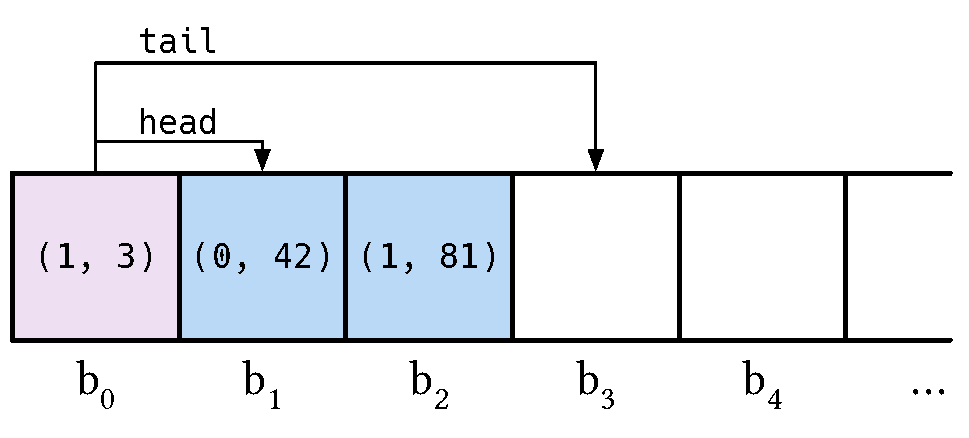
\includegraphics[width=0.8\textwidth]{figs/overview-good.pdf}
    \caption{On-disk layout of a simple log-structured key-value store. Each block holds a (key, value) pair.
    The first block is a superblock that holds pointers to the head and tail of the log.}
    \label{fig:overview:layout}
  \end{subfigure}%
  \quad%
  \begin{subfigure}[t]{0.48\textwidth}
    \centering
    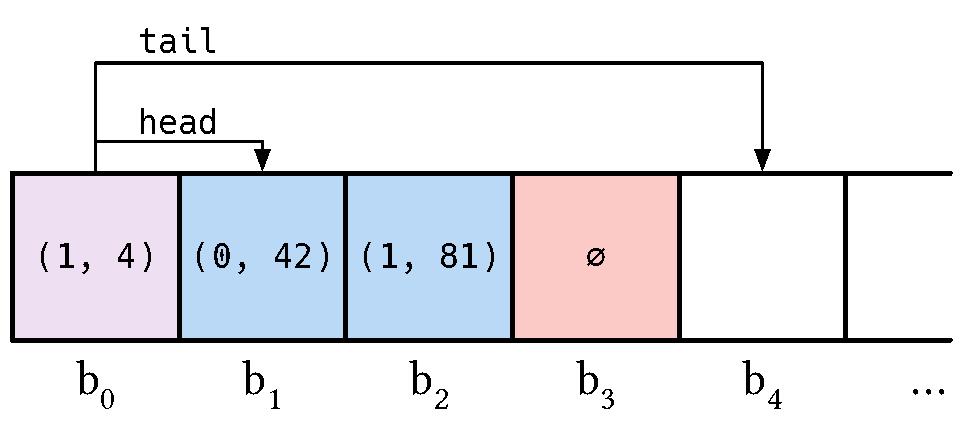
\includegraphics[width=0.8\textwidth]{figs/overview-crash.pdf}
    \caption{Possible on-disk state after a crash, leaving the superblock pointing to a range that includes an invalid block.}
    \label{fig:overview:crash}
  \end{subfigure}
  \caption{The on-disk layout of a simple key-value store. Arrows denote pointers and boxes are blocks.}
  \label{fig:overview}
\end{figure}

While this implementation is functionally correct,
it would not be crash consistent if implemented on a classical storage stack.
The issue is with the ordering of log and superblock writes:
even though the code suggests that the superblock write comes after the log write,
optimizations in the storage stack could reorder the two writes
and lead to a crash state where the superblock is updated but its corresponding new log block is not,
as \cref{fig:overview:crash} shows.
This would leave the \texttt{superblock_tail} pointer referring to an uninitialized disk block.
What we need for consistency is a way to preclude this reordering.
One solution in the \depsynth programming model
would be for the developer to manually implement a \emph{dependency rule}
that prevents this reordering:
%
\begin{lstlisting}[language=py]
  def __init__(self):
    self.rule("superblock", "log", eq)
\end{lstlisting}
%
A dependency rule \lstinline[language=py]{rule("a", "b", eq)}
specifies an ordering constraint:
a write labeled with name \lstinline[language=py]{"a"}
must not be sent to disk until after a write labeled with name \lstinline[language=py]{"b"}.
We say that such a rule means write \lstinline[language=py]{"a"} \emph{depends on} write \lstinline[language=py]{"b"},
or equivalently that write \lstinline[language=py]{"b"} must \emph{happen before} write \lstinline[language=py]{"a"}.
The third argument to \lstinline[language=py]{rule}
is an \emph{epoch predicate} that scopes the rule using the epoch in each label.
Here, the \lstinline[language=py]{eq} predicate
restricts the rule to only apply to pairs of writes whose labels have equal epochs.
% Throughout this paper, we use the notation $\deprule{a}{b}{p}$
% to denote a rule where a write labeled with name $a$ depends on a write labeled with name $b$ under epoch predicate $p$.
This rule means that superblock updates cannot be persisted on disk
until a log block write with the same epoch is persisted first,
ruling out the reordering behavior that could make the log inconsistent.\tighten

% While the developer could specify this dependency rule manually,
% our programming model does not require them to.
% Instead, \depsynth can automatically synthesize this rule, as described next.

\paragraph{Dependency rule synthesis.}
While the developer could specify the above dependency rule manually,
our programming model does not require them to,
and distilling the correct set of rules for a complex storage system is difficult to do by hand.
The challenge is a semantic gap:
the developer's desired high-level consistency property is about the on-disk data structure as a whole,
but the implementation of consistency can only refer to individual block-sized writes.
We bridge this gap with \depsynth, a program synthesis tool
that can \emph{automatically infer} the dependency rules sufficent to make a storage system crash consistent.

\depsynth takes three inputs.
First, it takes as input the implementation of the storage system.
Second, it takes as input a crash consistency predicate,
written as an executable checker over a disk state.
The crash consistency predicate
defines the property that should be true of \emph{every} state of the disk, 
including after crashes.
For our log-structured key-value store,
our desired consistency property is that the \texttt{superblock_tail} pointer
never gets ahead of the blocks that have been written to the log.
We can implement this property by checking that all blocks in the log are valid log blocks 
(we omit an implementation of \texttt{valid} for brevity,
but it could validate a checksum of the block):
%
\begin{lstlisting}[language=py]
  def consistent(self) -> bool:
    ret = True
    for address in range(self.superblock_head, self.superblock_tail):
      block = disk.read(address)
      ret = ret and valid(block)
    return ret
\end{lstlisting}
%
Finally, \depsynth takes as input a collection of \emph{litmus tests},
small programs that exercise the storage system.
Litmus tests are widely used to communicate the semantics of memory consistency models~\cite{alglave:litmus-tool,wickerson:memalloy},
and have also been used to communicate crash consistency models~\cite{bornholt:ferrite}.
A \depsynth litmus test comprises two executable programs \emph{initial} and \emph{main}.
Both programs take as input a reference to the storage system.
The \emph{initial} program sets up some initial state in the system, and cannot crash.
The \emph{main} program manipulates the system state, and can crash at any point.
For example, this is a simple litmus test that starts from a single log entry
and appends two more:
%
\begin{lstlisting}[language=py]
class SingleEntry_TwoAppend(LitmusTest):
  def initial(self, store: KeyValueStore):
    store.put(0, 42)
  
  def main(self, store: KeyValueStore):
    store.put(1, 81)
    store.put(2, 37)
\end{lstlisting}
%
As with previous work on memory consistency models~\cite{alglave:litmus-tool,bornholt:memsynth},
the developer can draw litmus tests from a number of sources:
they may be hand-written by the developer,
drawn from a common set of tests for important properties,
generated automatically by a fuzzer or program enumerator,
or intelligently generated by analyzing the on-disk data structures used by the storage system~\cite{alglave:diy}.

Given these three inputs,
\depsynth automatically synthesizes a set of dependency rules
that suffice to guarantee the crash-consistency predicate holds
on all crash states generated by all litmus tests.
For our example log-structured key-value store,
\depsynth synthesizes two dependency rules:
%
\begin{lstlisting}[language=py]
  def __init__(self):
    self.rule("superblock", "log", eq)
    self.rule("superblock", "superblock", gt)
\end{lstlisting}
%
The first rule is the same rule we hand-wrote earlier.
The second rule fixes a subtle crash-consistency bug in our hand-written implementation:
while the first rule ensures consistency for a \emph{single} put operation,
it still allows \texttt{superblock_tail} to get ahead of the log
if writes from \emph{multiple} puts are reordered with each other
(for example, reordering writes from the first and second puts in the litmus test above).
The second rule prevents this reordering using the \texttt{gt} epoch predicate,
which specifies that a superblock write with epoch $i$
cannot be persisted to disk until all superblock writes with lower epochs $j < i$ are persisted first.
The combination of these rules
precludes the problematic reordering
and guarantees that the superblock always refers to a valid \emph{range} of log blocks,
rather than only requiring the block at \texttt{superblock_tail} to be valid.
% Consistency failures in log writes similar to this one have caused data loss in the ext4 file system~\cite{gribincea:ubuntu-ext4}.

\if 0
\paragraph{Durability properties.}
We can also extend the \depsynth workflow to synthesize implementations
that satisfy stronger durability properties about a storage system.
For example, one durability property our log-structured key-value store should guarantee
is that once a key--value entry is persisted to disk,
it should never be lost by a subsequent crash.
To support such properties, crash consistency predicates in \depsynth
also accept an optional litmus test argument,
allowing them to refer to the expected state of the storage system:
%
\begin{lstlisting}[language=py]
  def consistent2(self, test: LitmusTest) -> bool:
    ret  = self.consistent()
    keys = test.expected_keys()
    for key in keys:
      ret = ret and self.get(key) != None
    return ret
\end{lstlisting}
%
The \texttt{expected_keys} method analyzes the litmus test statically to determine which keys
\emph{must} be present in any crash state of the key-value store.
For example, in the litmus test above,
we know that key \texttt{0} must be present as it is written by the initial method, which cannot crash.

\begin{figure}
  \centering
  \begin{subfigure}[t]{0.48\textwidth}
    \centering
    \includegraphics[width=0.8\textwidth]{example-image-golden}
    \caption{A crash state arising from reordering multiple puts.}
    \label{fig:overview2:put}
  \end{subfigure}%
  \quad%
  \begin{subfigure}[t]{0.48\textwidth}
    \centering
    \includegraphics[width=0.8\textwidth]{example-image-golden}
    \caption{A crash state arising from reordering during garbage collection.}
    \label{fig:overview2:gc}
  \end{subfigure}
  \caption{Two examples of crash-consistency violations that \depsynth can automatically rule out by inferring new dependency rules.}
  \label{fig:overview2}
\end{figure}

To see how this property might be violated,
consider adding garbage collection to the key-value store---%
if the same key is put into the store multiple times,
the previous entries are wasted space that can be reused
(although our toy implementation does not reuse blocks).
One naive garbage collection algorithm just iterates over all blocks in the log,
copies the entries that are still live,
and then moves the head of the journal:
%
\begin{lstlisting}[language=py]
  def garbage_collect(self):
    initial_tail = self.superblock.tail
    for address in range(self.superblock.head, initial_tail):
      block = disk.read(block)
      key, value = from_block(block)
      if value == self.get(key):
        self.put(key, value)
    self.superblock.head = initial_tail
    disk.write(0, to_block(self.superblock), ("superblock", self.counter))
    self.counter += 1
\end{lstlisting}
%
This garbage collection algorithm satisfies the original \texttt{consistent} predicate above,
because the range between the head and tail pointers always contains valid blocks.
But it can violate the durability property in \texttt{consistent2}:

% giving up here, not sure we need the extra detail.

\paragraph{Iterating on storage system design.}
\todo{not sure i need this part. but basically: let's add garbage collection to the log. it's hard and introduces new consistency issues,
but the synthesizer takes care of those automatically. use this to demonstrate ``initial state'' of a litmus test,
to speciofy durability properties.}

\fi

\if 0

\depsynth is a tool for adding crash consistency code to storage systems.
To use \depsynth, developers provide a base system implementation, a crash
consistency property, and a set of example programs that can run over their system.
In this section, we show the design process of a crash consistent system using
\depsynth and how developers use the output of \depsynth.
\todo{make a figure for the input/output behavior of \depsynth?}

\paragraph{A simple key-value store}
\todo{Better transition here? Outline this subsection?}
We start with the design of a simple key-value store that inserts data with \putreq requests,
retrieves data with \get requests, and flushes data to disk with \flush requests.
These requests are synchronous, and in general, \depsynth does not support concurrency.
Our disk model allows the operations \texttt{(read! region location length)},
\texttt{(write! region data location)}, and \texttt{(flush! region)}, which read (possibly cached)
data from disk, write data to disk, and flush data to disk respectively. The disk also allows \texttt{(append! region data)},
which is the same as a \texttt{write!} to the end of the disk region. \texttt{flush!} is important because
writes to disk are not immediately committed, meaning that the write data may still be in a buffer and not
yet actually on the disk. After \texttt{(flush! region)}, all writes to disk region \texttt{region} are committed.
Additionally, data from \texttt{write!} or \texttt{append!} is formatted into one or more pages, and flushing
each page to disk is done atomically. There are no assumptions made about the state of the disk before
a program (i.e. sequence of \putreq, \get, \flush) is run.

One way to design a key-value store is to store metadata and data separately \todo{cite, wisckey, shardstore}.
This allows the implementation of \get to avoid scanning through all of the stored data.
On disk, one region is reserved for an index of metadata, and another region is reserved for
a store of data. On request $\putreq\ K\ V$, our implementation appends the metadata $(K, L, |V|)$
to the index and the data $V$ to the store, where $L$ is the location of $V$
in the store disk region. An implementation of this design is shown in \autoref{fig:kv-single-index}.

\todo{Should probably change code to be imperative/pythonic}

\begin{figure}[h]
  \centering
  \resizebox{\linewidth}{!}{%
    \begin{minipage}{1.03\linewidth}
      \lstinputlisting[language=rosette,xleftmargin=-.5em,firstline=1,basicstyle=\scriptsize\ttfamily]{code/kv-single-index.rkt}
    \end{minipage}}
  \vspace{-.5em}
  \caption{Implementation of a key-value store with a separate metadata index}
  \label{fig:kv-single-index}
\end{figure}

\paragraph{What can go wrong?}
Recall that writes from \texttt{append!} can be buffered by the disk and committed later.
Suppose a user of our key-value store issues a request $\putreq\ '\texttt{a}' \ 7$.
Our implementation would write $('\texttt{a}', 0, 1)$ to the index and $(7)$ to the data store, both of which are
buffered. Since the disk can choose the order of these writes to commit, it chooses to commit
$('\texttt{a}', 0, 1)$ to the index first. Then, before the disk is able to commit $(7)$ to the data store, the
power goes out and the disk crashes. Upon booting back up, the index data is on disk but the actual data $(7)$ is not.
This means that any future requests $\get\ '\texttt{a}'$ could return incorrect data. This is especially bad
because from a users perspective, there is no notification of an error in our system.
\todo{Make figure that shows (old and new) behavior of $\get\ '\texttt{a}'$}

\paragraph{How can we fix this problem?}
There are several ways that storage systems can ensure the crash consistency of their data.
Journaling, copy-on-write, and soft updates are among the most popular ways that systems
implement crash consistency \todo{cite}. In this paper, we focus on implementing crash consistency
with soft updates. Soft updates work by specifying a partial order over disk writes that restricts
when writes can be committed to disk. FeatherStitch \todo{cite} showed that these restrictions can be
specified as dependencies or "write-before" relationships between disk writes, where the relationship
``$A$ depends on $B$'' means that $A$ should only be sent to disk after $B$ is committed on disk.
If we treat these relations as directed edges between disk writes, we get a \textit{dependency graph}.
To fix our example with soft updates, we could make the index write \textit{depend on} the data write.
Then, after any crash, $\get\ '\texttt{a}'$ would either return \texttt{false} (when not all data is committed
before the crash) or the correct value: $7$.

\depsynth generates crash consistency code using the soft updates model.
This gives storage systems built with \depsynth the advantage of faster performance because unlike
other methods of implementing crash consistency, soft updates avoids duplicating writes.
Specifically, \depsynth outputs a set of \textit{rules} that specify how to construct dependencies
between disk writes emitted by the storage system.

\paragraph{Crash Consistency Properties and Dependency Rules}
Now we can discuss precisely what crash consistency means for our basic key-value store. When a disk
crash occurs and later reboots, future calls to $\get\ K$ should either report a failure or should
return some value $V$ where some $\putreq\ K\ V$ was issued before the crash. $\get\ K$ should only
report a failure when the data and metadata for $K$ had not been completely committed before the crash
Concretely, we can encode this crash consistency property by maintaining a reference model that
describes all possible crash consistent behaviors for any sequence of operations on our key-value store.

\todo{make a figure for the reference model and crash consistency property?}

The only way that this property can be broken in our simple key-value store is in the case we previously
discussed: a crash happens after an index write is committed and before the corresponding data write is committed.
As we mentioned, we can avoid this situation by making the index write \textit{depend on} the data write.
In fact, each pair of writes from a \putreq request should have this relationship. \depsynth encodes this fact
as a \textit{dependency rule}, which is a tuple of \textit{parent label}, \textit{child label},
and \textit{timing relation}.
For example, consider the rule that \depsynth outputs for our simple key-value store:

%$$ \texttt{put:append!(index)} \rightarrow_= \texttt{put:append!(data-store)} $$
$$ \deprule{\texttt{put:append!(index)}}{\texttt{put:append!(data-store)}}{=}$$

Here, the parent label is \texttt{put:append(index)}, the child label is \texttt{put:append(data-store)},
and the timing relation is $=$. Parent and child labels match individual disk writes issued by the
system implementation. In this case, the parent would be any write to the index from an \texttt{append!} in the
\texttt{put} function implementation, while the child would be any write to the data store from an \texttt{append!}
in the \texttt{put} implementation. The timing relation specifies if the rule should apply within a single request
or across requests. Here, the timing relation $=$ specifies that the rule should only apply to writes that were
generated by the same \putreq request.

\paragraph{Automatically generating crash consistency rules}
Writing dependency rules requires reasoning about disk states in the presence of a crash, which can
be difficult to do as the complexity of a system increases. \depsynth is a tool for automatically
synthesizing dependency rules, removing this burden from the developer. As input, \depsynth takes
the implementation of the storage system along with the crash consistency property and a set of
example sequences of operations over the system. We call these sequences of operations
\textit{litmus tests}, inspired by work in memory consistency models \todo{cite, ferrite, memory models}.
A set of three litmus tests for our basic key-value store is shown in \autoref{fig:test-set}.
An important point about litmus tests is that when checking for correctness with respect to the crash consistency
property, we only consider crashes that occur during flush points (i.e. whenever \texttt{flush} is called on
a disk region and at the end of the test). This is sufficient because crashing at any
other point has the same affect on the disk state as crashing at the end of the most recent flush.
\todo{I'm not totally sure how to explain this briefly. I think the term "flush point" comes out of nowhere and seems random.}
With these three inputs, \depsynth outputs the dependency rule shown previously.

\begin{figure}[h]
  \centering
  \resizebox{\linewidth}{!}{%
    \begin{minipage}{1.03\linewidth}
      \lstinputlisting[language=rosette,xleftmargin=-.5em,firstline=1,basicstyle=\scriptsize\ttfamily]{code/test-set.rkt}
    \end{minipage}}
  \vspace{-.5em}
  \caption{Set of example requests for our key-value store}
  \label{fig:test-set}
\end{figure}

As the complexity of our system and of crash behaviors increases, determining
correct ordering rules becomes more difficult for developers.
To demonstrate this point, we improve upon the previous key-value store design by improving
space efficiency in the index. The amount of space used by the index was dependent on the number of \putreq
requests in the old design. This new design will improve upon this, making the size of the index instead
dependent on the number of keys stored. We can do this by adding a \clean operation which removes
all overwritten metadata from the index.

\begin{figure}[h]
  \centering
  \resizebox{\linewidth}{!}{%
    \begin{minipage}{1.03\linewidth}
      \lstinputlisting[language=rosette,xleftmargin=-.5em,firstline=1,basicstyle=\scriptsize\ttfamily]{code/kv-wrong-index.rkt}
    \end{minipage}}
  \vspace{-.5em}
  \caption{Naive implementation of a key-value store with \clean}
  \label{fig:kv-wrong-index}
\end{figure}

A naive new implementation for \clean would read the index, remove overwritten metadata for all keys that
appear more than once, and write the result back out to the index as seen in \autoref{fig:kv-wrong-index}.
After updating the implementation and litmus test set and running \depsynth again, we get the following result:
\texttt{No rules found}.

This means that \depsynth was unable to find a set of rules that guarantees our crash consistency
property under all crash behaviors. \depsynth also outputs the litmus test that caused it to fail,
shown in \autoref{fig:failing-test}. To help understand what went wrong, the state of the data store
and index after each request is shown in a comment. The data within \texttt{*...*} has been flushed to disk.
\todo{This is not something that's output by \depsynth, I just put it here to help explain what's going on. I could make \depsynth output it though, but that seems like a minute implementation detail}

\begin{figure}[h]
  \centering
  \resizebox{\linewidth}{!}{%
    \begin{minipage}{1.03\linewidth}
      \lstinputlisting[language=rosette,xleftmargin=-.5em,firstline=1,basicstyle=\scriptsize\ttfamily]{code/failing-test.rkt}
    \end{minipage}}
  \vspace{-.5em}
  \caption{Test that causes \depsynth to return \texttt{No rules found}}
  \label{fig:failing-test}
\end{figure}

Recall that while single writes $(K, L, |V|)$ to the index are atomic (since it fits in a page),
writing the entire contents of the index is not. Consider a crash that occurs after the test case in
\autoref{fig:failing-test}, before all data is committed to disk. Since the crash happens while the
index is being updated from \clean, previous entries could be incompletely overwritten. Metadata that
was completely flushed to disk by \flush could be lost, breaking our crash consistency property.
This is exactly the behavior in \autoref{fig:failing-test} that causes \depsynth to fail.

Understanding this, we can adjust the design of our key-value store to avoid overwriting old entries
and make crash consistency possible. Instead of writing the updated index to the same disk region,
our key-value store will keep two distinct regions, alternating between them when updating the
index. Additionally, our key-value store needs to reserve a distinct block to update the pointer
indicating the current set of index region being used. On a \clean operation, we read the old index
and remove outdated metadata, but instead of writing to the same index region, we update the index
pointer and write the updated index metadata to the previously unused index region. Our new
implementation is shown in \autoref{fig:kv-double-index}.

\begin{figure}[h]
  \centering
  \resizebox{\linewidth}{!}{%
    \begin{minipage}{1.03\linewidth}
      \lstinputlisting[language=rosette,xleftmargin=-.5em,firstline=1,basicstyle=\scriptsize\ttfamily]{code/kv-double-index.rkt}
    \end{minipage}}
  \vspace{-.5em}
  \caption{Implementation of a key-value store design with \clean}
  \label{fig:kv-double-index}
\end{figure}

With this updated key-value store implementation, we can run \depsynth again to find a new set of
rules that ensure our crash consistency property holds. \depsynth outputs the following new rules.

\begin{align*}
  \texttt{put:append!(index)} &\rightsquigarrow_= \texttt{put:append!(data-store)} \\
  \texttt{clean:update!(index-pointer)} &\rightsquigarrow_= \texttt{clean:append!(data-store)} \\
  \texttt{clean:update!(index-pointer)} &\rightsquigarrow_> \texttt{put:append!(data-store)}
\end{align*}

The first rule is the same as the rule from our simpler example.
The second rule states that the update to the index pointer should wait until the updated
index metadata has been written. Without this rule, a crash could allow the index pointer
to be updated to an old (and possibly empty) version of the index.
The third rule states a stronger requirement: that the update to the index pointer should
wait until \emph{all} writes to the data store from previous \putreq requests have completed.\tighten

\fi


\section{Reasoning About Crash Consistency}\label{sec:problem}

The \depsynth workflow includes a new high-level interface for building storage systems
and a synthesis tool for automatically making those systems crash consistent.
This section describes the high-level interface,
including labeled writes and dependency rules,
and presents a logical encoding for reasoning about crashes of systems that use this interface.
\Cref{sec:alg} then presents the \depsynth synthesis algorithm for inferring
sufficient dependency rules to make a storage system crash consistent.\tighten

\subsection{Disk Model and Dependency Rules}\label{sec:problem:disk}

In the \depsynth programming model,
storage systems run on top of a disk model $d$ that provides two operations:
\begin{itemize}
\item $d.{\tt write}(a, v, l)$: write a data block $v$ to disk address $a$ with label $l$
\item $d.{\tt read}(a)$: read a data block at disk address $a$
\end{itemize}
We assume that single-block write operations are atomic, as in previous work~\cite{sigurbjarnarson:yggdrasil,chen:fscq}.
These interfaces are similar to the standard POSIX \texttt{pwrite} and \texttt{pread} APIs,
except that the \texttt{write} operation additionally takes as input a \emph{label} for the write.
A label $l = \langle n, t \rangle$ is a pair of a \emph{name} string $n$ and an \emph{epoch} integer $t$.
Labels allow the developer to provide identities for each write their system performs,
which dependency rules (described below) can inspect to enforce ordering requirements.
Although the two components of a label together identify a write,
developers use them for separate purposes:
the name indicates which on-disk data structure the write targets,
while the epoch associates related writes with different names.
Names are strings but are not interpreted by our workflow
other than to check equality between them.
Epochs are integers that dependency rules use as logical clocks to impose orderings on related writes.

% This definition closely follows the ``asynchronous disk'' model of Yggdrasil~\cite{sigurbjarnarson:yggdrasil},
% except that the write operation additionally takes as input a label $l$.
% These labels are how the cache applies its dependency rules to guarantee ordering,
% as described below.

% The ordering-aware buffer cache is inspired by previous higher-level storage APIs
% such as those used by Featherstitch~\cite{frost:featherstitch} and ShardStore~\cite{bornholt:s3},
% which also provide interfaces for specifying ordering requirements for writes.
% But these interfaces are imperative,
% requiring the developer to manually construct a dependency graph

% Storage systems use \emph{disks} to persist their state.
% The precise guarantees of these disks vary by media type (SSD, HDD, tape, etc.),
% configuration (volatile or non-volatile caches, append-only media, etc.),
% and sometimes even by manufacturer.
% Rather than modeling all these variations directly,
% we assume that storage applications run on top of an \emph{ordering-aware buffer cache},
% similar to those provided by Featherstitch~\cite{frost:featherstitch} or ShardStore~\cite{bornholt:s3}.
% An ordering-aware buffer cache is a layer low in the storage stack,
% and is parameterized by a set of \emph{dependency rules} that define ordering requirements for writes to disk
% (and which \depsynth will synthesize).
% The ordering-aware buffer cache takes as input individual disk operations
% and guarantees to send them to the disk in a way that respects the dependency rules;
% if the system crashes at any point,
% the resulting state on the disk will be consistency with the dependency rules.
% We trust the correctness of the ordering-aware buffer cache,
% and so its implementation details are out of scope for \depsynth,
% but could make use of a variety of consistency primitives provided by disks
% including force-unit-access writes, cache flush commands, or ordering barriers.

% An ordering-aware buffer cache $d$ provides three operations:
% \begin{itemize}
% \item $d_R.{\tt write}(a, v, l)$: write a data block $v$ to disk address $a$ with label $l$;
% \item $d_R.{\tt read}(a)$: read a data block at disk address $a$;
% \item $d_R.{\tt flush}()$: block until all previous writes are flushed to disk.
% \end{itemize}
% We assume that single-block write operations are atomic, as in previous work~\cite{sigurbjarnarson:yggdrasil,chen:fscq}.
% This definition closely follows the ``asynchronous disk'' model of Yggdrasil~\cite{sigurbjarnarson:yggdrasil},
% except that the write operation additionally takes as input a label $l$.
% These labels are how the cache applies its dependency rules to guarantee ordering,
% as described below.
% % Note that we do not model read operations as they do not participate in ordering requirements.

\paragraph{Dependency rules.}
% Most existing crash consistency protocols are imperative:
% the protocol is intertwined with the implementation of the storage system itself,
% either directly by inserting consistency primitives into the code (e.g., \texttt{fsync})
% or indirectly by constructing ordering constraints at run time (e.g., \emph{patchgroups} in Featherstitch~\cite{frost:featherstitch}).
% These approaches make it difficult to automatically synthesize a new crash consistency protocol,
% as the synthesis needs to be aware of, and integrated with, the often complex implementation of the storage system.

% The ordering-aware buffer cache interface can be configured with declarative \emph{dependency rules} for defining consistency requirements.
\depsynth synthesizes declarative \emph{dependency rules}
to enforce consistency requirements for a storage system that uses labeled writes.
%
\begin{definition}[Dependency rule]\label{def:dependency-rule}
A \emph{dependency rule} $\deprule{n_1}{n_2}{p}$
comprises two names $n_1$ and $n_2$ and an epoch predicate $p(t_1, t_2)$ over pairs of epochs.
Given two labels
$l_a = \langle n_a, t_a \rangle$
and
$l_b = \langle n_b, t_b \rangle$,
we say that a dependency rule $\deprule{n_1}{n_2}{p}$
\emph{matches} $l_a$ and $l_b$
if $n_a = n_1$, $n_b = n_2$, and $p(t_a, t_b)$ is true.
\end{definition}

% \todo{Define dependency safety in this section, 
%  and cross reference it in the last sentence of the next section.}
\noindent
Dependency rules define ordering requirements over all writes with labels that match them,
and the dependency-aware buffer cache enforces these rules at run time.
More precisely, the dependency-aware buffer cache enforces \emph{dependency safety}
for all writes it sends to disk:
%
\begin{definition}[Dependency safety]\label{def:dependency-safety}
A dependency-aware buffer cache maintains
\emph{dependency safety} for a set of dependency rules $R$ if,
whenever a storage system issues two writes
$d.{\tt write}(a_1, s_1, l_1)$ and
$d.{\tt write}(a_2, s_2, l_2)$,
and a rule $\deprule{n_a}{n_b}{p} \in R$ matches $l_1$ and $l_2$,
then the cache ensures the write to $a_1$ does not persist until the write to $a_2$ is persisted on disk.
\end{definition}
%
\noindent
In other words, all crash states of the disk that include the effect of the first write
must also include the effect of the second write.
\Cref{sec:problem:crashes} will specify dependency safety more formally
by defining the crash behavior of a disk in first-order logic. 
% Given a set of rules $R$,
% we write $d_R$ for an ordering-aware buffer cache
% that has been configured with the rules in $R$.

The epoch predicate of a dependency rule
reduces the scope of the rule to only apply to some writes labeled with the relevant names.
Given two labels $l_1 = \langle n_1, t_1 \rangle$ and $l_2 = \langle n_2, t_2 \rangle$,
a dependency rule $\deprule{n_1}{n_2}{p}$ can use one of three epoch predicates: $=$, 
$>$, and $<$, which restrict the rule to apply only when 
$t_1 = t_2$,  $t_1 > t_2$, and $t_1 < t_2$, respectively. 
These variations allow dependency rules to specify ordering requirements over unbounded executions of the storage system
without adding unnecessary dependencies between \emph{all} operations with certain names.

Together, the name and epoch components of labels
allow dependency rules to define a variety of important consistency requirements,
depending on how the developer chooses to label their writes.
For example, if all writes generated by a related operation
(e.g., a top-level API operation like \texttt{put} in a key-value store)
share the same epoch $t$,
then rules using the $=$ epoch predicate can impose consistency requirements on individual operations,
such as providing transactional semantics.
As another example, rules using the $>$ epoch predicate
can be used as barriers for all previous writes,
and so can help to implement operations like garbage collection that manipulate an entire data structure.\tighten

\paragraph{Dependency-aware buffer cache.}
At run time,
storage systems implemented with the \depsynth programming model
execute on top of a \emph{dependency-aware buffer cache}.
This buffer cache is configured with a set of dependency rules at initialization time,
and enforces those rules on all writes executed by the storage system.

The dependency-aware buffer cache is inspired by previous higher-level storage APIs
such as those used by Featherstitch~\cite{frost:featherstitch} and ShardStore~\cite{bornholt:s3},
which also provide interfaces for specifying ordering requirements for writes.
Both of these interfaces are imperative:
they require the developer to manually construct a dependency graph for each write they execute,
and so closely intertwine the ordering requirements with the implementation,
as constructing these graphs requires sharing graph nodes 
(\emph{patchgroups} in Featherstitch
and \emph{dependencies} in ShardStore)
across threads and operations.
In contrast, the dependency-aware buffer cache interface is declarative:
the dependency rules are configured once,
and then automatically applied to all relevant writes
without requiring the developer to manually construct graphs
or invoke consistency primitives like \texttt{fsync}.

The implementation details of the dependency-aware buffer cache
are outside the scope of this chapter and follow the examples of Featherstitch and ShardStore.
An implementation could use a variety of consistency and durability primitives provided by disks,
including force-unit-access writes, cache flush commands, or ordering barriers.
We trust the correctness of the dependency-aware buffer cache,
and specifically we assume it enforces dependency safety (\cref{def:dependency-safety}).


% and so often require manually sharing graphs across threads or operations.
% and share these graphs across writes when they need to express larger 
% But these interfaces are imperative,
% requiring the developer to manually construct a dependency graph

% if the storage system executes two writes $w_1$ and $w_2$ with labels $l_1$ and $l_2$
% a write with name $n_1$ cannot be persisted to disk
% until a write with label $n_2$ is first persisted to disk
% For a rule $\deprule{l_1}{l_2}{}$, we say that the write $l_1$ \emph{depends on} the write $l_2$.
% We assume that the ordering-aware buffer cache $d_R$,
% parameterized by a set of dependency rules $R$,
% guarantees a \emph{dependency safety} property:
% for all rules $\deprule{l_1}{l_2}{} \in R$,
% if the application executes two writes
% $d_R.{\tt write}(a_1, s_1, l_1)$ and
% $d_R.{\tt write}(a_2, s_2, l_2)$,
% then all crash states of the disk that include the effect of the write with label $l_1$
% also include the effect of the write with label $l_2$.
% \Cref{sec:problem:crashes} will specify this property more precisely
% by defining the crash behavior of a disk in first-order logic.
% This safety property applies only if both writes have been executed even if the application never executes a write with label $l_2$,
% in which case the write with label $l_1$ cannot appear in \emph{any} crash state.
% The next section 

% Labels are provided for each write by the storage system.
% These labels may be written manually by the developer,
% but can often be provided automatically
% by using static or dynamic information about the call to $d_R.{\tt write}$,
% such as the module the call site is in or the call stack at run time.
% The resulting labels are uninterpreted by the buffer cache,
% other than being able to check equality between two labels for rule application.

% \paragraph{Label Timestamps.}
% While uninterpreted labels are, in principle, expressive enough to implement interesting crash consistency protocols,
% they make it inconvenient to specify some consistency requirements such as barriers.
% We therefore extend the dependency rule language and labels with a notion of \emph{timestamps}.
% We assume each label has an associated timestamp $t(l)$,
% and write $l @ \tau$ for a label $l$ with timestamp $\tau$ where necessary.
% Dependency rules can then quantify over timestamps:
% a dependency rule $\deprule{l_1}{l_2}{=}$ applies to all writes with labels $l_1$ and $l_2$
% where $t(l_1) = t(l_2)$, and similarly for rules $\deprule{l_1}{l_2}{<}$ and $\deprule{l_1}{l_2}{>}$.
% \todo{not sure i understand where one would ever use < rules --jb}

% Timestamps allow dependency rules to specify barrier behavior in unbounded executions of a system.
% For example, a rule $\deprule{\texttt{superblock}}{\texttt{data}}{>}$
% allows writes to a superblock to act as barriers for previous writes to data blocks:
% a specific superblock write (e.g., with label $\texttt{superblock} @ 10$)
% must persist after all \emph{previous} data writes (e.g., all writes with labels $\texttt{data} @ \tau$ for $\tau < 10$),
% but places no restriction on the ordering of \emph{future} data writes.
% As this notation is purely for convenience---%
% any dependency rule with a timestamp quantifier can be grounded into a (possibly infinite) set of rules without timestamp quantifiers---%
% the rest of our formalization omits timestamps,
% but the \depsynth implementation includes them.
% %This extension i

\subsection{Storage Systems and Litmus Tests}\label{sec:problem:tests}

To apply \depsynth, developers provide three inputs:
a storage system implementation,
a collection of litmus tests that exercise the storage system,
and a crash consistency predicate for the system.

\paragraph{Storage system implementations.}
Developers implement a storage system for \depsynth
by defining a collection of API operations \sys and an implementation function for each operation:
%
\begin{definition}[Storage system implementation]\label{def:storage-system}
A \emph{storage system implementation} $\sys = \{O_a, O_b, \dots\}$
is a set of API operations $O_i$ and,
for each $O_i$,
an \emph{implementation function} $I_{O_i}(d, \vec{x})$
that takes as input a disk state $d$ and a vector of other inputs $\vec{x}$
and issues write operations to mutate disk $d$.
\end{definition}
%
\noindent
\depsynth requires implementation functions to support being symbolically evaluated
with respect to a symbolic disk state $d$.
In this work, we use Rosette~\cite{torlak:rosette} as our symbolic evaluator;
this allows implementation functions to be written in Racket
and automatically lifted to support the necessary symbolic evaluation,
so long as their executions are deterministic and bounded.

We say that a \emph{program} $P$ is a sequence of calls $[O_1(\vec{x}_1), \dots, O_n(\vec{x}_n)]$
to API operations $O_i \in \sys$.
Given a program $P$,
we write $\evaluate{P}{\sys}$ for the function that symbolically evaluates each $I_{O_i}(d, \vec{x}_i)$ in turn,
starting from a symbolic disk $d$,
and returns a \emph{trace} of labeled write operations $[w_1, \dots, w_n]$ that the program performed.
The trace does not need to include read operations
as they cannot participate in ordering requirements.

% \depsynth synthesizes dependency rules that guarantee crash consistency for a specific storage system.
% Developers specify their storage application to \depsynth by providing an interpreter function $\interpret{P}$
% that reduces a straight-line, deterministic program $P$
% to the trace of buffer cache write operations $[w_1, \dots, w_n]$ the program performs.
% %where each operation $o_i$ is either a write operation ${\tt write}(a_i, v_i, l_i)$ or a flush operation ${\tt flush}$.
% The trace does not include read operations as they cannot participate in ordering requirements.
% % We do not make any other assumptions about the language of programs $P$,
% % and \depsynth does not need to be aware of the syntax or semantics of the language.
% \todo{somehow, we need to explain the execution model -- rosette, self-finitizing, etc --jb}
% \todo{probably want to be more explicit somewhere about limitations -- straight-line code}

\paragraph{Litmus tests.}
\depsynth synthesizes dependency rules from a set of example \emph{litmus tests},
which are small programs that exercise the storage system
and demonstrate its desired consistency behavior.
A litmus test $T = \langle P_\emph{initial}, P_\emph{main} \rangle$
is a pair of programs
that each invoke operations of the storage system.
The initial program $P_\emph{initial}$ sets up an initial state of the storage system by,
for example,
prepopulating the disk with files or objects.
It will be executed starting from an empty disk, and cannot crash.
The main program $P_\emph{main}$ then tests the behavior of the storage system
starting from that initial state.
\depsynth will exercise all possible crash states of the main program.

Litmus tests are widely used to communicate the semantics of memory consistency models to developers~\cite{alglave:litmus-tool,wickerson:memalloy},
and have also been used to communicate crash consistency~\cite{bornholt:ferrite}
and to search for crash consistency bugs in storage systems~\cite{mohan:crashmonkey}.
\depsynth is agnostic to the source of the litmus tests it uses
so long as they fit the definition of a program
(i.e., are straight-line and deterministic).
% They may be hand-written by the developer,
% drawn from a common set of tests for important properties,
% or generated automatically by a fuzzer or program enumerator
% (or a combination of all three).

\paragraph{Crash consistency predicates.}
To define crash consistency for their system,
developers also provide a \emph{crash-consistency predicate} $\consistent{d}$
that takes a disk state $d$ and returns whether the disk state should be considered consistent.
The crash-consistency predicate should include representation invariants
for the storage system's on-disk data structures.
For example, a file system like ext2 might require that all block pointers in inodes
refer to blocks that are allocated (i.e., no dangling pointers).
These properties correspond to those that can be checked by an \texttt{fsck}-like checker~\cite{henson:fsck}.
The crash-consistency predicate can also include stronger properties
such as checking the atomic-replace-via-rename property for POSIX file systems~\cite{bornholt:ferrite,pillai:appcrash}.

\subsection{Reasoning About Crashes}\label{sec:problem:crashes}

To reason about the crash behaviors of a storage system,
we encode the semantics of dependency rules and litmus tests in first-order logic
based on existing work on storage verification~\cite{sigurbjarnarson:yggdrasil}.
We first encode the behavior of a single write operation,
and then extend that encoding to executions of entire programs.

\paragraph{Write operations.}
We model the behavior of a disk write operation as a transition function
$f_\texttt{write}(d, a, v, s)$,
that takes four inputs:
the current disk state $d$,
the disk address $a$ to write to,
the new block value $v$ to write,
and a \emph{crash flag} $s$,
a boolean that is used to encode the effect of a crash on the resulting disk state.
Given these inputs, $f_\texttt{write}$ returns the resulting disk state after applying the operation.
The effect of a write operation is visible on the disk only if $s$ is true:\tighten
\begin{align*}
    f_\texttt{write}(d, a, v, s) = d[a \mapsto \texttt{if}\ s\ \texttt{then}\ v \ \texttt{else}\ d(a)].
\end{align*}

\paragraph{Program executions.}
Given the trace of write operations $[w_1, \dots, w_n] = \evaluate{P}{\mathcal{O}}$
executed by a program $P$ against storage system $\mathcal{O}$,
and for each write its corresponding crash flag $s_i$,
we can define the final disk state of the program
by just applying the transition function in sequence:
\begin{align*}
    \run{[\texttt{write}(a_1, v_1, l_1), w_2, \dots, w_n]}{[s_1, \dots, s_n]}{d} &= \run{[w_2, \dots, w_n]}{[s_2, \dots, s_n]}{f_\texttt{write}(d, a_1, v_1, s_1)} \\
    \run{[]}{[]}{d} &= d
\end{align*}
We call the vector $\vec{s} = [s_1, \dots, s_n]$ of crash flags for each operation in the trace
a \emph{crash schedule}.

Not all crash schedules are possible.
At run time, the dependency-aware buffer cache
constrains the set of \emph{valid crash schedules}
by applying the dependency rules it is configured with:

\begin{definition}[Valid crash schedule]\label{def:valid-schedule}
Let $[w_1, \dots, w_n] = \evaluate{P}{\mathcal{O}}$
be the trace of operations executed by a program $P$ on storage system $\mathcal{O}$,
$R$ be a set of dependency rules,
and $\vec{s} = [s_1, \dots, s_n]$
the crash schedule for the trace.
The crash schedule $\vec{s}$ is \emph{valid} for the program $P$
and set of rules $R$,
written $\valid{\vec{s}}{P}{R}$,
if for all operations $w_i = \texttt{write}(a_i, v_i, l_i)$
and $w_j = \texttt{write}(a_j, v_j, l_j)$,
whenever there exists a rule $\deprule{n_a}{n_b}{p} \in R$ that matches $l_i$ and $l_j$,
then $s_i \rightarrow s_j$.
\end{definition}
%
\noindent
This definition is a logical encoding of dependency safety (\cref{def:dependency-safety}):
if $s_i \rightarrow s_j$,
then write $w_j$ is guaranteed to be persisted on disk
whenever write $w_i$ is.

% Finally, both operations take as input a \emph{crash schedule} $\vec{s} = \langle \onbool, \syncbool \rangle$,
% a pair of booleans that are used to encode the effect of a crash on the resulting disk state.
% The $\onbool$ variable indicates whether the operation was executed
% (the machine was ``on'' when executing that operation),
% and the $\syncbool$ variable indicated whether the effect of the operation
% was persisted to disk by the buffer cache.
% The effect of a write operation is visible on the disk only if both $\onbool$ and $\syncbool$ are true:
% \begin{align*}
%     f_\texttt{write}(d, a, v, \langle \onbool, \syncbool \rangle) = d[a \mapsto \texttt{if}\ \onbool \land \syncbool\ \texttt{then}\ v \ \texttt{else}\ d(a)].
% \end{align*}
% A flush operation does not directly affect the state of the disk;
% it instead acts as a barrier by constraining the crash schedules of other writes,
% as described below:
% \begin{align*}
%     f_\texttt{flush}(d, \langle \onbool, \syncbool \rangle) = d.
% \end{align*}

% \paragraph{Program executions.}
% Given the trace of buffer cache operations $[o_1, o_2, \dots, o_n] = \interpret{P}{d}$
% executed by a program $P$,
% and for each operation a corresponding crash schedule $\vec{s}_i = \langle \onbool_i, \syncbool_i \rangle$,
% we can define the final disk state of the program
% by just applying each relevant transition function in sequence:
% \begin{align*}
%     \run{[\texttt{write}(a_1, v_1, l_1), o_2, \dots, o_n]}{d} &= \run{[o_2, \dots, o_n]}{f_\texttt{write}(d, a_1, v_1, \langle \onbool_1, \syncbool_2 \rangle} \\
%     \run{[\texttt{flush}(), o_2, \dots, o_n]}{d} &= \run{[o_2, \dots, o_n]}{f_\texttt{flush}(d, \langle \onbool_1, \syncbool_2 \rangle} \\
%     \run{[]}{d} &= d
% \end{align*}
% However, in a program that executes more than one buffer-cache operation,
% not all crash schedules correspond to possible crash states.
% For example, crashes must respect program order,
% % (if a program crashed before reaching an operation $o_i$,
% % no operation after $o_i$ can be present in the crash state),
% the semantics of \texttt{flush} operations,
% and the guarantees of the ordering-aware buffer cache.
% We encode these requirements by constraining
% what it means for a crash schedule to be \emph{valid}:

% \begin{definition}[Valid crash schedule]\label{def:valid-schedule}
% Let $[o_1, o_2, \dots, o_n] = \interpret{P}{d_R}$
% be the trace of operations executed by a program $P$
% on the ordering-aware buffer cache $d_R$,
% and let $\vec{s} = [\vec{s}_1, \dots, \vec{s}_n]$
% be the crash schedule for each operation $o_i$.
% The crash schedule $\vec{s}$ is \emph{valid} for the program $P$
% and set of rules $R$,
% written $\valid{\vec{s}}{P}{R}$,
% if it satisfies four constraints
% for all operations $o_i$ and $o_j$:
% \begin{enumerate}
%     \item $\syncbool_i \rightarrow \onbool_i$ (persistence order)
%     \item If $j < i$, then $\onbool_i \rightarrow \onbool_j$ (program order)
%     \item If $o_i = \texttt{flush}()$, $o_j = \texttt{write}(a_j, v_j, l_j)$, and $j < i$, then $\onbool_i \rightarrow \syncbool_j$ (flush semantics)
%     \item If $o_i = \texttt{write}(a_i, v_i, l_i)$, $o_j = \texttt{write}(a_j, v_j, l_j)$, and $\deprule{l_i}{l_j}{} \in R$, then $\syncbool_i \rightarrow \syncbool_j$ (dependency safety). 
% \end{enumerate}
% \end{definition}

% The final constraint encodes the correctness guarantee for an ordering-aware buffer cache
% from \cref{sec:problem:disk}:
% the buffer cache $d_R$ guarantees to commit writes to disk
% in an order that respects all dependency rules in $R$.
% \todo{give an example of a valid crash schedule? --jb}

% \subsection{Dependency Rule Synthesis}

Finally, we can define crash consistency for a litmus test $T = \langle P_\emph{initial}, P_\emph{main} \rangle$
as a function of a set of dependency rules $R$:

\begin{definition}[Single-test crash consistency]\label{def:crash-consistent}
Let $T = \langle P_\emph{initial}, P_\emph{main} \rangle$ be a litmus test.
Let $d_\emph{initial} = \run{\evaluate{P_\emph{initial}}{\mathcal{O}}}{\vec{\top}}{d_0}$
be the disk state reached by running the program $P_\emph{initial}$
against storage system $\mathcal{O}$
on the all-true (i.e., crash-free) crash schedule $\vec{\top}$ starting from the empty disk $d_0$.
A set of dependency rules $R$
makes $T$ crash consistent
if, for all crash schedules $\vec{s}$ such that $\valid{\vec{s}}{P_\emph{main}}{R}$ is true,
$\consistent{\run{\evaluate{P_\emph{main}}{\mathcal{O}}}{\vec{s}}{d_\emph{initial}}}$ holds.
\end{definition}

\begin{example}\label{sec:problem:example}
  \normalfont
Consider the \texttt{SingleEntry_TwoAppend} litmus test from \cref{depsynth:s:overview}.
Interpreting the initial and main programs gives two traces:
%
\begin{align*}
    \interpret{P_\emph{initial}} &= [\texttt{write}(1, \texttt{to_block}((0, 42)), \langle \textsf{log}, 0 \rangle), \\
                                 &\quad\ \  \texttt{write}(0, \texttt{to_block}((1, 2)),  \langle \textsf{superblock}, 0 \rangle)] \\
    \interpret{P_\emph{main}}    &= [\texttt{write}(2, \texttt{to_block}((1, 81)), \langle \textsf{log}, 1 \rangle), \\
                                 &\quad\ \  \texttt{write}(0, \texttt{to_block}((1, 3)),  \langle \textsf{superblock}, 1 \rangle), \\
                                 &\quad\ \  \texttt{write}(3, \texttt{to_block}((2, 37)), \langle \textsf{log}, 2 \rangle), \\
                                 &\quad\ \  \texttt{write}(0, \texttt{to_block}((1, 4)),  \langle \textsf{superblock}, 2 \rangle)]
\end{align*}
%
Let $\vec{s} = [s_1, s_2, s_3, s_4]$ be a crash schedule for $P_\emph{main}$.
Applying the two synthesized rules from \cref{depsynth:s:overview}
restricts the valid crash schedules (\cref{def:valid-schedule}):
%
\begin{itemize}
\item $\deprule{\textsf{superblock}}{\textsf{log}}{=}$ requires $s_2 \rightarrow s_1$ and $s_4 \rightarrow s_3$.
\item $\deprule{\textsf{superblock}}{\textsf{superblock}}{>}$ requires $s_4 \rightarrow s_2$.
\end{itemize}
%
Combined, these constraints yield seven valid crash schedules.
Besides the two trivial crash schedules $\vec{s} = \vec{\top}$ and $\vec{s} = \vec{\bot}$,
the other five crash schedules yield five distinct disk states:
% 0: (list (cons b2 #f) (cons b1 #f) (cons b4 #f) (cons b3 #f)) <-- all #f
% 1: (list (cons b2 #f) (cons b1 #t) (cons b4 #f) (cons b3 #f)) <-- only first log block
% 2: (list (cons b2 #t) (cons b1 #t) (cons b4 #f) (cons b3 #f)) <-- first log block + first superblock
% 3: (list (cons b2 #t) (cons b1 #t) (cons b4 #f) (cons b3 #t)) <-- first log block + first superblock + second log block
% 4: (list (cons b2 #f) (cons b1 #t) (cons b4 #f) (cons b3 #t)) <-- both log blocks
% 5: (list (cons b2 #t) (cons b1 #t) (cons b4 #t) (cons b3 #t)) <-- all #t
% 6: (list (cons b2 #f) (cons b1 #f) (cons b4 #f) (cons b3 #t)) <-- only second log block
\begin{enumerate}[label={\raisebox{2\baselineskip}[0pt][0pt]{(\arabic*)}},ref=(\arabic*)]
\item 
\begin{minipage}[b]{0.5\textwidth}
$[s_1 = \top, s_2 = \bot, s_3 = \bot, s_4 = \bot]$\\
(only the first log block is on disk) \\
\end{minipage}\quad%
\begin{minipage}{0.4\textwidth}
\vspace{-1.2em}
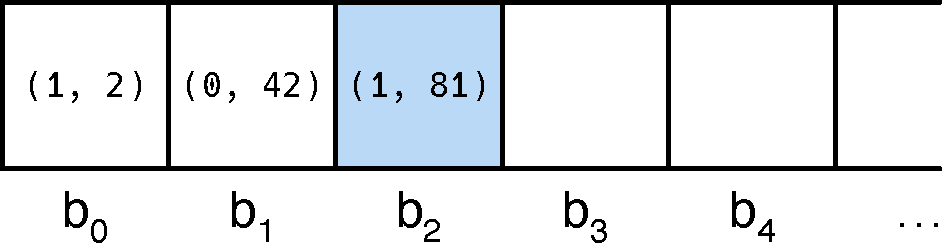
\includegraphics[width=\textwidth]{figs/sec3-1.pdf}
\end{minipage}
\label{sec:problem:loststate}
\item 
\begin{minipage}[b]{0.5\textwidth}
$[s_1 = \bot, s_2 = \bot, s_3 = \top, s_4 = \bot]$\\
(only the second log block is on disk) \\
\end{minipage}\quad%
\begin{minipage}{0.4\textwidth}
\vspace{-1.2em}
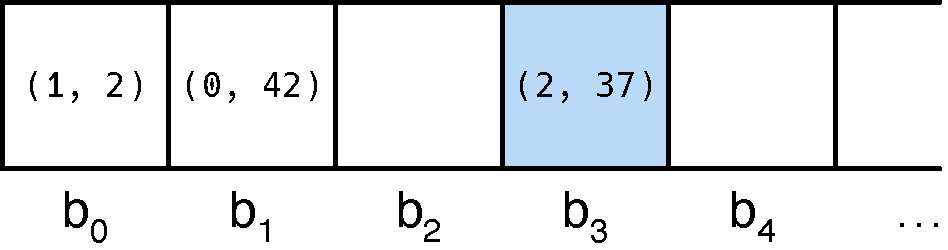
\includegraphics[width=\textwidth]{figs/sec3-2.pdf}
\end{minipage}

\item 
\begin{minipage}[b]{0.5\textwidth}
$[s_1 = \top, s_2 = \bot, s_3 = \top, s_4 = \bot]$\\
(both log blocks are on disk) \\
\end{minipage}\quad%
\begin{minipage}{0.4\textwidth}
\vspace{-1.2em}
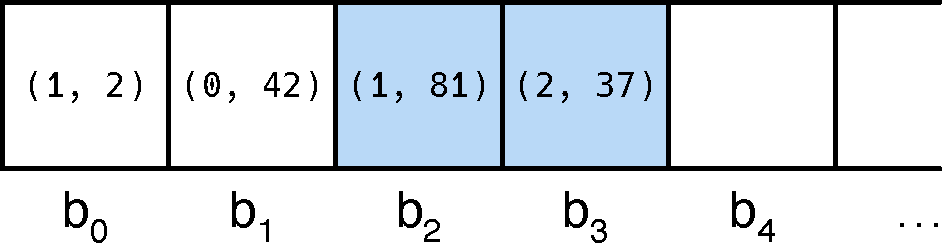
\includegraphics[width=\textwidth]{figs/sec3-3.pdf}
\end{minipage}

\item 
\begin{minipage}[b]{0.5\textwidth}
$[s_1 = \top, s_2 = \top, s_3 = \bot, s_4 = \bot]$\\
(the first log block and first superblock write are on disk)
\end{minipage}\quad%
\begin{minipage}{0.4\textwidth}
\vspace{-1.2em}
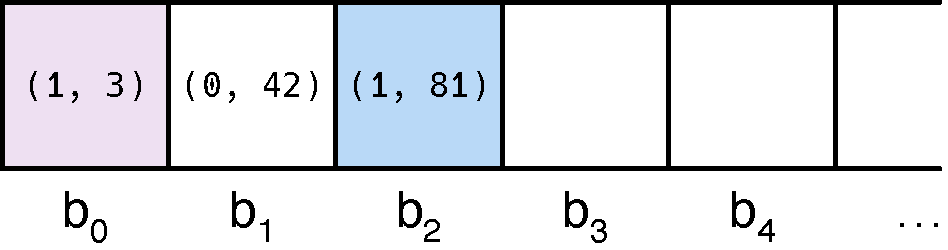
\includegraphics[width=\textwidth]{figs/sec3-4.pdf}
\end{minipage}

\item 
\begin{minipage}[b]{0.5\textwidth}
$[s_1 = \top, s_2 = \top, s_3 = \top, s_4 = \bot]$\\
(the first log block, first superblock write, and second log block are on disk)
\end{minipage}\quad%
\begin{minipage}{0.4\textwidth}
\vspace{-1.2em}
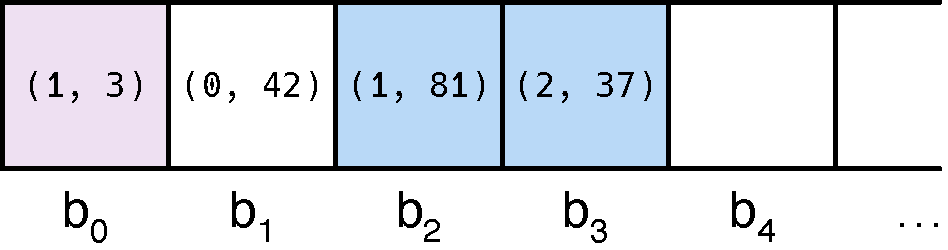
\includegraphics[width=\textwidth]{figs/sec3-5.pdf}
\end{minipage}
\end{enumerate}
%
Each of these states satisfies the key-value store's crash-consistency predicate $\consistent{d}$
defined in \cref{depsynth:s:overview},
as in each case the superblock's \texttt{head} and \texttt{tail} pointers
refer only to log blocks that are also on disk.
Some states result in data loss after the crash---%
for example, neither key can be retrieved from crash state \ref{sec:problem:loststate} above, as the superblock is empty---%
but these states are still consistent
(i.e., they satisfy the log's representation invariant).
This set of two rules therefore makes the \texttt{SingleEntry_TwoAppend} litmus test crash consistent according to \cref{def:crash-consistent}.

If the second rule $\deprule{\textsf{superblock}}{\textsf{superblock}}{>}$ was excluded,
the rule set with one remaining rule allows 2 additional crash states:
%
\begin{enumerate}[resume,label={\raisebox{3\baselineskip}[0pt][0pt]{(\arabic*)}},ref=(\arabic*)]
\item 
\begin{minipage}[b]{0.5\textwidth}
$[s_1 = \top, s_2 = \bot, s_3 = \top, s_4 = \top]$\\
(the first log block, second log block, and second superblock write are on disk) \\
\end{minipage}\quad%
\begin{minipage}{0.4\textwidth}
\vspace{-4em}
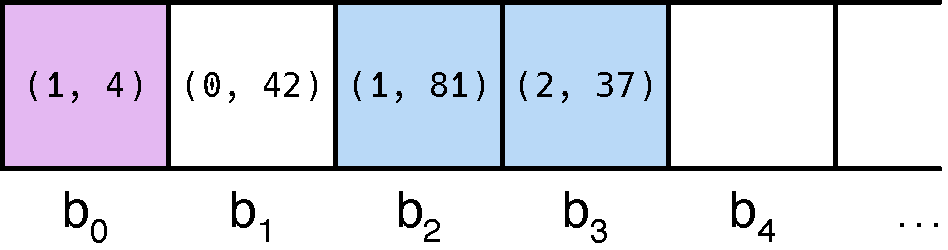
\includegraphics[width=\textwidth]{figs/sec3-6.pdf}
\end{minipage}
\label{sec:problem:goodstate}

\item 
\begin{minipage}[b]{0.5\textwidth}
$[s_1 = \bot, s_2 = \bot, s_3 = \top, s_4 = \top]$\\
(the second log block and second superblock write are on disk) \\
\end{minipage}\quad%
\begin{minipage}{0.4\textwidth}
\vspace{-4em}
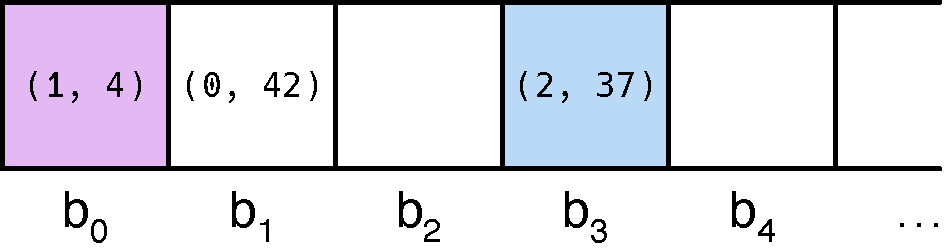
\includegraphics[width=\textwidth]{figs/sec3-7.pdf}
\end{minipage}
\label{sec:problem:badstate}
\end{enumerate}
%
\vspace{-1.5em}
State \ref{sec:problem:goodstate} satisfies the crash-consistency predicate despite losing the first superblock write,
as the second superblock write already contains the effects of the first one.
However, state \ref{sec:problem:badstate} violates the crash-consistency predicate:
the first log block is invalid,
but is included in the range between the superblock's \texttt{head} and \texttt{tail} pointers.
The set containing only the first rule therefore does not make \texttt{SingleEntry_TwoAppend} crash consistent.
\end{example}


\section{Dependency Rule Synthesis}\label{sec:alg}

This section describes the \depsynth synthesis algorithm,
which automatically generates a set of dependency rules
that are sufficient to guarantee crash consistency for a set of litmus tests.
It formalizes the dependency rule synthesis problem,
gives an overview of \depsynth's approach to synthesizing dependency rules,
and then presents the core \depsynth algorithm (\cref{fig:alg:depsynth}).

\subsection{Problem Statement}\label{sec:alg:problem}

\depsynth solves the problem of 
finding a \emph{single} set of dependency rules \ruleset
that makes every litmus test \test
in a set of tests \tests
crash consistent (\cref{def:crash-consistent}).
% As \cref{sec:problem:tests} discusses,
% the set of tests \tests of interest
% can be drawn from a number of sources,
% including hand-written tests
% and automated fuzzing or enumeration.
%
While \cref{def:crash-consistent} suffices to find a set of rules \ruleset
that guarantees crash consistency,
it does not rule out \emph{cyclic} solutions that cannot be executed on real hardware.
For example, consider a program $P$
where $\evaluate{P}{\sys} = [\texttt{write}(a_1, v_1, \langle n_1, t_1 \rangle), \texttt{write}(a_2, v_2, \langle n_2, t_2 \rangle)]$.
The set of rules $R = \{ \deprule{n_1}{n_2}{=}, \deprule{n_2}{n_1}{=} \}$
makes $P$ crash consistent.
These two rules do not admit any valid crash schedules
other than the trivial $\vec{s} = \vec{\top}$ and $\vec{s} = \vec{\bot}$ schedules,
as \cref{def:valid-schedule} forces $s_1 = s_2$.
In effect, crash consistency for $P$
requires both writes to happen ``at the same time''.
But on real disks the level of write atomicity is only a single data block,
so there is no way for both writes to happen at the same time.
To rule out cyclic solutions,
we follow the example of happens-before graphs~\cite{lamport:happens-before}
from distributed systems and memory consistency,
and require the set of synthesized dependency rules \ruleset to be \emph{acyclic}.\tighten

\subsection{The \depsynth Algorithm}

\begin{figure}
    \centering
    {\xsmall\begin{algorithmic}[1]
\Function{\depsynthalg}{\impl, \tests, \consist}
\State $\ruleset \gets \{\}$
\Loop
    \State $\test \gets \Call{NextTest}{\tests, \ruleset, \impl, \consist}$  \label{alg:depsynth:nexttest}
    \If{$\test = \bot$}  \Comment{\ruleset makes all tests in \tests crash consistent}
        \State \Return \ruleset
    \EndIf
    \State $\tests \gets \tests \setminus \test$
    \State $\ruleset' \gets \Call{\rulesfortest}{\test, \impl, \consist}$ \label{alg:depsynth:rulesone}
    \If{$\ruleset' = \bot$}
        \State \Return \UNSAT  \Comment{No rules can make \test crash consistent}
    \EndIf
    \State $\ruleset \gets \ruleset \cup \ruleset'$ \label{alg:depsynth:add}
    \If{$\neg \Call{Acyclic}{\ruleset}$}  \Comment{Fail if new rules create a cycle in the rule set}
        \State \Return \UNKNOWN  \label{alg:depsynth:resolve}
    \EndIf
\EndLoop
\EndFunction

\vspace{0.8em}

\Function{NextTest}{\tests, \ruleset, \impl, \consist}
    \For{$\test \in \tests$}
        \If{$\neg \Call{\crashconsistentalg}{\test, \ruleset, \impl, \consist}$}
            \State \Return \test
        \EndIf
    \EndFor
    \State \Return $\bot$
\EndFunction

\vspace{0.8em}

\Comment{Check Def.~\ref{def:crash-consistent} with an SMT solver}
\Function{\crashconsistentalg}{$\test = \langle P_\emph{initial}, P_\emph{main} \rangle$, \ruleset, \impl, \consist}  \label{alg:depsynth:cc}
    \State $d_\emph{initial} \gets \run{\evaluate{P_\emph{initial}}{\mathcal{O}}}{\vec{\top}}{d_0}$
    \State \Return $\forall \vec{s}.\ \valid{\vec{s}}{P_\emph{main}}{R} \Rightarrow \consistent{\run{\evaluate{P_\emph{main}}{\mathcal{O}}}{\vec{s}}{d_\emph{initial}}}$
\EndFunction

\algstore{depsynth}
\end{algorithmic}
}
    \caption{The \depsynth algorithm takes as input a storage system implementation $\sys$,
    a set of litmus tests \tests, and a crash-consistency predicate $\textrm{\emph{Consistent}}$,
    and returns an acyclic set of dependency rules that make all tests in \tests crash consistent (\cref{def:crash-consistent}).
    The search synthesizes dependency rules for one litmus test at a time.
    If the rules generated for two or more tests result in a cycle,
    this algorithm fails; \cref{sec:alg:cycles} discusses an extension for continuing 
    the search for an acyclic solution.}
    \label{fig:alg:depsynth}
\end{figure}

The \depsynthalg algorithm (\cref{fig:alg:depsynth})
takes as input a storage system implementation \sys,
a set of litmus tests \tests,
and a crash-consistency predicate $\emph{Consistent}$.
Given these inputs,
it synthesizes a set of dependency rules
that is acyclic and sufficient to make all tests \tests crash consistent.
% \depsynth delegates rule generation to
% a \textsc{RulesForTests} subprocedure (\cref{sec:alg:onetest})
% that takes as input a single test $\test$,
% evaluates it into a set of write operations $\{ w_i \}$,
% and searches for a minimal happens-before graph over those writes
% that is sufficient to ensure crash consistency.
% Once it identifies such a happens-before graph,
% it uses a simple syntactic approach
% to generalize it into a set of dependency rules
% that suffice to enforce the orderings in the graph.

\depsynthalg does not try to generate a sufficient set of dependency rules
for all tests in \tests at once,
since this would require a prohibitively expensive search
over large happens-before graphs.
Instead, it works incrementally:
at each iteration of its top-level loop,
\depsynthalg chooses a single test \test that is not made crash consistent
by the current candidate set of dependency rules (line~\ref{alg:depsynth:nexttest} in \cref{fig:alg:depsynth}), 
invokes the procedure \rulesfortest (\cref{sec:alg:onetest})
to synthesize dependency rules that make \test crash consistent,
and adds the new rules to the candidate set (line~\ref{alg:depsynth:add}).
Working incrementally reduces the number of litmus tests
for which \depsynthalg needs to synthesize rules;
for example, in \cref{sec:eval:shardstore} we show that only \shardstoretestsused of \shardstoreinputtests tests
were passed to \rulesfortest to synthesize a sufficient set of dependency rules
for a production key-value store.
This reduction relieves developers from being selective about the set of litmus tests they supply to \depsynth,
and makes it possible to, for example, use the output of a fuzzer or random test generator as input.

However, because the rules for each test are generated independently,
it is possible for the union of the generated rules to contain a cycle---%
even if the rules for each individual test do not---%
and so be an invalid solution (\cref{sec:alg:problem}).
The algorithm in \cref{fig:alg:depsynth}
returns \UNKNOWN if such a cycle is found.
We have not seen this failure mode occur for the storage systems we evaluated (\cref{sec:eval}),
but it is possible in principle.
In \cref{sec:alg:cycles}, we explain how to extend \depsynthalg
to recover from cycles by generalizing \rulesfortest to synthesize rules for multiple tests at once.

\depsynthalg delegates checking for crash consistency
to the procedure \crashconsistentalg (line~\ref{alg:depsynth:cc}), 
which takes as input a single litmus test
and a set of dependency rules,
and checks whether the rules make the test crash consistent
according to \cref{def:crash-consistent}.
This procedure uses symbolic evaluation of the storage system implementation \sys
to generate the logical encoding described in \cref{sec:problem:crashes},
and solves the resulting formulas using an off-the-shelf SMT solver~\cite{niemetz:boolector}.\tighten

\subsection{Synthesizing Dependency Rules with Happens-Before Graphs}\label{sec:alg:onetest}

\begin{figure}
    \centering
    {\xsmall\begin{algorithmic}[1]
\algrestore{depsynth}

\Function{\rulesfortest}{$\test = \langle P_\emph{initial}, P_\emph{main} \rangle$, \impl, \consist}
    \State $\wr \gets \{w\ | \ w \in \evaluate{P_\emph{main}}{\impl} \}$
    \State \Return $\Call{\phaseone}{\tests, [], \wr, \impl, \consist}$
\EndFunction

\vspace{0.8em}

\Function{\phaseone}{\test, \ord, \wr, \impl, \consist}  \Comment{Search for total orders over writes}  \label{fig:rules:phase1}
    \If{$\wr = \emptyset$}
        \State $\gr \gets \{ (\ord[i], \ord[j]) \ | \ 0 \leq i < j < |\ord| \}$
        \State \Return \Call{\phasetwo}{\tests, \gr, \impl, \consist}  \Comment{\gr is a total order; minimize it in Phase 2} \label{fig:rules:phase1tophase2}
    \EndIf
    \For{$w \in \wr$}
        \State $\ord' \gets \ord + [w]$
        \State $\wr' \gets \wr \setminus \{ w \}$
        \State $\gr \gets \{ (\ord[i], \ord[j]) \ | \ 0 \leq i < j < |\ord| \} \, \cup$ 
            \Statex $\hspace{6em}\{ (w_1, w_2) \ | \ w_1 \in \ord \land w_2 \in \wr \} \, \cup$ 
            \Statex $\hspace{6em}\{ (w_1, w_2) \ | \ w_1, w_2 \in \wr \}$  \label{fig:rules:phase1angelic}
         \If{$\neg \crashconsistentalg(\test, \Call{\rulesforgraph}{\gr}, \impl, \consist)$}  \label{fig:rules:phase1sufficient}
            \State \textbf{continue} \label{fig:rules:phase1continue}
        \EndIf
        \State $\ruleset \gets \Call{\phaseone}{\test, \ord', \wr', \impl, \consist}$
        \If{$\ruleset \neq \bot$}
            \State \Return \ruleset
        \EndIf
    \EndFor
    \State \Return $\bot$
\EndFunction

\algstore*{depsynth}
\end{algorithmic}
}
    \caption{The algorithm for generating sufficient dependency rules for a litmus test \test
    searches the space of happens-before graphs over the writes performed by \test.
    The first phase searches for total orders over the writes that are sufficient for crash consistency.
    Once such a total order is found, the second phase removes edges from it until the happens-before graph is minimal.}
    \label{fig:alg:rulesfortests}
\end{figure}

The core of the \depsynthalg algorithm is the
\rulesfortest procedure in \cref{fig:alg:rulesfortests},
which takes as input a litmus test \test,
a storage system implementation $\sys$,
and a crash-consistency predicate $\emph{Consistent}$,
and synthesizes a set of dependency rules
that makes \test crash consistent.
\rulesfortest frames the rule synthesis problem
as a search over \emph{happens-before graphs}~\cite{lamport:happens-before}
on the writes performed by the test.
An edge $(w_1, w_2)$ between two writes in a happens-before graph
says that write $w_1$ must persist to disk before write $w_2$.
Happens-before graphs and dependency rules have a natural correspondence:
if a happens-before graph includes an edge $(w_1, w_2)$,
a dependency rule $\deprule{n_2}{n_1}{p}$ that matches the writes' labels
is sufficient to enforce the required ordering.
\rulesfortest searches for a minimal, acyclic happens-before graph
that is sufficient to ensure crash consistency for \test,
and then syntactically generalizes that happens-before graph into a set of dependency rules.

\rulesfortest searches for a happens-before graph by first finding a \emph{total
order} on the writes that makes $T$ crash consistent (\phaseone), and then
searching for a minimal \emph{partial order} within this total order that is
both sufficient for crash consistency and yields an acyclic set of dependency
rules (\phasetwo). The algorithm is exhaustive: it tries all total orders and
all minimal partial orders within a total order, until it finds a solution or
fails because a solution does not exist.

\rulesfortest builds on the observation that crash consistency (\cref{def:crash-consistent})
is monotonic with respect to the subset relation on dependency rules---%
if a set of dependency rules \ruleset is not sufficient for crash consistency,
then no subset of \ruleset is sufficient either:
%
\begin{theorem}[Monotonicity of crash consistency]\label{thm:synthesis:monotonicity}
Let \test be a litmus test
and \ruleset a set of dependency rules for a storage system $\sys$.
If \ruleset does not make \test crash consistent (according to \cref{def:crash-consistent}),
then no subset $R' \subset R$ can make \test crash consistent.
\end{theorem}
\begin{proof}[Proof sketch]
If \ruleset does not make \test crash consistent,
there exists a valid crash schedule $\vec{s}$ (\cref{def:valid-schedule})
that does not satisfy the crash consistency predicate $\emph{Consistent}$.
By \cref{def:valid-schedule}, each rule in \ruleset only adds additional constraints on the possible valid crash schedules.
Removing a rule from \ruleset therefore only allows more valid crash schedules,
and so if $\vec{s}$ was a valid crash schedule for \ruleset, it is also a valid crash schedule for any subset of \ruleset.
\end{proof}
%
\noindent
\rulesfortest applies this property by checking crash consistency
for a happens-before graph \gr before exploring any subgraphs of \gr;
if \gr is not sufficient, then neither is any subgraph of \gr,
and so that branch of the search can be skipped.
% In contrast, a bottom-up search that tries to add new edges to \gr
% cannot be guided by this feedback,
% as knowing that a graph \gr is not sufficient does not give any information
% about whether a larger supergraph of \gr would provide crash consistency.

% As happens-before graphs are directed acyclic graphs,
% \rulesfortest splits the search for a minimal sufficient happens-before graph into two phases---%
% first searching for a candidate total order over the writes,
% and then shrinking that total order into a partial one that still ensures crash consistency.
% This phase split to accelerate the search;
% the first phase can remove many edges from the graph in a single step,
% and so can quickly rule out large portions of the search space,
% while the second phase works one edge at a time.

\paragraph{Total order search.}
\phaseone (line~\ref{fig:rules:phase1})
explores all possible total orders over the writes in \test
that are sufficient for crash consistency.
At each recursive call, the list \ord represents a total order over some of \test's writes,
and the set \wr contains all writes not yet added to that order.
\phaseone tries to add each write in \wr to the end of the total order.
Each time, it checks whether the new total order leads to a crash consistency violation (line~\ref{fig:rules:phase1sufficient})
and if so, prunes this branch of the search.
For \phaseone to be complete, 
this check must behave angellically for the writes in \wr that have not yet been added to the order---%
if there is \emph{any possible} set of dependency rules for the remaining writes that would succeed,
the check must succeed.
We make the check angelic by including every possible dependency rule for the remaining writes (line~\ref{fig:rules:phase1angelic}).
If the test cannot be made crash consistent even with every possible rule included,
then by \cref{thm:synthesis:monotonicity} no subset of those rules
(i.e., formed by completing the rest of the total order)
can succeed either, so the prefix is safe to prune.
\phaseone continues until every write has been added to the total order
and then moves to \phasetwo to further reduce the happens-before graph.\tighten

\paragraph{Partial order search.}
Starting from a happens-before graph \gr that reflects a total order over all writes in \test,
\phasetwo (line~\ref{fig:rules:phase2})
removes edges from the graph until it is minimal,
i.e., removing any further edges would violate crash consistency.
\phasetwo removes one edge at a time from the graph \gr (line~\ref{fig:rules:phase2remove}),
checks if the graph remains sufficient for crash consistency (line~\ref{fig:rules:phase2sufficient}),
and if so, recurses to remove more edges.
By greedily removing one edge at a time,
\phasetwo is guaranteed to find a minimal result,
and because \phasetwo considers removing every possible edge from \gr
(except those that cannot lead by solutions by \cref{thm:synthesis:monotonicity}),
it is complete---if an acyclic solution exists, \phasetwo will reach it.\tighten

\paragraph{Generating rules from happens-before graphs.}
The \rulesfortest search operates on happens-before graphs,
but its goal is to synthesize dependency rules (\cref{def:dependency-rule}).
The \rulesforgraph procedure (line~\ref{fig:rules:rulesforgraph})
bridges this gap
by taking as input a happens-before graph \gr
and returning a set of dependency rules \ruleset
that are sufficient to enforce the ordering requirements that \gr dictates.
\rulesforgraph uses a simple syntactic approach to generate a rule for each edge in \gr:
if $(w_1, w_2) \in \gr$,
where writes $w_1$ and $w_2$ have labels $l_1 = \langle n_1, t_1 \rangle$ and $l_2 = \langle n_2, t_2 \rangle$, respectively,
then it generates a rule of the form $\deprule{n_2}{n_1}{}$
(reversing the order because $G$ is a happens-before graph
but dependency rules are happens-\emph{after} edges).
To choose an epoch predicate for the generated rule,
we compare the two epochs $t_1$ and $t_2$
and select the predicate that would make the rule match the labels $l_1$ and $l_2$.\tighten

This approach can lead to rules that are too general,
as some rules it generates may only need to apply to certain individual epochs
but will instead apply to all epochs that match the predicate.
Overly general rules risk sacrificing performance
by preventing reordering or caching optimizations that would be safe.
However, this same generality also allows \textsc{RulesForTests} to avoid overfitting to the input litmus tests.
In \cref{sec:eval:shardstore} we show that generated rules generalize well in practice (i.e., are not overfit),
and that they filter out few additional schedules compared to expert-written rules.

\paragraph{Properties of \rulesfortest.}
The \rulesfortest algorithm is \emph{sound}:
all paths that return a solution are guarded by checks of crash consistency and of acyclicity,
and so satisfy the requirements of \cref{sec:alg:problem}.
\rulesfortest is also \emph{complete}:
each of \phaseone and \phasetwo are complete, as discussed above,
and so together form a complete search over the space of total orders. 
Every possible acyclic solution must be a subgraph of some total order,
since the transitive closure of edges in any happens-before graph is a (strict) partial order,
and so exploring all total orders suffices to reach any possible acyclic solution.
Finally, \rulesfortest is \emph{minimal},
in the sense that removing any rule from a returned set \ruleset
would violate crash consistency. 
\phasetwo continues removing edges from a candidate graph \gr
until \cref{thm:synthesis:monotonicity} says it cannot be made smaller,
and is therefore guaranteed to find a minimal happens-before graph. 
Every rule in \ruleset is justified by (at least) one edge in that graph,
and since dependency rules cannot overlap
(in \cref{def:dependency-rule}, the possible epoch predicates are disjoint),
removing any rule would incorrectly allow reordering of its corresponding edge(s).
%\todo{these are long sentences, perhaps we should just do three thms and proof sketches}

\begin{example}\label{sec:alg:example}
Consider running \rulesfortest for the simple log-structured key-value store
and \texttt{SingleEntry_TwoAppend} litmus test from \cref{s:overview}.
From \cref{sec:problem:example} we know that this test produces a set \wr of four writes:
%
\begin{align*}
    w_1 &= \texttt{write}(2, \texttt{to_block}((1, 81)), \langle \textsf{log}, 1 \rangle), \\
    w_2 &= \texttt{write}(0, \texttt{to_block}((1, 3)),  \langle \textsf{superblock}, 1 \rangle), \\
    w_3 &= \texttt{write}(3, \texttt{to_block}((2, 37)), \langle \textsf{log}, 2 \rangle), \\
    w_4 &= \texttt{write}(0, \texttt{to_block}((1, 4)),  \langle \textsf{superblock}, 2 \rangle)
\end{align*}
%
\phaseone first chooses the first write to add to the total order.
Suppose it chooses $w_2$.
This choice results in the following graph \gr at line~\ref{fig:rules:phase1angelic}
(shaded nodes are in \ord; white nodes are in \wr):
%
\begin{center}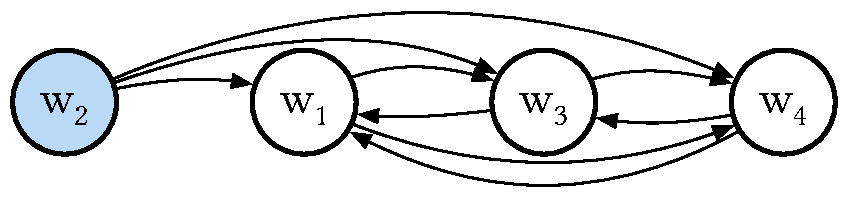
\includegraphics[width=0.5\textwidth]{figs/sec4-1.pdf}\end{center}
%
The check at line~\ref{fig:rules:phase1sufficient}
finds that this graph is not crash consistent: it allows a crash schedule where $w_2$ is on disk but no other writes are,
which violates the crash-consistency predicate as $w_2$ is a superblock write pointing to a log block that is not on disk.
\phaseone therefore continues (line~\ref{fig:rules:phase1continue}),
which prunes any total order that starts with $[w_2]$ from the search,
and chooses a next write to consider, say $w_3$.
The total order starting with $[w_3]$ does pass the crash consistency check,
so \phaseone recurses with $\ord = [w_3]$ and $\wr = \{w_1, w_2, w_4\}$.
In this recursive call,
suppose we again first choose $w_2$ to add to the total order.
This choice results in the following graph \gr:
%
\begin{center}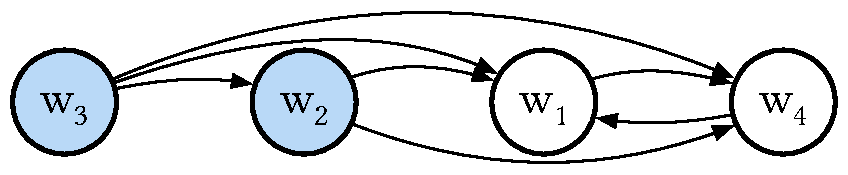
\includegraphics[width=0.5\textwidth]{figs/sec4-2.pdf}\end{center}
%
Again, line~\ref{fig:rules:phase1sufficient} finds that this graph is not crash consistent,
for the same reason as before (superblock write $w_2$ can be on disk when log write $w_1$ is not),
and so the search continues, pruning any total order that starts with $[w_3, w_2]$.
Suppose it next chooses $w_1$ to add to the total order.
This choice succeeds, making the recursive call with $\ord = [w_3, w_1]$ and $\wr = \{w_2, w_4\}$.
From here, any choice \phaseone makes will succeed.
Supposing it choses $w_2$ first,
\phaseone eventually reaches line~\ref{fig:rules:phase1tophase2} and continues to \phasetwo
with the following initial graph \gr:
%
\begin{center}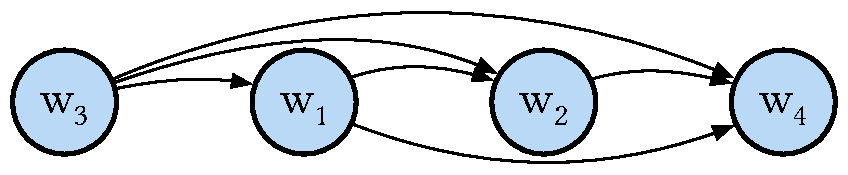
\includegraphics[width=0.5\textwidth]{figs/sec4-3.pdf}\end{center}

\phasetwo proceeds by trying to remove one edge at a time from \gr.
Suppose it first chooses to remove edge $(w_3, w_1)$,
and so recurses at line~\ref{fig:rules:phase2recurse} on the graph $\gr' = \gr \setminus \{(w_3, w_1)\}$.
This graph still ensures crash consistency at line~\ref{fig:rules:phase2sufficient},
as writing $w_1$ before $w_3$ does not affect consistency.
The recursion can continue twice more
by choosing and successfully removing edges $(w_3, w_2)$ and then $(w_1, w_4)$ as well,
eventually reaching line~\ref{fig:rules:phase2loop} with the following graph \gr (now with write labels shown):\tighten
%
\begin{center}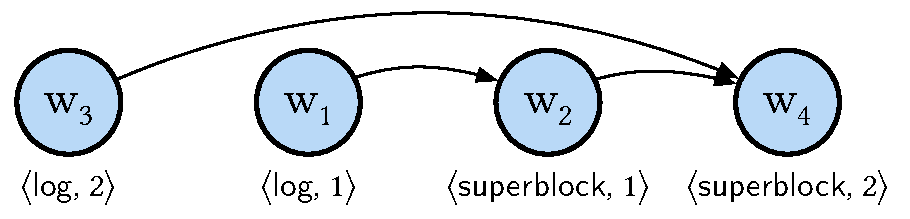
\includegraphics[width=0.5\textwidth]{figs/sec4-4.pdf}\end{center}
%
From here, the loop in \phasetwo now tries to remove each of the three remaining edges,
but each attempted $\gr'$ violates crash consistency and so returns $\bot$ from the next recursive call.
\phasetwo therefore exits the loop with the above graph \gr,
which we now know is minimal as no further edges can be removed.
Applying \rulesforgraph to \gr yields the two rules from \cref{s:overview}:
\begin{align*}
    \deprule{\textsf{superblock}&}{\textsf{log}}{=} & \text{ from edges } (w_3, w_4) \text{ and } (w_1, w_2) \\
    \deprule{\textsf{superblock}&}{\textsf{superblock}}{>} & \text{ from edge } (w_2, w_4).
\end{align*}
\end{example}


\subsection{Resolving Cycles in Dependency Rules}\label{sec:alg:cycles}

% \begin{figure}
%     \centering
%     {\xsmall\newcommand{\impl}{\ensuremath{\mathcal{O}}\xspace}
\newcommand{\test}{\ensuremath{T}\xspace}
\newcommand{\tests}{\ensuremath{\mathcal{T}}\xspace}
\newcommand{\consist}{\ensuremath{\emph{Consistent}}\xspace}
\newcommand{\rulemap}{\ensuremath{\mathcal{R}}\xspace}
\newcommand{\ruleset}{\ensuremath{R}\xspace}
% \newcommand{\writesused}{\ensuremath{W_U}\xspace}
% \newcommand{\writesleft}{\ensuremath{W_R}\xspace}
\renewcommand{\wr}{\ensuremath{W}\xspace}
\newcommand{\ord}{\ensuremath{V}\xspace}
\newcommand{\gr}{\ensuremath{G}\xspace}
\newcommand{\comp}{\ensuremath{C}\xspace}

\begin{algorithmic}[1]
\algrestore{depsynth}

\Function{ResolveCycle}{\rulemap, \impl, \consist}
    \State $C \gets \Call{GetCycle}{\cup_{(T' \mapsto R) \in \rulemap} R}$  \Comment{Identify rules $C \subseteq R$ that participate in the cycle}
    \State $\tests' \gets \{ T \ | \ (T \mapsto R) \in \rulemap \land T \in C \}$  \Comment{Collect the tests that generated rules in $C$}
    \State \Return \Call{RulesForTests}{\tests', \impl, \consist}
\EndFunction

\end{algorithmic}}
%     \caption{The algorithm for resolving cycles in a set of generated dependency rules.
%     \textsc{ResolveCycles} takes as input a mapping from litmus tests to sets of dependency rules
%     such that the union of the sets contains a cycle. It returns a new mapping from the same set of
%     litmus tests to sets of dependency rules that no longer contains a cycle.}
%     \label{fig:alg:resolvecycles}
% \end{figure}

The top-level \depsynthalg algorithm generates rules for each litmus test independently.
Even though the rules generated for each test are guaranteed to be acyclic,
it is possible for the \emph{union} of those rules to contain a cycle,
and so violate the requirements of \cref{sec:alg:problem}.
In practice, we have not seen this happen for the storage systems we evaluate in \cref{sec:eval},
and so the version of \depsynthalg presented in \cref{fig:alg:depsynth} fails if the synthesized rules contain a cycle.

To handle cyclic rules,
\rulesfortest can be extended to support synthesizing rules for multiple litmus tests at once.
This extension adds the writes from \emph{all} the tests into the set of writes \wr,
searches for a total order over that entire set in \phaseone,
and then searches for a minimal happens-before graph over the entire set in \phasetwo.
Edges between writes from different tests
cannot influence the crash consistency of individual tests
(in \cref{def:valid-schedule} they will just lead to spurious additional implications),
and they will eventually be removed by \phasetwo,
creating a forest of disjoint happens-before graphs.
\phasetwo is therefore guaranteed to return an acyclic set of dependency rules
for all the tests it was provided.

In the limit, \depsynthalg could just invoke \rulesfortest with its entire input set \tests,
but this would be prohibitively expensive for any non-trivial set of tests.
Instead, our implementation resolves cycles in \depsynthalg
by identifying which individual litmus tests caused the cycle
(i.e., which tests the rules in the cycle were generated from),
and passes only that subset of tests to the extended \rulesfortest.


% 

\section{Solving the \MiniCompiler Synthesis Problem}
\label{s:algorithm}

This section presents our approach to solving the \minicompiler synthesis
problem defined in \autoref{s:problem}. We employ syntax-guided
synthesis~\cite{solar-lezama:sketch} to search for an implementation of a
\minicompiler in a space of candidate programs. Our core contribution is an
effective way to structure this space using a \emph{compiler metasketch}. This
section presents our algorithm for generating compiler metasketches, describes
its key subroutines and optimizations, and shows how to solve the resulting
sketches with an off-the-shelf synthesis engine.\tighten
%, and highlights key details of our implementation of \jitsynth.\tighten


\subsection{Generating Compiler Metasketches}

\jitsynth synthesizes \minicompilers by generating and solving
\emph{metasketches}~\cite{bornholt:synapse}. A metasketch describes a space of
candidate programs using an ordered set of syntactic templates or
\emph{sketches}~\cite{solar-lezama:sketch}. These sketches take the form of
programs with missing expressions or \emph{holes}, where each hole describes a
finite set of candidate completions. \jitsynth sketches are expressed in a
\emph{host language} \host that serves both as the implementation language for
\minicompilers and the specification language for ARMs. \jitsynth expects the
host to provide a synthesizer for completing sketches and a symbolic evaluator
for reducing ARM semantics to SMT constraints. \jitsynth uses these tools to
generate optimized metasketches for \minicompilers, which we call \emph{compiler
metasketches}.\tighten

\autoref{alg:compiler-metasketch-generator} shows our algorithm for generating
compiler metasketches. The algorithm, \CMS, takes as input an abstract source
instruction $\iota$ for a source machine $\arm_S$, a target machine $\arm_T$,
and a state mapping \Map from $\arm_S$ to $\arm_T$. Given these inputs, it
lazily enumerates an infinite set of \emph{compiler sketches} that collectively
represent the space of all straight-line bitvector programs from $\prog{\iota}$
to $\mathid{List}(\prog{\mathcal{I}_T})$. In particular, each compiler sketch
consists of $k$ target \emph{instruction holes}, constructed from {field holes}
that denote bitvector expressions (over the fields of $\iota$) of depth $d$ or
less. For each length $k$ and depth $d$, the \CMS loop generates three kinds of
compiler sketches: the \emph{pre-load}, the \emph{read-write}, and the
\emph{naive} sketch. The naive sketch (\autoref{s:algorithm:naive}) is the most
general, consisting of all candidate \minicompilers of length $k$ and depth $d$.
But it also scales poorly, so \CMS first yields the pre-load
(\autoref{s:algorithm:pld}) and  read-write (\autoref{s:algorithm:rw}) sketches.
As we will see later, these sketches describe a subset of the programs in the
naive sketch, and they are designed to prioritize exploring small parts of the
search space that are likely to contain a correct \minicompiler for $\iota$, if
one exists.

\begin{figure}[t]
\begin{algorithmic}[1] 
  \Function{CMS}
    {$\iota, \arm_S, \arm_T, \Map$} \Comment{$\iota\in\mathcal{I}_S, \arm_S = (\mathcal{I}_S, \ldots)$}
    \For{$n\in\mathbb{Z}^+$} \Comment{Lazily enumerates all compiler sketches}
      \For{$k \in [1, n], d = n-k$} \Comment{of length $k$ and depth $d$,}
        \State \textbf{yield} $\LCS(k,d,\iota,\arm_S,\arm_T,\Map)$ \Comment{yielding the pre-load sketch first,}
        \State \textbf{yield} $\RW(k,d,\iota,\arm_S,\arm_T,\Map)$ \Comment{read-write sketch next, and}
        \State \textbf{yield} $\Naive(k,d,\iota,\arm_S,\arm_T,\Map)$ \Comment{the most general sketch last.}
      \EndFor
    \EndFor
  \EndFunction
\end{algorithmic}
\caption{Compiler metasketch for the abstract source instruction
$\iota$, source machine $\arm_S$, target machine $\arm_T$, and state mapping
$\mathcal{M}$ from $\arm_S$ to
$\arm_T$.\tighten}\label{alg:compiler-metasketch-generator}
\end{figure}

\subsection{Generating Naive Sketches}\label{s:algorithm:naive}

The most general sketch we consider, $\Naive(k,d,\iota,\arm_S,\arm_T,\Map)$, is
shown in \autoref{fig:naive-sketch}. This sketch consists of $k$ instruction
holes that can be filled with any instruction from $\mathcal{I}_T$. An
instruction hole chooses between expressions of the form $(\mathit{op}_T, H)$,
where $\mathit{op}_T$ is a target opcode, and $H$ specifies the field holes for
that opcode. Each field hole is a bitvector expression (of depth $d$) over the
fields of the input source instruction and arbitrary bitvector constants. This
lets target instructions use the immediates and registers (modulo \Map) of the
source instruction, as well as arbitrary constant values and register names.
Letting field holes include constant register names allows the synthesized
\minicompilers to use target registers unmapped by \Map as temporary, or
scratch, storage. In essence, the naive sketch describes all straight-line
compiler programs that can make free use of standard C arithmetic and bitwise
operators, as well as scratch registers.\tighten 

The space of such programs is intractably large, however, even for small inputs.
For instance, it includes at least $2^{350}$ programs of length $k=5$ and depth
$d\leq 3$ for the toy example from \autoref{jitsynth:s:overview}. \jitsynth therefore
employs two effective heuristics to direct the exploration of this space toward
the most promising candidates first, as defined by the read-write and pre-load
sketches.\tighten 

\begin{figure}
\begin{algorithmic}[1] 
  \Function{Naive}
    {$k, d, \iota , \arm_S, \arm_T, \Map$} \Comment{$\iota\in\mathcal{I}_S, \arm_S = (\mathcal{I}_S, \ldots)$}
    \State $(\mathid{op}, \mathcal{F}) \gets \iota$, $(\mathid{I}_T, \ldots) \gets \arm_T$ \Comment{Source instruction, target instructions.}
    \State $p \gets \mathid{FreshId}()$ \Comment{Identifier for the compiler's input.}
    \State $\mathid{body}\gets []$  \Comment{The body of the compiler is a sequence}
    \For{$0 \leq i < k$} \Comment{of $k$ target instruction holes.}
      \State $I \gets \{\}$  \Comment{The set $I$ of choices for a target instruction hole}
      \For{$(\mathid{op}_T, \mathcal{F}_T)\in\mathcal{I}_T$} \Comment{includes all instructions from $\mathcal{I}_T$.} \label{li:instruction-hole}
        \State $E \gets \{\mathid{Expr}(p.f, \Map) \,|\, f\in\mathid{dom}(\mathcal{F})\}$ \Comment{Any source field can appear in}
        \State $H \gets \{ f\mapsto \mathid{Field}(\mathcal{F}_T(f),d,E) \,|\, f\in\mathid{dom}(\mathcal{F}_T)\} $ \Comment{a target field hole, and}\label{li:field-holes}
        \State $I\gets I \cup \{ \mathit{Expr}((\mathid{op}_T, H), \Map) \}$ \Comment{any constant register or value.}
      \EndFor
      \State $\mathid{body} \gets \mathid{body} \cdot [\mathid{Choose}(I)]$ \Comment{Append a hole over $I$ to the body.}
    \EndFor
    \State \Return $\mathid{Expr}((\lambda p\in\prog{\iota}\, .\, \mathid{body}),\Map)$ \Comment{A \minicompiler sketch for $\iota$.}
  \EndFunction
\end{algorithmic}
\caption{Naive sketch of length $k$ and maximum depth $d$ for $\iota$, $\arm_S$,
$\arm_T$, and \Map. Here, $\mathid{Expr}$ creates an expression in the host language, 
using \Map to map from source to target register names and memory addresses;
$\mathid{Choose}(E)$ is a hole that chooses an expression from the set $E$; and
$\mathid{Field}(\tau,d,E)$ is a hole for a bitvector expression of type
$\tau$ and maximum depth $d$, constructed from arbitrary bitvector constants and
expressions $E$.\tighten}\label{fig:naive-sketch}
\end{figure}

%bvand bvadd bvshl bvor bvxor bvlshr bvashr

\subsection{Generating Read-Write Sketches}\label{s:algorithm:rw} 

The read-write sketch, $\RW(k, d, \iota, \arm_S, \arm_T, \Map)$, is based on the
observation that many practical source and target languages provide similar
functionality, so a source instruction $\iota$ can often be emulated with target
instructions that access the same parts of the state as $\iota$. For example,
the \cc{addi32} instruction from eBPF reads and writes only registers (not,
e.g., memory), and it can be emulated with RISC-V instructions that also touch
only registers (\autoref{jitsynth:s:overview}). Moreover, note that the semantics of
\cc{addi32} ignores the values of its $\mathid{src}$ and $\mathid{off}$
fields, and that the target RISC-V instructions do the same. Based on these
observations, our optimized sketch for \cc{addi32} would therefore consists of
instruction holes that allow only register-register instructions, with field
holes that exclude $\mathid{src}$ and $\mathid{off}$. We first formalize this
intuition with the notion of \emph{read and write sets}, and then describe how \jitsynth
applies such sets to create \RW sketches.\tighten

\paragraph{Read and write sets.} 
Read and write sets provide a compact way to summarize the semantics of an
abstract instruction $\iota$. This summary consists of a set of \emph{state
labels}, where a state label is one of $L_\regs$, $L_\mem$, and $L_\pc$
(\autoref{def:state-labels}). Each label in a summary set represents a state
component (registers, memory, or the program counter) that a concrete instance
of $\iota$ may read or write during some execution. We compute three such sets
of labels for every $\iota$: the read set $\Read{\iota}$, the write set
$\Write{\iota}$, and the write set $\Write{\iota, f}$ for each field $f$ of
$\iota$. \autoref{fig:rw-sets} shows these sets for the toy eBPF and RISC-V
instructions.\tighten



\begin{figure}\centering
  {\small
  \begin{tabular}{llll}
    \toprule
    $\iota$ & $\Read{\iota}$ & $\Write{\iota}$ & $\Write{\iota, \mathid{field}}$ \\
    \midrule
    \cc{addi32} & $\{L_\regs\}$ & $\{L_\regs\}$ & $\mathid{imm}$: $\{L_\regs\}$; $\mathid{off}$: $\emptyset$; $\mathid{src}$: $\emptyset$; $\mathid{dst}$: $\{L_\regs\}$ \\
    \cc{lui} & $\{L_\regs\}$ & $\{L_\regs\}$ & $\mathid{rd}$: $\{L_\regs\}$; $\mathid{imm20}$: $\{L_\regs\}$\\
    \cc{sb} & $\{L_\regs\}$ & $\{L_\mem\}$ & $\mathid{rs1}$: $\{L_\mem\}$; $\mathid{rs2}$: $\{L_\mem\}$; $\mathid{imm12}$: $\{L_\mem\}$ \\
    \bottomrule\end{tabular}
  }

\caption{Read and write sets for the \cc{addi32}, \cc{lui}, and \cc{sb} instructions from \autoref{fig:lang-instrs}.}\label{fig:rw-sets}
\end{figure}

The read set $\Read{\iota}$ specifies which components of the input state may
affect the execution of $\iota$ (\autoref{def:read-set}). For example, if
$\Read{\iota}$ includes $L_\regs$, then some concrete instance of $\iota$
produces different output states when executed on two input states that differ
only in register values. 
% More generally, $L_n \in \Read{\iota}$ means that the behavior of $\iota$ depends on the values read from the component $n$.\tighten
%
The write set $\Write{\iota}$ specifies which components of the output state may
be affected by executing $\iota$ (\autoref{def:write-set}). In particular, if
$\Write{\iota}$ includes $L_\regs$ (or $L_\mem$), then executing some concrete
instance of $\iota$ on an input state produces an output state with different
register (or memory) values. The inclusion of $L_\pc$ is based on a separate
condition, designed to distinguish jump instructions from fall-through
instructions. Both kinds of instructions change the program counter, but
fall-through instructions always change it in the same way. So,
$L_\pc\in\Write{\iota}$ if two instances of $\iota$ can write different values
to the program counter.
%
Finally, the field write set, $\Write{\iota, f}$, specifies the parts of the
output state are affected by the value of the field $f$; $L_n \in
\Write{\iota, f}$ means that two instances of $\iota$ that differ only in $f$
can produce different outputs when applied to the same input state.\tighten

\jitsynth computes all read and write sets from their definitions, by using the
host symbolic evaluator to reduce the reasoning about instruction semantics to
SMT queries. This reduction is possible because we assume that all ARM
interpreters are self-finitizing, as discussed in \autoref{jitsynth:s:overview}.

\begin{definition}[State Labels]\label{def:state-labels} 
  A \emph{state label} is an identifier $L_n$ where $n$ is a state component,
  i.e., $n\in \{\regs,\mem,\pc\}$. We write $N$ for the set of all state
  components, and $\mathcal{L}$ for the set of all state labels. We also use
  state labels to access the corresponding state components:
  $\Get{L_n}{\sigma} = n(\sigma)$ for all $n\in N$.
\end{definition}

\begin{definition}[Read Set]\label{def:read-set}
  Let $\iota\in\mathcal{I}$ be an abstract instruction in $(\mathcal{I},
  \Sigma, \mathcal{T}, \Phi)$. The \textup{read set} of $\iota$,
  $\Read{\iota}$, is the set of all state labels $L_n\in\mathcal{L}$ such that 
  $
    \exists p\in\prog{\iota}.\, 
    \exists L_w \in\Write{\iota}.\,
    \exists \sigma_a, \sigma_b \in\Sigma.\,
    (\Get{L_n}{\sigma_a} \neq \Get{L_n}{\sigma_b} \wedge 
    (\bigwedge_{m\in N \setminus \{ n \}} \Get{L_m}{\sigma_a} = \Get{L_m}{\sigma_b}) \wedge
    \Get{L_w}{\mathcal{T}(p,\sigma_a)} \neq \Get{L_w}{\mathcal{T}(p,\sigma_b)}.
  $\tighten
\end{definition}

\begin{definition}[Write Set]\label{def:write-set}
  Let $\iota\in\mathcal{I}$ be an abstract instruction in $(\mathcal{I}, \Sigma,
  \mathcal{T}, \Phi)$. The \textup{write set} of $\iota$, $\Write{\iota}$,
  includes the state label $L_n \in \{ L_\regs, L_\mem \}$ iff 
  $
    \exists p\in\prog{\iota}.\, 
    \exists \sigma \in\Sigma.\, 
    \Get{L_n}{\sigma} \neq \Get{L_n}{\mathcal{T}(p,\sigma)}
  $, 
  and it includes the state label $L_\pc$ iff 
  $
    \exists p_a, p_b\in\prog{\iota}.\, 
    \exists \sigma \in\Sigma.\,
    \Get{L_\pc}{\mathcal{T}(p_a,\sigma)} \neq \Get{L_\pc}{\mathcal{T}(p_b,\sigma)}.
  $\tighten
\end{definition}

\begin{definition}[Field Write Set]\label{def:field-set}
  Let $f$ be a field of an abstract instruction $\iota =
  (\mathid{op},\mathcal{F})$ in $(\mathcal{I}, \Sigma, \mathcal{T}, \Phi)$. The
  \textup{write set} of $\iota$ and $f$, $\Write{\iota, f}$, includes
  the state label $L_n \in \mathcal{L}$ iff 
  $
    \exists p_a, p_b\in\prog{\iota}.\, 
    \exists \sigma \in\Sigma.\ 
    (p_a.f \neq p_b.f) \wedge
    (\bigwedge_{g\in\mathid{dom}(\mathcal{F})\setminus\{f\}} p_a.g = p_b.g) \wedge
    \Get{L_n}{\mathcal{T}(p_a,\sigma)} \neq \Get{L_n}{\mathcal{T}(p_b,\sigma)}
  $, where $p.f$ denotes $F(f)$ for $p = (op, F)$. 
\end{definition}



% \begin{example}\label{ex:rw-sets}
%   \jitsynth computes the following read and write sets of $\iota = \cc{addi32}$:
%   $\Read{\iota} = \Write{\iota} = \Write{\iota, \mathid{dst}} = \Write{\iota,
%   \mathid{imm}} = \{L_\regs\}$, and $\Write{\iota, \mathid{src}} \\ = \Write{\iota,
%   \mathid{offset}} = \{\}$. The read and write sets for $\cc{lui}$ and its
%   fields are also $\{ L_\regs \}$, while for $\iota = \cc{sb}$, we get
%   $\Read{\iota}  = \{L_\regs \}$ and $\Write{\iota}  = \Write{\iota, f} =
%   \{L_\mem \}$ for each field $f$ of \cc{sb}.\tighten
% \end{example}



\paragraph{Using read and write sets.}  


Given the read and write sets for a source instruction $\iota$ and target
instructions $\mathcal{I}_T$, \jitsynth generates the \RW sketch of length $k$
and depth $d$ by modifying the \Naive algorithm (\autoref{fig:naive-sketch}) as
follows. First, it restricts each target instruction hole (line
\ref{li:instruction-hole}) to choose an instruction $\iota_T\in\mathcal{I}_T$
with the same read and write sets as $\iota$, i.e., $\Read{\iota} =
\Read{\iota_T}$ and  $\Write{\iota} = \Write{\iota_T}$. Second, it restricts the
target field holes (line \ref{li:field-holes}) to use the source fields with the
matching field write set, i.e., the hole for a target field $f_T$ uses the
source field $f$ when $\Write{\iota_T, f_t} = \Write{\iota, f}$. For example,
given the sets from \autoref{fig:rw-sets}, the \RW instruction holes for
\cc{addi32} exclude \cc{sb} but include \cc{lui}, and the field holes for
\cc{lui} use only the $\mathid{dst}$ and $\mathid{imm}$ source fields. More
generally, the \RW sketch for \cc{addi32} consists of register-register
instructions over $\mathid{dst}$ and $\mathid{imm}$, as intended. This sketch
includes $2^{290}$ programs of length $k=5$ and depth $d\leq 3$, resulting in a
$2^{60}$ fold reduction in the size of the search space compared to the \Naive
sketch of the same length and depth. 

% These restrictions capture the hypothesis that $\iota$ can be compiled to
% $\mathcal{I}_T$ instructions that manipulate state in the same way as $\iota$.
% This intuition, in turn, assumes that the states of the source and target
% machines are related by a state mapping (\autoref{def:state-equiv}) rather than
% an arbitrary equivalence relation.


\subsection{Generating Pre-Load Sketches}\label{s:algorithm:pld} 

The pre-load sketch, $\LCS(k, d, \iota, \arm_S, \arm_T, \Map)$, is based on the
observation that hand-written JITs use macros or subroutines to generate
frequently used target instruction sequences. For example, compiling a source
instruction with immediate fields often involves loading the immediates into
scratch registers, and hand-written JITs include a subroutine that generates the
target instructions for performing these loads. The pre-load sketch shown in
\autoref{fig:lcs-sketch} mimics this structure.\tighten 


In particular, \LCS generates a sequence of $m$ concrete instructions that load
the (used) immediate fields of $\iota$, followed by a sequence of $k-m$
instruction holes. The instruction holes can refer to both the source registers
(if any) and the scratch registers (via the arbitrary bitvector constants
included in the \emph{Field} holes). The function
$\mathid{Load}(\mathid{Expr}(p.f), \arm_T, \Map)$ returns a sequence of target
instructions that load the immediate $p.f$ into an unused scratch register. This
function itself is synthesized by \jitsynth using a variant of the \RW
sketch.\tighten 

As an example, the pre-load sketch for \cc{addi32} consists of two $\mathid{Load}$
instructions (\cc{lui} and \cc{addiw} in the generated C code) and $k-2$
instruction holes.  The holes choose among register-register instructions in toy
RISC-V, and they can refer to the $\mathid{dst}$ register of \cc{addi32}, as
well as any scratch register. The resulting sketch includes $2^{100}$ programs
of length $k = 5$ and depth $d\leq 3$, providing a $2^{190}$ fold reduction in
the size of the search space compared to the \RW sketch.\tighten

\begin{figure}[H]
  \begin{algorithmic}[1] 
    \Function{PLD}
      {$k, d, \iota, \arm_S, \arm_T, \Map$}\Comment{$\iota\in\mathcal{I}_S, \arm_S = (\mathcal{I}_S, \ldots)$}
      \State $(\mathid{op}, \mathcal{F}) \gets \iota$, $(\mathid{I}_T, \ldots) \gets \arm_T$ \Comment{Source instruction, target instructions.}
      \State $p \gets \mathid{FreshId}()$ \Comment{Identifier for the compiler's input source instruction.}
      \State $\mathid{body}\gets []$  \Comment{The body of the compiler is a sequence with 2 parts:}
      \State $\mathid{imm} \gets \{ f \,|\, \mathcal{F}(f) = \BV{k} \text{ and } \Write{\iota,f} \neq \emptyset \}$ \Comment{(1) Load each relevant}
      \For{$f \in \mathid{imm}$} \Comment{source immediate into a free scratch register}
        \State $\mathid{body}\gets\mathid{body}\cdot \mathid{Load}(\mathid{Expr}(p.f), \arm_T, \Map)$ \Comment{using the load pseudoinstruction.}
      \EndFor
      % \If{$L_\pc\in\Read{\iota}$} \Comment{If $\iota$ reads the PC, load it into a free scratch register}
      %   \State $\mathid{body}\gets\mathid{body}\cdot \mathid{LoadPC}(\arm_T, \Map)$ \Comment{using the load PC pseudoinstruction.}
      % \EndIf
      \State $m \gets |\mathid{body}|$ \Comment{Let $m$ be the length of the load sequence.}
      \If{$m\geq k$ or $m = 0$} \Return $\bot$ \Comment{Return the empty sketch if $m\not\in (0..k)$.}
      \EndIf
      \For{$m \leq i < k$} \Comment{(2) Create $k-m$ target instruction holes, where the set}
        \State $I \gets \{\}$  \Comment{$I$ of choices for a target instruction hole includes}
        \For{$\iota_T\in\mathcal{I}_T, \iota_T = (\mathid{op}_T, \mathcal{F}_T)$} \Comment{all instructions from $\mathcal{I}_T$ that read-write}  
         \State $\mathid{rw}_T \gets  \Read{\iota_T} \times \Write{\iota_T}$ \Comment{the same state as $\iota$ or just registers.}
          \If{$\mathid{rw}_T = \Read{\iota} \times \Write{\iota}$ or $\mathid{rw}_T \subseteq \{L_\regs\} \times \{L_\regs\}$ }
            \State $\mathid{regs} \gets \{ f \,|\, \mathcal{F}(f) = \Reg \text{ and } \Write{\iota,f} \neq \emptyset \}$ \Comment{Any relevant}
            \State $E \gets \{\mathid{Expr}(p.f, \Map) \,|\, f\in\mathid{regs}\}$ \Comment{source register can appear in}
            \State $H \gets \{ f\mapsto \mathid{Field}(\mathcal{F}_T(f),d,E) \,|\, f\in\mathid{dom}(\mathcal{F}_T)\} $ \Comment{a target field hole,} 
            \State $I\gets I \cup \{ \mathit{Expr}((\mathid{op}_T, H),\Map) \}$ \Comment{and any constant register or value.}
          \EndIf
        \EndFor
        \State $\mathid{body} \gets \mathid{body} \cdot [\mathid{Choose}(I)]$ \Comment{Append a hole over $I$ to the body.}
      \EndFor
      % \If{$L_\pc\in\Write{\iota}$} \Comment{(3) If $\iota$ writes the PC, move a scratch register value}
      %   \State $\mathid{body}\gets\mathid{body}\cdot \mathid{StorePC}(\arm_T, \Map)$ \Comment{into the PC using a pseudoinstruction.}
      % \EndIf
      \State \Return $\mathid{Expr}((\lambda p\in\prog{\iota}\, .\, \mathid{body}),\Map)$ \Comment{A \minicompiler sketch for $\iota$.}
    \EndFunction
  \end{algorithmic}
  \caption{Pre-load sketch of length $k$ and maximum depth $d$ for $\iota$,
  $\arm_S$, $\arm_T$, and \Map. The $\mathid{Load}(E, \arm_T, \Map)$ function
  returns a sequence of target instructions that load the immediate value
  described by the expression $E$ into an unused scratch register; see
  \autoref{fig:naive-sketch} for descriptions of other helper
  functions.\tighten}\label{fig:lcs-sketch}
\end{figure}


\subsection{Solving Compiler Metasketches}\label{s:algorithm:solving}

\jitsynth solves the metasketch $\CMS(\iota, \arm_S, \arm_T, \Map)$ by applying
the host synthesizer to each of the generated sketches in turn until a
\minicompiler is found. If no \minicompiler exists in the search space, this
synthesis process runs forever. To check if a sketch $\mathcal{S}$ contains a
\minicompiler, \jitsynth would ideally ask the host synthesizer to solve the
following query, derived from Definitions \ref{def:mini-compiler}--\ref{def:state-equiv}: 
{\small
\[
    \exists C\in\mathcal{S} . \ 
    \forall \sigma_S\in\Sigma_S,\ \sigma_T\in\Sigma_T,\ p\in\prog{\iota}. \\ 
      \sigma_S \cong_{\Map} \sigma_T \Rightarrow
      \arm_S(p, \sigma_S) \cong_{\Map} \arm_T(C(p), \sigma_T)
\]}%
But recall that the state equivalence check $\cong_{\Map}$ involves universally
quantified formulas over memory addresses and register names. In principle,
these innermost quantifiers are not problematic because they range over finite
domains (bitvectors) so the formula remains decidable. In practice, however,
they lead to intractable SMT queries. We therefore solve a stronger soundness
query (\autoref{def:strong-mini-compiler}) that pulls these quantifiers out to
obtain the standard $\exists\forall$ formula with a quantifier-free body. The  
resulting formula can be solved with CEGIS~\cite{solar-lezama:sketch}, without 
requiring the underlying SMT solver to reason about quantifiers.

\begin{definition}[Strongly Sound \MiniCompiler]\label{def:strong-mini-compiler}
  Let $\arm_S = (\mathcal{I}_S, \Sigma_S, \mathcal{T}_S, \Phi_S)$ and $\arm_T =
  (\mathcal{I}_T, \Sigma_T, \mathcal{T}_T, \Phi_T)$ be two abstract register
  machines, $\cong_{\Map}$ an injective state equivalence relation on their
  states $\Sigma_S$ and $\Sigma_T$, and $C: \prog{\iota} \rightarrow
  \mathid{List}(\prog{\mathcal{I}_T})$ a function for some
  $\iota\in\mathcal{I}_S$. We say that $C$ is a \textup{strongly sound
  \minicompiler} for $\iota_{\Map}$ with respect to $\cong$ iff
  \begin{align*}\small
    & \forall \sigma_S\in\Sigma_S,\ \sigma_T\in\Sigma_T,\ p\in\prog{\iota}, \
    a\in\mathid{dom}(\mem(\sigma_S)),\ r\in\mathid{dom}(\regs(\sigma_S)). \\ 
    & \sigma_S \cong_{\Map,a,r} \sigma_T \Rightarrow
       \arm_S(p, \sigma_S) \cong_{\Map,a,r} \arm_T(C(p), \sigma_T)
\end{align*}
where $\cong_{\Map,a,r}$ stands for the $\cong_{\Map}$ formula with $a$ and $r$
as free variables. 
  \end{definition} 

The \jitsynth synthesis procedure is sound and complete with respect to this
stronger query (\autoref{thm:synthesis-soundness-and-completeness}). The proof
follows from the soundness and completeness of the host synthesizer, and the
construction of the compiler metasketch. We discharge this proof using Lean theorem prover~\cite{moura:lean}.

\begin{theorem}[Strong soundness and completeness of \jitsynth]\label{thm:synthesis-soundness-and-completeness}
  Let $\mathcal{C} = \CMS(\iota, \arm_S, \arm_T, \Map)$ be the compiler
  metasketch for the abstract instruction $\iota$, machines $\arm_S$ and
  $\arm_T$, and the state mapping $\Map$. If \jitsynth terminates and returns a
  program $C$ when applied to $\mathcal{C}$, then $C$ is a strongly sound
  \minicompiler for $\iota$ and $\arm_T$ (soundness). If there is a strongly
  sound \minicompiler in the most general search space $\{\Naive(k, d, \iota,
  \arm_S, \arm_T, \Map) \,|\, k, d\in \mathbb{N}\}$, then \jitsynth will terminate on
  $\mathcal{C}$ and produce a program (completeness). 
\end{theorem}


\section{Implementation}\label{s:impl}

We implement both the \depsynth algorithm
and the storage systems we study in \cref{sec:eval}
in Rosette~\cite{torlak:rosette},
an extension of Racket~\cite{felleisen:racket}
with support for verification and synthesis.
Using Rosette as our host language gives us symbolic evaluation of the storage system implementation for free,
and simplifies implementing the \crashconsistentalg query in \cref{fig:alg:depsynth}.
The choice of Rosette and Racket is not fundamental;
recent work has shown how to extend the symbolic evaluation approach to languages
such as Python~\cite{sigurbjarnarson:yggdrasil} or C~\cite{nelson:serval}
in which storage systems are more commonly implemented.

\paragraph{Ordering.}
The \depsynthalg algorithm in \cref{fig:alg:depsynth}
is sensitive to the order in which \textsc{NextTest} chooses tests to generate dependency rules for.
Our implementation chooses tests in increasing order of size,
minimizing the number of happens-before graphs for \rulesfortest to explore.
Similarly, \rulesfortest is sensitive to the order it considers writes (\phaseone)
and edges (\phasetwo).
In both cases, we exploit the following observation: 
while an execution that persists writes in program order is not \emph{required} to be crash consistent
(e.g., because storage systems might selectively buffer or coalesce writes),
it is often so in practice.
\rulesfortest therefore prefers to choose writes in \phaseone in program order,
and prefers to remove edges in \phasetwo that contradict program order.

\paragraph{Reducing solver queries.}
Both \phaseone and \phasetwo in \cref{fig:alg:rulesfortests}
have symmetry in their search space:
for a fixed pair of writes $w_1$ and $w_2$,
there are many different branches of \phaseone
that try to order $w_2$ after $w_1$,
and many different branches of \phasetwo
that try to remove the edge $(w_1, w_2)$ from a happens-before graph.
If we can determine ahead of time that such a choice for those writes is always doomed to fail,
we can avoid considering these choices at all
and so save the cost of an SMT solver query by \crashconsistentalg.
Our implementation of \rulesfortest
uses an SMT solver to
pre-compute a set of \emph{necessary} ordering edges---%
edges which \emph{must} be in the happens-before graph---%
and uses that set to short-circuit \crashconsistentalg.

\if 0

%\paragraph{Avoiding \multisearch}
%In \autoref{alg:top-level}, we described our top-level algorithm as one that
%first uses an efficient per-litmus-test search before defaulting to a
%slower search for dependency graphs over multiple litmus tests.
%However, even in the presence of rule conflicts, \depsynth can still avoid
%performing the slower search in most cases. The way \depsynth achieves this
%is by searching for new graphs for individual conflicting litmus tests
%that, when extrapolated into rules, do not cause a conflict.
%
%Specifically, if \depsynth encounters a set of litmus tests $\{L_0, L_1, ...\}$
%whose generated rules conflict, \depsynth first tries to generate a new graph and rules
%for $L_0$ such that these new rules jj

\paragraph{Rosette}
\todo{Talk about how rosette is used in \depsynth}

\paragraph{Limiting Queries with Preprocessing}

% TODO explain necessary paths
At each state of the dependency graph search in \sccsearch, \depsynth
performs an SMT query to determine if the current candidate graph
is sufficient. These queries save time by allowing \sccsearch to avoid
searching unnecessary spaces, but the queries themselves are not free.
Though the queries are fairly lightweight, as the free variables are on
the order of 10s of boolean values, they still introduce noticeable overhead.

Generally, the results of sufficiency queries for similar graphs are similar:
one example is that, as previously discussed, subgraphs of insufficient graphs
are always insufficient.
In fact, we noticed that in most cases, certain paths between nodes are
\textit{necessary} in the final output of \sccsearch, meaning that
removing all paths between these nodes from a graph would immediately
cause it to become insufficient.
Intuitively, these necessary paths exist whenever all solution graphs
to our search must contain such a path.
If \depsynth can precompute the set of necessary paths,
we can avoid querying for sufficiency over graphs that lack any.

Formally, we say there is a \textit{necessary path} from $w_0$ to $w_1$, whenever
there \textit{does not} exist a schedule with $\syncbool_0\mapsto\true$
and $\syncbool_1\mapsto\false$ that satisfies the crash consistency property
(i.e. committing $w_0$ before $w_1$ is never crash consistent).
If such a schedule does not exist, it means that for every schedule satisfying
the property, $\syncbool_0\implies\syncbool_1$, and so any solution graph to our
search must contain a path from $w_0$ to $w_1$.
When a graph lacks any path from $w_0$ to $w_1$, it can be pruned
without checking for sufficiency.
For each pair of writes $w_i,w_j$,
we can determine if there is a necessary path from $w_i$ to $w_j$
by querying over all schedules with
$\syncbool_j\mapsto\true$ and $\syncbool_j\mapsto\false$.

% TODO explain how nec paths reduce the number of queries we have to make
Though this precomputation would prevent some sufficiency queries,
it requires checking for necessary paths between all nodes.
Naively, this would take $|\omega|(|\omega|-1)$ queries for set of writes
$\omega$, but we can avoid most of these queries by taking advantage of the fact
that our SMT solver returns a concrete schedule whenever a necessary
path \textit{does not} exist.
Specifically, when query for writes $w_0$ and $w_1$ determines that there is
a schedule that satisfies property $\mathcal{P}$ where $\syncbool_0\mapsto\true$
and $\syncbool_1\mapsto\false$, consider all other pairs $i,j$ in the schedule
where $\syncbool_i\mapsto\true$ and $\syncbool_j\mapsto\false$.
From this schedule, we can also deduce that there is no necessary path
from $w_i$ to $w_j$. Using this optimization, we can compute all necessary paths
on the order of $O(|\omega|)$ queries.

An added benefit of necessary edges is that \sccsearch can start from 
a smaller graph than the complete graph. Specifically, if there exists
a necessary path from $w_0$ to $w_1$, then we can remove edge $(w_1, w_0)$
from the starting graph, as any sufficient graph with both a path from
$w_0$ to $w_1$ and edge $(w_1, w_0)$ must contain a cycle.
In some cases, this means that not all starting nodes share a single SCC.

\paragraph{Prioritizing choices in \sccsearch}
\todo{These few paragraphs could go in the technical section, just not sure}
In \autoref{alg:scc-search}, we describe an algorithm that, at each step,
chooses an arbitrary node to order with respect to other nodes in its
strongly connected component.
In practice, \depsynth prioritizes ordering nodes in two ways:
\begin{enumerate}
  \item Order nodes as they would be ordered with previously generated rules.
  \item Order nodes from newest to oldest.
\end{enumerate}

Since \depsynth keeps the set of rules it has generated so far,
it prefers solutions for new litmus tests to agree with previously generated rules.
This is \textit{not} only because avoiding conflicts saves time.
Intuitively, as \depsynth generates rules for increasingly more tests in the input set,
its confidence in the rules it has generated thus far becomes greater.
This gives further reason for \depsynth to prefer graphs that obey previously generated rules.

To give intuition about our second heuristic, newer writes tend to depend on older writes
because dependencies are "happens before" relationships.
From our experience, data updates are more likely to rely on previous updates than future ones.
As a result, prioritizing our search in this way leads to generating correct rules more often.
Of course, correct dependency graphs may not follow either of these heuristicts,
but since \sccsearch can backtrack on ordering decisions,
these heuristics do not compromise correctness.

\paragraph{Optimizations in \multisearch}
\autoref{alg:multi-search} describes a search over graphs for multiple litmus
tests that, like \autoref{alg:remove-edges}, removes edges one-at-a-time
to arrive at candidates. In practice, \depsynth also the uses SCC-splitting
optimization from \autoref{alg:scc-search} in \multisearch.

% Talk about using input rules as necessary paths?
% Additionally, \depsynth leverages necessary paths to prune the
% search away from graph sets that conflict with input rules.
% Rules output by \multisearch should not conflict with
% the set of input rules. Like necessary paths,

\paragraph{Skipping Tests}
Since \autoref{alg:top-level} gradually builds up a set of rules,
\depsynth will likely encounter litmus tests along the search where
the current candidate set of rules is sufficient to make the litmus
test crash consistent. When this is the case, \depsynth skips \rulessearch
for that test and does not generate any new rules. \depsynth still updates
the mapping from litmus tests to rules with the set of rules used for the test.
This is because the test may be relevant for later conflict resolution.

\paragraph{Reordering Tests}
Depending on the order of the input litmus tests, \depsynth may encounter tests for which
\rulessearch performs slowly. Specifically, when \rulessearch times out
for such a test, \depsynth postpones the search for the test until the end of the loop.
By doing so, \depsynth may be able to synthesize sufficient rules for the test by
finding rules for other, simpler tests. If so, \depsynth can skip the search for the
challenging test at the end.

Executing \rulessearch to a timeout is still expensive, and \depsynth avoids doing so
when possible by ordering the input litmus tests before performing \toplevel.
Specifically, \depsynth orders litmus tests based on the number of disk writes the
test generates, from least to greatest. This allows \depsynth to find rules for simpler
tests before moving on to more complex tests.

\fi


\section{Evaluation}\label{sec:eval}

This section answers three questions to demonstrate the effectiveness of \depsynth:
\begin{enumerate}[left=0pt]
\item Can storage system developers use \depsynth to synthesize dependency rules for a realistic storage system
      rather than implementing their own crash-consistency approach by hand? (\S\ref{sec:eval:shardstore})
\item Can \depsynth help storage system developers avoid crash-consistency bugs? (\S\ref{sec:eval:bugs})
\item Does \depsynth's approach support a variety of storage system designs? (\S\ref{sec:eval:other})
\end{enumerate}

\subsection{\shardstore Case Study}\label{sec:eval:shardstore}

To show that developers can use \depsynth to build realistic storage systems, 
%instead of writing their own manual crash-consistency implementation,
we implemented a key-value store that follows the design of \shardstore%
\footnote{Anonymized for double-blind review.}~%
\cite{bornholt:s3-anon},
a key-value store operating in production for a major commercial cloud object storage service.

\paragraph{Implementation.}
The first step in using \depsynth is to implement the storage system itself.
\shardstore's on-disk representation is a log-structured merge tree (LSM tree)~\cite{oneil:lsm},
but with values stored outside the tree in a collection of extents.
Our \shardstore-like storage system implementation
consists of 1,200 lines of Racket code, including
%includes five operations:
five operations:
the usual \texttt{put}, \texttt{get}, and \texttt{delete} operations on single keys,
as well as a garbage collection \texttt{clean} operation that 
evacuates all live objects in one extent to another extent, % (called \emph{reclamation} by \shard),
and a \texttt{flush} operation that persists the LSM tree memtable to disk.
Our implementation does not handle boundary conditions
such as running out of disk space or objects too large to fit in one extent,
but is otherwise faithful to the published \shardstore design.
As a crash consistency predicate,
we wrote a checker that validates all expected objects are accessible by \texttt{get} after a crash,
and that the on-disk LSM tree contains only valid pointers to objects in extents.

\paragraph{Synthesis.}
With a storage system implementation in hand,
a developer can use \depsynth to synthesize dependency rules that make the system crash consistent.
\depsynth takes as input a set of litmus tests---%
we randomly generated \shardstoreinputtests{} litmus tests for the \shardstore-like system,
ranging in length from 1 to \shardstoremaxops operations.
Executing these tests against the system
led to an average of \shardstoreavgwrites and a maximum of \shardstoremaxwrites disk writes per test.
Given these inputs, \depsynth synthesized a set of \shardstorenumrules dependency rules for \shardstore
in \shardstoresynthesistime.
To find a correct solution for all \shardstoreinputtests litmus tests,
the \depsynth algorithm invoked the \rulesfortest procedure (line~\ref{alg:depsynth:rulesone} in \cref{fig:alg:depsynth})
only \shardstoretestsused times, showing that \depsynth's incremental approach is effective at reducing the search space.\tighten

\paragraph{Comparison to an existing implementation.}
\shardstore is an existing production system and
already supports crash consistency.
Its implementation does not use a dependency-rule language like in \depsynth. 
Instead, it implements a soft-updates approach~\cite{ganger:soft-updates}
by constructing dependency graphs (i.e, happens-before graphs) at run time
and sequencing writes to disk based on those graphs,
similar to patchgroups in Featherstitch~\cite{frost:featherstitch}.
We therefore compare our synthesized rules against \shardstore's dependency graphs
to see how well \depsynth may replace an expert-written crash consistency implementation.

For each of the \shardstoretestsused{} tests that \depsynth used while synthesizing dependency rules for \shardstore,
we used an SMT solver to compute the set of valid crash schedules (\cref{def:valid-schedule})
according to those synthesized dependency rules.
We then executed the same test using the production \shardstore implementation,
collected the run-time dependency graph it generated,
and used an SMT solver to compute the set of valid crash schedules according to that graph.
Given these two sets of crash schedules,
we computed the set intersection and difference to classify them into three groups:
schedules allowed by both implementations (i.e., both implementations agree),
and schedules allowed only by one or the other implementation (i.e., the two implementations disagree).\tighten

\begin{table}
    \centering
    \caption{Valid schedules allowed by the production \shardstore service versus
    the dependency rules we synthesized for our \shardstore-like reimplementation.
    A schedule allowed only by one implementation
    means either that implementation is not crash consistent (it allows a schedule it should forbid)
    or it admits more reordering opportunities (it allows a schedule it should allow).
    ``Fixed'' results are after fixing two issues in \shardstore (one consistency, one performance)
    that we identified by manually inspecting the ``original'' schedules.\tighten}
    {\xsmall\newcommand\shardstorecomparisontotaltests{10}

\begin{tabular}{crrrrrrrr}
\toprule
 & & & \multicolumn{2}{c}{\makecell{Allowed\\by both}} & \multicolumn{2}{c}{\makecell{Allowed only\\by \depsynth}} & \multicolumn{2}{c}{\makecell{Allowed only\\by \shardstore}} \\
\cmidrule(lr){4-5} \cmidrule(lr){6-7} \cmidrule(lr){8-9}
Test & Test Length & Writes & Original & Fixed & Original & Fixed & Original & Fixed \\
\midrule
$T_{1}$ & 1 & 2 & 3 & 3 & 0 & 0 & 0 & 0 \\ 
$T_{2}$ & 2 & 6 & 7 & 14 & 7 & 0 & 3 & 3 \\ 
$T_{3}$ & 5 & 1 & 2 & 2 & 0 & 0 & 0 & 0 \\ 
$T_{4}$ & 5 & 7 & 8 & 15 & 7 & 0 & 3 & 3 \\ 
$T_{5}$ & 4 & 7 & 11 & 29 & 9 & 0 & 9 & 0 \\ 
$T_{6}$ & 5 & 5 & 6 & 12 & 2 & 0 & 4 & 0 \\ 
$T_{7}$ & 7 & 5 & 5 & 11 & 2 & 0 & 5 & 1 \\ 
$T_{8}$ & 10 & 5 & 6 & 12 & 2 & 0 & 4 & 0 \\ 
$T_{9}$ & 16 & 6 & 8 & 22 & 2 & 0 & 12 & 0 \\ 
$T_{10}$ & 13 & 9 & 21 & 41 & 20 & 0 & 9 & 9 \\ 

\bottomrule
\end{tabular}
}
    \label{tab:shardstore-data}
\end{table}

\cref{tab:shardstore-data} shows the results of this classification
across the \shardstoretestsused litmus tests.
Overall, the two implementations agree on the validity of an average of \shardstoreagreementbeforefixes{} of crash schedules.
The remaining crash schedules are in two categories:
%
\begin{enumerate}[left=0pt]
\item Schedules allowed only by \depsynth mean either
\depsynth's rules allow some schedules that are not crash consistent
(a correctness issue in the synthesized rules)
or \shardstore precludes some schedules that are crash consistent
(a performance issue in \shardstore). 
We found that every schedule allowed by \depsynth is crash consistent,
and that \shardstore inserts unnecessary edges in its dependency graphs,
ruling out some reorderings that would be safe.
These edges are not necessary to guarantee crash consistency of the overall storage system,
and so \depsynth is correct to allow them.
However, \shardstore engineers intentionally include these edges as they make
the representation invariant for an on-disk data structure simpler,
even though a more complex invariant that did not require these edges would still be sufficient for consistency.
In other words, \shardstore engineers favored a stronger, simpler invariant in these cases,
where \depsynth is able to identify opportunities for performance improvements.

\item Schedules allowed only by \shardstore mean either
\depsynth's rules preclude some schedules that are crash consistent
(meaning \depsynth's output is not optimal)
or \shardstore allows some schedules that are not crash consistent
(a correctness issue in \shardstore).
\shardstoreresetschedulespct{} of these schedules are incorrectly allowed by \shardstore
due to a rare crash-consistency issue
that was independently discovered concurrently with this work.
We have confirmed with \shardstore engineers that
the issue was an unlikely edge case that could not lead to data loss,
but could lead to ``ghost'' objects---resurrected pointers to deleted objects,
where the object data has been (correctly) deleted,
but the pointer still exists---%
which result in an inconsistent state.
After fixing this issue in \shardstore,
we manually inspected the remaining schedules it allowed
and confirmed they are all cases where \depsynth's rules generate extraneous edges
(i.e., the synthesized rules are not optimal),
and the crash-consistency predicate we wrote for our \shardstore reimplementation
agrees that all the resulting states are consistent.
\end{enumerate}
%
After fixing the two \shardstore issues discussed above,
the synthesized dependency rules agree with \shardstore on the validity of an average of \shardstoreagreementafterfixes{} of crash schedules.
The few remaining schedules are ones that \depsynth's synthesized dependency rules 
conservatively forbid due to the coarse granularity of the dependency rule language.
Overall, this study shows that \depsynth achieves similar results to an expert-written crash consistency implementation,
%allowing most performance optimizations that the real implementation allows,
and can help identify correctness and performance issues in existing storage systems.

\paragraph{Generalization.}
One risk for example-guided synthesis techniques like \depsynth
is that they can overfit to the examples (litmus tests)
and not actually ensure crash consistency on unseen test cases.
\depsynth's design reduces this risk
by using a simple dependency rule language (\cref{def:dependency-rule})
that cannot identify individual write operations.
To test generalization,
we randomly generated an additional \shardstoregeneralizationextratests{} litmus tests
for our \shardstore-like system.
We also allowed these tests to be significantly longer than those used during synthesis---%
up to a maximum of \shardstoregeneralizationmaxwrites{} writes
rather than the \shardstoremaxwrites{} in the input set of litmus tests.
For each new test,
we used the synthesized dependency rules
to compute all valid crash schedules for the test,
and found that every crash schedule resulted in a consistent disk state
according to our crash consistency predicate.
In other words, by limiting the expressivity of our dependency rule language,
the rules we synthesize can generalize well beyond the tests they were generated from.

\subsection{Crash-Consistency Bugs}\label{sec:eval:bugs}

\begin{table}
    \centering
    \caption{Sample crash-consistency bugs in three storage systems reported by two recent papers~\cite{bornholt:s3,mohan:crashmonkey}.
    Each bug includes its identifier (bug number for ShardStore, kernel Git commit for btrfs and f2fs).
    Most of these bugs could have been prevented by using \depsynth to automatically identify missing ordering requirements,
    but some crash-consistency issues are either not ordering related or are unlikely to be detected by \depsynth's litmus-test-driven approach.}
    {\xsmall\begin{tabular}{lll}
\toprule
Storage system & Crash-consistency bug & Preventable by \depsynth? \\
\midrule
ShardStore & Inconsistency in extent allocation (\#6) & Yes \\
ShardStore & Mismatch between soft and hard write pointers (\#7) & Yes \\
ShardStore & Index entries persisted before target data (\#8) & Yes \\
ShardStore & Crash consistency predicate too strong (\#9) & No---specification bug \\
ShardStore & Data loss after UUID collision (\#10) & No---unlikely to detect \\
btrfs & Extents deallocated too early in recovery (\texttt{bf50411}) & Yes \\
btrfs & Inode rename commits out of order (\texttt{d4682ba}) & Yes \\
f2fs & \texttt{fsync} failed after directory rename (\texttt{ade990f}) & Yes \\
f2fs & Wrong file size when zeroing file beyond EOF (\texttt{17cd07a}) & No---not reordering \\
\bottomrule
\end{tabular}
}
    \label{fig:bugs}
\end{table}

To understand how effective \depsynth can be in preventing crash-consistency bugs,
we surveyed all bugs reported by two recent papers~\cite{bornholt:s3,mohan:crashmonkey}
in three production storage systems
for which a known fix is available.
We manually analyze each bug and determine whether \depsynth could discover and prevent them.

\cref{fig:bugs} shows the results of our survey.
In six cases, \depsynth could have prevented the bug
by synthesizing a dependency rule to preclude a problematic reordering optimization.
Each of these bugs had small triggering test cases,
suggesting they would be reachable by a litmus-test-based approach like ours.
In the other three cases, our analysis shows that \depsynth would not prevent the bug.
One bug in ShardStore was a specification bug
in which the crash consistency predicate was too strong.
\depsynth assumes that the crash consistency predicate is correct,
and will miss specification bugs.
%and so unless the predicate was so strong that no solution was possible
%(in which case \depsynth would return \UNSAT),
%it would not detect any issues.
Another bug in ShardStore involved a collision between two randomly generated UUIDs.
While such a bug would be possible to find in principle using litmus tests,
it would be very unlikely,
and without a test that triggers the issue \depsynth cannot preclude it.
One bug in f2fs involved an incorrect file size being computed when zero-filling a file
beyond its existing endpoint.
This bug was a logic issue rather than a reordering one (i.e., occurring even without a crash),
and so no dependency rule would suffice to prevent it.
Overall, our analysis indicates
that \depsynth can prevent a range of ordering-related crash-consistency bugs,
but other bugs would require a different approach.

\subsection{Other Case Studies}\label{sec:eval:other}
% TODO include extra paragraph here, from the ECOOP edits

In addition to the \shardstore case study, % in \cref{sec:eval:shardstore},
we have applied \depsynth to two other storage systems.
The first is a modification of \shardstore with a different underlying disk hardware model.
The second is a simple log-strucutred file system.
\depsynth was effectively able to synthesize rules for both of these
additional cases, demonstrating the generality of our approach.

\paragraph{\shardstore with SMR.}
Part of \depsynth's requirement for input storage system implementations 
is a model of how the underlying disk hardware behaves.
For example, some storage devices automatically enforce
an order over writes or may disallow particular orders of writes
to the same extent on disk.
In the case study of \shardstore discussed above,
we use a disk model that represents a conventional magnetic-recording (CMR) hard disk.
For this second application of \depsynth, we instead use a model of
shingled magnetic recording (SMR) disks and synthesize rules
for \shardstore under this new model.

To understand how this difference in disk models will affect the synthesized rules,
we first give a brief overview of SMR disks.
Like traditional CMR disks, SMR drives store data on platters that contain tracks
read by a magnetic needle.
Where the technologies differ is in the layout of the tracks:
tracks in CMR disks are non-overlapping and lay parallel to each other,
while tracks in SMR lay partially over one another.
This allows SMR disks to store data more densely than their CMR counterparts,
but requires that all writes to a single SMR extent be \textit{appends}.
In order to write data at a location before the append pointer in an SMR extend,
the whole extent must first be wiped.

%This has two implications for our use of \depsynth over \shardstore with
%an SMR disk model.
%First, since SMR drives will force data to be appended to a single extent \textit{in order},
%rules that specify an order over writes to the same extent that \textit{matches the append order} are not necessary.
%Second, since data cannot be written out-of-order to an SMR extent without first wiping the extent,
%rules that specify any order over writes to the same extent \textit{other than the append order}
%will not be enforceable.
% TODO conclude this?

We ran \depsynth to synthesize rules for the \shardstore-like system with an underlying SMR disk model.
To do so, we generated a new set of \shardstoreinputtests litmus tests, each with a maximum
of \shardstoremaxops operations.
For this new system, \depsynth generated \shardstoresmrnumrules
in \shardstoresmrsynthesistime minutes.
During this process, \depsynth invoked the \rulesfortest procedure
for \shardstoresmrtestsused of the total \shardstoreinputtests tests.
%Note that though fewer rules were synthesized in a short amount of time
%compared to the case study in \cref{sec:eval:shardstore},
%this second synthesis task was not simply a sub-task of the first --- 
These results demonstrate that \depsynth is resiliant to changes in hardware used by storage systems.

\paragraph{Log-Structured File System.}
We have used \depsynth
to implement a log-structured file system~\cite{rosenblum:lfs}.
%with support for files and directories.
The file system supports five standard POSIX operations:
\texttt{open}, \texttt{creat}, \texttt{write}, \texttt{close}, and \texttt{mkdir}.
While our implementation is simple (300 lines of Racket code) compared to production file systems,
it has metadata structures for files and directories,
and so has its own subtle crash consistency requirements.
For example, updates to data and inode blocks must reach the
disk before the pointer to the tail of the log is updated.
To synthesize dependency rules for this file system,
we randomly generated \lfsinputtests{} litmus tests
with at most \lfsmaxops{} operations.
\depsynth synthesized a set of \lfsnumrules{} dependency rules
in \lfssynthesistime{} to make the file system crash consistent,
and during the search,
invokes \textsc{RulesForTest} for only \lfstestsused{} tests.
This result shows that \depsynth can automate crash consistency for storage systems other than key-value stores.


\section{Related Work}\label{s:related}

\paragraph{Verified storage systems.}
Inspired by successes in other systems verification problems~\cite{leroy:compcert,klein:sel4},
recent work has brought the power of automated and interactive verification
to bear on storage systems as well.
One of the main challenges in verifying storage systems is crash consistency,
as it combines concurrency-like nondeterminism with persistent state.
Yggdrasil~\cite{sigurbjarnarson:yggdrasil} is a verified file system
whose correctness theorem is a \emph{crash refinement}---%
a simulation between a crash-free specification and the nondeterministic, crashing implementation.
This formalization allows clients of Yggdrasil to program against a strong specification free from crashes,
similar to our angelic crash consistency model.
FSCQ~\cite{chen:fscq} is a verified crash-safe file system
with specifications stated in \emph{crash Hoare logic},
which explicitly states the recovery behavior of the system after a crash.
DFSCQ~\cite{chen:dfscq} extends FSCQ and its verification
with support for crash-consistency optimizations such as log-bypass writes
and the metadata-only \texttt{fdatasync} system call.
The \depsynth programming model separates crash consistency of these optimizations from the storage system itself,
and so can simplify their implementation.

Another approach to verified storage systems is at the language level.
Cogent~\cite{amani:cogent} is a language for building storage systems
with a strong type system that precludes some common systems bugs.
A language-level approach like Cogent is complementary to \depsynth:
Cogent provides a high-level language for implementing storage systems,
while \depsynth provides a synthesizer for making those implementations crash consistent.

\paragraph{Crash-consistency bug-finding tools.}
Ferrite~\cite{bornholt:ferrite} is a framework for specifying \emph{crash-consistency models},
which formally define the behavior of a storage system across crashes,
and for automatically finding violations of such models in a storage system implementation.
One way to specify these models is with litmus tests that demonstrate unintuitive behaviors;
\depsynth builds on this approach by automatically synthesizing rules from such litmus tests.
\depsynth also takes inspiration from Ferrite's synthesis tool
for inserting \texttt{fsync} calls into litmus tests to make them crash consistent,
but instead focuses on making the \emph{storage system itself} crash consistent
rather than the user code running on top of it.
CrashMonkey~\cite{mohan:crashmonkey} is a tool for finding crash-consistency bugs in Linux file systems.
Chipmunk~\cite{leblanc:chipmunk} extends the CrashMonkey approach to persistent-memory file systems
by exploring finer-grained crash states to account for the byte-addressable nature of non-volatile memory.
CrashMonkey exhaustively enumerates all litmus tests with a given set of system calls,
runs them against the target file system,
and then tests each possible crash state for consistency.
Connecting CrashMonkey-like litmus test generation with \depsynth
could provide developers with a comprehensive set of litmus tests for their system for free,
lowering the burden of applying \depsynth.
To give stronger coverage guarantees that do not depend on enumerating litmus tests,
FiSC~\cite{yang:fisc} and eXplode~\cite{yang:explode}
use model checking to find bugs in storage systems.

One advantage of bug-finding tools is that they are significantly easier to apply to production systems
than heavyweight verification tools.
Bornholt et al. \cite{bornholt:s3} describe the use of lightweight formal methods
to validate the crash consistency (and other properties)
of ShardStore, the Amazon S3 storage node that we study in Section~\ref{sec:eval:shardstore}.
Their approach applies property-based testing to automatically find and minimize litmus tests
that demonstrate crash-consistency issues.
\depsynth takes this idea one step further by automatically \emph{fixing} such issues once they are found.

\paragraph{Program synthesis for systems code.}
Transit~\cite{udupa:transit} is a tool for automatically inferring distributed protocols
such as those used for cache coherence.
It guides the search using \emph{concolic} snippets~\cite{sen:concolic}---%
effectively litmus tests that can be partially symbolic---%
and finds a protocol that satisfies those snippets for \emph{any} ordering of messages.
MemSynth~\cite{bornholt:memsynth} is a program synthesis tool for
automatically constructing specifications of memory consistency models.
MemSynth takes similar inputs to \depsynth---a set of litmus tests and a target language---%
and its synthesizer generates and checks happens-before graphs for those tests.
Adopting MemSynth's aggressive inference of partial interpretations~\cite{torlak:kodkod}
to shrink the search space of happens-before graphs would be promising future work.

\if 0

Our work is motivated by previous work on crash consistency,
on verifying storage systems, and on program synthesis for systems.

\paragraph{Specification and Verification of Crash Consistency}
Many existing works have explored how to specify crash consistency
for storage systems and how to verify that systems maintain
these properties \todo{other citations}.
DepSynth draws from these works for its own
representation of crash consistency properties.

Featherstitch~ \cite{frost:featherstitch} introduces a framework that generalizes 
multiple techniques for specifying crash consistency into the
"writes-before" dependencies discussed in this paper.
DepSynth builds on this work by removing the burden of describing
dependencies from the developer.

Several works have aimed to verify properties of file
systems~\cite{amani:cogent,schellhorn:flashix}.
FSCQ~\cite{chen:fscq} is a file system that has been proven crash consistent
with a hand-written Coq proof using crash Hoare logic.
GoJournal~\cite{chajed:go-journal} introduces techniques to limit the complexity of
crash consistency proofs for file systems
and demonstrates with a proof for a journaling file system.
The Yggdrasil~\cite{sigurbjarnarson:yggdrasil} framework enables developers to write crash consistent
file systems, but distinguishes itself by enabling for push-button
verification. Compared to DepSynth, these works have stronger guarantees
about crash consistency.
% TODO explain why?
The trade-off is that the burden on the developer is higher for these tools:
all three require the developer to write a crash consistent file system,
and FSCQ and GoJournal additionally require proofs.
\todo{Is this ok to say?}

\paragraph{Synthesis for Systems}
% TODO structure better
Several existing works in synthesis for ordering constraints in systems
have inspired the techniques used in DepSynth.
One body of such work focuses on distributed protocols for coordination
between concurrent processes~\cite{alur:synth-protocols}.
While DepSynth reasons about the orderings of
writes to disk issued from a single process, these systems typically reason about
transition functions over finite state machines and the order
in which these transition functions may be applied.
For example, Transit~\cite{udupa:transit} completes holes in transition functions
using a CEGIS-style synthesis algorithm.
% TODO explain differences?

Other existing work aims to synthesize memory models for modern architectures.
MemSynth~\cite{bornholt:memsynth} is a tool for reasoning about and synthesizing memory
models that, like DepSynth, takes a set of litmus tests as part of its input.
Using a series of SMT queries, MemSynth gradually fills in holes from an
input memory model sketch to guarantee correctness over a given set of
litmus tests.
The key difference in these problems is the space of behaviors considered:
while memory models must account for more complex orderings,
intermediate states of storage systems are generally more complex than their
architecural counterpart, making checking properties over storage system
states more difficult.

Ferrite~\cite{bornholt:ferrite}, a tool for verifying crash consistency models over litmus tests
that can be extended to synthesize \texttt{fsync} invocations.
While the synthesized \texttt{fsync} calls can guarantee crash consistency properties,
they are far more restrictive on the allowed schedules than
the output rules of DepSynth.
\todo{Correct way to say this without diminishing Ferrite?}

\paragraph{Finding Crash Consistency Bugs}
While verification and synthesis techniques are able to provide
formal guarantees about crash consistency, testing frameworks
allow developers to find bugs without the overhead of modeling
their implementation ~\cite{sun:pfscheck,fu:witcher}.
CrashMonkey and Ace~\cite{mohan:crashmonkey} are a pair of tools that
enable crash consistency testing for file systems
by intelligently enumerating tests and simulating crashes.
\todo{it is actually just exhaustively enumerating tests. I want to cite this +
      something that intelligently enumerates tests}
In our current implementation, DepSynth's random litmus test generator 
is fairly simple, so adapting these techniques to choose better litmus
tests would likely improve overall synthesis time.

\fi


\section{Conclusion}\label{s:conclusion}

\depsynth offers a new programming model for building crash-consistent storage systems.
By offering a high-level angelic programming model for crash consistency,
and automatically synthesizing low-level dependency rules to realize that model,
\depsynth lowers the burden of building reliable storage systems.
We believe that this work presents a promising direction for building systems software
with the aid of automatic programming tools
to resolve challenging nondeterminism and persistence problems.


% \bibliography{n-str,n,p,n-conf}

\chapter{Conclusion}
% TODO recap
This dissertation has presented two tools --- \jitsynth and \depsynth\ ---
along with new metaprogramming abstractions and system decompositions
that enable the tools to automate system design and implementation for their
respective domains.
\cref{c:jitsynth} demonstrated how \jitsynth frames the synthesis task
as a search for per-instruction compilers over \textit{abstract register machines},
taking advantage of new minicompiler metasketches to efficiently synthesize
real-world JITs.
In \cref{c:depsynth}, we introduced a new \textit{angelic} programming model for
crash consistency, along with a tool \depsynth that synthesizes
\textit{dependency rules} to enforce crash consistency under this model.
We also evaluated \depsynth on \shardstore, a production key-value storage system
at Amazon, to show the effectiveness of this technique.
Both works demonstrate the effectiveness of program synthesis in
designing correct and performant systems.

There is still more work to be done in support of this thesis.
% TODO better transition sentence
%In addition to the cases presented, there are many more classes of systems
%that could benefit from program synthesis tools.
One interesting direction for work in this area is expanding on \jitsynth
to allow for some class of compiler optimizations.
In order to further improve the runtime performance of synthesized compilers,
\jitsynth could use superoptimization techniques to minimize the size
of discovered minicompilers.
Exploring how to best apply these techniques to improve \jitsynth's effectiveness
would be an interesting direction for future work.
%One interesting direction for work in this area is
%automating the implementation of blockchain staking protocols with program synthesis.
%Existing work has developed techniques for synthesizing more traditional distributed protocols, \todo{cite transit}
%and properties for staking protocols are specified in a fairly straightforward mannor,
%but complex required invariants on ___ make implementing staking mechanisms difficult.
%Automating this implementation step could prevent bugs in these protocols
%and the massive loss of funds that comes with these exploits.
Another promising direction lies in further improving \depsynth's usability.
Existing techniques for litmus test generation and partial interpretation of litmus tests
\cite{mohan:crashmonkey,bornholt:memsynth}
could allow \depsynth to synthesize dependency rules more quickly.
% Distributed protocol synthesis: https://www.cis.upenn.edu/~alur/udupa-thesis.pdf
Finally, my overall thesis would be further supported by a larger
body of synthesis tools for a wide array of modern systems.
\cref{c:depsynth} discusses existing works in synthesis for
techniques for both memory models and distributed protocols,
but other promising system domains for program synthesis %application
include blockchain staking protocols and security monitors for IFC kernels.
%automating the implementation of blockchain staking protocols with program synthesis.
%Existing work has developed techniques for synthesizing more traditional distributed protocols, \todo{cite transit}
Security and liveness properties for staking protocols are specified in a fairly straightforward manner,
but complex invariants on the blockchain state make implementing staking mechanisms difficult
\cite{fahad:pos,wenting:secure-pos,aggelos:verified-pos}.
Automating this implementation step could prevent bugs in staking protocols
and the massive loss of funds that comes with these exploits.
Information flow control (IFC) kernels give developers the ability to enforce
a variety of security properties by limiting the information flow between applications.
However, correctly implementing these restrictions is prohibitively difficult.
Existing work enables push-button verification of these security properties for IFC kernels \cite{sigurbjarnarson:nickel},
but still requires a manually-written implementation.
By synthesizing security monitors for IFC kernels that guarantee these properties,
the high implementation burden for IFC security could be removed entirely.
Overall, program synthesis tools can help systems developers build correct, performant software
more effectively and easily for a wide spectrum of system domains.



\clearpage
\addcontentsline{toc}{chapter}{Bibliography}
\singlespacing
\bibliographystyle{alpha}
\bibliography{thesis,n-conf}
%\bibliography{chapters/depsynth/n-str,chapters/depsynth/n,chapters/depsynth/p,chapters/depsynth/n-conf,chapters/jitsynth/n-str,chapters/jitsynth/n,chapters/jitsynth/jitsynth,chapters/jitsynth/n-conf}

\end{document}
